\section{Pregunta \texttt{g)}}\label{pregunta-g}

Nos interesa nuevamente controlar el sistema, pero ahora trabajaremos con el
sistema discretizado. Al igual que para el caso continuo, comenzaremos utilizando
un controlador proporcional, de ganancia $\nara{k_{c}}$. El sistema se trabajará
como un sistema híbrido, y el lazo de control que se utilizará puede verse en
la \autoref{fig:control-prop-hibrido}. Se ha agregado un retardo al sistema antes
del retentor que le entregará la señal de entrada al actuador para considerar
dentro de los cálculos al retardo que ocurre por los cálculos.

\begin{figure}[h]
  \centering
  \begin{tikzpicture}
    % Suma
    \node[draw,
        circle,
        minimum size=0.6cm,
        fill=white!50
    ] (sum) at (0,0){};
     
    \draw (sum.north east) -- (sum.south west)
        (sum.north west) -- (sum.south east);
     
    \draw (sum.north east) -- (sum.south west)
    (sum.north west) -- (sum.south east);
     
    \node[left=-2pt] at (sum.center){\tiny $+$};
    \node[below=-1pt] at (sum.center){\tiny $-$};
     
    % Controlador
    \node [block,
        color=Emerald,
        fill=white,
        right=0.5cm of sum
      ]  (controller) {$\nara{k_{c}}$};

    % Retardo
    \node [block,
        color=Emerald,
        fill=white,
        text=black,
        right=1cm of controller
      ]  (delay) {$z^{-1}$};

    % Retentor
    \node [block,
        color=Orange,
        fill=white,
        right=1cm of delay
      ]  (holder) {S/H};
    
    % Actuador
    \node [block,
        color=Blue,
        fill=white, 
        right=1cm of holder
      ] (actuator) {$\nara{k_{a}}$};
     
    % Sistema H(s)
    \node [block,
        color=Blue,
        fill=white, 
        text=black,
        right=1cm of actuator
      ] (system) {$\sfrac{\rojo{\psi}(s)}{\verd{v_{i}}(s)}$};

    % Muestreador
    \node [block,
        color=Orange,
        fill=white, 
        below= 1cm of holder
      ]  (sampler) {S};
     
    % Sensor/Transmisor
    \node [block,
        color=Blue,
        fill=white, 
        right= 2.5cm of sampler
      ]  (sensor) {$\nara{k_{st}}$};
     
    % Arrows with text label
    \draw[-stealth, Emerald] (sum.east) -- (controller.west)
        node[midway,above]{};

    \draw[-stealth, Emerald] (controller.east) -- (delay.west)
        node[midway,above]{$\azul{w_{d}}$};

    \draw[-stealth, Emerald] (delay.east) -- (holder.west)
        node[midway,above]{};

    \draw[-stealth, Blue] (holder.east) -- (actuator.west) 
        node[midway,above]{$\azul{w}$};
    
    \draw[-stealth, Blue] (actuator.east) -- (system.west) 
        node[midway,above]{$\verd{v_{i}}$};
     
    \draw[-stealth, Blue] (system.east) -- ++ (1.25,0) 
        node[midway](output){}node[midway,above]{$\rojo{\psi}$};
     
    \draw[-stealth, Blue] (output.center) |- (sensor.east);
     
    \draw[-stealth, Blue] (sensor.west) -- (sampler.east) 
        node[midway,above]{$\rojo{\psi_{m}}$};

    \draw[-stealth, Emerald] (sampler.west) -| (sum.south) 
        node[near end,left]{$\rojo{\psi_{md}}$};
     
    \draw[Emerald] (sum.west) -- ++(-1,0) 
        node[midway,above]{$\rojo{\psi_{d}}$};
  \end{tikzpicture}
  \caption{Lazo cerrado de control para el sistema híbrido, con controlador proporcional.}\label{fig:control-prop-hibrido}
\end{figure}

Simulamos entonces el sistema, y para este caso con un sistema híbrido, no logramos utilizar un
método iterativo para realizar las simulaciones como se hizo para el caso continuo
del apartado \hyperref[pregunta-c]{\texttt{e)}}. Entonces, lo que se hizo fue
utilizar la F. de T. del lazo cerrado para simular el sistema, gracias al comando
\verb|lsim| de \textit{MATLAB}. Luego, se utilizó nuevamente el comando con las
F. de T. de cada bloque del sistema para obtener los valores que toma cada variable
de estado. Para luego pasar del sistema discreto al continuo, se utilizó un retentor
de orden cero para el voltaje del motor, y esto se le entregó luego al sistema continuo
que se determinó en la pregunta \hyperref[pregunta-c]{\texttt{e)}}. El método utilizado
puede entonces verse en el \autoref{lst:problema-g-sims}, y la función que se creó para
implementar el retentor de orden cero en el \autoref{lst:zoh}.

Las gráficas obtenidas por este método se pueden ver en \autoref{fig:psi-prop-disc} y
\autoref{fig:estado-prop-disc}.

Luego, buscamos los autovalores del sistema. Para esto, nuevamente se obtiene la
función de transferencia del sistema. Entonces, similar al caso continuo, esta
tendrá la forma:
\begin{equation}
  \frac{G(z)}{1 + G(z)r(z)}
\end{equation}

Donde, $G(z)$ es la F. de T. del lazo directo, mientras que $r(z)$ la del lazo
de realimentación. Entonces, queremos determinar $G(z)$:

\begin{align}
  G(z) &= \nara{k_{c}}z^{-1} \cdot \sfrac{\rojo{\psi}(z)}{\verd{v_{i}}(z)} \\
\end{align}
Utilizamos \verb|ss2tf| de \textit{MATLAB} 
\begin{align}
  G(z) &= \nara{k_{c}}z^{-1} \cdot \frac{0.009z^{2} + 0.0058z - 0.0038}{z^{3} - 0.3895z^{2} + 0.5102z - 0.5673} \\
  G(z) &= \nara{k_{c}}\frac{0.009z^{2} + 0.0058z - 0.0038}{z^{4} - 0.3895z^{3} + 0.5102z^{2} - 0.5673z}
\end{align}

Luego, $r(z) = \nara{k_{st}}$. Entonces, nos interesa determinas los polos de
la F. de T, entonces, buscamos
\begin{equation}
  1 + G(z)r(z) = 0
\end{equation}

Utilizando \textit{MATLAB} encontramos entonces que los polos de la F. de T. y,
por consecuente, los autovalores del sistema en lazo cerrado son:
\begin{align}
  \lambda_{0} &= -0.0015 \\
  \lambda_{1} &= 0.7375 \\
  \lambda_{2,3} &= -0.1732 \pm 0.8593j \\
\end{align}

\begin{figure}[h]
  \centering
  % This file was created by matlab2tikz.
%
%The latest updates can be retrieved from
%  http://www.mathworks.com/matlabcentral/fileexchange/22022-matlab2tikz-matlab2tikz
%where you can also make suggestions and rate matlab2tikz.
%
\begin{tikzpicture}

\begin{axis}[%
width=0.856\textwidth,
height=0.3\textheight,
at={(0\textwidth,0\textheight)},
scale only axis,
xmin=-0.2,
xmax=10.2,
xlabel style={font=\color{white!15!black}},
xlabel={Tiempo $[\unit{s}]$},
ymin=0,
ymax=32,
ylabel style={font=\color{white!15!black}},
ylabel={$\rojo{\psi}(t)\ [\unit{deg}]$},
axis background/.style={fill=white},
title style={font=\bfseries},
title={Ángulo de referencia y la salida obtenida},
legend style={legend cell align=left, align=left, draw=white!15!black},
legend pos=north west
]
\addplot [color=red, forget plot]
  table[row sep=crcr]{%
0	0\\
0.001000100010001	0\\
0.002000200020002	0\\
0.003000300030003	0\\
0.004000400040004	0\\
0.005000500050005	0\\
0.006000600060006	0\\
0.007000700070007	0\\
0.008000800080008	0\\
0.009000900090009	0\\
0.01000100010001	0\\
0.011001100110011	0\\
0.012001200120012	0\\
0.013001300130013	0\\
0.014001400140014	0\\
0.015001500150015	0\\
0.016001600160016	0\\
0.017001700170017	0\\
0.018001800180018	0\\
0.019001900190019	0\\
0.02000200020002	0\\
0.021002100210021	0\\
0.022002200220022	0\\
0.023002300230023	0\\
0.024002400240024	0\\
0.025002500250025	0\\
0.026002600260026	0\\
0.027002700270027	0\\
0.028002800280028	0\\
0.029002900290029	0\\
0.03000300030003	0\\
0.031003100310031	0\\
0.032003200320032	0\\
0.033003300330033	0\\
0.034003400340034	0\\
0.035003500350035	0\\
0.036003600360036	0\\
0.037003700370037	0\\
0.038003800380038	0\\
0.039003900390039	0\\
0.04000400040004	0\\
0.041004100410041	0\\
0.042004200420042	0\\
0.043004300430043	0\\
0.044004400440044	0\\
0.045004500450045	0\\
0.046004600460046	0\\
0.047004700470047	0\\
0.048004800480048	0\\
0.049004900490049	0\\
0.05000500050005	0\\
0.051005100510051	0\\
0.052005200520052	0\\
0.053005300530053	0\\
0.054005400540054	0\\
0.055005500550055	0\\
0.056005600560056	0\\
0.057005700570057	0\\
0.058005800580058	0\\
0.059005900590059	0\\
0.06000600060006	0\\
0.061006100610061	0\\
0.062006200620062	0\\
0.063006300630063	0\\
0.064006400640064	0\\
0.065006500650065	0\\
0.066006600660066	0\\
0.067006700670067	0\\
0.068006800680068	0\\
0.069006900690069	0\\
0.07000700070007	0\\
0.071007100710071	0\\
0.072007200720072	0\\
0.073007300730073	0\\
0.074007400740074	0\\
0.075007500750075	0\\
0.076007600760076	0\\
0.077007700770077	0\\
0.078007800780078	0\\
0.079007900790079	0\\
0.08000800080008	0\\
0.081008100810081	0\\
0.082008200820082	0\\
0.083008300830083	0\\
0.084008400840084	0\\
0.085008500850085	0\\
0.086008600860086	0\\
0.087008700870087	0\\
0.088008800880088	0\\
0.089008900890089	0\\
0.09000900090009	0\\
0.091009100910091	0\\
0.092009200920092	0\\
0.093009300930093	0\\
0.094009400940094	0\\
0.095009500950095	0\\
0.096009600960096	0\\
0.097009700970097	0\\
0.098009800980098	0\\
0.099009900990099	0\\
0.1000100010001	0\\
0.101010101010101	0\\
0.102010201020102	0\\
0.103010301030103	0\\
0.104010401040104	0\\
0.105010501050105	0\\
0.106010601060106	0\\
0.107010701070107	0\\
0.108010801080108	0\\
0.109010901090109	0\\
0.11001100110011	0\\
0.111011101110111	0\\
0.112011201120112	0\\
0.113011301130113	0\\
0.114011401140114	0\\
0.115011501150115	0\\
0.116011601160116	0\\
0.117011701170117	0\\
0.118011801180118	0\\
0.119011901190119	0\\
0.12001200120012	0\\
0.121012101210121	0\\
0.122012201220122	0\\
0.123012301230123	0\\
0.124012401240124	0\\
0.125012501250125	0\\
0.126012601260126	0\\
0.127012701270127	0\\
0.128012801280128	0\\
0.129012901290129	0\\
0.13001300130013	0\\
0.131013101310131	0\\
0.132013201320132	0\\
0.133013301330133	0\\
0.134013401340134	0\\
0.135013501350135	0\\
0.136013601360136	0\\
0.137013701370137	0\\
0.138013801380138	0\\
0.139013901390139	0\\
0.14001400140014	0\\
0.141014101410141	0\\
0.142014201420142	0\\
0.143014301430143	0\\
0.144014401440144	0\\
0.145014501450145	0\\
0.146014601460146	0\\
0.147014701470147	0\\
0.148014801480148	0\\
0.149014901490149	0\\
0.15001500150015	0\\
0.151015101510151	0\\
0.152015201520152	0\\
0.153015301530153	0\\
0.154015401540154	0\\
0.155015501550155	0\\
0.156015601560156	0\\
0.157015701570157	0\\
0.158015801580158	0\\
0.159015901590159	0\\
0.16001600160016	0\\
0.161016101610161	0\\
0.162016201620162	0\\
0.163016301630163	0\\
0.164016401640164	0\\
0.165016501650165	0\\
0.166016601660166	0\\
0.167016701670167	0\\
0.168016801680168	0\\
0.169016901690169	0\\
0.17001700170017	0\\
0.171017101710171	0\\
0.172017201720172	0\\
0.173017301730173	0\\
0.174017401740174	0\\
0.175017501750175	0\\
0.176017601760176	0\\
0.177017701770177	0\\
0.178017801780178	0\\
0.179017901790179	0\\
0.18001800180018	0\\
0.181018101810181	0\\
0.182018201820182	0\\
0.183018301830183	0\\
0.184018401840184	0\\
0.185018501850185	0\\
0.186018601860186	0\\
0.187018701870187	0\\
0.188018801880188	0\\
0.189018901890189	0\\
0.19001900190019	0\\
0.191019101910191	0\\
0.192019201920192	0\\
0.193019301930193	0\\
0.194019401940194	0\\
0.195019501950195	0\\
0.196019601960196	0\\
0.197019701970197	0\\
0.198019801980198	0\\
0.199019901990199	0\\
0.2000200020002	0\\
0.201020102010201	0\\
0.202020202020202	0\\
0.203020302030203	0\\
0.204020402040204	0\\
0.205020502050205	0\\
0.206020602060206	0\\
0.207020702070207	0\\
0.208020802080208	0\\
0.209020902090209	0\\
0.21002100210021	0\\
0.211021102110211	0\\
0.212021202120212	0\\
0.213021302130213	0\\
0.214021402140214	0\\
0.215021502150215	0\\
0.216021602160216	0\\
0.217021702170217	0\\
0.218021802180218	0\\
0.219021902190219	0\\
0.22002200220022	0\\
0.221022102210221	0\\
0.222022202220222	0\\
0.223022302230223	0\\
0.224022402240224	0\\
0.225022502250225	0\\
0.226022602260226	0\\
0.227022702270227	0\\
0.228022802280228	0\\
0.229022902290229	0\\
0.23002300230023	0\\
0.231023102310231	0\\
0.232023202320232	0\\
0.233023302330233	0\\
0.234023402340234	0\\
0.235023502350235	0\\
0.236023602360236	0\\
0.237023702370237	0\\
0.238023802380238	0\\
0.239023902390239	0\\
0.24002400240024	0\\
0.241024102410241	0\\
0.242024202420242	0\\
0.243024302430243	0\\
0.244024402440244	0\\
0.245024502450245	0\\
0.246024602460246	0\\
0.247024702470247	0\\
0.248024802480248	0\\
0.249024902490249	0\\
0.25002500250025	0\\
0.251025102510251	0\\
0.252025202520252	0\\
0.253025302530253	0\\
0.254025402540254	0\\
0.255025502550255	0\\
0.256025602560256	0\\
0.257025702570257	0\\
0.258025802580258	0\\
0.259025902590259	0\\
0.26002600260026	0\\
0.261026102610261	0\\
0.262026202620262	0\\
0.263026302630263	0\\
0.264026402640264	0\\
0.265026502650265	0\\
0.266026602660266	0\\
0.267026702670267	0\\
0.268026802680268	0\\
0.269026902690269	0\\
0.27002700270027	0\\
0.271027102710271	0\\
0.272027202720272	0\\
0.273027302730273	0\\
0.274027402740274	0\\
0.275027502750275	0\\
0.276027602760276	0\\
0.277027702770277	0\\
0.278027802780278	0\\
0.279027902790279	0\\
0.28002800280028	0\\
0.281028102810281	0\\
0.282028202820282	0\\
0.283028302830283	0\\
0.284028402840284	0\\
0.285028502850285	0\\
0.286028602860286	0\\
0.287028702870287	0\\
0.288028802880288	0\\
0.289028902890289	0\\
0.29002900290029	0\\
0.291029102910291	0\\
0.292029202920292	0\\
0.293029302930293	0\\
0.294029402940294	0\\
0.295029502950295	0\\
0.296029602960296	0\\
0.297029702970297	0\\
0.298029802980298	0\\
0.299029902990299	0\\
0.3000300030003	0\\
0.301030103010301	0\\
0.302030203020302	0\\
0.303030303030303	0\\
0.304030403040304	0\\
0.305030503050305	0\\
0.306030603060306	0\\
0.307030703070307	0\\
0.308030803080308	0\\
0.309030903090309	0\\
0.31003100310031	0\\
0.311031103110311	0\\
0.312031203120312	0\\
0.313031303130313	0\\
0.314031403140314	0\\
0.315031503150315	0\\
0.316031603160316	0\\
0.317031703170317	0\\
0.318031803180318	0\\
0.319031903190319	0\\
0.32003200320032	0\\
0.321032103210321	0\\
0.322032203220322	0\\
0.323032303230323	0\\
0.324032403240324	0\\
0.325032503250325	0\\
0.326032603260326	0\\
0.327032703270327	0\\
0.328032803280328	0\\
0.329032903290329	0\\
0.33003300330033	0\\
0.331033103310331	0\\
0.332033203320332	0\\
0.333033303330333	0\\
0.334033403340334	0\\
0.335033503350335	0\\
0.336033603360336	0\\
0.337033703370337	0\\
0.338033803380338	0\\
0.339033903390339	0\\
0.34003400340034	0\\
0.341034103410341	0\\
0.342034203420342	0\\
0.343034303430343	0\\
0.344034403440344	0\\
0.345034503450345	0\\
0.346034603460346	0\\
0.347034703470347	0\\
0.348034803480348	0\\
0.349034903490349	0\\
0.35003500350035	0\\
0.351035103510351	0\\
0.352035203520352	0\\
0.353035303530353	0\\
0.354035403540354	0\\
0.355035503550355	0\\
0.356035603560356	0\\
0.357035703570357	0\\
0.358035803580358	0\\
0.359035903590359	0\\
0.36003600360036	0\\
0.361036103610361	0\\
0.362036203620362	0\\
0.363036303630363	0\\
0.364036403640364	0\\
0.365036503650365	0\\
0.366036603660366	0\\
0.367036703670367	0\\
0.368036803680368	0\\
0.369036903690369	0\\
0.37003700370037	0\\
0.371037103710371	0\\
0.372037203720372	0\\
0.373037303730373	0\\
0.374037403740374	0\\
0.375037503750375	0\\
0.376037603760376	0\\
0.377037703770377	0\\
0.378037803780378	0\\
0.379037903790379	0\\
0.38003800380038	0\\
0.381038103810381	0\\
0.382038203820382	0\\
0.383038303830383	0\\
0.384038403840384	0\\
0.385038503850385	0\\
0.386038603860386	0\\
0.387038703870387	0\\
0.388038803880388	0\\
0.389038903890389	0\\
0.39003900390039	0\\
0.391039103910391	0\\
0.392039203920392	0\\
0.393039303930393	0\\
0.394039403940394	0\\
0.395039503950395	0\\
0.396039603960396	0\\
0.397039703970397	0\\
0.398039803980398	0\\
0.399039903990399	0\\
0.4000400040004	0\\
0.401040104010401	0\\
0.402040204020402	0\\
0.403040304030403	0\\
0.404040404040404	0\\
0.405040504050405	0\\
0.406040604060406	0\\
0.407040704070407	0\\
0.408040804080408	0\\
0.409040904090409	0\\
0.41004100410041	0\\
0.411041104110411	0\\
0.412041204120412	0\\
0.413041304130413	0\\
0.414041404140414	0\\
0.415041504150415	0\\
0.416041604160416	0\\
0.417041704170417	0\\
0.418041804180418	0\\
0.419041904190419	0\\
0.42004200420042	0\\
0.421042104210421	0\\
0.422042204220422	0\\
0.423042304230423	0\\
0.424042404240424	0\\
0.425042504250425	0\\
0.426042604260426	0\\
0.427042704270427	0\\
0.428042804280428	0\\
0.429042904290429	0\\
0.43004300430043	0\\
0.431043104310431	0\\
0.432043204320432	0\\
0.433043304330433	0\\
0.434043404340434	0\\
0.435043504350435	0\\
0.436043604360436	0\\
0.437043704370437	0\\
0.438043804380438	0\\
0.439043904390439	0\\
0.44004400440044	0\\
0.441044104410441	0\\
0.442044204420442	0\\
0.443044304430443	0\\
0.444044404440444	0\\
0.445044504450445	0\\
0.446044604460446	0\\
0.447044704470447	0\\
0.448044804480448	0\\
0.449044904490449	0\\
0.45004500450045	0\\
0.451045104510451	0\\
0.452045204520452	0\\
0.453045304530453	0\\
0.454045404540454	0\\
0.455045504550455	0\\
0.456045604560456	0\\
0.457045704570457	0\\
0.458045804580458	0\\
0.459045904590459	0\\
0.46004600460046	0\\
0.461046104610461	0\\
0.462046204620462	0\\
0.463046304630463	0\\
0.464046404640464	0\\
0.465046504650465	0\\
0.466046604660466	0\\
0.467046704670467	0\\
0.468046804680468	0\\
0.469046904690469	0\\
0.47004700470047	0\\
0.471047104710471	0\\
0.472047204720472	0\\
0.473047304730473	0\\
0.474047404740474	0\\
0.475047504750475	0\\
0.476047604760476	0\\
0.477047704770477	0\\
0.478047804780478	0\\
0.479047904790479	0\\
0.48004800480048	0\\
0.481048104810481	0\\
0.482048204820482	0\\
0.483048304830483	0\\
0.484048404840484	0\\
0.485048504850485	0\\
0.486048604860486	0\\
0.487048704870487	0\\
0.488048804880488	0\\
0.489048904890489	0\\
0.49004900490049	0\\
0.491049104910491	0\\
0.492049204920492	0\\
0.493049304930493	0\\
0.494049404940494	0\\
0.495049504950495	0\\
0.496049604960496	0\\
0.497049704970497	0\\
0.498049804980498	0\\
0.499049904990499	0\\
0.5000500050005	0\\
0.501050105010501	0\\
0.502050205020502	0\\
0.503050305030503	0\\
0.504050405040504	0\\
0.505050505050505	0\\
0.506050605060506	0\\
0.507050705070507	0\\
0.508050805080508	0\\
0.509050905090509	0\\
0.51005100510051	0\\
0.511051105110511	0\\
0.512051205120512	0\\
0.513051305130513	0\\
0.514051405140514	0\\
0.515051505150515	0\\
0.516051605160516	0\\
0.517051705170517	0\\
0.518051805180518	0\\
0.519051905190519	0\\
0.52005200520052	0\\
0.521052105210521	0\\
0.522052205220522	0\\
0.523052305230523	0\\
0.524052405240524	0\\
0.525052505250525	0\\
0.526052605260526	0\\
0.527052705270527	0\\
0.528052805280528	0\\
0.529052905290529	0\\
0.53005300530053	0\\
0.531053105310531	0\\
0.532053205320532	0\\
0.533053305330533	0\\
0.534053405340534	0\\
0.535053505350535	0\\
0.536053605360536	0\\
0.537053705370537	0\\
0.538053805380538	0\\
0.539053905390539	0\\
0.54005400540054	0\\
0.541054105410541	0\\
0.542054205420542	0\\
0.543054305430543	0\\
0.544054405440544	0\\
0.545054505450545	0\\
0.546054605460546	0\\
0.547054705470547	0\\
0.548054805480548	0\\
0.549054905490549	0\\
0.55005500550055	0\\
0.551055105510551	0\\
0.552055205520552	0\\
0.553055305530553	0\\
0.554055405540554	0\\
0.555055505550555	0\\
0.556055605560556	0\\
0.557055705570557	0\\
0.558055805580558	0\\
0.559055905590559	0\\
0.56005600560056	0\\
0.561056105610561	0\\
0.562056205620562	0\\
0.563056305630563	0\\
0.564056405640564	0\\
0.565056505650565	0\\
0.566056605660566	0\\
0.567056705670567	0\\
0.568056805680568	0\\
0.569056905690569	0\\
0.57005700570057	0\\
0.571057105710571	0\\
0.572057205720572	0\\
0.573057305730573	0\\
0.574057405740574	0\\
0.575057505750575	0\\
0.576057605760576	0\\
0.577057705770577	0\\
0.578057805780578	0\\
0.579057905790579	0\\
0.58005800580058	0\\
0.581058105810581	0\\
0.582058205820582	0\\
0.583058305830583	0\\
0.584058405840584	0\\
0.585058505850585	0\\
0.586058605860586	0\\
0.587058705870587	0\\
0.588058805880588	0\\
0.589058905890589	0\\
0.59005900590059	0\\
0.591059105910591	0\\
0.592059205920592	0\\
0.593059305930593	0\\
0.594059405940594	0\\
0.595059505950595	0\\
0.596059605960596	0\\
0.597059705970597	0\\
0.598059805980598	0\\
0.599059905990599	0\\
0.6000600060006	0\\
0.601060106010601	0\\
0.602060206020602	0\\
0.603060306030603	0\\
0.604060406040604	0\\
0.605060506050605	0\\
0.606060606060606	0\\
0.607060706070607	0\\
0.608060806080608	0\\
0.609060906090609	0\\
0.61006100610061	0\\
0.611061106110611	0\\
0.612061206120612	0\\
0.613061306130613	0\\
0.614061406140614	0\\
0.615061506150615	0\\
0.616061606160616	0\\
0.617061706170617	0\\
0.618061806180618	0\\
0.619061906190619	0\\
0.62006200620062	0\\
0.621062106210621	0\\
0.622062206220622	0\\
0.623062306230623	0\\
0.624062406240624	0\\
0.625062506250625	0\\
0.626062606260626	0\\
0.627062706270627	0\\
0.628062806280628	0\\
0.629062906290629	0\\
0.63006300630063	0\\
0.631063106310631	0\\
0.632063206320632	0\\
0.633063306330633	0\\
0.634063406340634	0\\
0.635063506350635	0\\
0.636063606360636	0\\
0.637063706370637	0\\
0.638063806380638	0\\
0.639063906390639	0\\
0.64006400640064	0\\
0.641064106410641	0\\
0.642064206420642	0\\
0.643064306430643	0\\
0.644064406440644	0\\
0.645064506450645	0\\
0.646064606460646	0\\
0.647064706470647	0\\
0.648064806480648	0\\
0.649064906490649	0\\
0.65006500650065	0\\
0.651065106510651	0\\
0.652065206520652	0\\
0.653065306530653	0\\
0.654065406540654	0\\
0.655065506550655	0\\
0.656065606560656	0\\
0.657065706570657	0\\
0.658065806580658	0\\
0.659065906590659	0\\
0.66006600660066	0\\
0.661066106610661	0\\
0.662066206620662	0\\
0.663066306630663	0\\
0.664066406640664	0\\
0.665066506650665	0\\
0.666066606660666	0\\
0.667066706670667	0\\
0.668066806680668	0\\
0.669066906690669	0\\
0.67006700670067	0\\
0.671067106710671	0\\
0.672067206720672	0\\
0.673067306730673	0\\
0.674067406740674	0\\
0.675067506750675	0\\
0.676067606760676	0\\
0.677067706770677	0\\
0.678067806780678	0\\
0.679067906790679	0\\
0.68006800680068	0\\
0.681068106810681	0\\
0.682068206820682	0\\
0.683068306830683	0\\
0.684068406840684	0\\
0.685068506850685	0\\
0.686068606860686	0\\
0.687068706870687	0\\
0.688068806880688	0\\
0.689068906890689	0\\
0.69006900690069	0\\
0.691069106910691	0\\
0.692069206920692	0\\
0.693069306930693	0\\
0.694069406940694	0\\
0.695069506950695	0\\
0.696069606960696	0\\
0.697069706970697	0\\
0.698069806980698	0\\
0.699069906990699	0\\
0.7000700070007	0\\
0.701070107010701	0\\
0.702070207020702	0\\
0.703070307030703	0\\
0.704070407040704	0\\
0.705070507050705	0\\
0.706070607060706	0\\
0.707070707070707	0\\
0.708070807080708	0\\
0.709070907090709	0\\
0.71007100710071	0\\
0.711071107110711	0\\
0.712071207120712	0\\
0.713071307130713	0\\
0.714071407140714	0\\
0.715071507150715	0\\
0.716071607160716	0\\
0.717071707170717	0\\
0.718071807180718	0\\
0.719071907190719	0\\
0.72007200720072	0\\
0.721072107210721	0\\
0.722072207220722	0\\
0.723072307230723	0\\
0.724072407240724	0\\
0.725072507250725	0\\
0.726072607260726	0\\
0.727072707270727	0\\
0.728072807280728	0\\
0.729072907290729	0\\
0.73007300730073	0\\
0.731073107310731	0\\
0.732073207320732	0\\
0.733073307330733	0\\
0.734073407340734	0\\
0.735073507350735	0\\
0.736073607360736	0\\
0.737073707370737	0\\
0.738073807380738	0\\
0.739073907390739	0\\
0.74007400740074	0\\
0.741074107410741	0\\
0.742074207420742	0\\
0.743074307430743	0\\
0.744074407440744	0\\
0.745074507450745	0\\
0.746074607460746	0\\
0.747074707470747	0\\
0.748074807480748	0\\
0.749074907490749	0\\
0.75007500750075	0\\
0.751075107510751	0\\
0.752075207520752	0\\
0.753075307530753	0\\
0.754075407540754	0\\
0.755075507550755	0\\
0.756075607560756	0\\
0.757075707570757	0\\
0.758075807580758	0\\
0.759075907590759	0\\
0.76007600760076	0\\
0.761076107610761	0\\
0.762076207620762	0\\
0.763076307630763	0\\
0.764076407640764	0\\
0.765076507650765	0\\
0.766076607660766	0\\
0.767076707670767	0\\
0.768076807680768	0\\
0.769076907690769	0\\
0.77007700770077	0\\
0.771077107710771	0\\
0.772077207720772	0\\
0.773077307730773	0\\
0.774077407740774	0\\
0.775077507750775	0\\
0.776077607760776	0\\
0.777077707770777	0\\
0.778077807780778	0\\
0.779077907790779	0\\
0.78007800780078	0\\
0.781078107810781	0\\
0.782078207820782	0\\
0.783078307830783	0\\
0.784078407840784	0\\
0.785078507850785	0\\
0.786078607860786	0\\
0.787078707870787	0\\
0.788078807880788	0\\
0.789078907890789	0\\
0.79007900790079	0\\
0.791079107910791	0\\
0.792079207920792	0\\
0.793079307930793	0\\
0.794079407940794	0\\
0.795079507950795	0\\
0.796079607960796	0\\
0.797079707970797	0\\
0.798079807980798	0\\
0.799079907990799	0\\
0.8000800080008	0\\
0.801080108010801	0\\
0.802080208020802	0\\
0.803080308030803	0\\
0.804080408040804	0\\
0.805080508050805	0\\
0.806080608060806	0\\
0.807080708070807	0\\
0.808080808080808	0\\
0.809080908090809	0\\
0.81008100810081	0\\
0.811081108110811	0\\
0.812081208120812	0\\
0.813081308130813	0\\
0.814081408140814	0\\
0.815081508150815	0\\
0.816081608160816	0\\
0.817081708170817	0\\
0.818081808180818	0\\
0.819081908190819	0\\
0.82008200820082	0\\
0.821082108210821	0\\
0.822082208220822	0\\
0.823082308230823	0\\
0.824082408240824	0\\
0.825082508250825	0\\
0.826082608260826	0\\
0.827082708270827	0\\
0.828082808280828	0\\
0.829082908290829	0\\
0.83008300830083	0\\
0.831083108310831	0\\
0.832083208320832	0\\
0.833083308330833	0\\
0.834083408340834	0\\
0.835083508350835	0\\
0.836083608360836	0\\
0.837083708370837	0\\
0.838083808380838	0\\
0.839083908390839	0\\
0.84008400840084	0\\
0.841084108410841	0\\
0.842084208420842	0\\
0.843084308430843	0\\
0.844084408440844	0\\
0.845084508450845	0\\
0.846084608460846	0\\
0.847084708470847	0\\
0.848084808480848	0\\
0.849084908490849	0\\
0.85008500850085	0\\
0.851085108510851	0\\
0.852085208520852	0\\
0.853085308530853	0\\
0.854085408540854	0\\
0.855085508550855	0\\
0.856085608560856	0\\
0.857085708570857	0\\
0.858085808580858	0\\
0.859085908590859	0\\
0.86008600860086	0\\
0.861086108610861	0\\
0.862086208620862	0\\
0.863086308630863	0\\
0.864086408640864	0\\
0.865086508650865	0\\
0.866086608660866	0\\
0.867086708670867	0\\
0.868086808680868	0\\
0.869086908690869	0\\
0.87008700870087	0\\
0.871087108710871	0\\
0.872087208720872	0\\
0.873087308730873	0\\
0.874087408740874	0\\
0.875087508750875	0\\
0.876087608760876	0\\
0.877087708770877	0\\
0.878087808780878	0\\
0.879087908790879	0\\
0.88008800880088	0\\
0.881088108810881	0\\
0.882088208820882	0\\
0.883088308830883	0\\
0.884088408840884	0\\
0.885088508850885	0\\
0.886088608860886	0\\
0.887088708870887	0\\
0.888088808880888	0\\
0.889088908890889	0\\
0.89008900890089	0\\
0.891089108910891	0\\
0.892089208920892	0\\
0.893089308930893	0\\
0.894089408940894	0\\
0.895089508950895	0\\
0.896089608960896	0\\
0.897089708970897	0\\
0.898089808980898	0\\
0.899089908990899	0\\
0.9000900090009	0\\
0.901090109010901	0\\
0.902090209020902	0\\
0.903090309030903	0\\
0.904090409040904	0\\
0.905090509050905	0\\
0.906090609060906	0\\
0.907090709070907	0\\
0.908090809080908	0\\
0.909090909090909	0\\
0.91009100910091	0\\
0.911091109110911	0\\
0.912091209120912	0\\
0.913091309130913	0\\
0.914091409140914	0\\
0.915091509150915	0\\
0.916091609160916	0\\
0.917091709170917	0\\
0.918091809180918	0\\
0.919091909190919	0\\
0.92009200920092	0\\
0.921092109210921	0\\
0.922092209220922	0\\
0.923092309230923	0\\
0.924092409240924	0\\
0.925092509250925	0\\
0.926092609260926	0\\
0.927092709270927	0\\
0.928092809280928	0\\
0.929092909290929	0\\
0.93009300930093	0\\
0.931093109310931	0\\
0.932093209320932	0\\
0.933093309330933	0\\
0.934093409340934	0\\
0.935093509350935	0\\
0.936093609360936	0\\
0.937093709370937	0\\
0.938093809380938	0\\
0.939093909390939	0\\
0.94009400940094	0\\
0.941094109410941	0\\
0.942094209420942	0\\
0.943094309430943	0\\
0.944094409440944	0\\
0.945094509450945	0\\
0.946094609460946	0\\
0.947094709470947	0\\
0.948094809480948	0\\
0.949094909490949	0\\
0.95009500950095	0\\
0.951095109510951	0\\
0.952095209520952	0\\
0.953095309530953	0\\
0.954095409540954	0\\
0.955095509550955	0\\
0.956095609560956	0\\
0.957095709570957	0\\
0.958095809580958	0\\
0.959095909590959	0\\
0.96009600960096	0\\
0.961096109610961	0\\
0.962096209620962	0\\
0.963096309630963	0\\
0.964096409640964	0\\
0.965096509650965	0\\
0.966096609660966	0\\
0.967096709670967	0\\
0.968096809680968	0\\
0.969096909690969	0\\
0.97009700970097	0\\
0.971097109710971	0\\
0.972097209720972	0\\
0.973097309730973	0\\
0.974097409740974	0\\
0.975097509750975	0\\
0.976097609760976	0\\
0.977097709770977	0\\
0.978097809780978	0\\
0.979097909790979	0\\
0.98009800980098	0\\
0.981098109810981	0\\
0.982098209820982	0\\
0.983098309830983	0\\
0.984098409840984	0\\
0.985098509850985	0\\
0.986098609860986	0\\
0.987098709870987	0\\
0.988098809880988	0\\
0.989098909890989	0\\
0.99009900990099	0\\
0.991099109910991	0\\
0.992099209920992	0\\
0.993099309930993	0\\
0.994099409940994	0\\
0.995099509950995	0\\
0.996099609960996	0\\
0.997099709970997	0\\
0.998099809980998	0\\
0.999099909990999	0\\
1.000100010001	0\\
1.001100110011	0\\
1.002100210021	0\\
1.003100310031	0\\
1.004100410041	0\\
1.00510051005101	0\\
1.00610061006101	0\\
1.00710071007101	0\\
1.00810081008101	0\\
1.00910091009101	0\\
1.01010101010101	0\\
1.01110111011101	0\\
1.01210121012101	0\\
1.01310131013101	0\\
1.01410141014101	0\\
1.01510151015102	0\\
1.01610161016102	0\\
1.01710171017102	0\\
1.01810181018102	0\\
1.01910191019102	0\\
1.02010201020102	0\\
1.02110211021102	0\\
1.02210221022102	0\\
1.02310231023102	0\\
1.02410241024102	0\\
1.02510251025103	0\\
1.02610261026103	0\\
1.02710271027103	0\\
1.02810281028103	0\\
1.02910291029103	0\\
1.03010301030103	0\\
1.03110311031103	0\\
1.03210321032103	0\\
1.03310331033103	0\\
1.03410341034103	0\\
1.03510351035104	0\\
1.03610361036104	0\\
1.03710371037104	0\\
1.03810381038104	0\\
1.03910391039104	0\\
1.04010401040104	0\\
1.04110411041104	0\\
1.04210421042104	0\\
1.04310431043104	0\\
1.04410441044104	0\\
1.04510451045105	0\\
1.04610461046105	0\\
1.04710471047105	0\\
1.04810481048105	0\\
1.04910491049105	0\\
1.05010501050105	0\\
1.05110511051105	0\\
1.05210521052105	0\\
1.05310531053105	0\\
1.05410541054105	0\\
1.05510551055106	0\\
1.05610561056106	0\\
1.05710571057106	0\\
1.05810581058106	0\\
1.05910591059106	0\\
1.06010601060106	0\\
1.06110611061106	0\\
1.06210621062106	0\\
1.06310631063106	0\\
1.06410641064106	0\\
1.06510651065107	0\\
1.06610661066107	0\\
1.06710671067107	0\\
1.06810681068107	0\\
1.06910691069107	0\\
1.07010701070107	0\\
1.07110711071107	0\\
1.07210721072107	0\\
1.07310731073107	0\\
1.07410741074107	0\\
1.07510751075108	0\\
1.07610761076108	0\\
1.07710771077108	0\\
1.07810781078108	0\\
1.07910791079108	0\\
1.08010801080108	0\\
1.08110811081108	0\\
1.08210821082108	0\\
1.08310831083108	0\\
1.08410841084108	0\\
1.08510851085109	0\\
1.08610861086109	0\\
1.08710871087109	0\\
1.08810881088109	0\\
1.08910891089109	0\\
1.09010901090109	0\\
1.09110911091109	0\\
1.09210921092109	0\\
1.09310931093109	0\\
1.09410941094109	0\\
1.0951095109511	0\\
1.0961096109611	0\\
1.0971097109711	0\\
1.0981098109811	0\\
1.0991099109911	0\\
1.1001100110011	0\\
1.1011101110111	0\\
1.1021102110211	0\\
1.1031103110311	0\\
1.1041104110411	0\\
1.10511051105111	0\\
1.10611061106111	0\\
1.10711071107111	0\\
1.10811081108111	0\\
1.10911091109111	0\\
1.11011101110111	0\\
1.11111111111111	0\\
1.11211121112111	0\\
1.11311131113111	0\\
1.11411141114111	0\\
1.11511151115112	0\\
1.11611161116112	0\\
1.11711171117112	0\\
1.11811181118112	0\\
1.11911191119112	0\\
1.12011201120112	0\\
1.12111211121112	0\\
1.12211221122112	0\\
1.12311231123112	0\\
1.12411241124112	0\\
1.12511251125113	0\\
1.12611261126113	0\\
1.12711271127113	0\\
1.12811281128113	0\\
1.12911291129113	0\\
1.13011301130113	0\\
1.13111311131113	0\\
1.13211321132113	0\\
1.13311331133113	0\\
1.13411341134113	0\\
1.13511351135114	0\\
1.13611361136114	0\\
1.13711371137114	0\\
1.13811381138114	0\\
1.13911391139114	0\\
1.14011401140114	0\\
1.14111411141114	0\\
1.14211421142114	0\\
1.14311431143114	0\\
1.14411441144114	0\\
1.14511451145115	0\\
1.14611461146115	0\\
1.14711471147115	0\\
1.14811481148115	0\\
1.14911491149115	0\\
1.15011501150115	0\\
1.15111511151115	0\\
1.15211521152115	0\\
1.15311531153115	0\\
1.15411541154115	0\\
1.15511551155116	0\\
1.15611561156116	0\\
1.15711571157116	0\\
1.15811581158116	0\\
1.15911591159116	0\\
1.16011601160116	0\\
1.16111611161116	0\\
1.16211621162116	0\\
1.16311631163116	0\\
1.16411641164116	0\\
1.16511651165117	0\\
1.16611661166117	0\\
1.16711671167117	0\\
1.16811681168117	0\\
1.16911691169117	0\\
1.17011701170117	0\\
1.17111711171117	0\\
1.17211721172117	0\\
1.17311731173117	0\\
1.17411741174117	0\\
1.17511751175118	0\\
1.17611761176118	0\\
1.17711771177118	0\\
1.17811781178118	0\\
1.17911791179118	0\\
1.18011801180118	0\\
1.18111811181118	0\\
1.18211821182118	0\\
1.18311831183118	0\\
1.18411841184118	0\\
1.18511851185119	0\\
1.18611861186119	0\\
1.18711871187119	0\\
1.18811881188119	0\\
1.18911891189119	0\\
1.19011901190119	0\\
1.19111911191119	0\\
1.19211921192119	0\\
1.19311931193119	0\\
1.19411941194119	0\\
1.1951195119512	0\\
1.1961196119612	0\\
1.1971197119712	0\\
1.1981198119812	0\\
1.1991199119912	0\\
1.2001200120012	0\\
1.2011201120112	0\\
1.2021202120212	0\\
1.2031203120312	0\\
1.2041204120412	0\\
1.20512051205121	0\\
1.20612061206121	0\\
1.20712071207121	0\\
1.20812081208121	0\\
1.20912091209121	0\\
1.21012101210121	0\\
1.21112111211121	0\\
1.21212121212121	0\\
1.21312131213121	0\\
1.21412141214121	0\\
1.21512151215122	0\\
1.21612161216122	0\\
1.21712171217122	0\\
1.21812181218122	0\\
1.21912191219122	0\\
1.22012201220122	0\\
1.22112211221122	0\\
1.22212221222122	0\\
1.22312231223122	0\\
1.22412241224122	0\\
1.22512251225123	0\\
1.22612261226123	0\\
1.22712271227123	0\\
1.22812281228123	0\\
1.22912291229123	0\\
1.23012301230123	0\\
1.23112311231123	0\\
1.23212321232123	0\\
1.23312331233123	0\\
1.23412341234123	0\\
1.23512351235124	0\\
1.23612361236124	0\\
1.23712371237124	0\\
1.23812381238124	0\\
1.23912391239124	0\\
1.24012401240124	0\\
1.24112411241124	0\\
1.24212421242124	0\\
1.24312431243124	0\\
1.24412441244124	0\\
1.24512451245125	0\\
1.24612461246125	0\\
1.24712471247125	0\\
1.24812481248125	0\\
1.24912491249125	0\\
1.25012501250125	0\\
1.25112511251125	0\\
1.25212521252125	0\\
1.25312531253125	0\\
1.25412541254125	0\\
1.25512551255126	0\\
1.25612561256126	0\\
1.25712571257126	0\\
1.25812581258126	0\\
1.25912591259126	0\\
1.26012601260126	0\\
1.26112611261126	0\\
1.26212621262126	0\\
1.26312631263126	0\\
1.26412641264126	0\\
1.26512651265127	0\\
1.26612661266127	0\\
1.26712671267127	0\\
1.26812681268127	0\\
1.26912691269127	0\\
1.27012701270127	0\\
1.27112711271127	0\\
1.27212721272127	0\\
1.27312731273127	0\\
1.27412741274127	0\\
1.27512751275128	0\\
1.27612761276128	0\\
1.27712771277128	0\\
1.27812781278128	0\\
1.27912791279128	0\\
1.28012801280128	0\\
1.28112811281128	0\\
1.28212821282128	0\\
1.28312831283128	0\\
1.28412841284128	0\\
1.28512851285129	0\\
1.28612861286129	0\\
1.28712871287129	0\\
1.28812881288129	0\\
1.28912891289129	0\\
1.29012901290129	0\\
1.29112911291129	0\\
1.29212921292129	0\\
1.29312931293129	0\\
1.29412941294129	0\\
1.2951295129513	0\\
1.2961296129613	0\\
1.2971297129713	0\\
1.2981298129813	0\\
1.2991299129913	0\\
1.3001300130013	0\\
1.3011301130113	0\\
1.3021302130213	0\\
1.3031303130313	0\\
1.3041304130413	0\\
1.30513051305131	0\\
1.30613061306131	0\\
1.30713071307131	0\\
1.30813081308131	0\\
1.30913091309131	0\\
1.31013101310131	0\\
1.31113111311131	0\\
1.31213121312131	0\\
1.31313131313131	0\\
1.31413141314131	0\\
1.31513151315132	0\\
1.31613161316132	0\\
1.31713171317132	0\\
1.31813181318132	0\\
1.31913191319132	0\\
1.32013201320132	0\\
1.32113211321132	0\\
1.32213221322132	0\\
1.32313231323132	0\\
1.32413241324132	0\\
1.32513251325133	0\\
1.32613261326133	0\\
1.32713271327133	0\\
1.32813281328133	0\\
1.32913291329133	0\\
1.33013301330133	0\\
1.33113311331133	0\\
1.33213321332133	0\\
1.33313331333133	0\\
1.33413341334133	0\\
1.33513351335134	0\\
1.33613361336134	0\\
1.33713371337134	0\\
1.33813381338134	0\\
1.33913391339134	0\\
1.34013401340134	0\\
1.34113411341134	0\\
1.34213421342134	0\\
1.34313431343134	0\\
1.34413441344134	0\\
1.34513451345135	0\\
1.34613461346135	0\\
1.34713471347135	0\\
1.34813481348135	0\\
1.34913491349135	0\\
1.35013501350135	0\\
1.35113511351135	0\\
1.35213521352135	0\\
1.35313531353135	0\\
1.35413541354135	0\\
1.35513551355136	0\\
1.35613561356136	0\\
1.35713571357136	0\\
1.35813581358136	0\\
1.35913591359136	0\\
1.36013601360136	0\\
1.36113611361136	0\\
1.36213621362136	0\\
1.36313631363136	0\\
1.36413641364136	0\\
1.36513651365137	0\\
1.36613661366137	0\\
1.36713671367137	0\\
1.36813681368137	0\\
1.36913691369137	0\\
1.37013701370137	0\\
1.37113711371137	0\\
1.37213721372137	0\\
1.37313731373137	0\\
1.37413741374137	0\\
1.37513751375138	0\\
1.37613761376138	0\\
1.37713771377138	0\\
1.37813781378138	0\\
1.37913791379138	0\\
1.38013801380138	0\\
1.38113811381138	0\\
1.38213821382138	0\\
1.38313831383138	0\\
1.38413841384138	0\\
1.38513851385139	0\\
1.38613861386139	0\\
1.38713871387139	0\\
1.38813881388139	0\\
1.38913891389139	0\\
1.39013901390139	0\\
1.39113911391139	0\\
1.39213921392139	0\\
1.39313931393139	0\\
1.39413941394139	0\\
1.3951395139514	0\\
1.3961396139614	0\\
1.3971397139714	0\\
1.3981398139814	0\\
1.3991399139914	0\\
1.4001400140014	4.04672144660184e-06\\
1.4011401140114	2.83397931084867e-05\\
1.4021402140214	7.69600457968712e-05\\
1.4031403140314	0.000149942803200788\\
1.4041404140414	0.000247321313947106\\
1.40514051405141	0.000369126751879185\\
1.40614061406141	0.000515388216498479\\
1.40714071407141	0.000686132733568835\\
1.40814081408141	0.000881385255883243\\
1.40914091409141	0.00110116866419274\\
1.41014101410141	0.00134550376829719\\
1.41114111411141	0.00161440930829768\\
1.41214121412141	0.0019079019560101\\
1.41314131413141	0.00222599631653977\\
1.41414141414141	0.00256870493001661\\
1.41514151415142	0.00293603827349056\\
1.41614161416142	0.00332800476298696\\
1.41714171417142	0.00374461075572141\\
1.41814181418142	0.00418586055247378\\
1.41914191419142	0.00465175640012095\\
1.42014201420142	0.00514229849432796\\
1.42114211421142	0.00565748498239696\\
1.42214221422142	0.00619731196627374\\
1.42314231423142	0.00676177350571127\\
1.42414241424142	0.00735086162158979\\
1.42514251425143	0.00796456629939308\\
1.42614261426143	0.00860287549284031\\
1.42714271427143	0.00926577512767305\\
1.42814281428143	0.00995324910559695\\
1.42914291429143	0.0106652793083775\\
1.43014301430143	0.0114018456020894\\
1.43114311431143	0.0121629258415192\\
1.43214321432143	0.0129484958747198\\
1.43314331433143	0.0137585295477179\\
1.43414341434143	0.0145929987093721\\
1.43514351435144	0.0154518732163819\\
1.43614361436144	0.0163351209384473\\
1.43714371437144	0.0172427077635772\\
1.43814381438144	0.018174597603548\\
1.43914391439144	0.0191307523995095\\
1.44014401440144	0.0201111321277386\\
1.44114411441144	0.0211156948055413\\
1.44214421442144	0.0221443964972992\\
1.44314431443144	0.0231971913206633\\
1.44414441444144	0.0242740314528922\\
1.44514451445145	0.0253748671373349\\
1.44614461446145	0.026499646690057\\
1.44714471447145	0.02764831650661\\
1.44814481448145	0.0288208210689432\\
1.44914491449145	0.0300171029524565\\
1.45014501450145	0.0312371028331945\\
1.45114511451145	0.0324807594951801\\
1.45214521452145	0.0337480098378879\\
1.45314531453145	0.0350387888838557\\
1.45414541454145	0.036353029786434\\
1.45514551455146	0.0376906638376718\\
1.45614561456146	0.0390516204763395\\
1.45714571457146	0.040435827296086\\
1.45814581458146	0.0418432100537314\\
1.45914591459146	0.0432736926776922\\
1.46014601460146	0.0447271972765399\\
1.46114611461146	0.0462036441476922\\
1.46214621462146	0.0477029517862335\\
1.46314631463146	0.0492250368938677\\
1.46414641464146	0.0507698143879988\\
1.46514651465147	0.0523371974109407\\
1.46614661466147	0.0539270973392545\\
1.46714671467147	0.0555394237932122\\
1.46814681468147	0.0571740846463866\\
1.46914691469147	0.0588309860353653\\
1.47014701470147	0.0605100323695895\\
1.47114711471147	0.0622111263413151\\
1.47214721472147	0.063934168935696\\
1.47314731473147	0.0656790594409885\\
1.47414741474147	0.067445695458876\\
1.47514751475148	0.0692339729149121\\
1.47614761476148	0.0710437860690829\\
1.47714771477148	0.0728750275264857\\
1.47814781478148	0.0747275882481237\\
1.47914791479148	0.0766013575618169\\
1.48014801480148	0.0784962231732259\\
1.48114811481148	0.0804120711769894\\
1.48214821482148	0.0823487860679741\\
1.48314831483148	0.0843062507526352\\
1.48414841484148	0.086284346560487\\
1.48514851485149	0.0882829532556824\\
1.48614861486149	0.0903019490487007\\
1.48714871487149	0.0923412106081419\\
1.48814881488149	0.0944006130726269\\
1.48914891489149	0.0964800300628022\\
1.49014901490149	0.0985793336934487\\
1.49114911491149	0.100698394585692\\
1.49214921492149	0.102837081879317\\
1.49314931493149	0.104995263245178\\
1.49414941494149	0.107172804897711\\
1.4951495149515	0.109369571607546\\
1.4961496149615	0.111585426714212\\
1.4971497149715	0.113820232138942\\
1.4981498149815	0.116073848397567\\
1.4991499149915	0.118346134613512\\
1.5001500150015	0.120636948530875\\
1.5011501150115	0.122946146527605\\
1.5021502150215	0.125273583628767\\
1.5031503150315	0.127619113519894\\
1.5041504150415	0.12998258856043\\
1.50515051505151	0.132363859797258\\
1.50615061506151	0.134762776978313\\
1.50715071507151	0.137179188566284\\
1.50815081508151	0.13961294175239\\
1.50915091509151	0.142063882470243\\
1.51015101510151	0.144531855409797\\
1.51115111511151	0.147016704031366\\
1.51215121512151	0.149518270579726\\
1.51315131513151	0.152036396098295\\
1.51415141514151	0.154570920443385\\
1.51515151515152	0.157121682298533\\
1.51615161516152	0.159688519188901\\
1.51715171517152	0.16227126749575\\
1.51815181518152	0.164869762470987\\
1.51915191519152	0.167483838251778\\
1.52015201520152	0.170113327875231\\
1.52115211521152	0.172758063293147\\
1.52215221522152	0.175417875386834\\
1.52315231523152	0.178092593981993\\
1.52415241524152	0.180782047863656\\
1.52515251525153	0.183486064791195\\
1.52615261526153	0.186204471513389\\
1.52715271527153	0.18893709378355\\
1.52815281528153	0.191683756374711\\
1.52915291529153	0.194444283094862\\
1.53015301530153	0.197218496802255\\
1.53115311531153	0.200006219420751\\
1.53215321532153	0.202807271955228\\
1.53315331533153	0.205621474507038\\
1.53415341534153	0.208448646289514\\
1.53515351535154	0.21128860564353\\
1.53615361536154	0.214141170053104\\
1.53715371537154	0.217006156161053\\
1.53815381538154	0.219883379784686\\
1.53915391539154	0.222772655931551\\
1.54015401540154	0.22567379881522\\
1.54115411541154	0.22858662187111\\
1.54215421542154	0.231510937772354\\
1.54315431543154	0.234446558445706\\
1.54415441544154	0.237393295087485\\
1.54515451545155	0.24035095817955\\
1.54615461546155	0.243319357505323\\
1.54715471547155	0.24629830216583\\
1.54815481548155	0.249287600595786\\
1.54915491549155	0.252287060579704\\
1.55015501550155	0.25529648926804\\
1.55115511551155	0.258315693193361\\
1.55215521552155	0.261344478286545\\
1.55315531553155	0.264382649893002\\
1.55415541554155	0.267430012788921\\
1.55515551555156	0.270486371197545\\
1.55615561556156	0.273551528805462\\
1.55715571557156	0.276625288778919\\
1.55815581558156	0.279707453780153\\
1.55915591559156	0.282797825983747\\
1.56015601560156	0.285896207092992\\
1.56115611561156	0.289002398356275\\
1.56215621562156	0.292116200583473\\
1.56315631563156	0.295237414162365\\
1.56415641564156	0.298365839075052\\
1.56515651565157	0.301501274914388\\
1.56615661566157	0.304643520900423\\
1.56715671567157	0.307792375896849\\
1.56815681568157	0.310947638427453\\
1.56915691569157	0.314109106692579\\
1.57015701570157	0.317276578585587\\
1.57115711571157	0.320449851709322\\
1.57215721572157	0.323628723392575\\
1.57315731573157	0.326812990706553\\
1.57415741574157	0.330002450481341\\
1.57515751575158	0.333196899322361\\
1.57615761576158	0.336396133626836\\
1.57715771577158	0.33959994960023\\
1.57815781578158	0.342808143272705\\
1.57915791579158	0.346020510515548\\
1.58015801580158	0.349236847057604\\
1.58115811581158	0.35245694850169\\
1.58215821582158	0.355680610340999\\
1.58315831583158	0.358907627975495\\
1.58415841584158	0.362137796728287\\
1.58515851585159	0.365370911861991\\
1.58615861586159	0.368606768595075\\
1.58715871587159	0.371845162118184\\
1.58815881588159	0.375085887610449\\
1.58915891589159	0.378328740255769\\
1.59015901590159	0.381573515259079\\
1.59115911591159	0.384820007862587\\
1.59215921592159	0.388068013361991\\
1.59315931593159	0.39131732712267\\
1.59415941594159	0.394567744595846\\
1.5951595159516	0.39781906133472\\
1.5961596159616	0.401071073010575\\
1.5971597159716	0.404323575428855\\
1.5981598159816	0.407576364545203\\
1.5991599159916	0.410829236481471\\
1.6001600160016	0.414086034263145\\
1.6011601160116	0.417362754021158\\
1.6021602160216	0.42066327330251\\
1.6031603160316	0.423987424376975\\
1.6041604160416	0.427335037684979\\
1.60516051605161	0.430705941853669\\
1.60616061606161	0.434099963713092\\
1.60716071607161	0.437516928312508\\
1.60816081608161	0.440956658936806\\
1.60916091609161	0.444418977123048\\
1.61016101610161	0.447903702677124\\
1.61116111611161	0.451410653690521\\
1.61216121612161	0.454939646557207\\
1.61316131613161	0.458490495990624\\
1.61416141614161	0.462063015040791\\
1.61516151615162	0.465657015111516\\
1.61616161616162	0.469272305977715\\
1.61716171617162	0.472908695802833\\
1.61816181618162	0.476565991156372\\
1.61916191619162	0.480243997031522\\
1.62016201620162	0.483942516862887\\
1.62116211621162	0.487661352544316\\
1.62216221622162	0.49140030444683\\
1.62316231623162	0.495159171436642\\
1.62416241624162	0.498937750893275\\
1.62516251625163	0.502735838727772\\
1.62616261626163	0.506553229400996\\
1.62716271627163	0.51038971594202\\
1.62816281628163	0.514245089966609\\
1.62916291629163	0.518119141695781\\
1.63016301630163	0.522011659974463\\
1.63116311631163	0.525922432290219\\
1.63216321632163	0.529851244792072\\
1.63316331633163	0.533797882309395\\
1.63416341634163	0.53776212837089\\
1.63516351635164	0.541743765223638\\
1.63616361636164	0.545742573852225\\
1.63716371637164	0.549758333997948\\
1.63816381638164	0.553790824178086\\
1.63916391639164	0.557839821705242\\
1.64016401640164	0.561905102706761\\
1.64116411641164	0.56598644214421\\
1.64216421642164	0.570083613832921\\
1.64316431643164	0.574196390461606\\
1.64416441644164	0.578324543612029\\
1.64516451645165	0.582467843778738\\
1.64616461646165	0.586626060388865\\
1.64716471647165	0.590798961821969\\
1.64816481648165	0.594986315429951\\
1.64916491649165	0.599187887557008\\
1.65016501650165	0.603403443559655\\
1.65116511651165	0.607632747826786\\
1.65216521652165	0.611875563799787\\
1.65316531653165	0.616131653992706\\
1.65416541654165	0.620400780012452\\
1.65516551655166	0.624682702579057\\
1.65616561656166	0.628977181545965\\
1.65716571657166	0.633283975920375\\
1.65816581658166	0.637602843883613\\
1.65916591659166	0.64193354281155\\
1.66016601660166	0.64627582929505\\
1.66116611661166	0.650629459160457\\
1.66216621662166	0.654994187490111\\
1.66316631663166	0.6593697686429\\
1.66416641664166	0.663755956274837\\
1.66516651665167	0.668152503359666\\
1.66616661666167	0.672559162209498\\
1.66716671667167	0.676975684495464\\
1.66816681668167	0.6814018212684\\
1.66916691669167	0.685837322979545\\
1.67016701670167	0.690281939501264\\
1.67116711671167	0.694735420147785\\
1.67216721672167	0.699197513695958\\
1.67316731673167	0.703667968406022\\
1.67416741674167	0.708146532042389\\
1.67516751675168	0.712632951894436\\
1.67616761676168	0.717126974797314\\
1.67716771677168	0.721628347152755\\
1.67816781678168	0.72613681494989\\
1.67916791679168	0.730652123786077\\
1.68016801680168	0.735174018887721\\
1.68116811681168	0.739702245131105\\
1.68216821682168	0.744236547063215\\
1.68316831683168	0.748776668922566\\
1.68416841684168	0.753322354660023\\
1.68516851685169	0.757873347959621\\
1.68616861686169	0.762429392259367\\
1.68716871687169	0.76699023077205\\
1.68816881688169	0.771555606506026\\
1.68916891689169	0.776125262285999\\
1.69016901690169	0.780698940773791\\
1.69116911691169	0.785276384489085\\
1.69216921692169	0.78985733583017\\
1.69316931693169	0.794441537094648\\
1.69416941694169	0.799028730500139\\
1.6951695169517	0.80361865820495\\
1.6961696169617	0.808211062328731\\
1.6971697169717	0.812805684973101\\
1.6981698169817	0.817402268242253\\
1.6991699169917	0.822000554263524\\
1.7001700170017	0.826600285207943\\
1.7011701170117	0.831201203310742\\
1.7021702170217	0.835803050891839\\
1.7031703170317	0.840405570376287\\
1.7041704170417	0.84500850431468\\
1.70517051705171	0.849611595403533\\
1.70617061706171	0.854214586505616\\
1.70717071707171	0.858817220670249\\
1.70817081708171	0.863419241153555\\
1.70917091709171	0.86802039143867\\
1.71017101710171	0.872620415255912\\
1.71117111711171	0.877219056602895\\
1.71217121712171	0.881816059764601\\
1.71317131713171	0.886411169333403\\
1.71417141714171	0.891004130229037\\
1.71517151715172	0.895594687718512\\
1.71617161716172	0.900182587435985\\
1.71717171717172	0.90476757540256\\
1.71817181718172	0.909349398046043\\
1.71917191719172	0.913927802220638\\
1.72017201720172	0.918502535226573\\
1.72117211721172	0.923073344829677\\
1.72217221722172	0.927639979280886\\
1.72317231723172	0.932202187335692\\
1.72417241724172	0.936759718273512\\
1.72517251725173	0.941312321917009\\
1.72617261726173	0.94585974865133\\
1.72717271727173	0.950401749443278\\
1.72817281728173	0.954938075860418\\
1.72917291729173	0.959468480090098\\
1.73017301730173	0.963992714958408\\
1.73117311731173	0.968510533949056\\
1.73217321732173	0.973021691222171\\
1.73317331733173	0.977525941633025\\
1.73417341734173	0.982023040750673\\
1.73517351735174	0.986512744876517\\
1.73617361736174	0.990994811062787\\
1.73717371737174	0.995468997130931\\
1.73817381738174	0.99993506168993\\
1.73917391739174	1.00439276415452\\
1.74017401740174	1.00884186476332\\
1.74117411741174	1.01328212459688\\
1.74217421742174	1.01771330559567\\
1.74317431743174	1.02213517057788\\
1.74417441744174	1.02654748325724\\
1.74517451745175	1.03095000826068\\
1.74617461746175	1.03534251114591\\
1.74717471747175	1.03972475841892\\
1.74817481748175	1.04409651755134\\
1.74917491749175	1.04845755699772\\
1.75017501750175	1.05280764621277\\
1.75117511751175	1.05714655566838\\
1.75217521752175	1.06147405687064\\
1.75317531753175	1.0657899223767\\
1.75417541754175	1.07009392581154\\
1.75517551755176	1.07438584188464\\
1.75617561756176	1.07866544640656\\
1.75717571757176	1.08293251630532\\
1.75817581758176	1.08718682964281\\
1.75917591759176	1.09142816563098\\
1.76017601760176	1.09565630464796\\
1.76117611761176	1.09987102825406\\
1.76217621762176	1.10407211920765\\
1.76317631763176	1.10825936148094\\
1.76417641764176	1.11243254027563\\
1.76517651765177	1.11659144203845\\
1.76617661766177	1.12073585447655\\
1.76717671767177	1.12486556657284\\
1.76817681768177	1.12898036860111\\
1.76917691769177	1.13308005214113\\
1.77017701770177	1.13716441009358\\
1.77117711771177	1.14123323669481\\
1.77217721772177	1.14528632753156\\
1.77317731773177	1.14932347955551\\
1.77417741774177	1.15334449109769\\
1.77517751775178	1.15734916188278\\
1.77617761776178	1.16133729304332\\
1.77717771777178	1.16530868713368\\
1.77817781778178	1.16926314814404\\
1.77917791779178	1.17320048151413\\
1.78017801780178	1.17712049414685\\
1.78117811781178	1.18102299442185\\
1.78217821782178	1.18490779220883\\
1.78317831783178	1.18877469888085\\
1.78417841784178	1.19262352732739\\
1.78517851785179	1.1964540919673\\
1.78617861786179	1.2002662087617\\
1.78717871787179	1.2040596952266\\
1.78817881788179	1.20783437044549\\
1.78917891789179	1.21159005508174\\
1.79017901790179	1.21532657139086\\
1.79117911791179	1.21904374323264\\
1.79217921792179	1.22274139608313\\
1.79317931793179	1.22641935704648\\
1.79417941794179	1.23007745486662\\
1.7951795179518	1.23371551993886\\
1.7961796179618	1.23733338432124\\
1.7971797179718	1.24093088174582\\
1.7981798179818	1.24450784762978\\
1.7991799179918	1.24806411908638\\
1.8001800180018	1.25160274724233\\
1.8011801180118	1.25513643197688\\
1.8021802180218	1.25866825493855\\
1.8031803180318	1.26219808817174\\
1.8041804180418	1.26572580382233\\
1.80518051805181	1.26925127414796\\
1.80618061806181	1.27277437152827\\
1.80718071807181	1.2762949684752\\
1.80818081808181	1.27981293764313\\
1.80918091809181	1.28332815183913\\
1.81018101810181	1.28684048403307\\
1.81118111811181	1.2903498073678\\
1.81218121812181	1.29385599516924\\
1.81318131813181	1.29735892095646\\
1.81418141814181	1.30085845845172\\
1.81518151815182	1.30435448159052\\
1.81618161816182	1.30784686453156\\
1.81718171817182	1.31133548166673\\
1.81818181818182	1.31482020763099\\
1.81918191819182	1.31830091731234\\
1.82018201820182	1.32177748586161\\
1.82118211821182	1.3252497887023\\
1.82218221822182	1.32871770154043\\
1.82318231823182	1.33218110037421\\
1.82418241824182	1.33563986150383\\
1.82518251825183	1.3390938615411\\
1.82618261826183	1.34254297741912\\
1.82718271827183	1.34598708640187\\
1.82818281828183	1.3494260660938\\
1.82918291829183	1.35285979444932\\
1.83018301830183	1.35628814978232\\
1.83118311831183	1.35971101077561\\
1.83218321832183	1.3631282564903\\
1.83318331833183	1.36653976637519\\
1.83418341834183	1.36994542027608\\
1.83518351835184	1.37334509844502\\
1.83618361836184	1.37673868154957\\
1.83718371837184	1.38012605068197\\
1.83818381838184	1.38350708736826\\
1.83918391839184	1.3868816735774\\
1.84018401840184	1.39024969173031\\
1.84118411841184	1.39361102470882\\
1.84218421842184	1.39696555586467\\
1.84318431843184	1.4003131690284\\
1.84418441844184	1.40365374851815\\
1.84518451845185	1.40698717914852\\
1.84618461846185	1.41031334623926\\
1.84718471847185	1.413632135624\\
1.84818481848185	1.41694343365887\\
1.84918491849185	1.42024712723111\\
1.85018501850185	1.42354310376756\\
1.85118511851185	1.4268312512432\\
1.85218521852185	1.43011145818951\\
1.85318531853185	1.43338361370291\\
1.85418541854185	1.43664760745301\\
1.85518551855186	1.4399033296909\\
1.85618561856186	1.44315067125732\\
1.85718571857186	1.44638952359086\\
1.85818581858186	1.44961977873599\\
1.85918591859186	1.45284132935108\\
1.86018601860186	1.45605406871642\\
1.86118611861186	1.45925789074207\\
1.86218621862186	1.46245268997572\\
1.86318631863186	1.46563836161049\\
1.86418641864186	1.46881480149263\\
1.86518651865187	1.4719819061292\\
1.86618661866187	1.47513957269564\\
1.86718671867187	1.47828769904334\\
1.86818681868187	1.48142618370707\\
1.86918691869187	1.48455492591241\\
1.87018701870187	1.48767382558309\\
1.87118711871187	1.49078278334827\\
1.87218721872187	1.49388170054971\\
1.87318731873187	1.49697047924899\\
1.87418741874187	1.50004902223451\\
1.87518751875188	1.50311723302855\\
1.87618761876188	1.5061750158942\\
1.87718771877188	1.50922227584221\\
1.87818781878188	1.51225891863783\\
1.87918791879188	1.51528485080756\\
1.88018801880188	1.51829997964574\\
1.88118811881188	1.52130421322125\\
1.88218821882188	1.52429746038397\\
1.88318831883188	1.52727963077125\\
1.88418841884188	1.53025063481432\\
1.88518851885189	1.53321038374456\\
1.88618861886189	1.53615878959981\\
1.88718871887189	1.53909576523047\\
1.88818881888189	1.54202122430564\\
1.88918891889189	1.54493508131914\\
1.89018901890189	1.54783725159545\\
1.89118911891189	1.55072765129559\\
1.89218921892189	1.55360619742294\\
1.89318931893189	1.55647280782895\\
1.89418941894189	1.55932740121879\\
1.8951895189519	1.56216989715697\\
1.8961896189619	1.56500021607278\\
1.8971897189719	1.56781827926579\\
1.8981898189819	1.57062400891111\\
1.8991899189919	1.57341732806478\\
1.9001900190019	1.57619816066885\\
1.9011901190119	1.5789664315566\\
1.9021902190219	1.58172206645752\\
1.9031903190319	1.58446499200229\\
1.9041904190419	1.58719513572769\\
1.90519051905191	1.58991242608138\\
1.90619061906191	1.59261679242667\\
1.90719071907191	1.5953081650471\\
1.90819081908191	1.59798647515111\\
1.90919091909191	1.60065165487645\\
1.91019101910191	1.60330363729462\\
1.91119111911191	1.60594235641525\\
1.91219121912191	1.60856774719026\\
1.91319131913191	1.61117974551814\\
1.91419141914191	1.61377828824795\\
1.91519151915192	1.6163633131834\\
1.91619161916192	1.61893475908673\\
1.91719171917192	1.6214925656826\\
1.91819181918192	1.62403667366183\\
1.91919191919192	1.62656702468512\\
1.92019201920192	1.6290835613866\\
1.92119211921192	1.63158622737743\\
1.92219221922192	1.63407496724916\\
1.92319231923192	1.63654972657715\\
1.92419241924192	1.63901045192383\\
1.92519251925193	1.64145709084185\\
1.92619261926193	1.64388959187729\\
1.92719271927193	1.64630790457257\\
1.92819281928193	1.64871197946948\\
1.92919291929193	1.65110176811203\\
1.93019301930193	1.6534772230492\\
1.93119311931193	1.65583829783763\\
1.93219321932193	1.65818494704429\\
1.93319331933193	1.66051712624896\\
1.93419341934193	1.66283479204667\\
1.93519351935194	1.66513790205011\\
1.93619361936194	1.66742641489185\\
1.93719371937194	1.66970029022657\\
1.93819381938194	1.67195948873317\\
1.93919391939194	1.67420397211678\\
1.94019401940194	1.67643370311071\\
1.94119411941194	1.67864864547831\\
1.94219421942194	1.68084876401473\\
1.94319431943194	1.68303402454864\\
1.94419441944194	1.68520439394382\\
1.94519451945195	1.68735984010066\\
1.94619461946195	1.68950033195762\\
1.94719471947195	1.6916258394926\\
1.94819481948195	1.69373633372417\\
1.94919491949195	1.69583178671279\\
1.95019501950195	1.69791217156188\\
1.95119511951195	1.69997746241887\\
1.95219521952195	1.70202763447611\\
1.95319531953195	1.70406266397171\\
1.95419541954195	1.70608252819035\\
1.95519551955196	1.7080872054639\\
1.95619561956196	1.71007667517207\\
1.95719571957196	1.71205091774289\\
1.95819581958196	1.71400991465316\\
1.95919591959196	1.71595364842877\\
1.96019601960196	1.717882102645\\
1.96119611961196	1.71979526192667\\
1.96219621962196	1.72169311194823\\
1.96319631963196	1.72357563943381\\
1.96419641964196	1.72544283215712\\
1.96519651965197	1.72729467894128\\
1.96619661966197	1.72913116965863\\
1.96719671967197	1.73095229523036\\
1.96819681968197	1.73275804762616\\
1.96919691969197	1.73454841986369\\
1.97019701970197	1.73632340600802\\
1.97119711971197	1.73808300117102\\
1.97219721972197	1.73982720151058\\
1.97319731973197	1.7415560042298\\
1.97419741974197	1.74326940757615\\
1.97519751975198	1.74496741084041\\
1.97619761976198	1.7466500143557\\
1.97719771977198	1.74831721949625\\
1.97819781978198	1.74996902867625\\
1.97919791979198	1.75160544534853\\
1.98019801980198	1.75322647400317\\
1.98119811981198	1.75483212016603\\
1.98219821982198	1.75642239039722\\
1.98319831983198	1.75799729228949\\
1.98419841984198	1.75955683446651\\
1.98519851985199	1.76110102658109\\
1.98619861986199	1.76262987931333\\
1.98719871987199	1.76414340436866\\
1.98819881988199	1.76564161447587\\
1.98919891989199	1.76712452338495\\
1.99019901990199	1.76859214586497\\
1.99119911991199	1.77004449770177\\
1.99219921992199	1.77148159569571\\
1.99319931993199	1.77290345765919\\
1.99419941994199	1.77431010241419\\
1.995199519952	1.77570154978974\\
1.996199619962	1.77707782061922\\
1.997199719972	1.77843893673772\\
1.998199819982	1.77978492097919\\
1.999199919992	1.7811157971736\\
2.000200020002	1.78243394256723\\
2.001200120012	1.78374880007382\\
2.002200220022	1.785062768745\\
2.003200320032	1.78637589689891\\
2.004200420042	1.78768823262798\\
2.00520052005201	1.78899982379582\\
2.00620062006201	1.79031071803405\\
2.00720072007201	1.79162096273926\\
2.00820082008201	1.79293060506986\\
2.00920092009201	1.79423969194306\\
2.01020102010201	1.79554827003181\\
2.01120112011201	1.7968563857618\\
2.01220122012201	1.79816408530848\\
2.01320132013201	1.79947141459405\\
2.01420142014201	1.80077841928455\\
2.01520152015202	1.80208514478694\\
2.01620162016202	1.80339163624618\\
2.01720172017202	1.80469793854235\\
2.01820182018202	1.80600409628784\\
2.01920192019202	1.80731015382449\\
2.02020202020202	1.8086161552208\\
2.02120212021202	1.80992214426916\\
2.02220222022202	1.81122816448306\\
2.02320232023202	1.81253425909444\\
2.02420242024202	1.8138404710509\\
2.02520252025203	1.81514684301311\\
2.02620262026203	1.81645341735209\\
2.02720272027203	1.81776023614663\\
2.02820282028203	1.81906734118065\\
2.02920292029203	1.82037477394067\\
2.03020302030203	1.82168257561327\\
2.03120312031203	1.82299078708252\\
2.03220322032203	1.82429944892752\\
2.03320332033203	1.82560860141994\\
2.03420342034203	1.82691828452157\\
2.03520352035204	1.82822853788191\\
2.03620362036204	1.82953940083579\\
2.03720372037204	1.83085091240099\\
2.03820382038204	1.83216311127597\\
2.03920392039204	1.83347603583748\\
2.04020402040204	1.83478972413839\\
2.04120412041204	1.83610421390535\\
2.04220422042204	1.83741954253662\\
2.04320432043204	1.83873574709989\\
2.04420442044204	1.84005286433009\\
2.04520452045205	1.84137093062727\\
2.04620462046205	1.84268998205451\\
2.04720472047205	1.84401005433582\\
2.04820482048205	1.84533118285413\\
2.04920492049205	1.84665340264922\\
2.05020502050205	1.8479767484158\\
2.05120512051205	1.8493012545015\\
2.05220522052205	1.85062695490495\\
2.05320532053205	1.85195388327391\\
2.05420542054205	1.85328207290337\\
2.05520552055206	1.85461155673373\\
2.05620562056206	1.85594236734897\\
2.05720572057206	1.8572745369749\\
2.05820582058206	1.85860809747738\\
2.05920592059206	1.85994308036063\\
2.06020602060206	1.86127951676552\\
2.06120612061206	1.8626174374679\\
2.06220622062206	1.86395687287702\\
2.06320632063206	1.86529785303389\\
2.06420642064206	1.86664040760972\\
2.06520652065207	1.86798456590441\\
2.06620662066207	1.869330356845\\
2.06720672067207	1.87067780898423\\
2.06820682068207	1.8720269504991\\
2.06920692069207	1.87337780918944\\
2.07020702070207	1.87473041247652\\
2.07120712071207	1.87608478740173\\
2.07220722072207	1.87744096062525\\
2.07320732073207	1.87879895842475\\
2.07420742074207	1.88015880669415\\
2.07520752075208	1.88152053094237\\
2.07620762076208	1.88288415629217\\
2.07720772077208	1.88424970747899\\
2.07820782078208	1.88561720884977\\
2.07920792079208	1.88698668436192\\
2.08020802080208	1.88835815758219\\
2.08120812081208	1.88973165168569\\
2.08220822082208	1.89110718945484\\
2.08320832083208	1.89248479327844\\
2.08420842084208	1.8938644851507\\
2.08520852085209	1.89524628667035\\
2.08620862086209	1.89663021903975\\
2.08720872087209	1.89801630306407\\
2.08820882088209	1.89940455915045\\
2.08920892089209	1.90079500730724\\
2.09020902090209	1.90218766714324\\
2.09120912091209	1.90358255786699\\
2.09220922092209	1.90497969828611\\
2.09320932093209	1.90637910680659\\
2.09420942094209	1.90778080143222\\
2.0952095209521	1.90918479976401\\
2.0962096209621	1.91059111899958\\
2.0972097209721	1.91199977593269\\
2.0982098209821	1.91341078695273\\
2.0992099209921	1.91482416804424\\
2.1002100210021	1.91623993478652\\
2.1012101210121	1.91765810235322\\
2.1022102210221	1.91907868551197\\
2.1032103210321	1.92050169862405\\
2.1042104210421	1.92192715564409\\
2.10521052105211	1.92335507011982\\
2.10621062106211	1.92478545519183\\
2.10721072107211	1.92621832359334\\
2.10821082108211	1.92765368765006\\
2.10921092109211	1.92909155928004\\
2.11021102110211	1.93053194999357\\
2.11121112111211	1.93197487089308\\
2.11221122112211	1.93342033267313\\
2.11321132113211	1.93486834562038\\
2.11421142114211	1.93631891961361\\
2.11521152115212	1.93777206412377\\
2.11621162116212	1.93922778821407\\
2.11721172117212	1.9406861005401\\
2.11821182118212	1.94214700934996\\
2.11921192119212	1.94361052248444\\
2.12021202120212	1.94507664737724\\
2.12121212121212	1.94654539105523\\
2.12221222122212	1.94801676013866\\
2.12321232123212	1.94949076084153\\
2.12421242124212	1.95096739897188\\
2.12521252125213	1.95244667993219\\
2.12621262126213	1.95392860871972\\
2.12721272127213	1.95541318992703\\
2.12821282128213	1.95690042774234\\
2.12921292129213	1.95839032595009\\
2.13021302130213	1.95988288793141\\
2.13121312131213	1.96137811666472\\
2.13221322132213	1.96287601472628\\
2.13321332133213	1.96437658429079\\
2.13421342134213	1.96587982713207\\
2.13521352135214	1.9673857446237\\
2.13621362136214	1.96889433773976\\
2.13721372137214	1.9704056070555\\
2.13821382138214	1.97191955274817\\
2.13921392139214	1.97343617459779\\
2.14021402140214	1.97495547198794\\
2.14121412141214	1.97647744390666\\
2.14221422142214	1.97800208894731\\
2.14321432143214	1.97952940530948\\
2.14421442144214	1.98105939079994\\
2.14521452145215	1.98259204283361\\
2.14621462146215	1.98412735843454\\
2.14721472147215	1.98566533423697\\
2.14821482148215	1.98720596648637\\
2.14921492149215	1.98874925104051\\
2.15021502150215	1.99029518337062\\
2.15121512151215	1.99184375856249\\
2.15221522152215	1.99339497131766\\
2.15321532153215	1.99494881595464\\
2.15421542154215	1.9965052864101\\
2.15521552155216	1.99806437624014\\
2.15621562156216	1.9996260786216\\
2.15721572157216	2.00119038635335\\
2.15821582158216	2.00275729185761\\
2.15921592159216	2.00432678718138\\
2.16021602160216	2.00589886399775\\
2.16121612161216	2.00747351360742\\
2.16221622162216	2.00905072694006\\
2.16321632163216	2.01063049455584\\
2.16421642164216	2.01221280664691\\
2.16521652165217	2.01379765303893\\
2.16621662166217	2.01538502319267\\
2.16721672167217	2.01697490620551\\
2.16821682168217	2.01856729081311\\
2.16921692169217	2.02016216539105\\
2.17021702170217	2.02175951795643\\
2.17121712171217	2.02335933616964\\
2.17221722172217	2.02496160733599\\
2.17321732173217	2.0265663184075\\
2.17421742174217	2.02817345598465\\
2.17521752175218	2.02978300631815\\
2.17621762176218	2.03139495531077\\
2.17721772177218	2.03300928851918\\
2.17821782178218	2.03462599115579\\
2.17921792179218	2.03624504809065\\
2.18021802180218	2.03786644385337\\
2.18121812181218	2.03949016263502\\
2.18221822182218	2.04111618829012\\
2.18321832183218	2.0427445043386\\
2.18421842184218	2.04437509396783\\
2.18521852185219	2.04600794003459\\
2.18621862186219	2.04764302506721\\
2.18721872187219	2.04928033126754\\
2.18821882188219	2.05091984051314\\
2.18921892189219	2.05256153435933\\
2.19021902190219	2.05420539404137\\
2.19121912191219	2.05585140047658\\
2.19221922192219	2.05749953426659\\
2.19321932193219	2.05914977569947\\
2.19421942194219	2.06080210475203\\
2.1952195219522	2.06245650109199\\
2.1962196219622	2.06411294408033\\
2.1972197219722	2.06577141277352\\
2.1982198219822	2.06743188592585\\
2.1992199219922	2.06909434199177\\
2.2002200220022	2.07076172932617\\
2.2012201220122	2.07244591593568\\
2.2022202220222	2.07414987462281\\
2.2032203220322	2.07587360859306\\
2.2042204220422	2.07761711924102\\
2.20522052205221	2.07938040615299\\
2.20622062206221	2.08116346710975\\
2.20722072207221	2.08296629808954\\
2.20822082208221	2.0847888932711\\
2.20922092209221	2.08663124503685\\
2.21022102210221	2.0884933439763\\
2.21122112211221	2.09037517888944\\
2.21222122212221	2.09227673679044\\
2.21322132213221	2.09419800291134\\
2.21422142214221	2.09613896070595\\
2.21522152215222	2.09809959185389\\
2.21622162216222	2.1000798762647\\
2.21722172217222	2.10207979208219\\
2.21822182218222	2.10409931568878\\
2.21922192219222	2.10613842171012\\
2.22022202220222	2.10819708301974\\
2.22122212221222	2.11027527074387\\
2.22222222222222	2.1123729542664\\
2.22322232223222	2.11449010123393\\
2.22422242224222	2.116626677561\\
2.22522252225223	2.11878264743541\\
2.22622262226223	2.1209579733237\\
2.22722272227223	2.12315261597672\\
2.22822282228223	2.12536653443536\\
2.22922292229223	2.12759968603642\\
2.23022302230223	2.12985202641853\\
2.23122312231223	2.13212350952828\\
2.23222322232223	2.13441408762646\\
2.23322332233223	2.13672371129435\\
2.23422342234223	2.13905232944024\\
2.23522352235224	2.14139988930602\\
2.23622362236224	2.14376633647386\\
2.23722372237224	2.14615161487307\\
2.23822382238224	2.14855566678706\\
2.23922392239224	2.1509784328604\\
2.24022402240224	2.15341985210604\\
2.24122412241224	2.15587986191261\\
2.24222422242224	2.15835839805184\\
2.24322432243224	2.16085539468613\\
2.24422442244224	2.16337078437622\\
2.24522452245225	2.16590449808895\\
2.24622462246225	2.16845646520518\\
2.24722472247225	2.17102661352777\\
2.24822482248225	2.17361486928974\\
2.24922492249225	2.17622115716248\\
2.25022502250225	2.17884540026412\\
2.25122512251225	2.18148752016797\\
2.25222522252225	2.18414743691109\\
2.25322532253225	2.18682506900299\\
2.25422542254225	2.18952033343439\\
2.25522552255226	2.19223314568613\\
2.25622562256226	2.19496341973816\\
2.25722572257226	2.19771106807868\\
2.25822582258226	2.20047600171329\\
2.25922592259226	2.2032581301744\\
2.26022602260226	2.20605736153053\\
2.26122612261226	2.20887360239594\\
2.26222622262226	2.21170675794019\\
2.26322632263226	2.21455673189791\\
2.26422642264226	2.21742342657858\\
2.26522652265227	2.22030674287646\\
2.26622662266227	2.22320658028067\\
2.26722672267227	2.22612283688521\\
2.26822682268227	2.22905540939926\\
2.26922692269227	2.23200419315745\\
2.27022702270227	2.23496908213027\\
2.27122712271227	2.23794996893456\\
2.27222722272227	2.24094674484413\\
2.27322732273227	2.24395929980038\\
2.27422742274227	2.24698752242315\\
2.27522752275228	2.25003130002153\\
2.27622762276228	2.25309051860479\\
2.27722772277228	2.25616506289348\\
2.27822782278228	2.25925481633052\\
2.27922792279228	2.26235966109239\\
2.28022802280228	2.26547947810044\\
2.28122812281228	2.26861414703231\\
2.28222822282228	2.2717635463333\\
2.28322832283228	2.27492755322798\\
2.28422842284228	2.2781060437318\\
2.28522852285229	2.28129889266278\\
2.28622862286229	2.28450597365328\\
2.28722872287229	2.28772715916188\\
2.28822882288229	2.29096232048531\\
2.28922892289229	2.29421132777043\\
2.29022902290229	2.29747405002636\\
2.29122912291229	2.30075035513659\\
2.29222922292229	2.30404010987124\\
2.29322932293229	2.30734317989936\\
2.29422942294229	2.31065942980126\\
2.2952295229523	2.31398872308101\\
2.2962296229623	2.3173309221789\\
2.2972297229723	2.32068588848403\\
2.2982298229823	2.32405348234694\\
2.2992299229923	2.32743356309233\\
2.3002300230023	2.33082598903183\\
2.3012301230123	2.33423061747679\\
2.3022302230223	2.33764730475125\\
2.3032303230323	2.34107590620478\\
2.3042304230423	2.34451627622562\\
2.30523052305231	2.34796826825364\\
2.30623062306231	2.35143173479353\\
2.30723072307231	2.35490652742795\\
2.30823082308231	2.35839249683081\\
2.30923092309231	2.3618894927805\\
2.31023102310231	2.36539736417327\\
2.31123112311231	2.36891595903665\\
2.31223122312231	2.37244512454283\\
2.31323132313231	2.37598470702221\\
2.31423142314231	2.37953455197691\\
2.31523152315232	2.38309450409439\\
2.31623162316232	2.38666440726105\\
2.31723172317232	2.39024410457594\\
2.31823182318232	2.39383343836447\\
2.31923192319232	2.39743225019217\\
2.32023202320232	2.40104038087852\\
2.32123212321232	2.40465767051076\\
2.32223222322232	2.40828395845783\\
2.32323232323232	2.41191908338424\\
2.32423242324232	2.41556288326405\\
2.32523252325233	2.4192151953949\\
2.32623262326233	2.42287585641198\\
2.32723272327233	2.42654470230215\\
2.32823282328233	2.430221568418\\
2.32923292329233	2.43390628949199\\
2.33023302330233	2.43759869965061\\
2.33123312331233	2.44129863242855\\
2.33223322332233	2.44500592078296\\
2.33323332333233	2.44872039710761\\
2.33423342334233	2.45244189324723\\
2.33523352335234	2.45617024051176\\
2.33623362336234	2.45990526969067\\
2.33723372337234	2.46364681106728\\
2.33823382338234	2.46739469443315\\
2.33923392339234	2.47114874910242\\
2.34023402340234	2.47490880392619\\
2.34123412341234	2.47867468730699\\
2.34223422342234	2.48244622721312\\
2.34323432343234	2.48622325119316\\
2.34423442344234	2.49000558639039\\
2.34523452345235	2.49379305955726\\
2.34623462346235	2.49758549706985\\
2.34723472347235	2.50138272494241\\
2.34823482348235	2.50518456884177\\
2.34923492349235	2.50899085410193\\
2.35023502350235	2.51280140573851\\
2.35123512351235	2.51661604846329\\
2.35223522352235	2.52043460669874\\
2.35323532353235	2.52425690459252\\
2.35423542354235	2.528082766032\\
2.35523552355236	2.53191201465881\\
2.35623562356236	2.53574447388337\\
2.35723572357236	2.53957996689938\\
2.35823582358236	2.54341831669837\\
2.35923592359236	2.54725934608422\\
2.36023602360236	2.55110287768763\\
2.36123612361236	2.55494873398069\\
2.36223622362236	2.55879673729135\\
2.36323632363236	2.5626467098179\\
2.36423642364236	2.56649847364348\\
2.36523652365237	2.57035185075051\\
2.36623662366237	2.5742066630352\\
2.36723672367237	2.57806273232198\\
2.36823682368237	2.58191988037793\\
2.36923692369237	2.58577792892717\\
2.37023702370237	2.58963669966534\\
2.37123712371237	2.5934960142739\\
2.37223722372237	2.59735569443455\\
2.37323732373237	2.60121556184356\\
2.37423742374237	2.60507543822612\\
2.37523752375238	2.60893514535061\\
2.37623762376238	2.61279450504289\\
2.37723772377238	2.61665333920061\\
2.37823782378238	2.62051146980737\\
2.37923792379238	2.62436871894697\\
2.38023802380238	2.62822490881761\\
2.38123812381238	2.63207986174599\\
2.38223822382238	2.63593340020147\\
2.38323832383238	2.63978534681018\\
2.38423842384238	2.64363552436903\\
2.38523852385239	2.64748375585979\\
2.38623862386239	2.65132986446305\\
2.38723872387239	2.65517367357221\\
2.38823882388239	2.65901500680741\\
2.38923892389239	2.66285368802937\\
2.39023902390239	2.66668954135329\\
2.39123912391239	2.67052239116268\\
2.39223922392239	2.67435206212305\\
2.39323932393239	2.67817837919574\\
2.39423942394239	2.68200116765155\\
2.3952395239524	2.68582025308441\\
2.3962396239624	2.68963546142496\\
2.3972397239724	2.69344661895415\\
2.3982398239824	2.69725355231672\\
2.3992399239924	2.70105608853469\\
2.4002400240024	2.70485751885573\\
2.4012401240124	2.70867153734402\\
2.4022402240224	2.71250146526495\\
2.4032403240324	2.71634716151898\\
2.4042404240424	2.72020848367427\\
2.40524052405241	2.72408528798004\\
2.40624062406241	2.72797742938012\\
2.40724072407241	2.73188476152649\\
2.40824082408241	2.7358071367929\\
2.40924092409241	2.73974440628869\\
2.41024102410241	2.74369641987255\\
2.41124112411241	2.7476630261664\\
2.41224122412241	2.75164407256945\\
2.41324132413241	2.75563940527218\\
2.41424142414241	2.75964886927048\\
2.41524152415242	2.7636723083799\\
2.41624162416242	2.76770956524989\\
2.41724172417242	2.77176048137814\\
2.41824182418242	2.77582489712506\\
2.41924192419242	2.77990265172821\\
2.42024202420242	2.78399358331691\\
2.42124212421242	2.78809752892683\\
2.42224222422242	2.79221432451473\\
2.42324232423242	2.79634380497316\\
2.42424242424242	2.80048580414535\\
2.42524252425243	2.80464015484005\\
2.42624262426243	2.80880668884652\\
2.42724272427243	2.81298523694949\\
2.42824282428243	2.81717562894425\\
2.42924292429243	2.8213776936518\\
2.43024302430243	2.82559125893399\\
2.43124312431243	2.82981615170878\\
2.43224322432243	2.83405219796551\\
2.43324332433243	2.83829922278027\\
2.43424342434243	2.84255705033128\\
2.43524352435244	2.84682550391433\\
2.43624362436244	2.85110440595826\\
2.43724372437244	2.85539357804054\\
2.43824382438244	2.8596928409028\\
2.43924392439244	2.86400201446651\\
2.44024402440244	2.86832091784862\\
2.44124412441244	2.87264936937729\\
2.44224422442244	2.87698718660765\\
2.44324432443244	2.88133418633758\\
2.44424442444244	2.88569018462355\\
2.44524452445245	2.89005499679652\\
2.44624462446245	2.8944284374778\\
2.44724472447245	2.89881032059502\\
2.44824482448245	2.90320045939808\\
2.44924492449245	2.9075986664752\\
2.45024502450245	2.91200475376893\\
2.45124512451245	2.91641853259219\\
2.45224522452245	2.92083981364441\\
2.45324532453245	2.92526840702763\\
2.45424542454245	2.92970412226263\\
2.45524552455246	2.93414676830513\\
2.45624562456246	2.93859615356196\\
2.45724572457246	2.94305208590728\\
2.45824582458246	2.94751437269881\\
2.45924592459246	2.95198282079409\\
2.46024602460246	2.95645723656674\\
2.46124612461246	2.96093742592276\\
2.46224622462246	2.96542319431679\\
2.46324632463246	2.96991434676851\\
2.46424642464246	2.97441068787885\\
2.46524652465247	2.97891202184643\\
2.46624662466247	2.98341815248384\\
2.46724672467247	2.98792888323403\\
2.46824682468247	2.99244401718666\\
2.46924692469247	2.99696335709447\\
2.47024702470247	3.00148670538965\\
2.47124712471247	3.0060138642002\\
2.47224722472247	3.01054463536635\\
2.47324732473247	3.01507882045688\\
2.47424742474247	3.01961622078556\\
2.47524752475248	3.02415663742746\\
2.47624762476248	3.02869987123537\\
2.47724772477248	3.03324572285615\\
2.47824782478248	3.03779399274708\\
2.47924792479248	3.04234448119223\\
2.48024802480248	3.04689698831879\\
2.48124812481248	3.05145131411343\\
2.48224822482248	3.05600725843859\\
2.48324832483248	3.06056462104883\\
2.48424842484248	3.06512320160709\\
2.48524852485249	3.06968279970099\\
2.48624862486249	3.07424321485913\\
2.48724872487249	3.07880424656727\\
2.48824882488249	3.08336569428462\\
2.48924892489249	3.08792735746005\\
2.49024902490249	3.09248903554822\\
2.49124912491249	3.09705052802584\\
2.49224922492249	3.10161163440773\\
2.49324932493249	3.10617215426299\\
2.49424942494249	3.11073188723108\\
2.4952495249525	3.11529063303789\\
2.4962496249625	3.11984819151176\\
2.4972497249725	3.12440436259951\\
2.4982498249825	3.1289589463824\\
2.4992499249925	3.13351174309211\\
2.5002500250025	3.13806255312659\\
2.5012501250125	3.14261117706599\\
2.5022502250225	3.14715741568847\\
2.5032503250325	3.15170106998604\\
2.5042504250425	3.15624194118027\\
2.50525052505251	3.16077983073807\\
2.50625062506251	3.16531454038735\\
2.50725072507251	3.16984587213265\\
2.50825082508251	3.17437362827077\\
2.50925092509251	3.17889761140633\\
2.51025102510251	3.18341762446723\\
2.51125112511251	3.18793347072017\\
2.51225122512251	3.19244495378606\\
2.51325132513251	3.19695187765534\\
2.51425142514251	3.20145404670338\\
2.51525152515252	3.20595126570565\\
2.51625162516252	3.21044333985302\\
2.51725172517252	3.21493007476689\\
2.51825182518252	3.21941127651427\\
2.51925192519252	3.22388675162287\\
2.52025202520252	3.2283563070961\\
2.52125212521252	3.23281975042796\\
2.52225222522252	3.23727688961796\\
2.52325232523252	3.24172753318592\\
2.52425242524252	3.24617149018675\\
2.52525252525253	3.25060857022512\\
2.52625262526253	3.25503858347007\\
2.52725272527253	3.25946134066966\\
2.52825282528253	3.26387665316538\\
2.52925292529253	3.26828433290663\\
2.53025302530253	3.27268419246511\\
2.53125312531253	3.27707604504905\\
2.53225322532253	3.28145970451751\\
2.53325332533253	3.28583498539452\\
2.53425342534253	3.29020170288314\\
2.53525352535254	3.2945596728795\\
2.53625362536254	3.29890871198675\\
2.53725372537254	3.30324863752889\\
2.53825382538254	3.30757926756461\\
2.53925392539254	3.31190042090096\\
2.54025402540254	3.31621191710703\\
2.54125412541254	3.32051357652746\\
2.54225422542254	3.32480522029596\\
2.54325432543254	3.3290866703487\\
2.54425442544254	3.33335774943759\\
2.54525452545255	3.33761828114358\\
2.54625462546255	3.34186808988976\\
2.54725472547255	3.34610700095444\\
2.54825482548255	3.35033484048414\\
2.54925492549255	3.35455143550648\\
2.55025502550255	3.35875661394301\\
2.55125512551255	3.36295020462187\\
2.55225522552255	3.36713203729049\\
2.55325532553255	3.37130194262812\\
2.55425542554255	3.37545975225823\\
2.55525552555256	3.37960529876094\\
2.55625562556256	3.38373841568525\\
2.55725572557256	3.38785893756121\\
2.55825582558256	3.39196669991204\\
2.55925592559256	3.39606153926607\\
2.56025602560256	3.40014329316866\\
2.56125612561256	3.40421180019398\\
2.56225622562256	3.40826689995674\\
2.56325632563256	3.41230843312375\\
2.56425642564256	3.41633624142542\\
2.56525652565257	3.4203501676672\\
2.56625662566257	3.42435005574087\\
2.56725672567257	3.42833575063569\\
2.56825682568257	3.43230709844958\\
2.56925692569257	3.43626394640005\\
2.57025702570257	3.44020614283513\\
2.57125712571257	3.44413353724413\\
2.57225722572257	3.44804598026837\\
2.57325732573257	3.45194332371169\\
2.57425742574257	3.45582542055098\\
2.57525752575258	3.45969212494654\\
2.57625762576258	3.4635432922523\\
2.57725772577258	3.46737877902602\\
2.57825782578258	3.47119844303929\\
2.57925792579258	3.47500214328747\\
2.58025802580258	3.47878973999956\\
2.58125812581258	3.48256109464783\\
2.58225822582258	3.48631606995748\\
2.58325832583258	3.49005452991611\\
2.58425842584258	3.4937763397831\\
2.58525852585259	3.49748136609887\\
2.58625862586259	3.501169476694\\
2.58725872587259	3.50484054069832\\
2.58825882588259	3.50849442854981\\
2.58925892589259	3.51213101200335\\
2.59025902590259	3.51575016413951\\
2.59125912591259	3.51935175937301\\
2.59225922592259	3.52293567346128\\
2.59325932593259	3.52650178351273\\
2.59425942594259	3.53004996799496\\
2.5952595259526	3.53358010674294\\
2.5962596259626	3.5370920809669\\
2.5972597259726	3.54058577326026\\
2.5982598259826	3.54406106760732\\
2.5992599259926	3.54751784939094\\
2.6002600260026	3.55095877160702\\
2.6012601260126	3.55439479599664\\
2.6022602260226	3.55782860170585\\
2.6032603260326	3.56126010393153\\
2.6042604260426	3.56468921788694\\
2.60526052605261	3.56811585880881\\
2.60626062606261	3.57153994196439\\
2.60726072607261	3.57496138265851\\
2.60826082608261	3.57838009624065\\
2.60926092609261	3.58179599811195\\
2.61026102610261	3.58520900373221\\
2.61126112611261	3.58861902862693\\
2.61226122612261	3.59202598839428\\
2.61326132613261	3.59542979871208\\
2.61426142614261	3.59883037534474\\
2.61526152615262	3.60222763415021\\
2.61626162616262	3.6056214910869\\
2.61726172617262	3.60901186222062\\
2.61826182618262	3.61239866373138\\
2.61926192619262	3.61578181192036\\
2.62026202620262	3.61916122321667\\
2.62126212621262	3.62253681418427\\
2.62226222622262	3.62590850152867\\
2.62326232623262	3.62927620210383\\
2.62426242624262	3.63263983291884\\
2.62526252625263	3.6359993111447\\
2.62626262626263	3.63935455412106\\
2.62726272627263	3.64270547936288\\
2.62826282628263	3.64605200456714\\
2.62926292629263	3.64939404761949\\
2.63026302630263	3.65273152660083\\
2.63126312631263	3.65606435979399\\
2.63226322632263	3.65939246569026\\
2.63326332633263	3.66271576299596\\
2.63426342634263	3.66603417063894\\
2.63526352635264	3.66934760777512\\
2.63626362636264	3.67265599379494\\
2.63726372637264	3.67595924832981\\
2.63826382638264	3.67925729125852\\
2.63926392639264	3.68255004271363\\
2.64026402640264	3.68583742308785\\
2.64126412641264	3.68911935304034\\
2.64226422642264	3.69239575350302\\
2.64326432643264	3.69566654568688\\
2.64426442644264	3.69893165108813\\
2.64526452645265	3.70219099149449\\
2.64626462646265	3.70544448899133\\
2.64726472647265	3.70869206596783\\
2.64826482648265	3.71193364512306\\
2.64926492649265	3.71516914947208\\
2.65026502650265	3.71839850235201\\
2.65126512651265	3.72162162742796\\
2.65226522652265	3.72483844869912\\
2.65326532653265	3.72804889050458\\
2.65426542654265	3.73125287752935\\
2.65526552655266	3.73445033481012\\
2.65626562656266	3.7376411877412\\
2.65726572657266	3.74082536208024\\
2.65826582658266	3.74400278395402\\
2.65926592659266	3.74717337986416\\
2.66026602660266	3.75033707669285\\
2.66126612661266	3.75349380170845\\
2.66226622662266	3.75664348257109\\
2.66326632663266	3.7597860473383\\
2.66426642664266	3.76292142447049\\
2.66526652665267	3.76604954283645\\
2.66626662666267	3.76917033171883\\
2.66726672667267	3.77228372081952\\
2.66826682668267	3.77538964026501\\
2.66926692669267	3.77848802061178\\
2.67026702670267	3.78157879285152\\
2.67126712671267	3.7846618884164\\
2.67226722672267	3.78773723918429\\
2.67326732673267	3.79080477748391\\
2.67426742674267	3.79386443609994\\
2.67526752675268	3.79691614827809\\
2.67626762676268	3.79995984773017\\
2.67726772677268	3.80299546863903\\
2.67826782678268	3.80602294566351\\
2.67926792679268	3.80904221394339\\
2.68026802680268	3.81205320910418\\
2.68126812681268	3.81505586726194\\
2.68226822682268	3.81805012502808\\
2.68326832683268	3.82103591951404\\
2.68426842684268	3.82401318833598\\
2.68526852685269	3.82698186961939\\
2.68626862686269	3.82994190200368\\
2.68726872687269	3.8328932246467\\
2.68826882688269	3.83583577722923\\
2.68926892689269	3.83876949995941\\
2.69026902690269	3.84169433357712\\
2.69126912691269	3.84461021935835\\
2.69226922692269	3.84751709911944\\
2.69326932693269	3.85041491522139\\
2.69426942694269	3.85330361057396\\
2.6952695269527	3.8561831286399\\
2.6962696269627	3.859053413439\\
2.6972697269727	3.86191440955214\\
2.6982698269827	3.86476606212528\\
2.6992699269927	3.86760831687343\\
2.7002700270027	3.87044112008448\\
2.7012701270127	3.87326441862312\\
2.7022702270227	3.87607815993458\\
2.7032703270327	3.87888229204837\\
2.7042704270427	3.88167676358199\\
2.70527052705271	3.88446152374456\\
2.70627062706271	3.88723652234038\\
2.70727072707271	3.89000170977251\\
2.70827082708271	3.89275703704619\\
2.70927092709271	3.89550245577231\\
2.71027102710271	3.89823791817078\\
2.71127112711271	3.90096337707381\\
2.71227122712271	3.90367878592925\\
2.71327132713271	3.90638409880373\\
2.71427142714271	3.90907927038588\\
2.71527152715272	3.91176425598938\\
2.71627162716272	3.91443901155607\\
2.71727172717272	3.91710349365891\\
2.71827182718272	3.91975765950495\\
2.71927192719272	3.92240146693819\\
2.72027202720272	3.92503487444245\\
2.72127212721272	3.92765784114413\\
2.72227222722272	3.93027032681493\\
2.72327232723272	3.93287229187455\\
2.72427242724272	3.93546369739328\\
2.72527252725273	3.93804450509456\\
2.72627262726273	3.94061467735752\\
2.72727272727273	3.94317417721937\\
2.72827282728273	3.94572296837785\\
2.72927292729273	3.94826101519355\\
2.73027302730273	3.95078828269218\\
2.73127312731273	3.95330473656681\\
2.73227322732273	3.95581034318003\\
2.73327332733273	3.95830506956609\\
2.73427342734273	3.96078888343292\\
2.73527352735274	3.96326175316416\\
2.73627362736274	3.96572364782109\\
2.73727372737274	3.96817453714453\\
2.73827382738274	3.97061439155668\\
2.73927392739274	3.97304318216287\\
2.74027402740274	3.97546088075328\\
2.74127412741274	3.97786745980463\\
2.74227422742274	3.98026289248179\\
2.74327432743274	3.98264715263926\\
2.74427442744274	3.98502021482275\\
2.74527452745275	3.98738205427055\\
2.74627462746275	3.98973264691495\\
2.74727472747275	3.99207196938353\\
2.74827482748275	3.99439999900044\\
2.74927492749275	3.9967167137876\\
2.75027502750275	3.99902209246585\\
2.75127512751275	4.00131611445606\\
2.75227522752275	4.00359875988011\\
2.75327532753275	4.00587000956194\\
2.75427542754275	4.00812984502843\\
2.75527552755276	4.01037824851026\\
2.75627562756276	4.01261520294273\\
2.75727572757276	4.01484069196651\\
2.75827582758276	4.01705469992833\\
2.75927592759276	4.01925721188161\\
2.76027602760276	4.02144821358703\\
2.76127612761276	4.02362769151309\\
2.76227622762276	4.02579563283651\\
2.76327632763276	4.02795202544269\\
2.76427642764276	4.03009685792606\\
2.76527652765277	4.03223011959034\\
2.76627662766277	4.03435180044878\\
2.76727672767277	4.03646189122439\\
2.76827682768277	4.03856038334998\\
2.76927692769277	4.04064726896832\\
2.77027702770277	4.04272254093207\\
2.77127712771277	4.04478619280377\\
2.77227722772277	4.04683821885574\\
2.77327732773277	4.04887861406992\\
2.77427742774277	4.05090737413764\\
2.77527752775278	4.05292449545935\\
2.77627762776278	4.05492997514432\\
2.77727772777278	4.05692381101021\\
2.77827782778278	4.05890600158267\\
2.77927792779278	4.06087654609484\\
2.78027802780278	4.06283544448677\\
2.78127812781278	4.06478269740484\\
2.78227822782278	4.06671830620111\\
2.78327832783278	4.06864227293256\\
2.78427842784278	4.07055460036036\\
2.78527852785279	4.07245529194903\\
2.78627862786279	4.07434435186553\\
2.78727872787279	4.07622178497838\\
2.78827882788279	4.07808759685661\\
2.78927892789279	4.07994179376877\\
2.79027902790279	4.08178438268177\\
2.79127912791279	4.08361537125979\\
2.79227922792279	4.08543476786301\\
2.79327932793279	4.08724258154641\\
2.79427942794279	4.0890388220584\\
2.7952795279528	4.09082349983949\\
2.7962796279628	4.09259662602086\\
2.7972797279728	4.09435821242284\\
2.7982798279828	4.09610827155347\\
2.7992799279928	4.09784681660686\\
2.8002800280028	4.09957619564866\\
2.8012801280128	4.1013057673389\\
2.8022802280228	4.10303790078165\\
2.8032803280328	4.10477263227352\\
2.8042804280428	4.10650999759162\\
2.80528052805281	4.10825003199177\\
2.80628062806281	4.10999277020691\\
2.80728072807281	4.11173824644535\\
2.80828082808281	4.11348649438923\\
2.80928092809281	4.11523754719294\\
2.81028102810281	4.11699143748162\\
2.81128112811281	4.11874819734966\\
2.81228122812281	4.12050785835927\\
2.81328132813281	4.12227045153913\\
2.81428142814281	4.12403600738302\\
2.81528152815282	4.1258045558485\\
2.81628162816282	4.12757612635568\\
2.81728172817282	4.12935074778601\\
2.81828182818282	4.13112844848111\\
2.81928192819282	4.13290925624159\\
2.82028202820282	4.13469319832604\\
2.82128212821282	4.13648030144997\\
2.82228222822282	4.13827059178478\\
2.82328232823282	4.14006409495683\\
2.82428242824282	4.14186083604655\\
2.82528252825283	4.14366083958754\\
2.82628262826283	4.14546412956577\\
2.82728272827283	4.14727072941881\\
2.82828282828283	4.14908066203506\\
2.82928292829283	4.15089394975309\\
2.83028302830283	4.152710614361\\
2.83128312831283	4.15453067709577\\
2.83228322832283	4.15635415864277\\
2.83328332833283	4.15818107913519\\
2.83428342834283	4.16001145815355\\
2.83528352835284	4.16184531472537\\
2.83628362836284	4.16368266732467\\
2.83728372837284	4.1655235338717\\
2.83828382838284	4.16736793173261\\
2.83928392839284	4.16921587771921\\
2.84028402840284	4.17106738808875\\
2.84128412841284	4.17292247854376\\
2.84228422842284	4.17478116423193\\
2.84328432843284	4.17664345974601\\
2.84428442844284	4.17850937912378\\
2.84528452845285	4.18037893584808\\
2.84628462846285	4.1822521428468\\
2.84728472847285	4.18412901249306\\
2.84828482848285	4.18600955660524\\
2.84928492849285	4.18789378644725\\
2.85028502850285	4.18978171272871\\
2.85128512851285	4.19167334560519\\
2.85228522852285	4.19356869467855\\
2.85328532853285	4.19546776899732\\
2.85428542854285	4.19737057705699\\
2.85528552855286	4.19927712680056\\
2.85628562856286	4.20118742561893\\
2.85728572857286	4.20310148035147\\
2.85828582858286	4.20501929728655\\
2.85928592859286	4.20694088216216\\
2.86028602860286	4.20886624016656\\
2.86128612861286	4.21079537593895\\
2.86228622862286	4.21272829357022\\
2.86328632863286	4.21466499660368\\
2.86428642864286	4.21660548803592\\
2.86528652865287	4.21854977031765\\
2.86628662866287	4.22049784535457\\
2.86728672867287	4.22244971450834\\
2.86828682868287	4.22440537859754\\
2.86928692869287	4.22636483789869\\
2.87028702870287	4.2283280921473\\
2.87128712871287	4.230295140539\\
2.87228722872287	4.23226598173063\\
2.87328732873287	4.23424061384149\\
2.87428742874287	4.2362190344545\\
2.87528752875288	4.23820124061747\\
2.87628762876288	4.24018722884444\\
2.87728772877288	4.242176995117\\
2.87828782878288	4.24417053488563\\
2.87928792879288	4.24616784307119\\
2.88028802880288	4.24816891406633\\
2.88128812881288	4.25017374173701\\
2.88228822882288	4.25218231942405\\
2.88328832883288	4.25419463994465\\
2.88428842884288	4.25621069559408\\
2.88528852885289	4.25823047814727\\
2.88628862886289	4.26025397886056\\
2.88728872887289	4.26228118847338\\
2.88828882888289	4.26431209721003\\
2.88928892889289	4.26634669478151\\
2.89028902890289	4.26838497038735\\
2.89128912891289	4.27042691271747\\
2.89228922892289	4.27247250995413\\
2.89328932893289	4.27452174977386\\
2.89428942894289	4.27657461934946\\
2.8952895289529	4.27863110535205\\
2.8962896289629	4.2806911939531\\
2.8972897289729	4.28275487082652\\
2.8982898289829	4.28482212115087\\
2.8992899289929	4.28689292961144\\
2.9002900290029	4.28896728040252\\
2.9012901290129	4.29104515722964\\
2.9022902290229	4.29312654331179\\
2.9032903290329	4.29521142138381\\
2.9042904290429	4.29729977369868\\
2.90529052905291	4.29939158202994\\
2.90629062906291	4.30148682767407\\
2.90729072907291	4.30358549145298\\
2.90829082908291	4.30568755371647\\
2.90929092909291	4.30779299434472\\
2.91029102910291	4.30990179275091\\
2.91129112911291	4.31201392788373\\
2.91229122912291	4.31412937823005\\
2.91329132913291	4.31624812181753\\
2.91429142914291	4.31837013621732\\
2.91529152915292	4.32049539854678\\
2.91629162916292	4.3226238854722\\
2.91729172917292	4.32475557321159\\
2.91829182918292	4.32689043753748\\
2.91929192919292	4.32902845377976\\
2.92029202920292	4.33116959682858\\
2.92129212921292	4.33331384113716\\
2.92229222922292	4.33546116072484\\
2.92329232923292	4.33761152917992\\
2.92429242924292	4.33976491966273\\
2.92529252925293	4.34192130490863\\
2.92629262926293	4.34408065723101\\
2.92729272927293	4.34624294852444\\
2.92829282928293	4.3484081502677\\
2.92929292929293	4.35057623352698\\
2.93029302930293	4.35274716895897\\
2.93129312931293	4.3549209268141\\
2.93229322932293	4.35709747693975\\
2.93329332933293	4.35927678878344\\
2.93429342934293	4.36145883139618\\
2.93529352935294	4.36364357343569\\
2.93629362936294	4.36583098316976\\
2.93729372937294	4.3680210284796\\
2.93829382938294	4.37021367686318\\
2.93929392939294	4.37240889543865\\
2.94029402940294	4.37460665094779\\
2.94129412941294	4.37680690975938\\
2.94229422942294	4.37900963787276\\
2.94329432943294	4.38121480092127\\
2.94429442944294	4.38342236417576\\
2.94529452945295	4.3856322925482\\
2.94629462946295	4.38784455059516\\
2.94729472947295	4.39005910252147\\
2.94829482948295	4.39227591218378\\
2.94929492949295	4.39449494309423\\
2.95029502950295	4.3967161584241\\
2.95129512951295	4.39893952100744\\
2.95229522952295	4.40116499334483\\
2.95329532953295	4.40339253760708\\
2.95429542954295	4.40562211563895\\
2.95529552955296	4.40785368896292\\
2.95629562956296	4.41008721878298\\
2.95729572957296	4.41232266598843\\
2.95829582958296	4.41455999115768\\
2.95929592959296	4.4167991545621\\
2.96029602960296	4.41904011616987\\
2.96129612961296	4.42128283564986\\
2.96229622962296	4.42352727237555\\
2.96329632963296	4.42577338542887\\
2.96429642964296	4.42802113360419\\
2.96529652965297	4.43027047541226\\
2.96629662966297	4.43252136908414\\
2.96729672967297	4.43477377257519\\
2.96829682968297	4.43702764356908\\
2.96929692969297	4.43928293948178\\
2.97029702970297	4.44153961746559\\
2.97129712971297	4.44379763441319\\
2.97229722972297	4.44605694696169\\
2.97329732973297	4.44831751149669\\
2.97429742974297	4.45057928415635\\
2.97529752975298	4.45284222083554\\
2.97629762976298	4.45510627718988\\
2.97729772977298	4.45737140863991\\
2.97829782978298	4.45963757037524\\
2.97929792979298	4.46190471735861\\
2.98029802980298	4.46417280433017\\
2.98129812981298	4.46644178581155\\
2.98229822982298	4.4687116161101\\
2.98329832983298	4.47098224932305\\
2.98429842984298	4.47325363934177\\
2.98529852985299	4.47552573985588\\
2.98629862986299	4.4777985043576\\
2.98729872987299	4.48007188614589\\
2.98829882988299	4.48234583833073\\
2.98929892989299	4.48462031383736\\
2.99029902990299	4.48689526541054\\
2.99129912991299	4.48917064561886\\
2.99229922992299	4.49144640685894\\
2.99329932993299	4.49372250135976\\
2.99429942994299	4.49599888118696\\
2.995299529953	4.49827549824711\\
2.996299629963	4.50055230429202\\
2.997299729973	4.50282925092307\\
2.998299829983	4.5051062895955\\
2.999299929993	4.50738337162273\\
3.000300030003	4.50966338285554\\
3.001300130013	4.51195802227719\\
3.002300230023	4.51427020021253\\
3.003300330033	4.51659989306773\\
3.004300430043	4.51894707562399\\
3.00530053005301	4.5213117210421\\
3.00630063006301	4.52369380086708\\
3.00730073007301	4.526093285033\\
3.00830083008301	4.5285101418679\\
3.00930093009301	4.53094433809875\\
3.01030103010301	4.53339583885669\\
3.01130113011301	4.53586460768223\\
3.01230123012301	4.53835060653065\\
3.01330133013301	4.54085379577753\\
3.01430143014301	4.54337413422433\\
3.01530153015302	4.54591157910414\\
3.01630163016302	4.54846608608754\\
3.01730173017302	4.55103760928856\\
3.01830183018302	4.55362610127072\\
3.01930193019302	4.5562315130533\\
3.02030203020302	4.55885379411756\\
3.02130213021302	4.56149289241325\\
3.02230223022302	4.56414875436503\\
3.02330233023302	4.56682132487921\\
3.02430243024302	4.56951054735045\\
3.02530253025303	4.57221636366861\\
3.02630263026303	4.57493871422578\\
3.02730273027303	4.57767753792327\\
3.02830283028303	4.58043277217888\\
3.02930293029303	4.58320435293413\\
3.03030303030303	4.58599221466169\\
3.03130313031303	4.58879629037288\\
3.03230323032303	4.59161651162527\\
3.03330333033303	4.5944528085304\\
3.03430343034303	4.59730510976158\\
3.03530353035304	4.60017334256183\\
3.03630363036304	4.60305743275189\\
3.03730373037304	4.60595730473834\\
3.03830383038304	4.60887288152182\\
3.03930393039304	4.61180408470534\\
3.04030403040304	4.61475083450273\\
3.04130413041304	4.61771304974713\\
3.04230423042304	4.6206906478996\\
3.04330433043304	4.62368354505785\\
3.04430443044304	4.62669165596504\\
3.04530453045305	4.62971489401865\\
3.04630463046305	4.63275317127954\\
3.04730473047305	4.63580639848096\\
3.04830483048305	4.63887448503778\\
3.04930493049305	4.64195733905574\\
3.05030503050305	4.64505486734082\\
3.05130513051305	4.64816697540867\\
3.05230523052305	4.65129356749418\\
3.05330533053305	4.65443454656107\\
3.05430543054305	4.65758981431165\\
3.05530553055306	4.66075927119655\\
3.05630563056306	4.66394281642469\\
3.05730573057306	4.66714034797316\\
3.05830583058306	4.67035176259736\\
3.05930593059306	4.67357695584106\\
3.06030603060306	4.67681582204665\\
3.06130613061306	4.68006825436545\\
3.06230623062306	4.68333414476805\\
3.06330633063306	4.6866133840548\\
3.06430643064306	4.68990586186632\\
3.06530653065307	4.69321146669413\\
3.06630663066307	4.6965300858913\\
3.06730673067307	4.69986160568327\\
3.06830683068307	4.70320591117862\\
3.06930693069307	4.70656288638003\\
3.07030703070307	4.70993241419523\\
3.07130713071307	4.71331437644808\\
3.07230723072307	4.71670865388965\\
3.07330733073307	4.72011512620945\\
3.07430743074307	4.72353367204668\\
3.07530753075308	4.72696416900155\\
3.07630763076308	4.73040649364667\\
3.07730773077308	4.73386052153855\\
3.07830783078308	4.73732612722905\\
3.07930793079308	4.74080318427703\\
3.08030803080308	4.74429156525997\\
3.08130813081308	4.74779114178571\\
3.08230823082308	4.75130178450416\\
3.08330833083308	4.7548233631192\\
3.08430843084308	4.75835574640055\\
3.08530853085309	4.76189880219568\\
3.08630863086309	4.76545239744186\\
3.08730873087309	4.76901639817818\\
3.08830883088309	4.77259066955771\\
3.08930893089309	4.7761750758596\\
3.09030903090309	4.77976948050138\\
3.09130913091309	4.78337374605114\\
3.09230923092309	4.78698773423994\\
3.09330933093309	4.7906113059741\\
3.09430943094309	4.79424432134767\\
3.0953095309531	4.79788663965487\\
3.0963096309631	4.80153811940262\\
3.0973097309731	4.80519861832305\\
3.0983098309831	4.80886799338617\\
3.0993099309931	4.81254610081245\\
3.1003100310031	4.81623279608554\\
3.1013101310131	4.81992793396497\\
3.1023102310231	4.82363136849895\\
3.1033103310331	4.82734295303713\\
3.1043104310431	4.83106254024347\\
3.10531053105311	4.83478998210911\\
3.10631063106311	4.8385251299653\\
3.10731073107311	4.8422678344963\\
3.10831083108311	4.84601794575241\\
3.10931093109311	4.84977531316297\\
3.11031103110311	4.8535397855494\\
3.11131113111311	4.85731121113827\\
3.11231123112311	4.86108943757439\\
3.11331133113311	4.864874311934\\
3.11431143114311	4.86866568073787\\
3.11531153115312	4.8724633899645\\
3.11631163116312	4.87626728506333\\
3.11731173117312	4.880077210968\\
3.11831183118312	4.88389301210957\\
3.11931193119312	4.88771453242982\\
3.12031203120312	4.89154161539452\\
3.12131213121312	4.89537410400679\\
3.12231223122312	4.8992118408204\\
3.12331233123312	4.90305466795315\\
3.12431243124312	4.90690242710022\\
3.12531253125313	4.91075495954755\\
3.12631263126313	4.91461210618527\\
3.12731273127313	4.91847370752109\\
3.12831283128313	4.92233960369371\\
3.12931293129313	4.92620963448629\\
3.13031303130313	4.93008363933985\\
3.13131313131313	4.93396145736679\\
3.13231323132313	4.93784292736426\\
3.13331333133313	4.94172788782772\\
3.13431343134313	4.94561617696435\\
3.13531353135314	4.94950763270654\\
3.13631363136314	4.95340209272539\\
3.13731373137314	4.95729939444418\\
3.13831383138314	4.96119937505185\\
3.13931393139314	4.96510187151649\\
3.14031403140314	4.96900672059883\\
3.14131413141314	4.97291375886571\\
3.14231423142314	4.97682282270356\\
3.14331433143314	4.98073374833188\\
3.14431443144314	4.98464637181671\\
3.14531453145315	4.9885605290841\\
3.14631463146315	4.99247605593353\\
3.14731473147315	4.99639278805142\\
3.14831483148315	5.00031056102449\\
3.14931493149315	5.00422921035327\\
3.15031503150315	5.00814857146545\\
3.15131513151315	5.01206847972934\\
3.15231523152315	5.0159887704672\\
3.15331533153315	5.01990927896867\\
3.15431543154315	5.02382984050411\\
3.15531553155316	5.02775029033792\\
3.15631563156316	5.03167046374191\\
3.15731573157316	5.03559019600859\\
3.15831583158316	5.03950932246444\\
3.15931593159316	5.0434276784832\\
3.16031603160316	5.04734509949911\\
3.16131613161316	5.05126142102012\\
3.16231623162316	5.05517647864111\\
3.16331633163316	5.05909010805705\\
3.16431643164316	5.06300214507616\\
3.16531653165317	5.066912425633\\
3.16631663166317	5.07082078580162\\
3.16731673167317	5.07472706180858\\
3.16831683168317	5.07863109004599\\
3.16931693169317	5.08253270708453\\
3.17031703170317	5.08643174968642\\
3.17131713171317	5.09032805481837\\
3.17231723172317	5.09422145966444\\
3.17331733173317	5.09811180163898\\
3.17431743174317	5.10199891839941\\
3.17531753175318	5.10588264785906\\
3.17631763176318	5.10976282819989\\
3.17731773177318	5.11363929788527\\
3.17831783178318	5.11751189567261\\
3.17931793179318	5.12138046062603\\
3.18031803180318	5.12524483212897\\
3.18131813181318	5.12910484989673\\
3.18231823182318	5.132960353989\\
3.18331833183318	5.13681118482232\\
3.18431843184318	5.14065718318254\\
3.18531853185319	5.14449819023717\\
3.18631863186319	5.1483340475477\\
3.18731873187319	5.15216459708196\\
3.18831883188319	5.15598968122626\\
3.18931893189319	5.15980914279767\\
3.19031903190319	5.1636228250561\\
3.19131913191319	5.16743057171641\\
3.19231923192319	5.17123222696043\\
3.19331933193319	5.17502763544896\\
3.19431943194319	5.17881664233369\\
3.1953195319532	5.18259909326906\\
3.1963196319632	5.18637483442411\\
3.1973197319732	5.1901437124942\\
3.1983198319832	5.19390557471274\\
3.1993199319932	5.19766026886281\\
3.2003200320032	5.2014108611372\\
3.2013201320132	5.2051700819796\\
3.2023202320232	5.20894102586272\\
3.2033203320332	5.21272357097214\\
3.2043204320432	5.21651759445039\\
3.20532053205321	5.22032297240849\\
3.20632063206321	5.22413957993746\\
3.20732073207321	5.22796729112001\\
3.20832083208321	5.23180597904219\\
3.20932093209321	5.23565551580515\\
3.21032103210321	5.23951577253698\\
3.21132113211321	5.24338661940454\\
3.21232123212321	5.24726792562545\\
3.21332133213321	5.25115955948006\\
3.21432143214321	5.2550613883235\\
3.21532153215322	5.25897327859777\\
3.21632163216322	5.26289509584394\\
3.21732173217322	5.26682670471437\\
3.21832183218322	5.27076796898492\\
3.21932193219322	5.27471875156736\\
3.22032203220322	5.27867891452168\\
3.22132213221322	5.28264831906853\\
3.22232223222322	5.28662682560171\\
3.22332233223322	5.29061429370069\\
3.22432243224322	5.29461058214317\\
3.22532253225323	5.29861554891768\\
3.22632263226323	5.30262905123627\\
3.22732273227323	5.30665094554721\\
3.22832283228323	5.31068108754771\\
3.22932293229323	5.31471933219674\\
3.23032303230323	5.31876553372784\\
3.23132313231323	5.322819545662\\
3.23232323232323	5.32688122082056\\
3.23332333233323	5.33095041133816\\
3.23432343234323	5.33502696867572\\
3.23532353235324	5.33911074363344\\
3.23632363236324	5.34320158636389\\
3.23732373237324	5.34729934638507\\
3.23832383238324	5.3514038725935\\
3.23932393239324	5.35551501327743\\
3.24032403240324	5.35963261612996\\
3.24132413241324	5.36375652826228\\
3.24232423242324	5.36788659621689\\
3.24332433243324	5.37202266598087\\
3.24432443244324	5.37616458299914\\
3.24532453245325	5.38031219218782\\
3.24632463246325	5.38446533794752\\
3.24732473247325	5.38862386417672\\
3.24832483248325	5.39278761428515\\
3.24932493249325	5.39695643120717\\
3.25032503250325	5.40113015741519\\
3.25132513251325	5.40530863493314\\
3.25232523252325	5.40949170534989\\
3.25332533253325	5.41367920983273\\
3.25432543254325	5.41787098914083\\
3.25532553255326	5.4220668836388\\
3.25632563256326	5.42626673331011\\
3.25732573257326	5.43047037777072\\
3.25832583258326	5.4346776562825\\
3.25932593259326	5.43888840776685\\
3.26032603260326	5.44310247081824\\
3.26132613261326	5.44731968371774\\
3.26232623262326	5.45153988444659\\
3.26332633263326	5.45576291069979\\
3.26432643264326	5.45998859989965\\
3.26532653265327	5.4642167892094\\
3.26632663266327	5.46844731554672\\
3.26732673267327	5.47268001559735\\
3.26832683268327	5.47691472582865\\
3.26932693269327	5.48115128250323\\
3.27032703270327	5.48538952169244\\
3.27132713271327	5.48962927929\\
3.27232723272327	5.49387039102555\\
3.27332733273327	5.49811269247824\\
3.27432743274327	5.50235601909022\\
3.27532753275328	5.50660020618025\\
3.27632763276328	5.5108450889572\\
3.27732773277328	5.51509050253362\\
3.27832783278328	5.5193362819392\\
3.27932793279328	5.52358226213432\\
3.28032803280328	5.52782827802354\\
3.28132813281328	5.53207416446904\\
3.28232823282328	5.53631975630416\\
3.28332833283328	5.54056488834675\\
3.28432843284328	5.54480939541269\\
3.28532853285329	5.54905311232924\\
3.28632863286329	5.55329587394847\\
3.28732873287329	5.55753751516062\\
3.28832883288329	5.56177787090746\\
3.28932893289329	5.56601677619559\\
3.29032903290329	5.5702540661098\\
3.29132913291329	5.5744895758263\\
3.29232923292329	5.57872314062601\\
3.29332933293329	5.58295459590777\\
3.29432943294329	5.58718377720155\\
3.2953295329533	5.59141052018166\\
3.2963296329633	5.59563466067982\\
3.2973297329733	5.59985603469834\\
3.2983298329833	5.60407447842318\\
3.2993299329933	5.60828982823701\\
3.3003300330033	5.61250192073222\\
3.3013301330133	5.61671059272389\\
3.3023302330233	5.62091568126279\\
3.3033303330333	5.62511702364822\\
3.3043304330433	5.62931445744095\\
3.30533053305331	5.63350782047602\\
3.30633063306331	5.63769695087555\\
3.30733073307331	5.64188168706151\\
3.30833083308331	5.6460618677684\\
3.30933093309331	5.65023733205597\\
3.31033103310331	5.65440791932183\\
3.31133113311331	5.65857346931402\\
3.31233123312331	5.6627338221436\\
3.31333133313331	5.6668888182971\\
3.31433143314331	5.671038298649\\
3.31533153315332	5.67518210447414\\
3.31633163316332	5.67932007746003\\
3.31733173317332	5.68345205971921\\
3.31833183318332	5.68757789380148\\
3.31933193319332	5.6916974227061\\
3.32033203320332	5.69581048989394\\
3.32133213321332	5.69991693929961\\
3.32233223322332	5.70401661534347\\
3.32333233323332	5.70810936294362\\
3.32433243324332	5.71219502752788\\
3.32533253325333	5.7162734550456\\
3.32633263326333	5.72034449197954\\
3.32733273327333	5.72440798535762\\
3.32833283328333	5.72846378276459\\
3.32933293329333	5.73251173235371\\
3.33033303330333	5.73655168285833\\
3.33133313331333	5.74058348360339\\
3.33233323332333	5.74460698451689\\
3.33333333333333	5.74862203614132\\
3.33433343334333	5.75262848964492\\
3.33533353335334	5.75662619683302\\
3.33633363336334	5.76061501015919\\
3.33733373337334	5.76459478273642\\
3.33833383338334	5.76856536834813\\
3.33933393339334	5.77252662145924\\
3.34033403340334	5.77647839722703\\
3.34133413341334	5.78042055151207\\
3.34233423342334	5.78435294088896\\
3.34333433343334	5.78827542265707\\
3.34433443344334	5.79218785485118\\
3.34533453345335	5.7960900962521\\
3.34633463346335	5.79998200639708\\
3.34733473347335	5.80386344559034\\
3.34833483348335	5.80773427491336\\
3.34933493349335	5.81159435623519\\
3.35033503350335	5.81544355222261\\
3.35133513351335	5.81928172635032\\
3.35233523352335	5.82310874291094\\
3.35333533353335	5.82692446702499\\
3.35433543354335	5.83072876465078\\
3.35533553355336	5.83452150259424\\
3.35633563356336	5.83830254851861\\
3.35733573357336	5.84207177095414\\
3.35833583358336	5.84582903930762\\
3.35933593359336	5.84957422387188\\
3.36033603360336	5.8533071958352\\
3.36133613361336	5.85702782729061\\
3.36233623362336	5.86073599124514\\
3.36333633363336	5.86443156162899\\
3.36433643364336	5.86811441330454\\
3.36533653365337	5.87178442207537\\
3.36633663366337	5.87544146469517\\
3.36733673367337	5.8790854188765\\
3.36833683368337	5.88271616329952\\
3.36933693369337	5.88633357762065\\
3.37033703370337	5.88993754248109\\
3.37133713371337	5.89352793951524\\
3.37233723372337	5.89710465135914\\
3.37333733373337	5.90066756165864\\
3.37433743374337	5.90421655507767\\
3.37533753375338	5.90775151730628\\
3.37633763376338	5.91127233506865\\
3.37733773377338	5.91477889613099\\
3.37833783378338	5.91827108930933\\
3.37933793379338	5.9217488044773\\
3.38033803380338	5.92521193257368\\
3.38133813381338	5.92866036560997\\
3.38233823382338	5.93209399667781\\
3.38333833383338	5.93551271995633\\
3.38433843384338	5.93891643071936\\
3.38533853385339	5.94230502534263\\
3.38633863386339	5.94567840131076\\
3.38733873387339	5.94903645722426\\
3.38833883388339	5.95237909280635\\
3.38933893389339	5.95570620890973\\
3.39033903390339	5.95901770752324\\
3.39133913391339	5.96231349177843\\
3.39233923392339	5.96559346595597\\
3.39333933393339	5.96885753549207\\
3.39433943394339	5.97210560698471\\
3.3953395339534	5.9753375881998\\
3.3963396339634	5.97855338807724\\
3.3973397339734	5.9817529167369\\
3.3983398339834	5.98493608548442\\
3.3993399339934	5.98810280681703\\
3.4003400340034	5.99125564321312\\
3.4013401340134	5.99440511304658\\
3.4023402340234	5.99755380353308\\
3.4033403340334	6.00070165511273\\
3.4043404340434	6.00384860808621\\
3.40534053405341	6.00699460262007\\
3.40634063406341	6.01013957875209\\
3.40734073407341	6.01328347639656\\
3.40834083408341	6.01642623534967\\
3.40934093409341	6.01956779529475\\
3.41034103410341	6.02270809580771\\
3.41134113411341	6.02584707636227\\
3.41234123412341	6.02898467633536\\
3.41334133413341	6.03212083501241\\
3.41434143414341	6.03525549159272\\
3.41534153415342	6.03838858519475\\
3.41634163416342	6.0415200548615\\
3.41734173417342	6.04464983956577\\
3.41834183418342	6.04777787821555\\
3.41934193419342	6.05090410965929\\
3.42034203420342	6.05402847269128\\
3.42134213421342	6.0571509060569\\
3.42234223422342	6.06027134845798\\
3.42334233423342	6.06338973855809\\
3.42434243424342	6.06650601498784\\
3.42534253425343	6.0696201163502\\
3.42634263426343	6.07273198122576\\
3.42734273427343	6.07584154817806\\
3.42834283428343	6.07894875575882\\
3.42934293429343	6.08205354251327\\
3.43034303430343	6.08515584698536\\
3.43134313431343	6.08825560772309\\
3.43234323432343	6.09135276328369\\
3.43334333433343	6.09444725223891\\
3.43434343434343	6.09753901318023\\
3.43534353435344	6.10062798472411\\
3.43634363436344	6.1037141055172\\
3.43734373437344	6.10679731424151\\
3.43834383438344	6.10987754961968\\
3.43934393439344	6.11295475042009\\
3.44034403440344	6.11602885546209\\
3.44134413441344	6.11909980362113\\
3.44234423442344	6.12216753383393\\
3.44334433443344	6.1252319851036\\
3.44434443444344	6.12829309650479\\
3.44534453445345	6.1313508071888\\
3.44634463446345	6.13440505638866\\
3.44734473447345	6.13745578342423\\
3.44834483448345	6.14050292770728\\
3.44934493449345	6.14354642874653\\
3.45034503450345	6.1465862261527\\
3.45134513451345	6.14962225964356\\
3.45234523452345	6.1526544690489\\
3.45334533453345	6.15568279431555\\
3.45434543454345	6.15870717551237\\
3.45534553455346	6.16172755283519\\
3.45634563456346	6.16474386661176\\
3.45734573457346	6.16775605730668\\
3.45834583458346	6.17076406552633\\
3.45934593459346	6.17376783202374\\
3.46034603460346	6.17676729770345\\
3.46134613461346	6.17976240362639\\
3.46234623462346	6.18275309101471\\
3.46334633463346	6.1857393012566\\
3.46434643464346	6.18872097591105\\
3.46534653465347	6.19169805671269\\
3.46634663466347	6.19467048557645\\
3.46734673467347	6.19763820460241\\
3.46834683468347	6.20060115608041\\
3.46934693469347	6.20355928249478\\
3.47034703470347	6.20651252652902\\
3.47134713471347	6.20946083107044\\
3.47234723472347	6.21240413921475\\
3.47334733473347	6.2153423942707\\
3.47434743474347	6.21827553976463\\
3.47534753475348	6.22120351944504\\
3.47634763476348	6.2241262772871\\
3.47734773477348	6.22704375749718\\
3.47834783478348	6.2299559045173\\
3.47934793479348	6.23286266302958\\
3.48034803480348	6.23576397796072\\
3.48134813481348	6.23865979448632\\
3.48234823482348	6.24155005803535\\
3.48334833483348	6.24443471429442\\
3.48434843484348	6.24731370921216\\
3.48534853485349	6.25018698900346\\
3.48634863486349	6.25305450015381\\
3.48734873487349	6.25591618942349\\
3.48834883488349	6.25877200385178\\
3.48934893489349	6.2616218907612\\
3.49034903490349	6.26446579776162\\
3.49134913491349	6.26730367275437\\
3.49234923492349	6.27013546393642\\
3.49334933493349	6.27296111980437\\
3.49434943494349	6.27578058915853\\
3.4953495349535	6.27859382110694\\
3.4963496349635	6.2814007650693\\
3.4973497349735	6.28420137078099\\
3.4983498349835	6.28699558829693\\
3.4993499349935	6.28978336799551\\
3.5003500350035	6.29256466058244\\
3.5013501350135	6.29533941709454\\
3.5023502350235	6.29810758890359\\
3.5033503350335	6.30086912772005\\
3.5043504350435	6.30362398559682\\
3.50535053505351	6.30637211493292\\
3.50635063506351	6.30911346847716\\
3.50735073507351	6.31184799933177\\
3.50835083508351	6.31457566095599\\
3.50935093509351	6.31729640716968\\
3.51035103510351	6.32001019215679\\
3.51135113511351	6.3227169704689\\
3.51235123512351	6.32541669702866\\
3.51335133513351	6.32810932713325\\
3.51435143514351	6.33079481645774\\
3.51535153515352	6.33347312105847\\
3.51635163516352	6.33614419737637\\
3.51735173517352	6.33880800224027\\
3.51835183518352	6.34146449287009\\
3.51935193519352	6.34411362688016\\
3.52035203520352	6.3467553622823\\
3.52135213521352	6.34938965748904\\
3.52235223522352	6.3520164713167\\
3.52335233523352	6.35463576298845\\
3.52435243524352	6.3572474921374\\
3.52535253525353	6.35985161880953\\
3.52635263526353	6.3624481034667\\
3.52735273527353	6.36503690698959\\
3.52835283528353	6.36761799068052\\
3.52935293529353	6.37019131626638\\
3.53035303530353	6.3727568459014\\
3.53135313531353	6.37531454216993\\
3.53235323532353	6.37786436808917\\
3.53335333533353	6.38040628711189\\
3.53435343534353	6.3829402631291\\
3.53535353535354	6.38546626047263\\
3.53635363536354	6.38798424391773\\
3.53735373537354	6.39049417868563\\
3.53835383538354	6.39299603044606\\
3.53935393539354	6.39548976531964\\
3.54035403540354	6.39797534988041\\
3.54135413541354	6.40045275115813\\
3.54235423542354	6.40292193664069\\
3.54335433543354	6.40538287427637\\
3.54435443544354	6.40783553247614\\
3.54535453545355	6.41027988011587\\
3.54635463546355	6.41271588653855\\
3.54735473547355	6.41514352155639\\
3.54835483548355	6.41756275545295\\
3.54935493549355	6.41997355898523\\
3.55035503550355	6.42237590338565\\
3.55135513551355	6.42476976036407\\
3.55235523552355	6.42715510210973\\
3.55335533553355	6.42953190129314\\
3.55435543554355	6.43190013106797\\
3.55535553555356	6.43425976507283\\
3.55635563556356	6.43661077743309\\
3.55735573557356	6.43895314276261\\
3.55835583558356	6.44128683616541\\
3.55935593559356	6.44361183323737\\
3.56035603560356	6.44592811006782\\
3.56135613561356	6.44823564324112\\
3.56235623562356	6.4505344098382\\
3.56335633563356	6.45282438743801\\
3.56435643564356	6.45510555411905\\
3.56535653565357	6.45737788846068\\
3.56635663566357	6.45964136954458\\
3.56735673567357	6.46189597695597\\
3.56835683568357	6.46414169078501\\
3.56935693569357	6.46637849162792\\
3.57035703570357	6.46860636058828\\
3.57135713571357	6.47082527927811\\
3.57235723572357	6.47303522981903\\
3.57335733573357	6.4752361948433\\
3.57435743574357	6.47742815749488\\
3.57535753575358	6.47961110143037\\
3.57635763576358	6.48178501082002\\
3.57735773577358	6.48394987034856\\
3.57835783578358	6.48610566521612\\
3.57935793579358	6.48825238113902\\
3.58035803580358	6.49039000435053\\
3.58135813581358	6.49251852160165\\
3.58235823582358	6.49463792016174\\
3.58335833583358	6.49674818781923\\
3.58435843584358	6.49884931288217\\
3.58535853585359	6.50094128417884\\
3.58635863586359	6.50302409105824\\
3.58735873587359	6.5050977233906\\
3.58835883588359	6.50716217156778\\
3.58935893589359	6.50921742650369\\
3.59035903590359	6.51126347963463\\
3.59135913591359	6.51330032291962\\
3.59235923592359	6.51532794884066\\
3.59335933593359	6.51734635040293\\
3.59435943594359	6.51935552113502\\
3.5953595359536	6.52135545508903\\
3.5963596359636	6.52334614684072\\
3.5973597359736	6.52532759148951\\
3.5983598359836	6.52729978465854\\
3.5993599359936	6.52926272249462\\
3.6003600360036	6.53121884929645\\
3.6013601360136	6.53317796047845\\
3.6023602360236	6.53514252201695\\
3.6033603360336	6.53711255351768\\
3.6043604360436	6.5390880738542\\
3.60536053605361	6.54106910116781\\
3.60636063606361	6.54305565286752\\
3.60736073607361	6.54504774563002\\
3.60836083608361	6.54704539539977\\
3.60936093609361	6.54904861738913\\
3.61036103610361	6.55105742607851\\
3.61136113611361	6.55307183521664\\
3.61236123612361	6.55509185782085\\
3.61336133613361	6.55711750617739\\
3.61436143614361	6.55914879184189\\
3.61536153615362	6.5611857256398\\
3.61636163616362	6.56322831766688\\
3.61736173617362	6.56527657728983\\
3.61836183618362	6.56733051314686\\
3.61936193619362	6.56939013314844\\
3.62036203620362	6.571455444478\\
3.62136213621362	6.57352645359274\\
3.62236223622362	6.57560316622449\\
3.62336233623362	6.57768558738062\\
3.62436243624362	6.579773721345\\
3.62536253625363	6.58186757167901\\
3.62636263626363	6.58396714122265\\
3.62736273627363	6.58607243209563\\
3.62836283628363	6.58818344569858\\
3.62936293629363	6.59030018271428\\
3.63036303630363	6.59242264310898\\
3.63136313631363	6.59455082613368\\
3.63236323632363	6.59668473032561\\
3.63336333633363	6.59882435350964\\
3.63436343634363	6.60096969279981\\
3.63536353635364	6.60312074460087\\
3.63636363636364	6.60527750460994\\
3.63736373637364	6.60743996781811\\
3.63836383638364	6.60960812851224\\
3.63936393639364	6.61178198027667\\
3.64036403640364	6.61396151599509\\
3.64136413641364	6.6161467278524\\
3.64236423642364	6.61833760733664\\
3.64336433643364	6.62053414524098\\
3.64436443644364	6.62273633166576\\
3.64536453645365	6.62494415602056\\
3.64636463646365	6.62715760702636\\
3.64736473647365	6.62937667271769\\
3.64836483648365	6.63160134044493\\
3.64936493649365	6.63383159687652\\
3.65036503650365	6.63606742800138\\
3.65136513651365	6.63830881913123\\
3.65236523652365	6.64055575490308\\
3.65336533653365	6.6428082192817\\
3.65436543654365	6.64506619556214\\
3.65536553655366	6.64732966637233\\
3.65636563656366	6.64959861367574\\
3.65736573657366	6.65187301877402\\
3.65836583658366	6.65415286230975\\
3.65936593659366	6.65643812426923\\
3.66036603660366	6.65872878398529\\
3.66136613661366	6.66102482014017\\
3.66236623662366	6.66332621076845\\
3.66336633663366	6.66563293325998\\
3.66436643664366	6.66794496436296\\
3.66536653665367	6.67026228018693\\
3.66636663666367	6.67258485620593\\
3.66736673667367	6.67491266726159\\
3.66836683668367	6.67724568756641\\
3.66936693669367	6.67958389070692\\
3.67036703670367	6.68192724964701\\
3.67136713671367	6.68427573673124\\
3.67236723672367	6.68662932368824\\
3.67336733673367	6.68898798163409\\
3.67436743674367	6.6913516810758\\
3.67536753675368	6.69372039191482\\
3.67636763676368	6.69609408345057\\
3.67736773677368	6.69847272438404\\
3.67836783678368	6.70085628282139\\
3.67936793679368	6.70324472627768\\
3.68036803680368	6.70563802168052\\
3.68136813681368	6.70803613537387\\
3.68236823682368	6.71043903312179\\
3.68336833683368	6.71284668011232\\
3.68436843684368	6.71525904096132\\
3.68536853685369	6.71767607971639\\
3.68636863686369	6.72009775986083\\
3.68736873687369	6.72252404431763\\
3.68836883688369	6.72495489545349\\
3.68936893689369	6.7273902750829\\
3.69036903690369	6.72983014447224\\
3.69136913691369	6.73227446434391\\
3.69236923692369	6.73472319488051\\
3.69336933693369	6.73717629572909\\
3.69436943694369	6.73963372600536\\
3.6953695369537	6.742095444298\\
3.6963696369637	6.74456140867296\\
3.6973697369737	6.74703157667784\\
3.6983698369837	6.74950590534629\\
3.6993699369937	6.75198435120239\\
3.7003700370037	6.75446687026518\\
3.7013701370137	6.75695341805308\\
3.7023702370237	6.75944394958847\\
3.7033703370337	6.76193841940222\\
3.7043704370437	6.76443678153831\\
3.70537053705371	6.76693898955839\\
3.70637063706371	6.76944499654654\\
3.70737073707371	6.77195475511385\\
3.70837083708371	6.77446821740318\\
3.70937093709371	6.77698533509393\\
3.71037103710371	6.77950605940678\\
3.71137113711371	6.7820303411085\\
3.71237123712371	6.7845581305168\\
3.71337133713371	6.78708937750517\\
3.71437143714371	6.7896240315078\\
3.71537153715372	6.79216204152448\\
3.71637163716372	6.79470335612554\\
3.71737173717372	6.79724792345684\\
3.71837183718372	6.79979569124473\\
3.71937193719372	6.80234660680115\\
3.72037203720372	6.80490061702859\\
3.72137213721372	6.80745766842523\\
3.72237223722372	6.81001770709002\\
3.72337233723372	6.8125806787278\\
3.72437243724372	6.81514652865443\\
3.72537253725373	6.81771520180202\\
3.72637263726373	6.82028664272405\\
3.72737273727373	6.82286079560065\\
3.72837283728373	6.82543760424378\\
3.72937293729373	6.82801701210255\\
3.73037303730373	6.83059896226846\\
3.73137313731373	6.83318339748071\\
3.73237323732373	6.83577026013153\\
3.73337333733373	6.83835949227153\\
3.73437343734373	6.84095103561504\\
3.73537353735374	6.84354483154549\\
3.73637363736374	6.84614082112085\\
3.73737373737374	6.84873894507899\\
3.73837383738374	6.85133914384314\\
3.73937393739374	6.85394135752737\\
3.74037403740374	6.856545525942\\
3.74137413741374	6.85915158859914\\
3.74237423742374	6.86175948471814\\
3.74337433743374	6.86436915323116\\
3.74437443744374	6.86698053278865\\
3.74537453745375	6.86959356176493\\
3.74637463746375	6.87220817826373\\
3.74737473747375	6.87482432012377\\
3.74837483748375	6.87744192492434\\
3.74937493749375	6.8800609299909\\
3.75037503750375	6.88268127240069\\
3.75137513751375	6.88530288898836\\
3.75237523752375	6.8879257163516\\
3.75337533753375	6.89054969085677\\
3.75437543754375	6.89317474864455\\
3.75537553755376	6.89580082563564\\
3.75637563756376	6.89842785753641\\
3.75737573757376	6.90105577984457\\
3.75837583758376	6.90368452785486\\
3.75937593759376	6.9063140366648\\
3.76037603760376	6.90894424118031\\
3.76137613761376	6.91157507612152\\
3.76237623762376	6.9142064760284\\
3.76337633763376	6.91683837526655\\
3.76437643764376	6.91947070803289\\
3.76537653765377	6.92210340836143\\
3.76637663766377	6.92473641012898\\
3.76737673767377	6.92736964706093\\
3.76837683768377	6.93000305273696\\
3.76937693769377	6.93263656059683\\
3.77037703770377	6.93527010394613\\
3.77137713771377	6.93790361596201\\
3.77237723772377	6.94053702969896\\
3.77337733773377	6.94317027809459\\
3.77437743774377	6.94580329397537\\
3.77537753775378	6.94843601006239\\
3.77637763776378	6.95106835897715\\
3.77737773777378	6.95370027324729\\
3.77837783778378	6.95633168531238\\
3.77937793779378	6.95896252752969\\
3.78037803780378	6.96159273217992\\
3.78137813781378	6.96422223147297\\
3.78237823782378	6.9668509575537\\
3.78337833783378	6.96947884250769\\
3.78437843784378	6.97210581836699\\
3.78537853785379	6.97473181711584\\
3.78637863786379	6.97735677069644\\
3.78737873787379	6.97998061101467\\
3.78837883788379	6.98260326994585\\
3.78937893789379	6.98522467934041\\
3.79037903790379	6.98784477102967\\
3.79137913791379	6.99046347683153\\
3.79237923792379	6.99308072855616\\
3.79337933793379	6.99569645801172\\
3.79437943794379	6.99831059701005\\
3.7953795379538	7.00092307737234\\
3.7963796379638	7.00353383093482\\
3.7973797379738	7.00614278955442\\
3.7983798379838	7.00874988511442\\
3.7993799379938	7.01135504953009\\
3.8003800380038	7.01396116759997\\
3.8013801380138	7.01657999200118\\
3.8023802380238	7.01921443251358\\
3.8033803380338	7.02186444701197\\
3.8043804380438	7.02452999191709\\
3.80538053805381	7.02721102220132\\
3.80638063806381	7.02990749139467\\
3.80738073807381	7.0326193515907\\
3.80838083808381	7.03534655345262\\
3.80938093809381	7.03808904621953\\
3.81038103810381	7.0408467777127\\
3.81138113811381	7.04361969434195\\
3.81238123812381	7.04640774111222\\
3.81338133813381	7.04921086163011\\
3.81438143814381	7.05202899811065\\
3.81538153815382	7.05486209138408\\
3.81638163816382	7.05771008090275\\
3.81738173817382	7.06057290474816\\
3.81838183818382	7.06345049963806\\
3.81938193819382	7.06634280093364\\
3.82038203820382	7.06924974264683\\
3.82138213821382	7.07217125744773\\
3.82238223822382	7.07510727667207\\
3.82338233823382	7.07805773032881\\
3.82438243824382	7.08102254710782\\
3.82538253825383	7.08400165438767\\
3.82638263826383	7.08699497824346\\
3.82738273827383	7.09000244345484\\
3.82838283828383	7.09302397351399\\
3.82938293829383	7.09605949063382\\
3.83038303830383	7.09910891575617\\
3.83138313831383	7.10217216856014\\
3.83238323832383	7.10524916747048\\
3.83338333833383	7.1083398296661\\
3.83438343834383	7.11144407108866\\
3.83538353835384	7.11456180645122\\
3.83638363836384	7.11769294924697\\
3.83738373837384	7.12083741175813\\
3.83838383838384	7.12399510506479\\
3.83938393839384	7.12716593905397\\
3.84038403840384	7.13034982242869\\
3.84138413841384	7.13354666271709\\
3.84238423842384	7.13675636628173\\
3.84338433843384	7.1399788383289\\
3.84438443844384	7.14321398291797\\
3.84538453845385	7.14646170297093\\
3.84638463846385	7.14972190028193\\
3.84738473847385	7.15299447552688\\
3.84838483848385	7.15627932827318\\
3.84938493849385	7.1595763569895\\
3.85038503850385	7.16288545905562\\
3.85138513851385	7.16620653077237\\
3.85238523852385	7.16953946737159\\
3.85338533853385	7.17288416302625\\
3.85438543854385	7.17624051086052\\
3.85538553855386	7.17960840296006\\
3.85638563856386	7.18298773038219\\
3.85738573857386	7.18637838316633\\
3.85838583858386	7.18978025034431\\
3.85938593859386	7.19319321995092\\
3.86038603860386	7.1966171790344\\
3.86138613861386	7.20005201366705\\
3.86238623862386	7.20349760895589\\
3.86338633863386	7.20695384905336\\
3.86438643864386	7.21042061716815\\
3.86538653865387	7.213897795576\\
3.86638663866387	7.21738526563061\\
3.86738673867387	7.22088290777461\\
3.86838683868387	7.22439060155057\\
3.86938693869387	7.22790822561204\\
3.87038703870387	7.23143565773474\\
3.87138713871387	7.23497277482767\\
3.87238723872387	7.23851945294439\\
3.87338733873387	7.24207556729428\\
3.87438743874387	7.24564099225389\\
3.87538753875388	7.24921560137832\\
3.87638763876388	7.25279926741264\\
3.87738773877388	7.25639186230342\\
3.87838783878388	7.25999325721018\\
3.87938793879388	7.26360332251706\\
3.88038803880388	7.26722192784437\\
3.88138813881388	7.27084894206028\\
3.88238823882388	7.27448423329254\\
3.88338833883388	7.27812766894023\\
3.88438843884388	7.28177911568552\\
3.88538853885389	7.28543843950557\\
3.88638863886389	7.28910550568432\\
3.88738873887389	7.29278017882446\\
3.88838883888389	7.29646232285939\\
3.88938893889389	7.30015180106513\\
3.89038903890389	7.30384847607242\\
3.89138913891389	7.30755220987874\\
3.89238923892389	7.3112628638604\\
3.89338933893389	7.31498029878465\\
3.89438943894389	7.31870437482187\\
3.8953895389539	7.32243495155771\\
3.8963896389639	7.32617188800533\\
3.8973897389739	7.32991504261762\\
3.8983898389839	7.33366427329951\\
3.8993899389939	7.3374194374202\\
3.9003900390039	7.34118039182554\\
3.9013901390139	7.34494699285035\\
3.9023902390239	7.34871909633076\\
3.9033903390339	7.35249655761666\\
3.9043904390439	7.35627923158407\\
3.90539053905391	7.36006697264759\\
3.90639063906391	7.36385963477283\\
3.90739073907391	7.36765707148891\\
3.90839083908391	7.37145913590095\\
3.90939093909391	7.37526568070251\\
3.91039103910391	7.3790765581882\\
3.91139113911391	7.38289162026616\\
3.91239123912391	7.38671071847061\\
3.91339133913391	7.39053370397443\\
3.91439143914391	7.39436042760172\\
3.91539153915392	7.39819073984036\\
3.91639163916392	7.40202449085465\\
3.91739173917392	7.40586153049787\\
3.91839183918392	7.40970170832489\\
3.91939193919392	7.41354487360481\\
3.92039203920392	7.41739087533353\\
3.92139213921392	7.42123956224643\\
3.92239223922392	7.42509078283095\\
3.92339233923392	7.42894438533925\\
3.92439243924392	7.43280021780081\\
3.92539253925393	7.43665812803509\\
3.92639263926393	7.44051796366412\\
3.92739273927393	7.44437957212519\\
3.92839283928393	7.44824280068341\\
3.92939293929393	7.45210749644437\\
3.93039303930393	7.45597350636674\\
3.93139313931393	7.4598406772749\\
3.93239323932393	7.46370885587152\\
3.93339333933393	7.46757788875017\\
3.93439343934393	7.47144762240792\\
3.93539353935394	7.47531790325789\\
3.93639363936394	7.47918857764186\\
3.93739373937394	7.48305949184278\\
3.93839383938394	7.48693049209734\\
3.93939393939394	7.49080142460851\\
3.94039403940394	7.49467213555806\\
3.94139413941394	7.498542471119\\
3.94239423942394	7.50241227746817\\
3.94339433943394	7.5062814007986\\
3.94439443944394	7.51014968733205\\
3.94539453945395	7.51401698333138\\
3.94639463946395	7.51788313511299\\
3.94739473947395	7.52174798905919\\
3.94839483948395	7.52561139163057\\
3.94939493949395	7.52947318937839\\
3.95039503950395	7.53333322895682\\
3.95139513951395	7.5371913571353\\
3.95239523952395	7.54104742081077\\
3.95339533953395	7.54490126701995\\
3.95439543954395	7.54875274295153\\
3.95539553955396	7.55260169595833\\
3.95639563956396	7.55644797356954\\
3.95739573957396	7.56029142350275\\
3.95839583958396	7.56413189367611\\
3.95939593959396	7.56796923222036\\
3.96039603960396	7.57180328749089\\
3.96139613961396	7.5756339080797\\
3.96239623962396	7.57946094282739\\
3.96339633963396	7.58328424083507\\
3.96439643964396	7.58710365147624\\
3.96539653965397	7.59091902440867\\
3.96639663966397	7.59473020958617\\
3.96739673967397	7.5985370572704\\
3.96839683968397	7.60233941804259\\
3.96939693969397	7.60613714281523\\
3.97039703970397	7.60993008284369\\
3.97139713971397	7.61371808973788\\
3.97239723972397	7.61750101547378\\
3.97339733973397	7.62127871240496\\
3.97439743974397	7.62505103327405\\
3.97539753975398	7.62881783122416\\
3.97639763976398	7.63257895981031\\
3.97739773977398	7.63633427301067\\
3.97839783978398	7.64008362523793\\
3.97939793979398	7.64382687135046\\
3.98039803980398	7.64756386666356\\
3.98139813981398	7.65129446696053\\
3.98239823982398	7.65501852850379\\
3.98339833983398	7.65873590804588\\
3.98439843984398	7.66244646284044\\
3.98539853985399	7.66615005065314\\
3.98639863986399	7.66984652977254\\
3.98739873987399	7.67353575902086\\
3.98839883988399	7.67721759776478\\
3.98939893989399	7.68089190592611\\
3.99039903990399	7.6845585439924\\
3.99139913991399	7.68821737302755\\
3.99239923992399	7.69186825468233\\
3.99339933993399	7.69551105120478\\
3.99439943994399	7.69914562545067\\
3.995399539954	7.70277184089378\\
3.996399639964	7.70638956163619\\
3.997399739974	7.70999865241846\\
3.998399839984	7.71359897862984\\
3.999399939994	7.71719040631823\\
4.000400040004	7.72077587318951\\
};
\addplot [color=red, forget plot]
  table[row sep=crcr]{%
4.000400040004	7.72077587318951\\
4.001400140014	7.72436754026623\\
4.002400240024	7.72796837250649\\
4.003400340034	7.73157826549905\\
4.004400440044	7.73519711396604\\
4.00540054005401	7.73882481177282\\
4.00640064006401	7.74246125193793\\
4.00740074007401	7.74610632664307\\
4.00840084008401	7.74975992724315\\
4.00940094009401	7.75342194427637\\
4.01040104010401	7.75709226747438\\
4.01140114011401	7.76077078577244\\
4.01240124012401	7.7644573873197\\
4.01340134013401	7.76815195948946\\
4.01440144014401	7.7718543888895\\
4.01540154015402	7.77556456137251\\
4.01640164016402	7.77928236204645\\
4.01740174017402	7.78300767528507\\
4.01840184018402	7.7867403847384\\
4.01940194019402	7.79048037334331\\
4.02040204020402	7.79422752333413\\
4.02140214021402	7.79798171625324\\
4.02240224022402	7.80174283296182\\
4.02340234023402	7.80551075365049\\
4.02440244024402	7.80928535785013\\
4.02540254025403	7.81306652444264\\
4.02640264026403	7.81685413167177\\
4.02740274027403	7.82064805715401\\
4.02840284028403	7.82444817788945\\
4.02940294029403	7.82825437027274\\
4.03040304030403	7.83206651010407\\
4.03140314031403	7.83588447260012\\
4.03240324032403	7.83970813240513\\
4.03340334033403	7.84353736360194\\
4.03440344034403	7.8473720397231\\
4.03540354035404	7.85121203376193\\
4.03640364036404	7.85505721818373\\
4.03740374037404	7.85890746493691\\
4.03840384038404	7.86276264546419\\
4.03940394039404	7.86662263071381\\
4.04040404040404	7.87048729115081\\
4.04140414041404	7.87435649676825\\
4.04240424042404	7.87823011709852\\
4.04340434043404	7.88210802122464\\
4.04440444044404	7.88599007779159\\
4.04540454045405	7.88987615501767\\
4.04640464046405	7.89376612070583\\
4.04740474047405	7.89765984225509\\
4.04840484048405	7.90155718667191\\
4.04940494049405	7.90545802058161\\
4.05040504050405	7.90936221023981\\
4.05140514051405	7.91326962154386\\
4.05240524052405	7.91718012004429\\
4.05340534053405	7.92109357095628\\
4.05440544054405	7.92500983917114\\
4.05540554055406	7.92892878926779\\
4.05640564056406	7.93285028552425\\
4.05740574057406	7.93677419192916\\
4.05840584058406	7.94070037219326\\
4.05940594059406	7.94462868976093\\
4.06040604060406	7.94855900782171\\
4.06140614061406	7.95249118932181\\
4.06240624062406	7.95642509697565\\
4.06340634063406	7.96036059327738\\
4.06440644064406	7.96429754051243\\
4.06540654065407	7.96823580076902\\
4.06640664066407	7.97217523594972\\
4.06740674067407	7.97611570778296\\
4.06840684068407	7.98005707783456\\
4.06940694069407	7.98399920751926\\
4.07040704070407	7.98794195811226\\
4.07140714071407	7.99188519076071\\
4.07240724072407	7.99582876649525\\
4.07340734073407	7.99977254624147\\
4.07440744074407	8.00371639083148\\
4.07540754075408	8.00766016101531\\
4.07640764076408	8.01160371747248\\
4.07740774077408	8.01554692082341\\
4.07840784078408	8.01948963164088\\
4.07940794079408	8.02343171046154\\
4.08040804080408	8.02737301779725\\
4.08140814081408	8.03131341414658\\
4.08240824082408	8.03525276000616\\
4.08340834083408	8.03919091588213\\
4.08440844084408	8.04312774230144\\
4.08540854085409	8.04706309982327\\
4.08640864086409	8.05099684905035\\
4.08740874087409	8.05492885064026\\
4.08840884088409	8.05885896531675\\
4.08940894089409	8.06278705388101\\
4.09040904090409	8.06671297722293\\
4.09140914091409	8.07063659633236\\
4.09240924092409	8.07455777231027\\
4.09340934093409	8.07847636637997\\
4.09440944094409	8.08239223989829\\
4.0954095409541	8.08630525436668\\
4.0964096409641	8.09021527144234\\
4.0974097409741	8.0941221529493\\
4.0984098409841	8.09802576088947\\
4.0994099409941	8.10192595745369\\
4.1004100410041	8.10582260503267\\
4.1014101410141	8.10971556622801\\
4.1024102410241	8.11360470386312\\
4.1034103410341	8.11748988099411\\
4.1044104410441	8.12137096092063\\
4.10541054105411	8.12524780719677\\
4.10641064106411	8.12912028364181\\
4.10741074107411	8.13298825435097\\
4.10841084108411	8.13685158370619\\
4.10941094109411	8.14071013638678\\
4.11041104110411	8.14456377738006\\
4.11141114111411	8.148412371992\\
4.11241124112411	8.15225578585779\\
4.11341134113411	8.15609388495235\\
4.11441144114411	8.15992653560084\\
4.11541154115412	8.16375360448908\\
4.11641164116412	8.16757495867401\\
4.11741174117412	8.17139046559399\\
4.11841184118412	8.17519999307915\\
4.11941194119412	8.17900340936168\\
4.12041204120412	8.18280058308599\\
4.12141214121412	8.18659138331897\\
4.12241224122412	8.19037567956009\\
4.12341234123412	8.19415334175145\\
4.12441244124412	8.19792424028787\\
4.12541254125413	8.20168824602685\\
4.12641264126413	8.2054452302985\\
4.12741274127413	8.20919506491547\\
4.12841284128413	8.21293762218271\\
4.12941294129413	8.2166727749073\\
4.13041304130413	8.22040039640819\\
4.13141314131413	8.22412036052584\\
4.13241324132413	8.22783254163184\\
4.13341334133413	8.23153681463853\\
4.13441344134413	8.23523305500843\\
4.13541354135414	8.23892113876375\\
4.13641364136414	8.24260094249577\\
4.13741374137414	8.24627234337416\\
4.13841384138414	8.24993521915629\\
4.13941394139414	8.25358944819643\\
4.14041404140414	8.25723490945493\\
4.14141414141414	8.26087148250728\\
4.14241424142414	8.2644990475532\\
4.14341434143414	8.26811748542559\\
4.14441444144414	8.27172667759943\\
4.14541454145415	8.27532650620068\\
4.14641464146415	8.27891685401501\\
4.14741474147415	8.28249760449658\\
4.14841484148415	8.28606864177667\\
4.14941494149415	8.28962985067225\\
4.15041504150415	8.29318111669459\\
4.15141514151415	8.29672232605762\\
4.15241524152415	8.30025336568641\\
4.15341534153415	8.30377412322544\\
4.15441544154415	8.30728448704689\\
4.15541554155416	8.31078434625884\\
4.15641564156416	8.31427359071333\\
4.15741574157416	8.3177521110145\\
4.15841584158416	8.32121979852649\\
4.15941594159416	8.32467654538141\\
4.16041604160416	8.32812224448714\\
4.16141614161416	8.33155678953511\\
4.16241624162416	8.334980075008\\
4.16341634163416	8.33839199618734\\
4.16441644164416	8.34179244916108\\
4.16541654165417	8.34518133083106\\
4.16641664166417	8.34855853892039\\
4.16741674167417	8.35192397198079\\
4.16841684168417	8.35527752939983\\
4.16941694169417	8.35861911140812\\
4.17041704170417	8.36194861908637\\
4.17141714171417	8.36526595437244\\
4.17241724172417	8.36857102006829\\
4.17341734173417	8.37186371984678\\
4.17441744174417	8.37514395825855\\
4.17541754175418	8.37841164073864\\
4.17641764176418	8.38166667361316\\
4.17741774177418	8.38490896410586\\
4.17841784178418	8.38813842034455\\
4.17941794179418	8.39135495136749\\
4.18041804180418	8.39455846712975\\
4.18141814181418	8.39774887850938\\
4.18241824182418	8.40092609731357\\
4.18341834183418	8.40409003628476\\
4.18441844184418	8.40724060910653\\
4.18541854185419	8.41037773040956\\
4.18641864186419	8.41350131577746\\
4.18741874187419	8.41661128175244\\
4.18841884188419	8.41970754584101\\
4.18941894189419	8.42279002651952\\
4.19041904190419	8.42585864323964\\
4.19141914191419	8.42891331643376\\
4.19241924192419	8.43195396752033\\
4.19341934193419	8.43498051890901\\
4.19441944194419	8.43799289400589\\
4.1954195419542	8.44099101721848\\
4.1964196419642	8.44397481396074\\
4.1974197419742	8.4469442106579\\
4.1984198419842	8.44989913475129\\
4.1994199419942	8.45283951470305\\
4.2004200420042	8.45576789762197\\
4.2014201420142	8.45869469275337\\
4.2024202420242	8.46162247133405\\
4.2034203420342	8.46455118880378\\
4.2044204420442	8.46748080030311\\
4.20542054205421	8.47041126067772\\
4.20642064206421	8.47334252448279\\
4.20742074207421	8.47627454598742\\
4.20842084208421	8.479207279179\\
4.20942094209421	8.48214067776769\\
4.21042104210421	8.48507469519081\\
4.21142114211421	8.48800928461732\\
4.21242124212421	8.49094439895231\\
4.21342134213421	8.49387999084144\\
4.21442144214421	8.49681601267547\\
4.21542154215422	8.49975241659479\\
4.21642164216422	8.50268915449389\\
4.21742174217422	8.50562617802595\\
4.21842184218422	8.50856343860739\\
4.21942194219422	8.51150088742239\\
4.22042204220422	8.51443847542749\\
4.22142214221422	8.51737615335622\\
4.22242224222422	8.52031387172361\\
4.22342234223422	8.52325158083085\\
4.22442244224422	8.52618923076992\\
4.22542254225423	8.5291267714282\\
4.22642264226423	8.53206415249307\\
4.22742274227423	8.53500132345664\\
4.22842284228423	8.53793823362033\\
4.22942294229423	8.54087483209954\\
4.23042304230423	8.54381106782837\\
4.23142314231423	8.54674688956427\\
4.23242324232423	8.5496822458927\\
4.23342334233423	8.55261708523186\\
4.23442344234423	8.55555135583737\\
4.23542354235424	8.55848500580698\\
4.23642364236424	8.56141798308528\\
4.23742374237424	8.56435023546841\\
4.23842384238424	8.56728171060878\\
4.23942394239424	8.57021235601982\\
4.24042404240424	8.57314211908066\\
4.24142414241424	8.57607094704092\\
4.24242424242424	8.57899878702539\\
4.24342434243424	8.5819255860388\\
4.24442444244424	8.58485129097057\\
4.24542454245425	8.58777584859954\\
4.24642464246425	8.5906992055987\\
4.24742474247425	8.59362130853997\\
4.24842484248425	8.59654210389892\\
4.24942494249425	8.59946153805953\\
4.25042504250425	8.60237955731895\\
4.25142514251425	8.60529610789224\\
4.25242524252425	8.6082111359171\\
4.25342534253425	8.61112458745865\\
4.25442544254425	8.61403640851415\\
4.25542554255426	8.61694654501779\\
4.25642564256426	8.61985494284535\\
4.25742574257426	8.62276154781904\\
4.25842584258426	8.62566630571217\\
4.25942594259426	8.62856916225389\\
4.26042604260426	8.63147006313399\\
4.26142614261426	8.63436895400752\\
4.26242624262426	8.6372657804996\\
4.26342634263426	8.64016048821012\\
4.26442644264426	8.64305302271843\\
4.26542654265427	8.64594332958807\\
4.26642664266427	8.64883135437148\\
4.26742674267427	8.65171704261469\\
4.26842684268427	8.654600339862\\
4.26942694269427	8.65748119166068\\
4.27042704270427	8.66035954356566\\
4.27142714271427	8.66323534114417\\
4.27242724272427	8.66610852998043\\
4.27342734273427	8.66897905568029\\
4.27442744274427	8.67184686387589\\
4.27542754275428	8.67471190023029\\
4.27642764276428	8.67757411044209\\
4.27742774277428	8.68043344025007\\
4.27842784278428	8.6832898354378\\
4.27942794279428	8.68614324183819\\
4.28042804280428	8.68899360533816\\
4.28142814281428	8.69184087188315\\
4.28242824282428	8.69468498748172\\
4.28342834283428	8.6975258982101\\
4.28442844284428	8.70036355021672\\
4.28542854285429	8.70319788972678\\
4.28642864286429	8.7060288630467\\
4.28742874287429	8.7088564165687\\
4.28842884288429	8.71168049677524\\
4.28942894289429	8.71450105024352\\
4.29042904290429	8.71731802364994\\
4.29142914291429	8.72013136377456\\
4.29242924292429	8.72294101750552\\
4.29342934293429	8.72574693184348\\
4.29442944294429	8.72854905390599\\
4.2954295429543	8.73134733093192\\
4.2964296429643	8.73414171028582\\
4.2974297429743	8.73693213946227\\
4.2984298429843	8.73971856609023\\
4.2994299429943	8.74250093793736\\
4.3004300430043	8.74527920291433\\
4.3014301430143	8.74805330907911\\
4.3024302430243	8.75082320464123\\
4.3034303430343	8.75358883796605\\
4.3044304430443	8.75635015757899\\
4.30543054305431	8.75910711216975\\
4.30643064306431	8.76185965059649\\
4.30743074307431	8.76460772189002\\
4.30843084308431	8.76735127525799\\
4.30943094309431	8.77009026008895\\
4.31043104310431	8.77282462595656\\
4.31143114311431	8.77555432262359\\
4.31243124312431	8.77827930004611\\
4.31343134313431	8.78099950837745\\
4.31443144314431	8.78371489797226\\
4.31543154315432	8.78642541939057\\
4.31643164316432	8.78913102340169\\
4.31743174317432	8.79183166098827\\
4.31843184318432	8.79452728335018\\
4.31943194319432	8.79721784190849\\
4.32043204320432	8.79990328830929\\
4.32143214321432	8.80258357442764\\
4.32243224322432	8.8052586523714\\
4.32343234323432	8.80792847448503\\
4.32443244324432	8.81059299335343\\
4.32543254325433	8.81325216180571\\
4.32643264326433	8.81590593291893\\
4.32743274327433	8.81855426002185\\
4.32843284328433	8.8211970966986\\
4.32943294329433	8.82383439679242\\
4.33043304330433	8.82646611440924\\
4.33143314331433	8.82909220392138\\
4.33243324332433	8.83171261997107\\
4.33343334333433	8.83432731747409\\
4.33443344334433	8.8369362516233\\
4.33543354335434	8.83953937789216\\
4.33643364336434	8.84213665203817\\
4.33743374337434	8.84472803010645\\
4.33843384338434	8.84731346843306\\
4.33943394339434	8.84989292364846\\
4.34043404340434	8.85246635268094\\
4.34143414341434	8.85503371275986\\
4.34243424342434	8.85759496141907\\
4.34343434343434	8.86015005650018\\
4.34443444344434	8.8626989561558\\
4.34543454345435	8.86524161885279\\
4.34643464346435	8.8677780033755\\
4.34743474347435	8.8703080688289\\
4.34843484348435	8.87283177464174\\
4.34943494349435	8.87534908056968\\
4.35043504350435	8.8778599466984\\
4.35143514351435	8.88036433344657\\
4.35243524352435	8.88286220156898\\
4.35343534353435	8.88535351215947\\
4.35443544354435	8.8878382266539\\
4.35543554355436	8.89031630683311\\
4.35643564356436	8.89278771482578\\
4.35743574357436	8.89525241311134\\
4.35843584358436	8.89771036452277\\
4.35943594359436	8.90016153224944\\
4.36043604360436	8.90260587983984\\
4.36143614361436	8.90504337120435\\
4.36243624362436	8.90747397061794\\
4.36343634363436	8.90989764272285\\
4.36443644364436	8.9123143525312\\
4.36543654365437	8.91472406542766\\
4.36643664366437	8.91712674717196\\
4.36743674367437	8.91952236390144\\
4.36843684368437	8.92191088213363\\
4.36943694369437	8.9242922687686\\
4.37043704370437	8.92666649109153\\
4.37143714371437	8.929033516775\\
4.37243724372437	8.93139331388146\\
4.37343734373437	8.9337458508655\\
4.37443744374437	8.93609109657618\\
4.37543754375438	8.93842902025928\\
4.37643764376438	8.94075959155956\\
4.37743774377438	8.94308278052294\\
4.37843784378438	8.94539855759868\\
4.37943794379438	8.94770689364146\\
4.38043804380438	8.95000775991355\\
4.38143814381438	8.95230112808679\\
4.38243824382438	8.95458697024468\\
4.38343834383438	8.9568652588843\\
4.38443844384438	8.95913596691833\\
4.38543854385439	8.9613990676769\\
4.38643864386439	8.96365453490951\\
4.38743874387439	8.96590234278685\\
4.38843884388439	8.96814246590264\\
4.38943894389439	8.97037487927537\\
4.39043904390439	8.97259955835001\\
4.39143914391439	8.97481647899978\\
4.39243924392439	8.97702561752776\\
4.39343934393439	8.97922695066851\\
4.39443944394439	8.9814204555897\\
4.3954395439544	8.9836061098936\\
4.3964396439644	8.98578389161866\\
4.3974397439744	8.98795377924095\\
4.3984398439844	8.99011575167559\\
4.3994399439944	8.99226978827818\\
4.4004400440044	8.99441438068524\\
4.4014401440144	8.99654355180743\\
4.4024402440244	8.99865578162534\\
4.4034403440344	9.00075103827965\\
4.4044404440444	9.00282929112106\\
4.40544054405441	9.00489051071138\\
4.40644064406441	9.0069346688245\\
4.40744074407441	9.00896173844728\\
4.40844084408441	9.01097169378033\\
4.40944094409441	9.01296451023871\\
4.41044104410441	9.01494016445252\\
4.41144114411441	9.01689863426738\\
4.41244124412441	9.01883989874484\\
4.41344134413441	9.02076393816268\\
4.41444144414441	9.02267073401513\\
4.41544154415442	9.02456026901296\\
4.41644164416442	9.02643252708347\\
4.41744174417442	9.02828749337046\\
4.41844184418442	9.03012515423403\\
4.41944194419442	9.03194549725025\\
4.42044204420442	9.03374851121088\\
4.42144214421442	9.03553418612283\\
4.42244224422442	9.03730251320762\\
4.42344234423442	9.03905348490072\\
4.42444244424442	9.04078709485082\\
4.42544254425443	9.04250333791892\\
4.42644264426443	9.04420221017745\\
4.42744274427443	9.04588370890919\\
4.42844284428443	9.04754783260617\\
4.42944294429443	9.0491945809684\\
4.43044304430443	9.05082395490259\\
4.43144314431443	9.05243595652071\\
4.43244324432443	9.05403058913848\\
4.43344334433443	9.05560785727378\\
4.43444344434443	9.05716776664498\\
4.43544354435444	9.05871032416907\\
4.43644364436444	9.06023553795988\\
4.43744374437444	9.06174341732603\\
4.43844384438444	9.06323397276892\\
4.43944394439444	9.06470721598052\\
4.44044404440444	9.06616315984117\\
4.44144414441444	9.06760181841723\\
4.44244424442444	9.06902320695864\\
4.44344434443444	9.07042734189638\\
4.44444444444444	9.07181424083991\\
4.44544454445445	9.07318392257443\\
4.44644464446445	9.07453640705812\\
4.44744474447445	9.07587171541923\\
4.44844484448445	9.07718986995312\\
4.44944494449445	9.07849089411924\\
4.45044504450445	9.07977481253794\\
4.45144514451445	9.08104165098725\\
4.45244524452445	9.08229143639959\\
4.45344534453445	9.08352419685832\\
4.45444544454445	9.08473996159427\\
4.45544554455446	9.08593876098217\\
4.45644564456446	9.08712062653698\\
4.45744574457446	9.08828559091011\\
4.45844584458446	9.08943368788563\\
4.45944594459446	9.09056495237633\\
4.46044604460446	9.09167942041971\\
4.46144614461446	9.09277712917388\\
4.46244624462446	9.09385811691345\\
4.46344634463446	9.0949224230252\\
4.46444644464446	9.09597008800378\\
4.46544654465447	9.09700115344731\\
4.46644664466447	9.09801566205282\\
4.46744674467447	9.09901365761176\\
4.46844684468447	9.09999518500524\\
4.46944694469447	9.10096029019936\\
4.47044704470447	9.10190902024036\\
4.47144714471447	9.10284142324972\\
4.47244724472447	9.10375754841919\\
4.47344734473447	9.10465744600573\\
4.47444744474447	9.10554116732635\\
4.47544754475448	9.10640876475296\\
4.47644764476448	9.10726029170701\\
4.47744774477448	9.10809580265416\\
4.47844784478448	9.10891535309887\\
4.47944794479448	9.1097189995788\\
4.48044804480448	9.11050679965932\\
4.48144814481448	9.11127881192777\\
4.48244824482448	9.11203509598776\\
4.48344834483448	9.11277571245336\\
4.48444844484448	9.11350072294318\\
4.48544854485449	9.11421019007447\\
4.48644864486449	9.11490417745707\\
4.48744874487449	9.11558274968728\\
4.48844884488449	9.11624597234177\\
4.48944894489449	9.11689391197126\\
4.49044904490449	9.11752663609428\\
4.49144914491449	9.11814421319077\\
4.49244924492449	9.11874671269563\\
4.49344934493449	9.11933420499222\\
4.49444944494449	9.11990676140581\\
4.4954495449545	9.12046445419691\\
4.4964496449645	9.12100735655456\\
4.4974497449745	9.12153554258958\\
4.4984498449845	9.12204908732775\\
4.4994499449945	9.12254806670285\\
4.5004500450045	9.12303255754977\\
4.5014501450145	9.12350263759745\\
4.5024502450245	9.12395838546179\\
4.5034503450345	9.12439988063853\\
4.5044504450445	9.12482720349604\\
4.50545054505451	9.12524043526802\\
4.50645064506451	9.12563965804622\\
4.50745074507451	9.12602495477303\\
4.50845084508451	9.12639640923406\\
4.50945094509451	9.12675410605061\\
4.51045104510451	9.12709813067217\\
4.51145114511451	9.12742856936875\\
4.51245124512451	9.12774550922326\\
4.51345134513451	9.12804903812378\\
4.51445144514451	9.12833924475575\\
4.51545154515452	9.12861621859422\\
4.51645164516452	9.12888004989592\\
4.51745174517452	9.12913082969133\\
4.51845184518452	9.12936864977673\\
4.51945194519452	9.12959360270613\\
4.52045204520452	9.12980578178323\\
4.52145214521452	9.13000528105328\\
4.52245224522452	9.13019219529488\\
4.52345234523452	9.1303666200118\\
4.52445244524452	9.13052865142465\\
4.52545254525453	9.13067838646264\\
4.52645264526453	9.13081592275515\\
4.52745274527453	9.13094135862334\\
4.52845284528453	9.13105479307175\\
4.52945294529453	9.13115632577975\\
4.53045304530453	9.131246057093\\
4.53145314531453	9.13132408801494\\
4.53245324532453	9.1313905201981\\
4.53345334533453	9.13144545593548\\
4.53445344534453	9.13148899815185\\
4.53545354535454	9.131521250395\\
4.53645364536454	9.13154231682698\\
4.53745374537454	9.13155230221527\\
4.53845384538454	9.13155131192399\\
4.53945394539454	9.13153945190492\\
4.54045404540454	9.13151682868867\\
4.54145414541454	9.1314835493757\\
4.54245424542454	9.13143972162729\\
4.54345434543454	9.1313854536566\\
4.54445444544454	9.13132085421957\\
4.54545454545455	9.13124603260584\\
4.54645464546455	9.13116109862966\\
4.54745474547455	9.13106616262072\\
4.54845484548455	9.13096133541501\\
4.54945494549455	9.13084672834561\\
4.55045504550455	9.13072245323345\\
4.55145514551455	9.13058862237808\\
4.55245524552455	9.13044534854837\\
4.55345534553455	9.13029274497323\\
4.55445544554455	9.13013092533227\\
4.55545554555456	9.12996000374643\\
4.55645564556456	9.12978009476866\\
4.55745574557456	9.12959131337446\\
4.55845584558456	9.12939377495251\\
4.55945594559456	9.1291875952952\\
4.56045604560456	9.12897289058919\\
4.56145614561456	9.12874977740596\\
4.56245624562456	9.12851837269224\\
4.56345634563456	9.12827879376059\\
4.56445644564456	9.12803115827979\\
4.56545654565457	9.12777558426535\\
4.56645664566457	9.12751219006996\\
4.56745674567457	9.12724109437383\\
4.56845684568457	9.12696241617521\\
4.56945694569457	9.12667627478074\\
4.57045704570457	9.12638278979582\\
4.57145714571457	9.12608208111503\\
4.57245724572457	9.12577426891246\\
4.57345734573457	9.12545947363209\\
4.57445744574457	9.12513781597815\\
4.57545754575458	9.1248094169054\\
4.57645764576458	9.12447439760953\\
4.57745774577458	9.12413287951747\\
4.57845784578458	9.12378498427768\\
4.57945794579458	9.1234308337505\\
4.58045804580458	9.12307054999843\\
4.58145814581458	9.12270425527648\\
4.58245824582458	9.12233207202244\\
4.58345834583458	9.12195412284718\\
4.58445844584458	9.12157053052499\\
4.58545854585459	9.12118141798384\\
4.58645864586459	9.12078690829571\\
4.58745874587459	9.12038712466688\\
4.58845884588459	9.11998219042822\\
4.58945894589459	9.11957222902556\\
4.59045904590459	9.11915736400992\\
4.59145914591459	9.11873771902786\\
4.59245924592459	9.11831341781182\\
4.59345934593459	9.11788458417043\\
4.59445944594459	9.11745134197882\\
4.5954595459546	9.11701381516901\\
4.5964596459646	9.1165721277202\\
4.5974597459746	9.11612640364918\\
4.5984598459846	9.11567676700065\\
4.5994599459946	9.11522334183763\\
4.6004600460046	9.11476516158798\\
4.6014601460146	9.11429798431273\\
4.6024602460246	9.11382083423543\\
4.6034603460346	9.11333382587613\\
4.6044604460446	9.11283707428448\\
4.60546054605461	9.11233069503014\\
4.60646064606461	9.11181480419313\\
4.60746074607461	9.11128951835414\\
4.60846084608461	9.1107549545848\\
4.60946094609461	9.110211230438\\
4.61046104610461	9.10965846393811\\
4.61146114611461	9.10909677357117\\
4.61246124612461	9.10852627827513\\
4.61346134613461	9.10794709743\\
4.61446144614461	9.107359350848\\
4.61546154615462	9.10676315876369\\
4.61646164616462	9.10615864182409\\
4.61746174617462	9.10554592107874\\
4.61846184618462	9.1049251179698\\
4.61946194619462	9.10429635432209\\
4.62046204620462	9.10365975233312\\
4.62146214621462	9.1030154345631\\
4.62246224622462	9.10236352392497\\
4.62346234623462	9.10170414367436\\
4.62446244624462	9.10103741739957\\
4.62546254625463	9.10036346901155\\
4.62646264626463	9.09968242273381\\
4.62746274627463	9.0989944030924\\
4.62846284628463	9.09829953490578\\
4.62946294629463	9.09759794327482\\
4.63046304630463	9.09688975357258\\
4.63146314631463	9.09617509143436\\
4.63246324632463	9.09545408274745\\
4.63346334633463	9.0947268536411\\
4.63446344634463	9.09399353047639\\
4.63546354635464	9.09325423983604\\
4.63646364636464	9.09250910851437\\
4.63746374637464	9.09175826350708\\
4.63846384638464	9.09100183200117\\
4.63946394639464	9.09023994136477\\
4.64046404640464	9.08947271913701\\
4.64146414641464	9.08870029301788\\
4.64246424642464	9.08792279085807\\
4.64346434643464	9.08714034064887\\
4.64446444644464	9.08635307051198\\
4.64546454645465	9.08556110868942\\
4.64646464646465	9.08476458353337\\
4.64746474647465	9.08396362349605\\
4.64846484648465	9.08315835711963\\
4.64946494649465	9.08234891302605\\
4.65046504650465	9.08153541990698\\
4.65146514651465	9.08071800651367\\
4.65246524652465	9.07989680164688\\
4.65346534653465	9.07907193414678\\
4.65446544654465	9.07824353288291\\
4.65546554655466	9.07741172674408\\
4.65646564656466	9.07657664462834\\
4.65746574657466	9.07573841543293\\
4.65846584658466	9.07489716804426\\
4.65946594659466	9.07405303132792\\
4.66046604660466	9.07320613411863\\
4.66146614661466	9.07235660521031\\
4.66246624662466	9.07150457334608\\
4.66346634663466	9.07065016720834\\
4.66446644664466	9.06979351540882\\
4.66546654665467	9.06893474647866\\
4.66646664666467	9.06807398885854\\
4.66746674667467	9.06721137088879\\
4.66846684668467	9.06634702079956\\
4.66946694669467	9.06548106670094\\
4.67046704670467	9.06461363657322\\
4.67146714671467	9.06374485825704\\
4.67246724672467	9.06287485944367\\
4.67346734673467	9.06200376766524\\
4.67446744674467	9.06113171028507\\
4.67546754675468	9.06025881448794\\
4.67646764676468	9.05938520727045\\
4.67746774677468	9.0585110154314\\
4.67846784678468	9.05763636556215\\
4.67946794679468	9.05676138403709\\
4.68046804680468	9.05588619700406\\
4.68146814681468	9.05501093037483\\
4.68246824682468	9.05413570981565\\
4.68346834683468	9.05326066073776\\
4.68446844684468	9.05238590828801\\
4.68546854685469	9.05151157733941\\
4.68646864686469	9.05063779248185\\
4.68746874687469	9.04976467801272\\
4.68846884688469	9.04889235792766\\
4.68946894689469	9.04802095591129\\
4.69046904690469	9.04715059532804\\
4.69146914691469	9.0462813992129\\
4.69246924692469	9.04541349026235\\
4.69346934693469	9.04454699082526\\
4.69446944694469	9.04368202289376\\
4.6954695469547	9.04281870809432\\
4.6964696469647	9.04195716767869\\
4.6974697469747	9.041097522515\\
4.6984698469847	9.04023989307887\\
4.6994699469947	9.03938439944454\\
4.7004700470047	9.03853116127605\\
4.7014701470147	9.03768029781851\\
4.7024702470247	9.03683192788934\\
4.7034703470347	9.03598616986963\\
4.7044704470447	9.03514314169546\\
4.70547054705471	9.03430296084935\\
4.70647064706471	9.03346574435175\\
4.70747074707471	9.03263160875246\\
4.70847084708471	9.03180067012229\\
4.70947094709471	9.03097304404457\\
4.71047104710471	9.03014884560691\\
4.71147114711471	9.0293281893928\\
4.71247124712471	9.02851118947343\\
4.71347134713471	9.0276979593995\\
4.71447144714471	9.02688861219303\\
4.71547154715472	9.02608326033932\\
4.71647164716472	9.0252820157789\\
4.71747174717472	9.02448498989952\\
4.71847184718472	9.02369229352825\\
4.71947194719472	9.02290403692362\\
4.72047204720472	9.02212032976774\\
4.72147214721472	9.02134128115861\\
4.72247224722472	9.02056699960234\\
4.72347234723472	9.01979759300557\\
4.72447244724472	9.01903316866782\\
4.72547254725473	9.01827383327399\\
4.72647264726473	9.01751969288683\\
4.72747274727473	9.0167708529396\\
4.72847284728473	9.01602741822864\\
4.72947294729473	9.0152894929061\\
4.73047304730473	9.01455718047271\\
4.73147314731473	9.01383058377056\\
4.73247324732473	9.01310980497602\\
4.73347334733473	9.01239494559268\\
4.73447344734473	9.01168610644433\\
4.73547354735474	9.01098338766804\\
4.73647364736474	9.01028688870732\\
4.73747374737474	9.00959670830527\\
4.73847384738474	9.00891294449785\\
4.73947394739474	9.00823569460723\\
4.74047404740474	9.00756505523517\\
4.74147414741474	9.00690112225642\\
4.74247424742474	9.00624399081233\\
4.74347434743474	9.00559375530435\\
4.74447444744474	9.00495050938775\\
4.74547454745475	9.00431434596528\\
4.74647464746475	9.00368535718101\\
4.74747474747475	9.00306363441415\\
4.74847484748475	9.00244926827297\\
4.74947494749475	9.00184234858882\\
4.75047504750475	9.00124296441016\\
4.75147514751475	9.00065120399671\\
4.75247524752475	9.00006715481365\\
4.75347534753475	8.99949090352585\\
4.75447544754475	8.99892253599228\\
4.75547554755476	8.99836213726035\\
4.75647564756476	8.99780979156043\\
4.75747574757476	8.99726558230041\\
4.75847584758476	8.99672959206031\\
4.75947594759476	8.99620190258695\\
4.76047604760476	8.99568259478878\\
4.76147614761476	8.99517174873069\\
4.76247624762476	8.9946694436289\\
4.76347634763476	8.994175757846\\
4.76447644764476	8.99369076888598\\
4.76547654765477	8.99321455338938\\
4.76647664766477	8.99274718712849\\
4.76747674767477	8.99228874500266\\
4.76847684768477	8.99183930103362\\
4.76947694769477	8.99139892836095\\
4.77047704770477	8.99096769923759\\
4.77147714771477	8.99054568502541\\
4.77247724772477	8.99013295619087\\
4.77347734773477	8.98972958230079\\
4.77447744774477	8.98933563201812\\
4.77547754775478	8.98895117309788\\
4.77647764776478	8.98857627238309\\
4.77747774777478	8.98821099580084\\
4.77847784778478	8.9878554083584\\
4.77947794779478	8.98750957413941\\
4.78047804780478	8.98717355630021\\
4.78147814781478	8.98684741706612\\
4.78247824782478	8.98653121772794\\
4.78347834783478	8.9862250186384\\
4.78447844784478	8.98592887920883\\
4.78547854785479	8.98564285790574\\
4.78647864786479	8.98536701224765\\
4.78747874787479	8.98510139880185\\
4.78847884788479	8.98484607318136\\
4.78947894789479	8.98460109004186\\
4.79047904790479	8.98436650307881\\
4.79147914791479	8.98414236502456\\
4.79247924792479	8.98392872764556\\
4.79347934793479	8.98372564173971\\
4.79447944794479	8.9835331571337\\
4.7954795479548	8.98335132268049\\
4.7964796479648	8.98318018625686\\
4.7974797479748	8.983019794761\\
4.7984798479848	8.98287019411024\\
4.7994799479948	8.98273142923885\\
4.8004800480048	8.98260329812284\\
4.8014801480148	8.98248485905737\\
4.8024802480248	8.98237590596862\\
4.8034803480348	8.98227647769088\\
4.8044804480448	8.98218661219156\\
4.80548054805481	8.98210634656951\\
4.80648064806481	8.98203571705328\\
4.80748074807481	8.98197475899957\\
4.80848084808481	8.98192350689164\\
4.80948094809481	8.98188199433787\\
4.81048104810481	8.98185025407035\\
4.81148114811481	8.98182831794355\\
4.81248124812481	8.98181621693308\\
4.81348134813481	8.98181398113447\\
4.81448144814481	8.98182163976209\\
4.81548154815482	8.98183922114809\\
4.81648164816482	8.98186675274144\\
4.81748174817482	8.98190426110698\\
4.81848184818482	8.98195177192465\\
4.81948194819482	8.98200930998871\\
4.82048204820482	8.98207689920701\\
4.82148214821482	8.98215456260042\\
4.82248224822482	8.98224232230225\\
4.82348234823482	8.9823401995578\\
4.82448244824482	8.9824482147239\\
4.82548254825483	8.98256638726865\\
4.82648264826483	8.98269473577106\\
4.82748274827483	8.98283327792092\\
4.82848284828483	8.98298203051867\\
4.82948294829483	8.9831410094753\\
4.83048304830483	8.98331022981238\\
4.83148314831483	8.98348970566219\\
4.83248324832483	8.9836794502678\\
4.83348334833483	8.98387947598334\\
4.83448344834483	8.98408979427428\\
4.83548354835484	8.98431041571778\\
4.83648364836484	8.98454135000313\\
4.83748374837484	8.98478260593228\\
4.83848384838484	8.98503419142034\\
4.83948394839484	8.98529611349629\\
4.84048404840484	8.98556837830364\\
4.84148414841484	8.98585099110124\\
4.84248424842484	8.9861439562641\\
4.84348434843484	8.9864472772843\\
4.84448444844484	8.986760956772\\
4.84548454845485	8.98708499645647\\
4.84648464846485	8.9874193971872\\
4.84748474847485	8.9877641589351\\
4.84848484848485	8.98811928079376\\
4.84948494849485	8.98848476098073\\
4.85048504850485	8.98886059683896\\
4.85148514851485	8.98924678483823\\
4.85248524852485	8.98964332057665\\
4.85348534853485	8.99005019878228\\
4.85448544854485	8.99046741331478\\
4.85548554855486	8.99089495716712\\
4.85648564856486	8.99133282246735\\
4.85748574857486	8.99178100048049\\
4.85848584858486	8.99223948161042\\
4.85948594859486	8.99270825540187\\
4.86048604860486	8.99318731054248\\
4.86148614861486	8.99367663486489\\
4.86248624862486	8.9941762153489\\
4.86348634863486	8.99468603812379\\
4.86448644864486	8.99520608847053\\
4.86548654865487	8.9957363508242\\
4.86648664866487	8.99627680877642\\
4.86748674867487	8.99682744507784\\
4.86848684868487	8.99738824164069\\
4.86948694869487	8.99795917954139\\
4.87048704870487	8.99854023902328\\
4.87148714871487	8.99913139949931\\
4.87248724872487	8.99973263955488\\
4.87348734873487	9.00034393695069\\
4.87448744874487	9.00096526862569\\
4.87548754875488	9.00159661070006\\
4.87648764876488	9.00223793847823\\
4.87748774877488	9.00288922645205\\
4.87848784878488	9.00355044830391\\
4.87948794879488	9.00422157690999\\
4.88048804880488	9.00490258434355\\
4.88148814881488	9.00559344187829\\
4.88248824882488	9.0062941199917\\
4.88348834883488	9.00700458836861\\
4.88448844884488	9.00772481590465\\
4.88548854885489	9.00845477070984\\
4.88648864886489	9.00919442011224\\
4.88748874887489	9.00994373066165\\
4.88848884888489	9.01070266813334\\
4.88948894889489	9.01147119753184\\
4.89048904890489	9.01224928309487\\
4.89148914891489	9.01303688829716\\
4.89248924892489	9.01383397585453\\
4.89348934893489	9.0146405077278\\
4.89448944894489	9.01545644512698\\
4.8954895489549	9.01628174851533\\
4.8964896489649	9.01711637761355\\
4.8974897489749	9.01796029140408\\
4.8984898489849	9.01881344813533\\
4.8994899489949	9.01967580532604\\
4.9004900490049	9.02054731976969\\
4.9014901490149	9.02142794753895\\
4.9024902490249	9.02231764399016\\
4.9034903490349	9.02321636376788\\
4.9044904490449	9.02412406080949\\
4.90549054905491	9.02504068834988\\
4.90649064906491	9.02596619892607\\
4.90749074907491	9.02690054438202\\
4.90849084908491	9.02784367587339\\
4.90949094909491	9.02879554387239\\
4.91049104910491	9.02975609817269\\
4.91149114911491	9.03072528789433\\
4.91249124912491	9.0317030614887\\
4.91349134913491	9.03268936674358\\
4.91449144914491	9.03368415078825\\
4.91549154915492	9.03468736009854\\
4.91649164916492	9.03569894050203\\
4.91749174917492	9.03671883718326\\
4.91849184918492	9.037746994689\\
4.91949194919492	9.0387833569335\\
4.92049204920492	9.03982786720385\\
4.92149214921492	9.04088046816539\\
4.92249224922492	9.04194110186706\\
4.92349234923492	9.04300970974694\\
4.92449244924492	9.04408623263772\\
4.92549254925493	9.04517061077223\\
4.92649264926493	9.04626278378906\\
4.92749274927493	9.04736269073815\\
4.92849284928493	9.04847027008647\\
4.92949294929493	9.04958545972372\\
4.93049304930493	9.05070819696806\\
4.93149314931493	9.0518384185719\\
4.93249324932493	9.05297606072771\\
4.93349334933493	9.05412105907385\\
4.93449344934493	9.05527334870049\\
4.93549354935494	9.0564328641555\\
4.93649364936494	9.0575995394504\\
4.93749374937494	9.05877330806641\\
4.93849384938494	9.05995410296039\\
4.93949394939494	9.06114185657094\\
4.94049404940494	9.06233650082452\\
4.94149414941494	9.0635379671415\\
4.94249424942494	9.06474618644237\\
4.94349434943494	9.06596108915389\\
4.94449444944494	9.06718260521535\\
4.94549454945495	9.06841066408476\\
4.94649464946495	9.06964519474516\\
4.94749474947495	9.07088612571092\\
4.94849484948495	9.07213338503408\\
4.94949494949495	9.07338690031066\\
4.95049504950495	9.07464659868712\\
4.95149514951495	9.07591240686673\\
4.95249524952495	9.07718425111604\\
4.95349534953495	9.07846205727129\\
4.95449544954495	9.07974575074499\\
4.95549554955496	9.08103525653235\\
4.95649564956496	9.08233049921789\\
4.95749574957496	9.08363140298196\\
4.95849584958496	9.08493789160734\\
4.95949594959496	9.08624988848585\\
4.96049604960496	9.08756731662501\\
4.96149614961496	9.08889009865466\\
4.96249624962496	9.09021815683362\\
4.96349634963496	9.09155141305644\\
4.96449644964496	9.09288978886009\\
4.96549654965497	9.09423320543065\\
4.96649664966497	9.09558158361014\\
4.96749674967497	9.09693484390323\\
4.96849684968497	9.09829290648407\\
4.96949694969497	9.09965569120305\\
4.97049704970497	9.10102311759368\\
4.97149714971497	9.10239510487938\\
4.97249724972497	9.10377157198033\\
4.97349734973497	9.10515243752039\\
4.97449744974497	9.10653761983394\\
4.97549754975498	9.10792703697276\\
4.97649764976498	9.109320606713\\
4.97749774977498	9.11071824656204\\
4.97849784978498	9.11211987376545\\
4.97949794979498	9.11352540531393\\
4.98049804980498	9.11493475795028\\
4.98149814981498	9.11634784817635\\
4.98249824982498	9.11776459226\\
4.98349834983498	9.11918490624212\\
4.98449844984498	9.1206087059436\\
4.98549854985499	9.12203590697234\\
4.98649864986499	9.12346642473025\\
4.98749874987499	9.12490017442027\\
4.98849884988499	9.1263370710534\\
4.98949894989499	9.12777702945569\\
4.99049904990499	9.12921996427535\\
4.99149914991499	9.13066578998971\\
4.99249924992499	9.13211442091227\\
4.99349934993499	9.13356577119981\\
4.99449944994499	9.13501975485937\\
4.995499549955	9.13647628575531\\
4.996499649965	9.1379352776164\\
4.997499749975	9.13939664404283\\
4.998499849985	9.1408602985133\\
4.999499949995	9.14232615439203\\
5.000500050005	9.1437943925864\\
5.001500150015	9.14526599769778\\
5.002500250025	9.14674115269589\\
5.003500350035	9.148219772894\\
5.004500450045	9.14970177338891\\
5.00550055005501	9.15118706906807\\
5.00650065006501	9.15267557461658\\
5.00750075007501	9.15416720452434\\
5.00850085008501	9.15566187309306\\
5.00950095009501	9.15715949444341\\
5.01050105010501	9.15865998252206\\
5.01150115011501	9.16016325110881\\
5.01250125012501	9.16166921382367\\
5.01350135013501	9.16317778413398\\
5.01450145014501	9.1646888753615\\
5.01550155015502	9.16620240068951\\
5.01650165016502	9.16771827316996\\
5.01750175017502	9.16923640573053\\
5.01850185018502	9.17075671118176\\
5.01950195019502	9.17227910222416\\
5.02050205020502	9.17380349145534\\
5.02150215021502	9.17532979137706\\
5.02250225022502	9.17685791440241\\
5.02350235023502	9.17838777286284\\
5.02450245024502	9.17991927901531\\
5.02550255025503	9.18145234504937\\
5.02650265026503	9.18298688309425\\
5.02750275027503	9.18452280522595\\
5.02850285028503	9.18606002347433\\
5.02950295029503	9.18759844983015\\
5.03050305030503	9.1891379962522\\
5.03150315031503	9.19067857467432\\
5.03250325032503	9.19222009701245\\
5.03350335033503	9.19376247517171\\
5.03450345034503	9.19530562105341\\
5.03550355035504	9.19684944656212\\
5.03650365036504	9.19839386361262\\
5.03750375037504	9.19993878413698\\
5.03850385038504	9.20148412009152\\
5.03950395039504	9.20302978346381\\
5.04050405040504	9.20457568627966\\
5.04150415041504	9.20612174061005\\
5.04250425042504	9.2076678585781\\
5.04350435043504	9.20921395236602\\
5.04450445044504	9.21075993422201\\
5.04550455045505	9.21230571646719\\
5.04650465046505	9.21385121150247\\
5.04750475047505	9.21539633181545\\
5.04850485048505	9.21694098998729\\
5.04950495049505	9.21848509869952\\
5.05050505050505	9.2200285707409\\
5.05150515051505	9.22157131901422\\
5.05250525052505	9.2231132565431\\
5.05350535053505	9.22465429647877\\
5.05450545054505	9.22619435210678\\
5.05550555055506	9.22773333685381\\
5.05650565056506	9.22927116429433\\
5.05750575057506	9.23080774815732\\
5.05850585058506	9.23234300233294\\
5.05950595059506	9.23387684087917\\
5.06050605060506	9.23540917802846\\
5.06150615061506	9.23693992819432\\
5.06250625062506	9.23846900597792\\
5.06350635063506	9.23999632617464\\
5.06450645064506	9.24152180378062\\
5.06550655065507	9.24304535399925\\
5.06650665066507	9.24456689224769\\
5.06750675067507	9.24608633416329\\
5.06850685068507	9.24760359561006\\
5.06950695069507	9.24911859268508\\
5.07050705070507	9.25063124172485\\
5.07150715071507	9.25214145931169\\
5.07250725072507	9.25364916228002\\
5.07350735073507	9.2551542677227\\
5.07450745074507	9.25665669299727\\
5.07550755075508	9.25815635573222\\
5.07650765076508	9.25965317383316\\
5.07750775077508	9.26114706548905\\
5.07850785078508	9.2626379491783\\
5.07950795079508	9.26412574367495\\
5.08050805080508	9.26561036805469\\
5.08150815081508	9.26709174170097\\
5.08250825082508	9.26856978431099\\
5.08350835083508	9.27004441590172\\
5.08450845084508	9.27151555681582\\
5.08550855085509	9.2729831277276\\
5.08650865086509	9.27444704964889\\
5.08750875087509	9.2759072439349\\
5.08850885088509	9.27736363229004\\
5.08950895089509	9.27881613677371\\
5.09050905090509	9.28026467980605\\
5.09150915091509	9.28170918417363\\
5.09250925092509	9.28314957303517\\
5.09350935093509	9.28458576992713\\
5.09450945094509	9.28601769876936\\
5.0955095509551	9.28744528387064\\
5.0965096509651	9.28886844993418\\
5.0975097509751	9.29028712206318\\
5.0985098509851	9.29170122576621\\
5.0995099509951	9.29311068696266\\
5.1005100510051	9.29451543198809\\
5.1015101510151	9.29591538759957\\
5.1025102510251	9.29731048098096\\
5.1035103510351	9.29870063974819\\
5.1045104510451	9.30008579195441\\
5.10551055105511	9.30146586609522\\
5.10651065106511	9.30284079111377\\
5.10751075107511	9.30421049640582\\
5.10851085108511	9.3055749118248\\
5.10951095109511	9.30693396768684\\
5.11051105110511	9.30828759477565\\
5.11151115111511	9.3096357243475\\
5.11251125112511	9.31097828813606\\
5.11351135113511	9.3123152183572\\
5.11451145114511	9.31364644771382\\
5.11551155115512	9.31497190940054\\
5.11651165116512	9.3162915371084\\
5.11751175117512	9.31760526502951\\
5.11851185118512	9.31891302786164\\
5.11951195119512	9.32021476081279\\
5.12051205120512	9.32151039960567\\
5.12151215121512	9.32279988048216\\
5.12251225122512	9.32408314020773\\
5.12351235123512	9.32536011607582\\
5.12451245124512	9.32663074591213\\
5.12551255125513	9.32789496807889\\
5.12651265126513	9.32915272147911\\
5.12751275127513	9.33040394556071\\
5.12851285128513	9.33164858032068\\
5.12951295129513	9.33288656630915\\
5.13051305130513	9.33411784463338\\
5.13151315131513	9.3353423569618\\
5.13251325132513	9.33656004552788\\
5.13351335133513	9.33777085313403\\
5.13451345134513	9.33897472315543\\
5.13551355135514	9.34017159954381\\
5.13651365136514	9.34136142683116\\
5.13751375137514	9.34254415013342\\
5.13851385138514	9.3437197151541\\
5.13951395139514	9.34488806818786\\
5.14051405140514	9.34604915612401\\
5.14151415141514	9.34720292645002\\
5.14251425142514	9.34834932725489\\
5.14351435143514	9.34948830723257\\
5.14451445144514	9.35061981568521\\
5.14551455145515	9.3517438025265\\
5.14651465146515	9.3528602182848\\
5.14751475147515	9.35396901410635\\
5.14851485148515	9.35507014175837\\
5.14951495149515	9.35616355363207\\
5.15051505150515	9.3572492027457\\
5.15151515151515	9.35832704274746\\
5.15251525152515	9.35939702791839\\
5.15351535153515	9.36045911317523\\
5.15451545154515	9.36151325407318\\
5.15551555155516	9.36255940680862\\
5.15651565156516	9.36359752822182\\
5.15751575157516	9.36462757579955\\
5.15851585158516	9.36564950767759\\
5.15951595159516	9.36666328264332\\
5.16051605160516	9.36766886013812\\
5.16151615161516	9.36866620025981\\
5.16251625162516	9.36965526376495\\
5.16351635163516	9.37063601207118\\
5.16451645164516	9.37160840725942\\
5.16551655165517	9.37257241207604\\
5.16651665166517	9.37352798993506\\
5.16751675167517	9.37447510492011\\
5.16851685168517	9.37541372178652\\
5.16951695169517	9.37634380596326\\
5.17051705170517	9.37726532355483\\
5.17151715171517	9.37817824134311\\
5.17251725172517	9.37908252678918\\
5.17351735173517	9.37997814803498\\
5.17451745174517	9.38086507390507\\
5.17551755175518	9.38174327390821\\
5.17651765176518	9.38261271823893\\
5.17751775177518	9.38347337777905\\
5.17851785178518	9.38432522409911\\
5.17951795179518	9.38516822945979\\
5.18051805180518	9.38600236681326\\
5.18151815181518	9.38682760980442\\
5.18251825182518	9.38764393277216\\
5.18351835183518	9.38845131075056\\
5.18451845184518	9.38924971946991\\
5.18551855185519	9.39003913535789\\
5.18651865186519	9.39081953554047\\
5.18751875187519	9.39159089784292\\
5.18851885188519	9.39235320079066\\
5.18951895189519	9.39310642361012\\
5.19051905190519	9.3938505462295\\
5.19151915191519	9.39458554927951\\
5.19251925192519	9.39531141409398\\
5.19351935193519	9.39602812271054\\
5.19451945194519	9.39673565787112\\
5.1955195519552	9.39743400302247\\
5.1965196519652	9.39812314231656\\
5.1975197519752	9.39880306061102\\
5.1985198519852	9.39947374346941\\
5.1995199519952	9.40013517716154\\
5.2005200520052	9.40078702409598\\
5.2015201520152	9.40142797266296\\
5.2025202520252	9.40205768394862\\
5.2035203520352	9.40267614421607\\
5.2045204520452	9.40328334060158\\
5.20552055205521	9.40387926111449\\
5.20652065206521	9.40446389463705\\
5.20752075207521	9.40503723092421\\
5.20852085208521	9.40559926060328\\
5.20952095209521	9.40614997517362\\
5.21052105210521	9.40668936700619\\
5.21152115211521	9.40721742934302\\
5.21252125212521	9.40773415629667\\
5.21352135213521	9.40823954284962\\
5.21452145214521	9.4087335848535\\
5.21552155215522	9.40921627902837\\
5.21652165216522	9.40968762296188\\
5.21752175217522	9.41014761510832\\
5.21852185218522	9.4105962547877\\
5.21952195219522	9.41103354218466\\
5.22052205220522	9.41145947834742\\
5.22152215221522	9.41187406518654\\
5.22252225222522	9.41227730547373\\
5.22352235223522	9.41266920284053\\
5.22452245224522	9.41304976177693\\
5.22552255225523	9.41341898762991\\
5.22652265226523	9.41377688660198\\
5.22752275227523	9.41412346574958\\
5.22852285228523	9.41445873298147\\
5.22952295229523	9.41478269705698\\
5.23052305230523	9.4150953675843\\
5.23152315231523	9.41539675501861\\
5.23252325232523	9.4156868706602\\
5.23352335233523	9.41596572665253\\
5.23452345234523	9.41623333598016\\
5.23552355235524	9.41648971246672\\
5.23652365236524	9.41673487077271\\
5.23752375237524	9.41696882639331\\
5.23852385238524	9.41719159565612\\
5.23952395239524	9.41740319571878\\
5.24052405240524	9.4176036445666\\
5.24152415241524	9.41779296101009\\
5.24252425242524	9.41797116468244\\
5.24352435243524	9.4181382760369\\
5.24452445244524	9.41829431634418\\
5.24552455245525	9.41843930768972\\
5.24652465246525	9.41857327297089\\
5.24752475247525	9.41869623589422\\
5.24852485248525	9.41880822097244\\
5.24952495249525	9.41890925352161\\
5.25052505250525	9.41899935965803\\
5.25152515251525	9.41907856629522\\
5.25252525252525	9.41914690114077\\
5.25352535253525	9.41920439269319\\
5.25452545254525	9.4192510702386\\
5.25552555255526	9.41928696384749\\
5.25652565256526	9.41931210437133\\
5.25752575257526	9.41932652343914\\
5.25852585258526	9.41933025345406\\
5.25952595259526	9.41932332758977\\
5.26052605260526	9.41930577978694\\
5.26152615261526	9.41927764474956\\
5.26252625262526	9.41923895794126\\
5.26352635263526	9.41918975558156\\
5.26452645264526	9.41913007464204\\
5.26552655265527	9.41905995284248\\
5.26652665266527	9.418979428647\\
5.26752675267527	9.41888854125999\\
5.26852685268527	9.41878733062217\\
5.26952695269527	9.41867583740648\\
5.27052705270527	9.41855410301397\\
5.27152715271527	9.41842216956958\\
5.27252725272527	9.41828007991797\\
5.27352735273527	9.41812787761917\\
5.27452745274527	9.41796560694429\\
5.27552755275528	9.41779331287113\\
5.27652765276528	9.41761104107974\\
5.27752775277528	9.41741883794793\\
5.27852785278528	9.41721675054674\\
5.27952795279528	9.41700482663586\\
5.28052805280528	9.41678311465902\\
5.28152815281528	9.41655166373925\\
5.28252825282528	9.41631052367426\\
5.28352835283528	9.41605974493154\\
5.28452845284528	9.41579937864365\\
5.28552855285529	9.4155294766033\\
5.28652865286529	9.41525009125843\\
5.28752875287529	9.4149612757073\\
5.28852885288529	9.41466308369344\\
5.28952895289529	9.41435556960066\\
5.29052905290529	9.41403878844788\\
5.29152915291529	9.41371279588408\\
5.29252925292529	9.41337764818309\\
5.29352935293529	9.41303340223836\\
5.29452945294529	9.41268011555772\\
5.2955295529553	9.41231784625805\\
5.2965296529653	9.41194665305999\\
5.2975297529753	9.41156659528249\\
5.2985298529853	9.41117773283744\\
5.2995299529953	9.41078012622421\\
5.3005300530053	9.41037383652407\\
5.3015301530153	9.40995892539475\\
5.3025302530253	9.40953545506479\\
5.3035303530353	9.40910348832797\\
5.3045304530453	9.40866308853761\\
5.30553055305531	9.40821431960092\\
5.30653065306531	9.40775724597326\\
5.30753075307531	9.40729193265235\\
5.30853085308531	9.40681844517252\\
5.30953095309531	9.40633684959883\\
5.31053105310531	9.40584721252126\\
5.31153115311531	9.40534960104873\\
5.31253125312531	9.40484408280325\\
5.31353135313531	9.4043307259139\\
5.31453145314531	9.40380959901083\\
5.31553155315532	9.40328077121929\\
5.31653165316532	9.40274431215347\\
5.31753175317532	9.4022002919105\\
5.31853185318532	9.40164878106428\\
5.31953195319532	9.40108985065933\\
5.32053205320532	9.40052357220463\\
5.32153215321532	9.39995001766739\\
5.32253225322532	9.39936925946682\\
5.32353235323532	9.39878137046789\\
5.32453245324532	9.39818642397497\\
5.32553255325533	9.39758449372558\\
5.32653265326533	9.39697565388404\\
5.32753275327533	9.39635997903506\\
5.32853285328533	9.39573754417736\\
5.32953295329533	9.39510842471729\\
5.33053305330533	9.39447269646233\\
5.33153315331533	9.39383043561468\\
5.33253325332533	9.39318171876471\\
5.33353335333533	9.39252662288452\\
5.33453345334533	9.39186522532135\\
5.33553355335534	9.39119760379106\\
5.33653365336534	9.39052383637154\\
5.33753375337534	9.38984400149614\\
5.33853385338534	9.38915817794701\\
5.33953395339534	9.38846644484854\\
5.34053405340534	9.38776888166063\\
5.34153415341534	9.3870655681721\\
5.34253425342534	9.38635658449394\\
5.34353435343534	9.38564201105265\\
5.34453445344534	9.38492192858352\\
5.34553455345535	9.38419641812387\\
5.34653465346535	9.38346556100633\\
5.34753475347535	9.38272943885204\\
5.34853485348535	9.38198813356395\\
5.34953495349535	9.38124172731995\\
5.35053505350535	9.3804903025661\\
5.35153515351535	9.37973394200981\\
5.35253525352535	9.37897272861304\\
5.35353535353535	9.37820674558542\\
5.35453545354535	9.37743607637743\\
5.35553555355536	9.37666080467354\\
5.35653565356536	9.37588101438534\\
5.35753575357536	9.37509678964465\\
5.35853585358536	9.37430821479665\\
5.35953595359536	9.37351537439299\\
5.36053605360536	9.37271835318487\\
5.36153615361536	9.37191723611619\\
5.36253625362536	9.37111210831654\\
5.36353635363536	9.37030305509437\\
5.36453645364536	9.36949016193004\\
5.36553655365537	9.36867351446888\\
5.36653665366537	9.36785319851424\\
5.36753675367537	9.36702930002063\\
5.36853685368537	9.36620190508669\\
5.36953695369537	9.36537109994832\\
5.37053705370537	9.3645369709717\\
5.37153715371537	9.36369960464636\\
5.37253725372537	9.36285908757823\\
5.37353735373537	9.3620155064827\\
5.37453745374537	9.36116894817771\\
5.37553755375538	9.36031949957673\\
5.37653765376538	9.3594672476819\\
5.37753775377538	9.35861227957704\\
5.37853785378538	9.35775468242073\\
5.37953795379538	9.3568945434394\\
5.38053805380538	9.35603194992034\\
5.38153815381538	9.35516698920487\\
5.38253825382538	9.35429974868132\\
5.38353835383538	9.35343031577817\\
5.38453845384538	9.35255877795716\\
5.38553855385539	9.35168522270633\\
5.38653865386539	9.35080973753316\\
5.38753875387539	9.34993240995771\\
5.38853885388539	9.34905332750566\\
5.38953895389539	9.34817257770152\\
5.39053905390539	9.34729024806173\\
5.39153915391539	9.3464064260878\\
5.39253925392539	9.34552119925951\\
5.39353935393539	9.34463465502803\\
5.39453945394539	9.34374688080911\\
5.3955395539554	9.3428579639763\\
5.3965396539654	9.34196799185414\\
5.3975397539754	9.34107705171134\\
5.3985398539854	9.34018523075408\\
5.3995399539954	9.3392926161192\\
5.4005400540054	9.33839877401638\\
5.4015401540154	9.33750170637916\\
5.4025402540254	9.33660097485474\\
5.4035403540354	9.33569666168889\\
5.4045404540454	9.3347888492916\\
5.40554055405541	9.33387762023035\\
5.40654065406541	9.3329630572234\\
5.40754075407541	9.33204524313314\\
5.40854085408541	9.3311242609593\\
5.40954095409541	9.33020019383233\\
5.41054105410541	9.32927312500661\\
5.41154115411541	9.32834313785378\\
5.41254125412541	9.32741031585603\\
5.41354135413541	9.32647474259936\\
5.41454145414541	9.3255365017669\\
5.41554155415542	9.32459567713217\\
5.41654165416542	9.32365235255239\\
5.41754175417542	9.32270661196176\\
5.41854185418542	9.32175853936478\\
5.41954195419542	9.32080821882951\\
5.42054205420542	9.31985573448092\\
5.42154215421542	9.31890117049416\\
5.42254225422542	9.31794461108788\\
5.42354235423542	9.31698614051756\\
5.42454245424542	9.31602584306883\\
5.42554255425543	9.31506380305079\\
5.42654265426543	9.31410010478934\\
5.42754275427543	9.31313483262056\\
5.42854285428543	9.31216807088404\\
5.42954295429543	9.31119990391621\\
5.43054305430543	9.31023041604378\\
5.43154315431543	9.30925969157703\\
5.43254325432543	9.3082878148033\\
5.43354335433543	9.3073148699803\\
5.43454345434543	9.30634094132957\\
5.43554355435544	9.30536611302989\\
5.43654365436544	9.30439046921072\\
5.43754375437544	9.30341409394562\\
5.43854385438544	9.30243707124577\\
5.43954395439544	9.30145948505335\\
5.44054405440544	9.30048141923514\\
5.44154415441544	9.29950295757591\\
5.44254425442544	9.29852418377202\\
5.44354435443544	9.29754518142492\\
5.44454445444544	9.29656603403469\\
5.44554455445545	9.29558682499362\\
5.44654465446545	9.2946076375798\\
5.44754475447545	9.29362855495068\\
5.44854485448545	9.29264966013673\\
5.44954495449545	9.29167103603506\\
5.45054505450545	9.29069276540306\\
5.45154515451545	9.2897149308521\\
5.45254525452545	9.28873761484122\\
5.45354535453545	9.28776089967079\\
5.45454545454545	9.28678486747635\\
5.45554555455546	9.28580960022225\\
5.45654565456546	9.28483517969552\\
5.45754575457546	9.28386168749962\\
5.45854585458546	9.28288920504827\\
5.45954595459546	9.28191781355931\\
5.46054605460546	9.28094759404854\\
5.46154615461546	9.27997862732366\\
5.46254625462546	9.27901099397815\\
5.46354635463546	9.2780447743852\\
5.46454645464546	9.27708004869173\\
5.46554655465547	9.27611689681235\\
5.46654665466547	9.27515539842335\\
5.46754675467547	9.27419563295683\\
5.46854685468547	9.27323767959468\\
5.46954695469547	9.27228161726275\\
5.47054705470547	9.27132752462494\\
5.47154715471547	9.27037548007738\\
5.47254725472547	9.2694255617426\\
5.47354735473547	9.26847784746374\\
5.47454745474547	9.26753241479882\\
5.47554755475548	9.26658934101501\\
5.47654765476548	9.2656487030829\\
5.47754775477548	9.26471057767088\\
5.47854785478548	9.26377504113951\\
5.47954795479548	9.26284216953585\\
5.48054805480548	9.26191203858798\\
5.48154815481548	9.26098472369941\\
5.48254825482548	9.26006029994361\\
5.48354835483548	9.25913884205848\\
5.48454845484548	9.258220424441\\
5.48554855485549	9.25730512114177\\
5.48654865486549	9.25639300585962\\
5.48754875487549	9.25548415193636\\
5.48854885488549	9.25457863235142\\
5.48954895489549	9.25367651971657\\
5.49054905490549	9.25277788627075\\
5.49154915491549	9.25188280387487\\
5.49254925492549	9.2509913440066\\
5.49354935493549	9.25010357775533\\
5.49454945494549	9.24921957581702\\
5.4955495549555	9.24833940848922\\
5.4965496549655	9.24746314566603\\
5.4975497549755	9.24659085683313\\
5.4985498549855	9.24572261106289\\
5.4995499549955	9.24485847700944\\
5.5005500550055	9.24399852290385\\
5.5015501550155	9.24314281654931\\
5.5025502550255	9.24229142531636\\
5.5035503550355	9.24144441613818\\
5.5045504550455	9.24060185550587\\
5.50555055505551	9.23976380946384\\
5.50655065506551	9.23893034360518\\
5.50755075507551	9.23810152306711\\
5.50855085508551	9.23727741252644\\
5.50955095509551	9.23645807619511\\
5.51055105510551	9.23564357781577\\
5.51155115511551	9.23483398065733\\
5.51255125512551	9.23402934751066\\
5.51355135513551	9.23322974068427\\
5.51455145514551	9.23243522200004\\
5.51555155515552	9.23164585278899\\
5.51655165516552	9.23086169388713\\
5.51755175517552	9.23008280563133\\
5.51855185518552	9.22930924785519\\
5.51955195519552	9.22854107988505\\
5.52055205520552	9.22777836053598\\
5.52155215521552	9.22702114810781\\
5.52255225522552	9.22626950038124\\
5.52355235523552	9.22552347461399\\
5.52455245524552	9.22478312753698\\
5.52555255525553	9.22404851535056\\
5.52655265526553	9.22331969372079\\
5.52755275527553	9.22259671777579\\
5.52855285528553	9.22187964210208\\
5.52955295529553	9.22116852074104\\
5.53055305530553	9.22046340718536\\
5.53155315531553	9.21976435437555\\
5.53255325532553	9.21907141469653\\
5.53355335533553	9.21838463997423\\
5.53455345534553	9.21770408147226\\
5.53555355535554	9.21702978988862\\
5.53655365536554	9.21636181535245\\
5.53755375537554	9.21570020742088\\
5.53855385538554	9.21504501507581\\
5.53955395539554	9.21439628672093\\
5.54055405540554	9.21375407017857\\
5.54155415541554	9.21311841268678\\
5.54255425542554	9.21248936089636\\
5.54355435543554	9.21186696086798\\
5.54455445544554	9.21125125806932\\
5.54555455545555	9.2106422973723\\
5.54655465546555	9.21004012305034\\
5.54755475547555	9.20944477877564\\
5.54855485548555	9.2088563076166\\
5.54955495549555	9.20827475203516\\
5.55055505550555	9.20770015388432\\
5.55155515551555	9.20713255440565\\
5.55255525552555	9.20657199422682\\
5.55355535553555	9.20601851335925\\
5.55455545554555	9.20547215119579\\
5.55555555555556	9.20493294650839\\
5.55655565556556	9.20440093744595\\
5.55755575557556	9.20387616153206\\
5.55855585558556	9.20335865566296\\
5.55955595559556	9.20284845610541\\
5.56055605560556	9.20234559849469\\
5.56155615561556	9.20185011783268\\
5.56255625562556	9.20136204848586\\
5.56355635563556	9.20088142418352\\
5.56455645564556	9.20040827801592\\
5.56555655565557	9.19994264243257\\
5.56655665566557	9.19948454924048\\
5.56755675567557	9.19903402960255\\
5.56855685568557	9.19859111403595\\
5.56955695569557	9.1981558324106\\
5.57055705570557	9.19772821394765\\
5.57155715571557	9.19730828721806\\
5.57255725572557	9.19689608014125\\
5.57355735573557	9.19649161998371\\
5.57455745574557	9.19609493335774\\
5.57555755575558	9.19570604622026\\
5.57655765576558	9.1953249838716\\
5.57755775577558	9.19495177095441\\
5.57855785578558	9.19458643145256\\
5.57955795579558	9.19422898869019\\
5.58055805580558	9.19387946533067\\
5.58155815581558	9.19353788337579\\
5.58255825582558	9.19320426416482\\
5.58355835583558	9.19287862837377\\
5.58455845584558	9.19256099601463\\
5.58555855585559	9.19225138643468\\
5.58655865586559	9.19194981831584\\
5.58755875587559	9.19165630967411\\
5.58855885588559	9.19137087785902\\
5.58955895589559	9.19109353955315\\
5.59055905590559	9.19082431077173\\
5.59155915591559	9.19056320686223\\
5.59255925592559	9.19031024250409\\
5.59355935593559	9.1900654317084\\
5.59455945594559	9.18982878781775\\
5.5955595559556	9.18960032350599\\
5.5965596559656	9.18938005077823\\
5.5975597559756	9.18916798097066\\
5.5985598559856	9.18896412475068\\
5.5995599559956	9.18876849211686\\
5.6005600560056	9.18858121693379\\
5.6015601560156	9.18840280639393\\
5.6025602560256	9.1882333940747\\
5.6035603560356	9.18807298838809\\
5.6045604560456	9.1879215970145\\
5.60556055605561	9.18777922690307\\
5.60656065606561	9.18764588427214\\
5.60756075607561	9.18752157460975\\
5.60856085608561	9.18740630267415\\
5.60956095609561	9.18730007249443\\
5.61056105610561	9.18720288737119\\
5.61156115611561	9.18711474987723\\
5.61256125612561	9.18703566185833\\
5.61356135613561	9.18696562443407\\
5.61456145614561	9.18690463799876\\
5.61556155615562	9.18685270222232\\
5.61656165616562	9.18680981605132\\
5.61756175617562	9.18677597771\\
5.61856185618562	9.18675118470142\\
5.61956195619562	9.18673543380858\\
5.62056205620562	9.18672872109566\\
5.62156215621562	9.18673104190931\\
5.62256225622562	9.18674239087993\\
5.62356235623562	9.1867627619231\\
5.62456245624562	9.186792148241\\
5.62556255625563	9.18683054232392\\
5.62656265626563	9.18687793595175\\
5.62756275627563	9.18693432019565\\
5.62856285628563	9.18699968541966\\
5.62956295629563	9.18707402128243\\
5.63056305630563	9.18715731673898\\
5.63156315631563	9.18724956004247\\
5.63256325632563	9.18735073874614\\
5.63356335633563	9.18746083970517\\
5.63456345634563	9.18757984907869\\
5.63556355635564	9.18770775233178\\
5.63656365636564	9.18784453423754\\
5.63756375637564	9.18799017887926\\
5.63856385638564	9.18814466965256\\
5.63956395639564	9.18830798926762\\
5.64056405640564	9.18848011975149\\
5.64156415641564	9.18866104245041\\
5.64256425642564	9.18885073803218\\
5.64356435643564	9.18904918648861\\
5.64456445644564	9.18925636713801\\
5.64556455645565	9.18947225862768\\
5.64656465646565	9.18969683893657\\
5.64756475647565	9.18993008537782\\
5.64856485648565	9.19017197460154\\
5.64956495649565	9.19042248259745\\
5.65056505650565	9.1906815846977\\
5.65156515651565	9.19094925557972\\
5.65256525652565	9.19122546926905\\
5.65356535653565	9.19151019914228\\
5.65456545654565	9.19180341793002\\
5.65556555655566	9.19210509771994\\
5.65656565656566	9.19241520995977\\
5.65756575657566	9.19273372546047\\
5.65856585658566	9.19306061439939\\
5.65956595659566	9.19339584632339\\
5.66056605660566	9.19373939015219\\
5.66156615661566	9.1940912141816\\
5.66256625662566	9.19445128608686\\
5.66356635663566	9.19481957292605\\
5.66456645664566	9.19519604114348\\
5.66556655665567	9.1955806565732\\
5.66656665666567	9.19597338444248\\
5.66756675667567	9.19637418937535\\
5.66856685668567	9.19678303539627\\
5.66956695669567	9.19719988593369\\
5.67056705670567	9.19762470382379\\
5.67156715671567	9.19805745131418\\
5.67256725672567	9.19849809006765\\
5.67356735673567	9.19894658116604\\
5.67456745674567	9.19940288511402\\
5.67556755675568	9.19986696184301\\
5.67656765676568	9.2003387707151\\
5.67756775677568	9.20081827052704\\
5.67856785678568	9.20130541951422\\
5.67956795679568	9.20180017535474\\
5.68056805680568	9.20230249517348\\
5.68156815681568	9.20281233554622\\
5.68256825682568	9.20332965250382\\
5.68356835683568	9.20385440153641\\
5.68456845684568	9.20438653759761\\
5.68556855685569	9.20492601510885\\
5.68656865686569	9.20547278796363\\
5.68756875687569	9.20602680953185\\
5.68856885688569	9.20658803266428\\
5.68956895689569	9.20715640969688\\
5.69056905690569	9.20773189245531\\
5.69156915691569	9.20831443225937\\
5.69256925692569	9.20890397992756\\
5.69356935693569	9.20950048578162\\
5.69456945694569	9.21010389965108\\
5.6955695569557	9.21071417087795\\
5.6965696569657	9.21133124832129\\
5.6975697569757	9.21195508036195\\
5.6985698569857	9.21258561490727\\
5.6995699569957	9.2132227993958\\
5.7005700570057	9.21386658080211\\
5.7015701570157	9.21451690564158\\
5.7025702570257	9.21517371997522\\
5.7035703570357	9.21583696941458\\
5.7045704570457	9.21650659912659\\
5.70557055705571	9.21718255383852\\
5.70657065706571	9.21786477784292\\
5.70757075707571	9.2185532150026\\
5.70857085708571	9.21924780875563\\
5.70957095709571	9.21994850212036\\
5.71057105710571	9.22065523770053\\
5.71157115711571	9.2213679576903\\
5.71257125712571	9.22208660387937\\
5.71357135713571	9.22281111765816\\
5.71457145714571	9.22354144002291\\
5.71557155715572	9.22427751158091\\
5.71657165716572	9.22501927255567\\
5.71757175717572	9.2257666627922\\
5.71857185718572	9.22651962176222\\
5.71957195719572	9.22727808856945\\
5.72057205720572	9.22804200195494\\
5.72157215721572	9.22881130030235\\
5.72257225722572	9.2295859216433\\
5.72357235723572	9.23036580366275\\
5.72457245724572	9.23115088370437\\
5.72557255725573	9.23194109877596\\
5.72657265726573	9.23273638555484\\
5.72757275727573	9.23353668039331\\
5.72857285728573	9.23434191932413\\
5.72957295729573	9.23515203806596\\
5.73057305730573	9.23596697202886\\
5.73157315731573	9.23678665631985\\
5.73257325732573	9.23761102574836\\
5.73357335733573	9.23844001483184\\
5.73457345734573	9.23927355780129\\
5.73557355735574	9.24011158860686\\
5.73657365736574	9.2409540409234\\
5.73757375737574	9.24180084815609\\
5.73857385738574	9.24265194344608\\
5.73957395739574	9.24350725967606\\
5.74057405740574	9.24436672947599\\
5.74157415741574	9.24523028522867\\
5.74257425742574	9.24609785907547\\
5.74357435743574	9.24696938292199\\
5.74457445744574	9.24784478844375\\
5.74557455745575	9.24872400709189\\
5.74657465746575	9.24960697009891\\
5.74757475747575	9.25049360848435\\
5.74857485748575	9.25138385306055\\
5.74957495749575	9.25227763443837\\
5.75057505750575	9.25317488303297\\
5.75157515751575	9.25407552906955\\
5.75257525752575	9.2549795025891\\
5.75357535753575	9.25588673345417\\
5.75457545754575	9.2567971513547\\
5.75557555755576	9.25771068581373\\
5.75657565756576	9.25862726619322\\
5.75757575757576	9.25954682169988\\
5.75857585758576	9.2604692813909\\
5.75957595759576	9.26139457417979\\
5.76057605760576	9.26232262884221\\
5.76157615761576	9.26325337402172\\
5.76257625762576	9.26418673823564\\
5.76357635763576	9.26512264988086\\
5.76457645764576	9.26606103723961\\
5.76557655765577	9.26700182848534\\
5.76657665766577	9.2679449516885\\
5.76757675767577	9.26889033482238\\
5.76857685768577	9.2698379057689\\
5.76957695769577	9.27078759232447\\
5.77057705770577	9.27173932220576\\
5.77157715771577	9.27269302305555\\
5.77257725772577	9.27364862244853\\
5.77357735773577	9.27460604789712\\
5.77457745774577	9.27556522685728\\
5.77557755775578	9.27652608673429\\
5.77657765776578	9.27748855488859\\
5.77757775777578	9.27845255864156\\
5.77857785778578	9.27941802528129\\
5.77957795779578	9.28038488206842\\
5.78057805780578	9.28135305624188\\
5.78157815781578	9.28232247502468\\
5.78257825782578	9.2832930656297\\
5.78357835783578	9.2842647552654\\
5.78457845784578	9.28523747114165\\
5.78557855785579	9.28621114047541\\
5.78657865786579	9.28718569049652\\
5.78757875787579	9.2881610484534\\
5.78857885788579	9.2891371416188\\
5.78957895789579	9.29011389729549\\
5.79057905790579	9.29109124282198\\
5.79157915791579	9.29206910557818\\
5.79257925792579	9.29304741299114\\
5.79357935793579	9.29402609254068\\
5.79457945794579	9.29500507176504\\
5.7955795579558	9.29598427826658\\
5.7965796579658	9.29696363971735\\
5.7975797579758	9.29794308386475\\
5.7985798579858	9.29892253853713\\
5.7995799579958	9.29990193164941\\
5.8005800580058	9.3008814951306\\
5.8015801580158	9.30186237373044\\
5.8025802580258	9.30284480214062\\
5.8035803580358	9.30382871133079\\
5.8045804580458	9.30481403222909\\
5.80558055805581	9.30580069572759\\
5.80658065806581	9.3067886326879\\
5.80758075807581	9.30777777394662\\
5.80858085808581	9.30876805032088\\
5.80958095809581	9.30975939261382\\
5.81058105810581	9.31075173162012\\
5.81158115811581	9.31174499813147\\
5.81258125812581	9.31273912294204\\
5.81358135813581	9.313734036854\\
5.81458145814581	9.31472967068294\\
5.81558155815582	9.31572595526336\\
5.81658165816582	9.31672282145411\\
5.81758175817582	9.31772020014383\\
5.81858185818582	9.31871802225639\\
5.81958195819582	9.31971621875632\\
5.82058205820582	9.32071472065421\\
5.82158215821582	9.32171345901209\\
5.82258225822582	9.32271236494888\\
5.82358235823582	9.32371136964571\\
5.82458245824582	9.32471040435131\\
5.82558255825583	9.32570940038737\\
5.82658265826583	9.32670828915386\\
5.82758275827583	9.3277070021344\\
5.82858285828583	9.32870547090153\\
5.82958295829583	9.32970362712202\\
5.83058305830583	9.33070140256216\\
5.83158315831583	9.33169872909307\\
5.83258325832583	9.33269553869587\\
5.83358335833583	9.33369176346702\\
5.83458345834583	9.33468733562344\\
5.83558355835584	9.33568218750782\\
5.83658365836584	9.33667625159373\\
5.83758375837584	9.33766946049085\\
5.83858385838584	9.33866174695009\\
5.83958395839584	9.33965304386872\\
5.84058405840584	9.34064328429556\\
5.84158415841584	9.34163240143599\\
5.84258425842584	9.34262032865708\\
5.84358435843584	9.34360699949265\\
5.84458445844584	9.34459234764831\\
5.84558455845585	9.34557630700649\\
5.84658465846585	9.3465588116314\\
5.84758475847585	9.34753979577408\\
5.84858485848585	9.3485191938773\\
5.84958495849585	9.34949694058053\\
5.85058505850585	9.35047297072482\\
5.85158515851585	9.35144721935777\\
5.85258525852585	9.3524196217383\\
5.85358535853585	9.35339011334157\\
5.85458545854585	9.35435862986378\\
5.85558555855586	9.35532510722698\\
5.85658565856586	9.3562894815838\\
5.85758575857586	9.35725168932228\\
5.85858585858586	9.35821166707054\\
5.85958595859586	9.35916935170148\\
5.86058605860586	9.36012468033751\\
5.86158615861586	9.36107759035513\\
5.86258625862586	9.36202801938959\\
5.86358635863586	9.36297590533949\\
5.86458645864586	9.36392118637135\\
5.86558655865587	9.36486380092414\\
5.86658665866587	9.36580368771379\\
5.86758675867587	9.36674078573771\\
5.86858685868587	9.36767503427922\\
5.86958695869587	9.36860637291201\\
5.87058705870587	9.36953474150449\\
5.87158715871587	9.37046008022423\\
5.87258725872587	9.37138232954225\\
5.87358735873587	9.37230143023737\\
5.87458745874587	9.37321732340046\\
5.87558755875588	9.37412995043875\\
5.87658765876588	9.37503925307998\\
5.87758775877588	9.37594517337666\\
5.87858785878588	9.37684765371019\\
5.87958795879588	9.37774663679499\\
5.88058805880588	9.37864206568264\\
5.88158815881588	9.3795338837659\\
5.88258825882588	9.38042203478274\\
5.88358835883588	9.38130646282041\\
5.88458845884588	9.38218711231933\\
5.88558855885589	9.38306392807705\\
5.88658865886589	9.38393685525218\\
5.88758875887589	9.38480583936823\\
5.88858885888589	9.38567082631744\\
5.88958895889589	9.38653176236461\\
5.89058905890589	9.38738859415084\\
5.89158915891589	9.38824126869727\\
5.89258925892589	9.38908973340876\\
5.89358935893589	9.38993393607761\\
5.89458945894589	9.39077382488709\\
5.8955895589559	9.39160934841512\\
5.8965896589659	9.39244045563778\\
5.8975897589759	9.39326709593283\\
5.8985898589859	9.39408921908321\\
5.8995899589959	9.39490677528045\\
5.9005900590059	9.39571971512811\\
5.9015901590159	9.39652798964517\\
5.9025902590259	9.3973315502693\\
5.9035903590359	9.39813034886022\\
5.9045904590459	9.39892433770292\\
5.90559055905591	9.3997134695109\\
5.90659065906591	9.40049769742936\\
5.90759075907591	9.4012769750383\\
5.90859085908591	9.4020512563557\\
5.90959095909591	9.40282049584052\\
5.91059105910591	9.40358464839577\\
5.91159115911591	9.40434366937149\\
5.91259125912591	9.40509751456769\\
5.91359135913591	9.40584614023727\\
5.91459145914591	9.40658950308889\\
5.91559155915592	9.40732756028982\\
5.91659165916592	9.40806026946868\\
5.91759175917592	9.40878758871827\\
5.91859185918592	9.40950947659822\\
5.91959195919592	9.41022589213767\\
5.92059205920592	9.41093679483792\\
5.92159215921592	9.41164214467504\\
5.92259225922592	9.41234190210235\\
5.92359235923592	9.41303602805299\\
5.92459245924592	9.41372448394237\\
5.92559255925593	9.41440723167058\\
5.92659265926593	9.41508423362481\\
5.92759275927593	9.41575545268163\\
5.92859285928593	9.41642085220938\\
5.92959295929593	9.41708039607035\\
5.93059305930593	9.41773404862303\\
5.93159315931593	9.41838177472429\\
5.93259325932593	9.4190235397315\\
5.93359335933593	9.41965930950464\\
5.93459345934593	9.42028905040831\\
5.93559355935594	9.42091272931379\\
5.93659365936594	9.42153031360096\\
5.93759375937594	9.42214177116024\\
5.93859385938594	9.42274707039445\\
5.93959395939594	9.42334618022066\\
5.94059405940594	9.423939070072\\
5.94159415941594	9.42452570989936\\
5.94259425942594	9.42510607017314\\
5.94359435943594	9.4256801218849\\
5.94459445944594	9.42624783654896\\
5.94559455945595	9.426809186204\\
5.94659465946595	9.42736414341457\\
5.94759475947595	9.42791268127261\\
5.94859485948595	9.42845477339887\\
5.94959495949595	9.42899039394431\\
5.95059505950595	9.42951951759147\\
5.95159515951595	9.43004211955578\\
5.95259525952595	9.43055817558684\\
5.95359535953595	9.43106766196963\\
5.95459545954595	9.43157055552569\\
5.95559555955596	9.43206683361428\\
5.95659565956596	9.43255647413346\\
5.95759575957596	9.43303945552114\\
5.95859585958596	9.4335157567561\\
5.95959595959596	9.43398535735893\\
5.96059605960596	9.43444823739298\\
5.96159615961596	9.43490437746521\\
5.96259625962596	9.43535375872703\\
5.96359635963596	9.43579636287506\\
5.96459645964596	9.43623217215196\\
5.96559655965597	9.436661169347\\
5.96659665966597	9.43708333779682\\
5.96759675967597	9.43749866138599\\
5.96859685968597	9.43790712454759\\
5.96959695969597	9.43830871226374\\
5.97059705970597	9.43870341006605\\
5.97159715971597	9.4390912040361\\
5.97259725972597	9.43947208080579\\
5.97359735973597	9.43984602755771\\
5.97459745974597	9.44021303202541\\
5.97559755975598	9.44057308249372\\
5.97659765976598	9.4409261677989\\
5.97759775977598	9.44127227732887\\
5.97859785978598	9.44161140102327\\
5.97959795979598	9.44194352937362\\
5.98059805980598	9.44226865342329\\
5.98159815981598	9.44258676476755\\
5.98259825982598	9.44289785555349\\
5.98359835983598	9.44320191847994\\
5.98459845984598	9.44349894679736\\
5.98559855985599	9.44378893430761\\
5.98659865986599	9.44407187536378\\
5.98759875987599	9.4443477648699\\
5.98859885988599	9.44461659828065\\
5.98959895989599	9.44487837160097\\
5.99059905990599	9.44513308138575\\
5.99159915991599	9.44538072473928\\
5.99259925992599	9.4456212993149\\
5.99359935993599	9.44585480331435\\
5.99459945994599	9.44608123548731\\
5.995599559956	9.44630059513075\\
5.996599659966	9.44651288208827\\
5.997599759976	9.44671809674944\\
5.998599859986	9.44691624004904\\
5.999599959996	9.44710731346631\\
6.000600060006	9.44729109310061\\
6.001600160016	9.44746667711224\\
6.002600260026	9.44763384078093\\
6.003600360036	9.44779258578304\\
6.004600460046	9.44794291445071\\
6.00560056005601	9.44808482977086\\
6.00660066006601	9.44821833538406\\
6.00760076007601	9.44834343558341\\
6.00860086008601	9.44846013531332\\
6.00960096009601	9.44856844016834\\
6.01060106010601	9.44866835639177\\
6.01160116011601	9.44875989087442\\
6.01260126012601	9.44884305115314\\
6.01360136013601	9.44891784540944\\
6.01460146014601	9.44898428246798\\
6.01560156015602	9.44904237179502\\
6.01660166016602	9.44909212349687\\
6.01760176017602	9.44913354831824\\
6.01860186018602	9.44916665764053\\
6.01960196019602	9.44919146348018\\
6.02060206020602	9.4492079784868\\
6.02160216021602	9.4492162159414\\
6.02260226022602	9.44921618975454\\
6.02360236023602	9.44920791446433\\
6.02460246024602	9.44919140523457\\
6.02560256025603	9.44916667785263\\
6.02660266026603	9.44913374872749\\
6.02760276027603	9.44909263488757\\
6.02860286028603	9.44904335397858\\
6.02960296029603	9.44898592426138\\
6.03060306030603	9.44892036460966\\
6.03160316031603	9.44884669450773\\
6.03260326032603	9.44876493404812\\
6.03360336033603	9.44867510392924\\
6.03460346034603	9.44857722545295\\
6.03560356035604	9.44847132052209\\
6.03660366036604	9.44835741163796\\
6.03760376037604	9.4482355218978\\
6.03860386038604	9.44810567499213\\
6.03960396039604	9.44796789520218\\
6.04060406040604	9.44782220739714\\
6.04160416041604	9.44766863703149\\
6.04260426042604	9.44750721014219\\
6.04360436043604	9.44733795334587\\
6.04460446044604	9.44716089383598\\
6.04560456045605	9.44697605937993\\
6.04660466046605	9.44678347831608\\
6.04760476047605	9.44658317955083\\
6.04860486048605	9.44637519255555\\
6.04960496049605	9.44615954736356\\
6.05060506050605	9.44593627456701\\
6.05160516051605	9.4457054053137\\
6.05260526052605	9.445466971304\\
6.05360536053605	9.44522100478753\\
6.05460546054605	9.44496753855994\\
6.05560556055606	9.44470660595963\\
6.05660566056606	9.44443824086438\\
6.05760576057606	9.44416247768802\\
6.05860586058606	9.44387935137695\\
6.05960596059606	9.44358889740677\\
6.06060606060606	9.44329115177874\\
6.06160616061606	9.44298615101626\\
6.06260626062606	9.44267393216134\\
6.06360636063606	9.44235453277098\\
6.06460646064606	9.44202799091352\\
6.06560656065607	9.44169434516504\\
6.06660666066607	9.44135363460557\\
6.06760676067607	9.44100589881542\\
6.06860686068607	9.44065117787138\\
6.06960696069607	9.4402895123429\\
6.07060706070607	9.43992094328829\\
6.07160716071607	9.4395455122508\\
6.07260726072607	9.43916326125474\\
6.07360736073607	9.43877423280157\\
6.07460746074607	9.43837846986584\\
6.07560756075608	9.43797601589127\\
6.07660766076608	9.43756691478669\\
6.07760776077608	9.43715121092194\\
6.07860786078608	9.43672894912383\\
6.07960796079608	9.43630017467196\\
6.08060806080608	9.43586493329458\\
6.08160816081608	9.43542327116441\\
6.08260826082608	9.43497523489442\\
6.08360836083608	9.43452087153356\\
6.08460846084608	9.4340602285625\\
6.08560856085609	9.43359335388933\\
6.08660866086609	9.43312029584522\\
6.08760876087609	9.43264110318008\\
6.08860886088609	9.43215582505811\\
6.08960896089609	9.43166451105347\\
6.09060906090609	9.43116721114578\\
6.09160916091609	9.43066397571566\\
6.09260926092609	9.43015485554027\\
6.09360936093609	9.42963990178875\\
6.09460946094609	9.4291191660177\\
6.0956095609561	9.42859270016662\\
6.0966096609661	9.42806055655328\\
6.0976097609761	9.42752278786915\\
6.0986098609861	9.42697944717474\\
6.0996099609961	9.42643058789491\\
6.1006100610061	9.42587626381426\\
6.1016101610161	9.42531652907234\\
6.1026102610261	9.42475143815896\\
6.1036103610361	9.42418104590946\\
6.1046104610461	9.42360540749989\\
6.10561056105611	9.42302457844225\\
6.10661066106611	9.4224386145797\\
6.10761076107611	9.42184757208165\\
6.10861086108611	9.421251507439\\
6.10961096109611	9.42065047745923\\
6.11061106110611	9.42004453926147\\
6.11161116111611	9.41943375027168\\
6.11261126112611	9.41881816821766\\
6.11361136113611	9.41819785112413\\
6.11461146114611	9.41757285730776\\
6.11561156115612	9.41694324537222\\
6.11661166116612	9.41630907420317\\
6.11761176117612	9.41567040296325\\
6.11861186118612	9.41502729108706\\
6.11961196119612	9.41437979827614\\
6.12061206120612	9.4137279844939\\
6.12161216121612	9.41307190996056\\
6.12261226122612	9.41241163514807\\
6.12361236123612	9.41174722077502\\
6.12461246124612	9.41107872780155\\
6.12561256125613	9.41040621742418\\
6.12661266126613	9.40972975107075\\
6.12761276127613	9.40904939039525\\
6.12861286128613	9.40836519727265\\
6.12961296129613	9.40767723379376\\
6.13061306130613	9.40698556226006\\
6.13161316131613	9.40629024517849\\
6.13261326132613	9.4055913452563\\
6.13361336133613	9.40488892539581\\
6.13461346134613	9.40418304868923\\
6.13561356135614	9.40347377841342\\
6.13661366136614	9.4027611780247\\
6.13761376137614	9.40204531115356\\
6.13861386138614	9.40132624159947\\
6.13961396139614	9.40060403332564\\
6.14061406140614	9.39987875045371\\
6.14161416141614	9.39915045725857\\
6.14261426142614	9.39841921816302\\
6.14361436143614	9.39768509773258\\
6.14461446144614	9.39694816067015\\
6.14561456145615	9.39620847181079\\
6.14661466146615	9.39546609611639\\
6.14761476147615	9.39472109867045\\
6.14861486148615	9.39397354467273\\
6.14961496149615	9.39322349943402\\
6.15061506150615	9.3924710283708\\
6.15161516151615	9.39171619700001\\
6.15261526152615	9.39095907093369\\
6.15361536153615	9.39019971587375\\
6.15461546154615	9.38943819760666\\
6.15561556155616	9.38867458199812\\
6.15661566156616	9.38790893498785\\
6.15761576157616	9.3871413225842\\
6.15861586158616	9.38637181085897\\
6.15961596159616	9.38560046594202\\
6.16061606160616	9.38482735401609\\
6.16161616161616	9.38405254131142\\
6.16261626162616	9.38327609410056\\
6.16361636163616	9.38249807869301\\
6.16461646164616	9.38171856143006\\
6.16561656165617	9.38093760867939\\
6.16661666166617	9.38015528682994\\
6.16761676167617	9.37937166228658\\
6.16861686168617	9.37858680146486\\
6.16961696169617	9.3778007707858\\
6.17061706170617	9.37701363667063\\
6.17161716171617	9.37622546553558\\
6.17261726172617	9.37543632378663\\
6.17361736173617	9.37464627781432\\
6.17461746174617	9.37385539398853\\
6.17561756175618	9.37306373865328\\
6.17661766176618	9.37227137812156\\
6.17761776177618	9.37147837867011\\
6.17861786178618	9.37068480653429\\
6.17961796179618	9.36989072790291\\
6.18061806180618	9.36909620891307\\
6.18161816181618	9.36830131564501\\
6.18261826182618	9.36750611411702\\
6.18361836183618	9.36671067028028\\
6.18461846184618	9.36591505001378\\
6.18561856185619	9.36511931911926\\
6.18661866186619	9.36432354331603\\
6.18761876187619	9.36352778823603\\
6.18861886188619	9.36273211941869\\
6.18961896189619	9.36193660230592\\
6.19061906190619	9.36114130223708\\
6.19161916191619	9.360346284444\\
6.19261926192619	9.35955161404594\\
6.19361936193619	9.35875735604463\\
6.19461946194619	9.35796357531933\\
6.1956195619562	9.35717033662185\\
6.1966196619662	9.35637770457164\\
6.1976197619762	9.35558574365086\\
6.1986198619862	9.35479451819949\\
6.1996199619962	9.35400409241048\\
6.2006200620062	9.35321423308785\\
6.2016201620162	9.35242381423187\\
6.2026202620262	9.35163259982286\\
6.2036203620362	9.35084065082254\\
6.2046204620462	9.3500480281739\\
6.20562056205621	9.34925479279636\\
6.20662066206621	9.34846100558105\\
6.20762076207621	9.347666727386\\
6.20862086208621	9.34687201903142\\
6.20962096209621	9.34607694129489\\
6.21062106210621	9.34528155490669\\
6.21162116211621	9.34448592054501\\
6.21262126212621	9.34369009883127\\
6.21362136213621	9.34289415032539\\
6.21462146214621	9.34209813552108\\
6.21562156215622	9.34130211484118\\
6.21662166216622	9.34050614863299\\
6.21762176217622	9.33971029716356\\
6.21862186218622	9.33891462061509\\
6.21962196219622	9.33811917908024\\
6.22062206220622	9.33732403255758\\
6.22162216221622	9.3365292409469\\
6.22262226222622	9.33573486404466\\
6.22362236223622	9.33494096153938\\
6.22462246224622	9.33414759300711\\
6.22562256225623	9.33335481790682\\
6.22662266226623	9.33256269557592\\
6.22762276227623	9.33177128522569\\
6.22862286228623	9.33098064593681\\
6.22962296229623	9.33019083665482\\
6.23062306230623	9.32940191618572\\
6.23162316231623	9.32861394319143\\
6.23262326232623	9.32782697618542\\
6.23362336233623	9.32704107352824\\
6.23462346234623	9.32625629342314\\
6.23562356235624	9.32547269391167\\
6.23662366236624	9.32469033286932\\
6.23762376237624	9.32390926800118\\
6.23862386238624	9.32312955683758\\
6.23962396239624	9.32235125672983\\
6.24062406240624	9.32157442484586\\
6.24162416241624	9.32079911816602\\
6.24262426242624	9.32002539347878\\
6.24362436243624	9.31925330737653\\
6.24462446244624	9.31848291625135\\
6.24562456245625	9.31771427629085\\
6.24662466246625	9.31694744347398\\
6.24762476247625	9.31618247356688\\
6.24862486248625	9.31541942211881\\
6.24962496249625	9.314658344458\\
6.25062506250625	9.31389929568757\\
6.25162516251625	9.31314233068153\\
6.25262526252625	9.3123875040807\\
6.25362536253625	9.31163487028872\\
6.25462546254625	9.3108844834681\\
6.25562556255626	9.31013639753622\\
6.25662566256626	9.30939066616138\\
6.25762576257626	9.30864734275899\\
6.25862586258626	9.30790648048757\\
6.25962596259626	9.30716813224497\\
6.26062606260626	9.3064323506645\\
6.26162616261626	9.30569918811115\\
6.26262626262626	9.3049686966778\\
6.26362636263626	9.30424092818145\\
6.26462646264626	9.30351593415952\\
6.26562656265627	9.30279376586614\\
6.26662666266627	9.30207447426847\\
6.26762676267627	9.30135811004307\\
6.26862686268627	9.30064472357228\\
6.26962696269627	9.29993436494062\\
6.27062706270627	9.29922708393124\\
6.27162716271627	9.29852293002237\\
6.27262726272627	9.29782195238385\\
6.27362736273627	9.29712419987362\\
6.27462746274627	9.2964297210343\\
6.27562756275628	9.29573856408976\\
6.27662766276628	9.29505077694174\\
6.27762776277628	9.29436640716649\\
6.27862786278628	9.29368550201145\\
6.27962796279628	9.29300810839192\\
6.28062806280628	9.29233427288786\\
6.28162816281628	9.2916640417406\\
6.28262826282628	9.29099746084965\\
6.28362836283628	9.29033457576954\\
6.28462846284628	9.28967543170667\\
6.28562856285629	9.2890200735162\\
6.28662866286629	9.28836854569895\\
6.28762876287629	9.28772089239842\\
6.28862886288629	9.28707715739768\\
6.28962896289629	9.28643738411649\\
6.29062906290629	9.28580161560827\\
6.29162916291629	9.28516989455723\\
6.29262926292629	9.28454226327546\\
6.29362936293629	9.28391876370012\\
6.29462946294629	9.28329943739056\\
6.2956295629563	9.28268432552562\\
6.2966296629663	9.28207346890078\\
6.2976297629763	9.28146690792554\\
6.2986298629863	9.28086468262068\\
6.2996299629963	9.28026683261563\\
6.3006300630063	9.27967339714587\\
6.3016301630163	9.27908441505033\\
6.3026302630263	9.27849992476884\\
6.3036303630363	9.27791996433965\\
6.3046304630463	9.27734457139696\\
6.30563056305631	9.27677378316842\\
6.30663066306631	9.27620763647281\\
6.30763076307631	9.2756461677176\\
6.30863086308631	9.27508941289667\\
6.30963096309631	9.27453740758798\\
6.31063106310631	9.27399018695133\\
6.31163116311631	9.27344778572612\\
6.31263126312631	9.27291023822916\\
6.31363136313631	9.27237757835252\\
6.31463146314631	9.27184983956144\\
6.31563156315632	9.27132705489221\\
6.31663166316632	9.27080925695013\\
6.31763176317632	9.27029647790755\\
6.31863186318632	9.26978874950183\\
6.31963196319632	9.26928610303347\\
6.32063206320632	9.26878856936418\\
6.32163216321632	9.26829617891501\\
6.32263226322632	9.26780896166457\\
6.32363236323632	9.26732694714721\\
6.32463246324632	9.26685016445129\\
6.32563256325633	9.26637864221745\\
6.32663266326633	9.26591240863696\\
6.32763276327633	9.2654514914501\\
6.32863286328633	9.2649959179445\\
6.32963296329633	9.26454571495364\\
6.33063306330633	9.26410090885533\\
6.33163316331633	9.26366152557018\\
6.33263326332633	9.26322759056019\\
6.33363336333633	9.26279912882734\\
6.33463346334633	9.26237616491222\\
6.33563356335634	9.26195872289268\\
6.33663366336634	9.26154682638256\\
6.33763376337634	9.26114049853044\\
6.33863386338634	9.26073976201839\\
6.33963396339634	9.26034463906084\\
6.34063406340634	9.25995515140339\\
6.34163416341634	9.25957132032175\\
6.34263426342634	9.25919316662066\\
6.34363436343634	9.25882071063288\\
6.34463446344634	9.25845397221817\\
6.34563456345635	9.25809297076239\\
6.34663466346635	9.25773772517655\\
6.34763476347635	9.25738825389599\\
6.34863486348635	9.25704457487949\\
6.34963496349635	9.25670670560852\\
6.35063506350635	9.25637466308647\\
6.35163516351635	9.25604846383795\\
6.35263526352635	9.25572812390811\\
6.35363536353635	9.25541365886197\\
6.35463546354635	9.25510508378388\\
6.35563556355636	9.2548024132769\\
6.35663566356636	9.25450566146234\\
6.35763576357636	9.25421484197921\\
6.35863586358636	9.25392996798385\\
6.35963596359636	9.25365105214946\\
6.36063606360636	9.25337810666577\\
6.36163616361636	9.25311114323869\\
6.36263626362636	9.25285017309007\\
6.36363636363636	9.25259520695736\\
6.36463646364636	9.2523462550935\\
6.36563656365637	9.25210332726665\\
6.36663666366637	9.25186643276015\\
6.36763676367637	9.25163558037235\\
6.36863686368637	9.25141077841656\\
6.36963696369637	9.25119203472107\\
6.37063706370637	9.25097935662914\\
6.37163716371637	9.25077275099906\\
6.37263726372637	9.25057222420424\\
6.37363736373637	9.25037778213335\\
6.37463746374637	9.25018943019049\\
6.37563756375638	9.25000717329539\\
6.37663766376638	9.24983101588368\\
6.37763776377638	9.24966096190713\\
6.37863786378638	9.24949701483403\\
6.37963796379638	9.24933917764951\\
6.38063806380638	9.24918745285593\\
6.38163816381638	9.24904184247335\\
6.38263826382638	9.24890234803999\\
6.38363836383638	9.24876897061271\\
6.38463846384638	9.24864171076761\\
6.38563856385639	9.24852056860058\\
6.38663866386639	9.2484055437279\\
6.38763876387639	9.24829663528696\\
6.38863886388639	9.24819384193691\\
6.38963896389639	9.2480971618594\\
6.39063906390639	9.24800659275935\\
6.39163916391639	9.24792213186576\\
6.39263926392639	9.24784377593256\\
6.39363936393639	9.24777152123946\\
6.39463946394639	9.2477053635929\\
6.3956395639564	9.24764529832696\\
6.3966396639664	9.24759132030439\\
6.3976397639764	9.2475434239176\\
6.3986398639864	9.24750160308973\\
6.3996399639964	9.24746585127576\\
6.4006400640064	9.24743635070222\\
6.4016401640164	9.24741385144157\\
6.4026402640264	9.24739853638487\\
6.4036403640364	9.24739039877787\\
6.4046404640464	9.24738943130713\\
6.40564056405641	9.24739562610128\\
6.40664066406641	9.24740897473243\\
6.40764076407641	9.24742946821755\\
6.40864086408641	9.24745709701991\\
6.40964096409641	9.24749185105059\\
6.41064106410641	9.24753371966996\\
6.41164116411641	9.24758269168931\\
6.41264126412641	9.2476387553724\\
6.41364136413641	9.24770189843715\\
6.41464146414641	9.24777210805733\\
6.41564156415642	9.24784937086426\\
6.41664166416642	9.24793367294861\\
6.41764176417642	9.24802499986222\\
6.41864186418642	9.24812333661994\\
6.41964196419642	9.24822866770149\\
6.42064206420642	9.24834097705347\\
6.42164216421642	9.24846024809126\\
6.42264226422642	9.24858646370106\\
6.42364236423642	9.24871960624196\\
6.42464246424642	9.24885965754799\\
6.42564256425643	9.24900659893027\\
6.42664266426643	9.24916041117917\\
6.42764276427643	9.24932107456653\\
6.42864286428643	9.24948856884788\\
6.42964296429643	9.24966287326471\\
6.43064306430643	9.24984396654686\\
6.43164316431643	9.25003182691477\\
6.43264326432643	9.25022643208195\\
6.43364336433643	9.25042775925739\\
6.43464346434643	9.25063578514799\\
6.43564356435644	9.25085048596112\\
6.43664366436644	9.25107183740711\\
6.43764376437644	9.25129981470184\\
6.43864386438644	9.25153439256938\\
6.43964396439644	9.25177554524458\\
6.44064406440644	9.25202324647577\\
6.44164416441644	9.25227746952749\\
6.44264426442644	9.25253818718324\\
6.44364436443644	9.25280537174823\\
6.44464446444644	9.25307899505223\\
6.44564456445645	9.25335902845242\\
6.44664466446645	9.25364544283624\\
6.44764476447645	9.25393820862435\\
6.44864486448645	9.25423729577356\\
6.44964496449645	9.25454267377983\\
6.45064506450645	9.25485431168125\\
6.45164516451645	9.25517217806111\\
6.45264526452645	9.255496241051\\
6.45364536453645	9.2558264683339\\
6.45464546454645	9.25616282714729\\
6.45564556455646	9.2565052842864\\
6.45664566456646	9.25685380610736\\
6.45764576457646	9.25720835853042\\
6.45864586458646	9.25756890704327\\
6.45964596459646	9.25793541670429\\
6.46064606460646	9.2583078521459\\
6.46164616461646	9.25868617757791\\
6.46264626462646	9.25907035679085\\
6.46364636463646	9.25946035315949\\
6.46464646464646	9.25985612964615\\
6.46564656465647	9.26025764880428\\
6.46664666466647	9.26066487278188\\
6.46764676467647	9.26107776332505\\
6.46864686468647	9.26149628178155\\
6.46964696469647	9.26192038910433\\
6.47064706470647	9.26235004585519\\
6.47164716471647	9.26278521220839\\
6.47264726472647	9.26322584795426\\
6.47364736473647	9.26367191250294\\
6.47464746474647	9.26412336488806\\
6.47564756475648	9.26458016377046\\
6.47664766476648	9.26504226744196\\
6.47764776477648	9.26550963382913\\
6.47864786478648	9.26598222049707\\
6.47964796479648	9.26645998465327\\
6.48064806480648	9.26694288315147\\
6.48164816481648	9.26743087249547\\
6.48264826482648	9.26792390884308\\
6.48364836483648	9.26842194801\\
6.48464846484648	9.26892494547379\\
6.48564856485649	9.2694328563778\\
6.48664866486649	9.26994563553516\\
6.48764876487649	9.2704632374328\\
6.48864886488649	9.27098561623542\\
6.48964896489649	9.27151272578961\\
6.49064906490649	9.27204451962783\\
6.49164916491649	9.27258095097253\\
6.49264926492649	9.27312197274027\\
6.49364936493649	9.2736675375458\\
6.49464946494649	9.2742175977062\\
6.4956495649565	9.27477210524507\\
6.4966496649665	9.27533101189665\\
6.4976497649765	9.27589426911007\\
6.4986498649865	9.27646182805349\\
6.4996499649965	9.27703363961839\\
6.5006500650065	9.27760965442375\\
6.5016501650165	9.27818982282035\\
6.5026502650265	9.27877409489502\\
6.5036503650365	9.27936242047491\\
6.5046504650465	9.27995474913183\\
6.50565056505651	9.28055103018655\\
6.50665066506651	9.28115121271311\\
6.50765076507651	9.28175524554317\\
6.50865086508651	9.2823630772704\\
6.50965096509651	9.2829746562548\\
6.51065106510651	9.28358993062711\\
6.51165116511651	9.2842088482932\\
6.51265126512651	9.28483135693849\\
6.51365136513651	9.28545740403234\\
6.51465146514651	9.28608693683248\\
6.51565156515652	9.2867199023895\\
6.51665166516652	9.28735624755122\\
6.51765176517652	9.28799591896723\\
6.51865186518652	9.28863886309331\\
6.51965196519652	9.28928502619592\\
6.52065206520652	9.28993435435669\\
6.52165216521652	9.29058679347692\\
6.52265226522652	9.29124228928211\\
6.52365236523652	9.29190078732641\\
6.52465246524652	9.2925622329972\\
6.52565256525653	9.29322657151961\\
6.52665266526653	9.29389374796102\\
6.52765276527653	9.29456370723563\\
6.52865286528653	9.29523639410901\\
6.52965296529653	9.29591175320265\\
6.53065306530653	9.29658972899848\\
6.53165316531653	9.29727026584352\\
6.53265326532653	9.29795330795436\\
6.53365336533653	9.29863879942177\\
6.53465346534653	9.29932668421528\\
6.53565356535654	9.30001690618777\\
6.53665366536654	9.30070940908001\\
6.53765376537654	9.3014041365253\\
6.53865386538654	9.302101032054\\
6.53965396539654	9.30280003909819\\
6.54065406540654	9.30350110099619\\
6.54165416541654	9.30420416099722\\
6.54265426542654	9.30490916226592\\
6.54365436543654	9.30561604788703\\
6.54465446544654	9.30632476086991\\
6.54565456545655	9.30703524415319\\
6.54665466546655	9.30774744060932\\
6.54765476547655	9.30846129304919\\
6.54865486548655	9.30917674422674\\
6.54965496549655	9.3098937368435\\
6.55065506550655	9.31061221355322\\
6.55165516551655	9.31133211696644\\
6.55265526552655	9.31205338965508\\
6.55365536553655	9.31277597415702\\
6.55465546554655	9.31349981298067\\
6.55565556555656	9.31422484860957\\
6.55665566556656	9.31495102350691\\
6.55765576557656	9.31567828012016\\
6.55865586558656	9.31640656088557\\
6.55965596559656	9.31713580823276\\
6.56065606560656	9.31786596458926\\
6.56165616561656	9.31859697238508\\
6.56265626562656	9.31932877405718\\
6.56365636563656	9.32006131205409\\
6.56465646564656	9.32079452884036\\
6.56565656565657	9.32152836690112\\
6.56665666566657	9.32226276874659\\
6.56765676567657	9.32299767691654\\
6.56865686568657	9.32373303398484\\
6.56965696569657	9.32446878256391\\
6.57065706570657	9.32520486530919\\
6.57165716571657	9.32594122492364\\
6.57265726572657	9.32667780416217\\
6.57365736573657	9.32741454583609\\
6.57465746574657	9.32815139281757\\
6.57565756575658	9.32888828804401\\
6.57665766576658	9.32962517452254\\
6.57765776577658	9.33036199533434\\
6.57865786578658	9.3310986936391\\
6.57965796579658	9.33183521267933\\
6.58065806580658	9.33257149578479\\
6.58165816581658	9.33330748637684\\
6.58265826582658	9.33404312797273\\
6.58365836583658	9.33477836418998\\
6.58465846584658	9.33551313875067\\
6.58565856585659	9.33624739548577\\
6.58665866586659	9.33698107833938\\
6.58765876587659	9.33771413137305\\
6.58865886588659	9.33844649877002\\
6.58965896589659	9.33917812483943\\
6.59065906590659	9.33990895402061\\
6.59165916591659	9.34063893088724\\
6.59265926592659	9.34136800015157\\
6.59365936593659	9.34209610666859\\
6.59465946594659	9.34282319544019\\
6.5956595659566	9.3435492116193\\
6.5966596659666	9.34427410051405\\
6.5976597659766	9.34499780759183\\
6.5986598659866	9.34572027848341\\
6.5996599659966	9.34644145898703\\
6.6006600660066	9.34716151009218\\
6.6016601660166	9.34788123870034\\
6.6026602660266	9.34860080796848\\
6.6036603660366	9.3493201662819\\
6.6046604660466	9.35003926210313\\
6.60566056605661	9.35075804397599\\
6.60666066606661	9.35147646052948\\
6.60766076607661	9.35219446048175\\
6.60866086608661	9.35291199264407\\
6.60966096609661	9.35362900592471\\
6.61066106610661	9.35434544933286\\
6.61166116611661	9.35506127198255\\
6.61266126612661	9.35577642309652\\
6.61366136613661	9.35649085201008\\
6.61466146614661	9.35720450817497\\
6.61566156615662	9.35791734116324\\
6.61666166616662	9.35862930067101\\
6.61766176617662	9.35934033652235\\
6.61866186618662	9.36005039867304\\
6.61966196619662	9.36075943721435\\
6.62066206620662	9.36146740237684\\
6.62166216621662	9.36217424453406\\
6.62266226622662	9.36287991420633\\
6.62366236623662	9.36358436206445\\
6.62466246624662	9.36428753893338\\
6.62566256625663	9.36498939579594\\
6.62666266626663	9.36568988379648\\
6.62766276627663	9.36638895424452\\
6.62866286628663	9.36708655861836\\
6.62966296629663	9.36778264856877\\
6.63066306630663	9.36847717592249\\
6.63166316631663	9.36917009268587\\
6.63266326632663	9.36986135104841\\
6.63366336633663	9.37055090338627\\
6.63466346634663	9.37123870226586\\
6.63566356635664	9.37192470044725\\
6.63666366636664	9.37260885088771\\
6.63766376637664	9.37329110674517\\
6.63866386638664	9.37397142138162\\
6.63966396639664	9.37464974836655\\
6.64066406640664	9.37532604148037\\
6.64166416641664	9.37600025471773\\
6.64266426642664	9.37667234229093\\
6.64366436643664	9.37734225863324\\
6.64466446644664	9.37800995840218\\
6.64566456645665	9.37867539648285\\
6.64666466646665	9.37933852799117\\
6.64766476647665	9.37999930827714\\
6.64866486648665	9.38065769292805\\
6.64966496649665	9.38131363777169\\
6.65066506650665	9.38196709887953\\
6.65166516651665	9.38261803256984\\
6.65266526652665	9.38326639541086\\
6.65366536653665	9.38391214422388\\
6.65466546654665	9.38455523608633\\
6.65566556655666	9.38519562833483\\
6.65666566656666	9.38583327856822\\
6.65766576657666	9.38646814465058\\
6.65866586658666	9.38710018471421\\
6.65966596659666	9.38772935716258\\
6.66066606660666	9.38835562067324\\
6.66166616661666	9.38897893420079\\
6.66266626662666	9.3895992569797\\
6.66366636663666	9.39021654852718\\
6.66466646664666	9.39083076864603\\
6.66566656665667	9.39144187742743\\
6.66666666666667	9.39204983525369\\
6.66766676667667	9.39265460280105\\
6.66866686668667	9.39325614104236\\
6.66966696669667	9.39385441124981\\
6.67066706670667	9.39444937499756\\
6.67166716671667	9.39504099416442\\
6.67266726672667	9.39562923093642\\
6.67366736673667	9.39621404780945\\
6.67466746674667	9.39679540759178\\
6.67566756675668	9.3973732734066\\
6.67666766676668	9.3979476086945\\
6.67766776677668	9.39851837721601\\
6.67866786678668	9.39908554305396\\
6.67966796679668	9.39964907061595\\
6.68066806680668	9.40020892463674\\
6.68166816681668	9.40076507018057\\
6.68266826682668	9.40131747264354\\
6.68366836683668	9.40186609775585\\
6.68466846684668	9.40241091158413\\
6.68566856685669	9.40295188053365\\
6.68666866686669	9.40348897135053\\
6.68766876687669	9.40402215112394\\
6.68866886688669	9.40455138728824\\
6.68966896689669	9.4050766476251\\
6.69066906690669	9.40559790026559\\
6.69166916691669	9.40611511369226\\
6.69266926692669	9.40662825674115\\
6.69366936693669	9.40713729860379\\
6.69466946694669	9.40764220882921\\
6.6956695669567	9.40814295732581\\
6.6966696669667	9.40863951436334\\
6.6976697669767	9.40913185057469\\
6.6986698669867	9.40961993695786\\
6.6996699669967	9.41010374487764\\
6.7006700670067	9.41058324606749\\
6.7016701670167	9.41105841263125\\
6.7026702670267	9.41152921704486\\
6.7036703670367	9.41199563215809\\
6.7046704670467	9.41245763119612\\
6.70567056705671	9.41291518776125\\
6.70667066706671	9.41336827583442\\
6.70767076707671	9.41381686977683\\
6.70867086708671	9.41426094433143\\
6.70967096709671	9.41470047462444\\
6.71067106710671	9.41513543616681\\
6.71167116711671	9.41556580485564\\
6.71267126712671	9.41599155697558\\
6.71367136713671	9.41641266920024\\
6.71467146714671	9.41682911859348\\
6.71567156715672	9.4172408826107\\
6.71667166716672	9.41764793910018\\
6.71767176717672	9.41805026630425\\
6.71867186718672	9.41844784286053\\
6.71967196719672	9.41884064780307\\
6.72067206720672	9.41922866056354\\
6.72167216721672	9.4196118609723\\
6.72267226722672	9.41999022925948\\
6.72367236723672	9.42036374605601\\
6.72467246724672	9.42073239239467\\
6.72567256725673	9.421096149711\\
6.72667266726673	9.42145499984431\\
6.72767276727673	9.42180892503854\\
6.72867286728673	9.42215790794314\\
6.72967296729673	9.42250193161395\\
6.73067306730673	9.42284097951396\\
6.73167316731673	9.42317503551412\\
6.73267326732673	9.42350408389406\\
6.73367336733673	9.42382810934284\\
6.73467346734673	9.42414709695955\\
6.73567356735674	9.42446103225405\\
6.73667366736674	9.4247699011475\\
6.73767376737674	9.42507368997297\\
6.73867386738674	9.425372385476\\
6.73967396739674	9.42566597481507\\
6.74067406740674	9.42595444556211\\
6.74167416741674	9.42623778570292\\
6.74267426742674	9.4265159836376\\
6.74367436743674	9.42678902818093\\
6.74467446744674	9.42705690856267\\
6.74567456745675	9.42731961442794\\
6.74667466746675	9.42757713583744\\
6.74767476747675	9.42782946326773\\
6.74867486748675	9.42807658761142\\
6.74967496749675	9.42831850017736\\
6.75067506750675	9.42855519269077\\
6.75167516751675	9.42878665729337\\
6.75267526752675	9.42901288654347\\
6.75367536753675	9.42923387341598\\
6.75467546754675	9.42944961130244\\
6.75567556755676	9.42966009401101\\
6.75667566756676	9.42986531576642\\
6.75767576757676	9.43006527120986\\
6.75867586758676	9.43025995539889\\
6.75967596759676	9.43044936380727\\
6.76067606760676	9.43063349232479\\
6.76167616761676	9.43081233725703\\
6.76267626762676	9.43098589532515\\
6.76367636763676	9.4311541636656\\
6.76467646764676	9.43131713982976\\
6.76567656765677	9.43147482178365\\
6.76667666766677	9.43162720790756\\
6.76767676767677	9.43177429699556\\
6.76867686768677	9.43191608825515\\
6.76967696769677	9.43205258130674\\
6.77067706770677	9.43218377618315\\
6.77167716771677	9.43230967332907\\
6.77267726772677	9.4324302736005\\
6.77367736773677	9.43254557826414\\
6.77467746774677	9.43265558899676\\
6.77567756775678	9.43276030788454\\
6.77667766776678	9.43285973742239\\
6.77767776777678	9.43295388051315\\
6.77867786778678	9.43304274046695\\
6.77967796779678	9.4331263210003\\
6.78067806780678	9.43320462623537\\
6.78167816781678	9.43327766069906\\
6.78267826782678	9.43334542932219\\
6.78367836783678	9.43340793743851\\
6.78467846784678	9.43346519078382\\
6.78567856785679	9.43351719549496\\
6.78667866786679	9.43356395810884\\
6.78767876787679	9.43360548556136\\
6.78867886788679	9.43364178518639\\
6.78967896789679	9.43367286471463\\
6.79067906790679	9.43369873227254\\
6.79167916791679	9.43371939638113\\
6.79267926792679	9.43373486595482\\
6.79367936793679	9.43374515030021\\
6.79467946794679	9.43375025911483\\
6.7956795679568	9.43375020248588\\
6.7966796679668	9.43374499088893\\
6.7976797679768	9.43373463518657\\
6.7986798679868	9.43371914662709\\
6.7996799679968	9.43369853684306\\
6.8006800680068	9.43367261688562\\
6.8016801680168	9.43364059466168\\
6.8026802680268	9.43360228028986\\
6.8036803680368	9.43355768517126\\
6.8046804680468	9.43350682118695\\
6.80568056805681	9.43344970069638\\
6.80668066806681	9.43338633653586\\
6.80768076807681	9.43331674201682\\
6.80868086808681	9.43324093092421\\
6.80968096809681	9.43315891751474\\
6.81068106810681	9.43307071651516\\
6.81168116811681	9.43297634312048\\
6.81268126812681	9.43287581299215\\
6.81368136813681	9.43276914225618\\
6.81468146814681	9.43265634750131\\
6.81568156815682	9.43253744577706\\
6.81668166816682	9.43241245459178\\
6.81768176817682	9.43228139191069\\
6.81868186818682	9.43214427615381\\
6.81968196819682	9.43200112619395\\
6.82068206820682	9.43185196135463\\
6.82168216821682	9.43169680140793\\
6.82268226822682	9.43153566657237\\
6.82368236823682	9.43136857751069\\
6.82468246824682	9.4311955553277\\
6.82568256825683	9.43101662156794\\
6.82668266826683	9.43083179821351\\
6.82768276827683	9.43064110768167\\
6.82868286828683	9.43044457282255\\
6.82968296829683	9.43024221691674\\
6.83068306830683	9.43003406367295\\
6.83168316831683	9.4298201372255\\
6.83268326832683	9.4296004621319\\
6.83368336833683	9.42937506337036\\
6.83468346834683	9.42914396633724\\
6.83568356835684	9.42890719684453\\
6.83668366836684	9.42866478111723\\
6.83768376837684	9.42841674579076\\
6.83868386838684	9.42816311790833\\
6.83968396839684	9.42790392491823\\
6.84068406840684	9.42763919467119\\
6.84168416841684	9.4273689554176\\
6.84268426842684	9.42709323580478\\
6.84368436843684	9.4268120648742\\
6.84468446844684	9.42652547205867\\
6.84568456845685	9.4262334871795\\
6.84668466846685	9.42593614044364\\
6.84768476847685	9.42563346244078\\
6.84868486848685	9.42532548414044\\
6.84968496849685	9.42501223688905\\
6.85068506850685	9.42469375240695\\
6.85168516851685	9.4243700627854\\
6.85268526852685	9.42404120048358\\
6.85368536853685	9.42370719832553\\
6.85468546854685	9.42336808949709\\
6.85568556855686	9.4230239075428\\
6.85668566856686	9.4226746863628\\
6.85768576857686	9.42232046020965\\
6.85868586858686	9.42196126368522\\
6.85968596859686	9.42159713173744\\
6.86068606860686	9.42122809965715\\
6.86168616861686	9.42085420307483\\
6.86268626862686	9.42047547795732\\
6.86368636863686	9.42009196060461\\
6.86468646864686	9.41970368764649\\
6.86568656865687	9.41931069603922\\
6.86668666866687	9.41891302306222\\
6.86768676867687	9.41851070631469\\
6.86868686868687	9.41810378371221\\
6.86968696869687	9.41769229348336\\
6.87068706870687	9.41727627416627\\
6.87168716871687	9.4168557646052\\
6.87268726872687	9.41643080394705\\
6.87368736873687	9.41600143163787\\
6.87468746874687	9.4155676874194\\
6.87568756875688	9.41512961132548\\
6.87668766876688	9.41468724367859\\
6.87768776877688	9.4142406250862\\
6.87868786878688	9.41378979643727\\
6.87968796879688	9.41333479889863\\
6.88068806880688	9.41287567391132\\
6.88168816881688	9.41241246318706\\
6.88268826882688	9.41194520870452\\
6.88368836883688	9.41147395270568\\
6.88468846884688	9.41099873769219\\
6.88568856885689	9.41051960642162\\
6.88668866886689	9.41003660190381\\
6.88768876887689	9.40954976739709\\
6.88868886888689	9.40905914640458\\
6.88968896889689	9.40856478267042\\
6.89068906890689	9.40806672017604\\
6.89168916891689	9.40756500313631\\
6.89268926892689	9.40705967599581\\
6.89368936893689	9.406550783425\\
6.89468946894689	9.4060383703164\\
6.8956895689569	9.40552248178075\\
6.8966896689669	9.4050031631432\\
6.8976897689769	9.40448045993941\\
6.8986898689869	9.4039544179117\\
6.8996899689969	9.40342508300519\\
6.9006900690069	9.4028925013639\\
6.9016901690169	9.40235671932681\\
6.9026902690269	9.40181778342402\\
6.9036903690369	9.40127574037278\\
6.9046904690469	9.40073063707359\\
6.90569056905691	9.40018252060623\\
6.90669066906691	9.39963143822583\\
6.90769076907691	9.39907743735893\\
6.90869086908691	9.39852056559947\\
6.90969096909691	9.39796087070487\\
6.91069106910691	9.39739840059201\\
6.91169116911691	9.39683320333327\\
6.91269126912691	9.39626532715251\\
6.91369136913691	9.39569482042108\\
6.91469146914691	9.39512173165383\\
6.91569156915692	9.39454610950505\\
6.91669166916692	9.39396800276452\\
6.91769176917692	9.39338746035342\\
6.91869186918692	9.39280453132032\\
6.91969196919692	9.39221926483717\\
6.92069206920692	9.39163171019523\\
6.92169216921692	9.39104191680104\\
6.92269226922692	9.39044993417237\\
6.92369236923692	9.38985581193419\\
6.92469246924692	9.38925959981457\\
6.92569256925693	9.38866134764067\\
6.92669266926693	9.38806110533467\\
6.92769276927693	9.38745892290968\\
6.92869286928693	9.38685485046572\\
6.92969296929693	9.38624893818563\\
6.93069306930693	9.38564123633102\\
6.93169316931693	9.38503179523817\\
6.93269326932693	9.38442066531402\\
6.93369336933693	9.38380789703205\\
6.93469346934693	9.38319354092824\\
6.93569356935694	9.382577647597\\
6.93669366936694	9.38196026768712\\
6.93769376937694	9.38134145189765\\
6.93869386938694	9.38072125097391\\
6.93969396939694	9.38009971570338\\
6.94069406940694	9.37947689691167\\
6.94169416941694	9.37885284545841\\
6.94269426942694	9.37822761223329\\
6.94369436943694	9.37760124815191\\
6.94469446944694	9.37697380415178\\
6.94569456945695	9.37634533118829\\
6.94669466946695	9.37571588023063\\
6.94769476947695	9.37508550225779\\
6.94869486948695	9.3744542482545\\
6.94969496949695	9.37382216920722\\
6.95069506950695	9.37318931610011\\
6.95169516951695	9.37255573991101\\
6.95269526952695	9.37192149160747\\
6.95369536953695	9.37128662214268\\
6.95469546954695	9.3706511824515\\
6.95569556955696	9.37001522344651\\
6.95669566956696	9.36937879601395\\
6.95769576957696	9.36874195100982\\
6.95869586958696	9.36810473925584\\
6.95969596959696	9.36746721153554\\
6.96069606960696	9.36682941859028\\
6.96169616961696	9.36619141111535\\
6.96269626962696	9.36555323975594\\
6.96369636963696	9.36491495510332\\
6.96469646964696	9.36427660769086\\
6.96569656965697	9.36363824799014\\
6.96669666966697	9.36299992640705\\
6.96769676967697	9.36236169327791\\
6.96869686968697	9.36172359886558\\
6.96969696969697	9.3610856933556\\
6.97069706970697	9.36044802685235\\
6.97169716971697	9.3598106493752\\
6.97269726972697	9.35917361085466\\
6.97369736973697	9.35853696112858\\
6.97469746974697	9.35790074993834\\
6.97569756975698	9.35726502692505\\
6.97669766976698	9.35662984162579\\
6.97769776977698	9.35599524346981\\
6.97869786978698	9.35536128177479\\
6.97969796979698	9.35472800574313\\
6.98069806980698	9.35409546445815\\
6.98169816981698	9.35346370688046\\
6.98269826982698	9.3528327818442\\
6.98369836983698	9.3522027380534\\
6.98469846984698	9.35157362407827\\
6.98569856985699	9.3509454883516\\
6.98669866986699	9.35031837916507\\
6.98769876987699	9.34969234466567\\
6.98869886988699	9.34906743285206\\
6.98969896989699	9.34844369157103\\
6.99069906990699	9.34782116851386\\
6.99169916991699	9.34719991121284\\
6.99269926992699	9.34657996703768\\
6.99369936993699	9.345961383192\\
6.99469946994699	9.34534420670986\\
6.995699569957	9.34472848445223\\
6.996699669967	9.34411426310355\\
6.997699769977	9.34350158916827\\
6.998699869987	9.34289050896745\\
6.999699969997	9.34228106863531\\
7.000700070007	9.34167313805733\\
7.001700170017	9.34106605819534\\
7.002700270027	9.34045969706032\\
7.003700370037	9.33985409846871\\
7.004700470047	9.33924930612362\\
7.00570057005701	9.33864536361159\\
7.00670067006701	9.33804231439926\\
7.00770077007701	9.33744020183009\\
7.00870087008701	9.33683906912114\\
7.00970097009701	9.33623895935977\\
7.01070107010701	9.33563991550046\\
7.01170117011701	9.33504198036155\\
7.01270127012701	9.33444519662204\\
7.01370137013701	9.33384960681844\\
7.01470147014701	9.33325525334156\\
7.01570157015702	9.33266217843336\\
7.01670167016702	9.33207042418384\\
7.01770177017702	9.33148003252786\\
7.01870187018702	9.33089104524208\\
7.01970197019702	9.33030350394184\\
7.02070207020702	9.32971745007811\\
7.02170217021702	9.3291329249344\\
7.02270227022702	9.32854996962376\\
7.02370237023702	9.32796862508572\\
7.02470247024702	9.3273889320833\\
7.02570257025703	9.32681093120002\\
7.02670267026703	9.32623466283694\\
7.02770277027703	9.3256601672097\\
7.02870287028703	9.32508748434557\\
7.02970297029703	9.32451665408059\\
7.03070307030703	9.3239477160566\\
7.03170317031703	9.32338070971844\\
7.03270327032703	9.32281567431103\\
7.03370337033703	9.32225264887658\\
7.03470347034703	9.32169167225173\\
7.03570357035704	9.3211327830648\\
7.03670367036704	9.32057601973298\\
7.03770377037704	9.32002142045957\\
7.03870387038704	9.31946902323127\\
7.03970397039704	9.31891886581546\\
7.04070407040704	9.31837098575746\\
7.04170417041704	9.31782542037793\\
7.04270427042704	9.31728220677016\\
7.04370437043704	9.31674138179744\\
7.04470447044704	9.31620298209052\\
7.04570457045705	9.31566704404492\\
7.04670467046705	9.31513360381844\\
7.04770477047705	9.31460269732859\\
7.04870487048705	9.31407436025007\\
7.04970497049705	9.31354862801226\\
7.05070507050705	9.31302553579678\\
7.05170517051705	9.31250511853499\\
7.05270527052705	9.3119874109056\\
7.05370537053705	9.31147244733223\\
7.05470547054705	9.31096026198104\\
7.05570557055706	9.3104508887584\\
7.05670567056706	9.30994436130849\\
7.05770577057706	9.30944071301104\\
7.05870587058706	9.30893997697901\\
7.05970597059706	9.30844218605634\\
7.06070607060706	9.30794737281573\\
7.06170617061706	9.30745556955635\\
7.06270627062706	9.30696680830175\\
7.06370637063706	9.3064811207976\\
7.06470647064706	9.30599853850962\\
7.06570657065707	9.3055190926214\\
7.06670667066707	9.30504281403235\\
7.06770677067707	9.30456973335563\\
7.06870687068707	9.30409988091608\\
7.06970697069707	9.30363328674822\\
7.07070707070707	9.30316998059428\\
7.07170717071707	9.3027099919022\\
7.07270727072707	9.30225334982369\\
7.07370737073707	9.30180008321236\\
7.07470747074707	9.30135022062178\\
7.07570757075708	9.30090379030364\\
7.07670767076708	9.30046082020594\\
7.07770777077708	9.30002133797112\\
7.07870787078708	9.29958537093435\\
7.07970797079708	9.29915294612171\\
7.08070807080708	9.2987240902485\\
7.08170817081708	9.29829882971753\\
7.08270827082708	9.29787719061743\\
7.08370837083708	9.29745919872103\\
7.08470847084708	9.29704487948371\\
7.08570857085709	9.29663425804179\\
7.08670867086709	9.29622735921104\\
7.08770877087709	9.29582420748506\\
7.08870887088709	9.29542482703379\\
7.08970897089709	9.29502924170206\\
7.09070907090709	9.29463747500807\\
7.09170917091709	9.29424955014203\\
7.09270927092709	9.2938654899647\\
7.09370937093709	9.29348531700606\\
7.09470947094709	9.29310905346392\\
7.0957095709571	9.29273672120265\\
7.0967096709671	9.29236834175186\\
7.0977097709771	9.29200393630512\\
7.0987098709871	9.29164352571879\\
7.0997099709971	9.29128713051075\\
7.1007100710071	9.29093477085926\\
7.1017101710171	9.29058646660178\\
7.1027102710271	9.29024223723389\\
7.1037103710371	9.28990210190817\\
7.1047104710471	9.28956607943314\\
7.10571057105711	9.28923418827222\\
7.10671067106711	9.28890644654276\\
7.10771077107711	9.28858287201499\\
7.10871087108711	9.28826348211115\\
7.10971097109711	9.28794829390453\\
7.11071107110711	9.28763732411856\\
7.11171117111711	9.28733058912599\\
7.11271127112711	9.28702810494804\\
7.11371137113711	9.28672988725356\\
7.11471147114711	9.28643595135831\\
7.11571157115712	9.28614631222418\\
7.11671167116712	9.28586098445846\\
7.11771177117712	9.28557998231321\\
7.11871187118712	9.2853033196845\\
7.11971197119712	9.28503101011187\\
7.12071207120712	9.28476306677769\\
7.12171217121712	9.28449950250657\\
7.12271227122712	9.28424032976484\\
7.12371237123712	9.28398556066004\\
7.12471247124712	9.28373520694039\\
7.12571257125713	9.28348927999439\\
7.12671267126713	9.28324779085034\\
7.12771277127713	9.28301075017597\\
7.12871287128713	9.28277816827806\\
7.12971297129713	9.28255005510209\\
7.13071307130713	9.28232642023195\\
7.13171317131713	9.28210727288963\\
7.13271327132713	9.28189262193496\\
7.13371337133713	9.28168247586543\\
7.13471347134713	9.28147684281593\\
7.13571357135714	9.28127573055863\\
7.13671367136714	9.2810791465028\\
7.13771377137714	9.28088709769475\\
7.13871387138714	9.2806995908177\\
7.13971397139714	9.28051663219173\\
7.14071407140714	9.28033822777378\\
7.14171417141714	9.28016438315767\\
7.14271427142714	9.27999510357405\\
7.14371437143714	9.27983039389056\\
7.14471447144714	9.27967025861185\\
7.14571457145715	9.27951470187974\\
7.14671467146715	9.27936372747332\\
7.14771477147715	9.27921733880919\\
7.14871487148715	9.2790755389416\\
7.14971497149715	9.27893833056272\\
7.15071507150715	9.27880571600288\\
7.15171517151715	9.27867769723088\\
7.15271527152715	9.27855427585427\\
7.15371537153715	9.27843545311973\\
7.15471547154715	9.27832122991343\\
7.15571557155716	9.27821160676142\\
7.15671567156716	9.27810658383007\\
7.15771577157716	9.27800616092651\\
7.15871587158716	9.27791033749915\\
7.15971597159716	9.27781911263814\\
7.16071607160716	9.27773248507595\\
7.16171617161716	9.27765045318791\\
7.16271627162716	9.27757301499282\\
7.16371637163716	9.27750016815356\\
7.16471647164716	9.27743190997776\\
7.16571657165717	9.27736823741844\\
7.16671667166717	9.27730914707473\\
7.16771677167717	9.27725463519261\\
7.16871687168717	9.27720469766566\\
7.16971697169717	9.27715933003582\\
7.17071707170717	9.27711852749424\\
7.17171717171717	9.27708228488209\\
7.17271727172717	9.27705059669141\\
7.17371737173717	9.27702345706605\\
7.17471747174717	9.27700085980253\\
7.17571757175718	9.276982798351\\
7.17671767176718	9.27696926581624\\
7.17771777177718	9.27696025495859\\
7.17871787178718	9.27695575819504\\
7.17971797179718	9.27695576760022\\
7.18071807180718	9.27696027490749\\
7.18171817181718	9.27696927151005\\
7.18271827182718	9.27698274846206\\
7.18371837183718	9.27700069647974\\
7.18471847184718	9.2770231059426\\
7.18571857185719	9.27704996689464\\
7.18671867186719	9.27708126904551\\
7.18771877187719	9.27711700177182\\
7.18871887188719	9.27715715411837\\
7.18971897189719	9.27720171479948\\
7.19071907190719	9.27725067220028\\
7.19171917191719	9.27730401437808\\
7.19271927192719	9.2773617290637\\
7.19371937193719	9.27742380366293\\
7.19471947194719	9.27749022525786\\
7.1957195719572	9.2775609806084\\
7.1967196719672	9.27763605615368\\
7.1977197719772	9.2777154380136\\
7.1987198719872	9.27779911199028\\
7.1997199719972	9.27788706356961\\
7.2007200720072	9.27797946347432\\
7.2017201720172	9.27807703935273\\
7.2027202720272	9.278179962867\\
7.2037203720372	9.27828821987358\\
7.2047204720472	9.2784017958256\\
7.20572057205721	9.27852067577449\\
7.20672067206721	9.27864484437172\\
7.20772077207721	9.27877428587052\\
7.20872087208721	9.27890898412767\\
7.20972097209721	9.27904892260526\\
7.21072107210721	9.27919408437259\\
7.21172117211721	9.27934445210794\\
7.21272127212721	9.27950000810049\\
7.21372137213721	9.27966073425226\\
7.21472147214721	9.27982661208001\\
7.21572157215722	9.27999762271721\\
7.21672167216722	9.28017374691606\\
7.21772177217722	9.28035496504949\\
7.21872187218722	9.28054125711323\\
7.21972197219722	9.28073260272785\\
7.22072207220722	9.28092898114092\\
7.22172217221722	9.28113037122907\\
7.22272227222722	9.28133675150023\\
7.22372237223722	9.28154810009573\\
7.22472247224722	9.28176439479256\\
7.22572257225723	9.2819856130056\\
7.22672267226723	9.28221173178987\\
7.22772277227723	9.28244272784279\\
7.22872287228723	9.28267857750657\\
7.22972297229723	9.28291925677045\\
7.23072307230723	9.28316474127312\\
7.23172317231723	9.28341500630508\\
7.23272327232723	9.28367002681109\\
7.23372337233723	9.28392977739254\\
7.23472347234723	9.28419423230995\\
7.23572357235724	9.28446336548545\\
7.23672367236724	9.28473715050526\\
7.23772377237724	9.28501556062224\\
7.23872387238724	9.28529856875845\\
7.23972397239724	9.28558614750767\\
7.24072407240724	9.28587826913806\\
7.24172417241724	9.28617490559475\\
7.24272427242724	9.28647602850247\\
7.24372437243724	9.28678160916822\\
7.24472447244724	9.28709161858396\\
7.24572457245725	9.2874060274293\\
7.24672467246725	9.28772480607426\\
7.24772477247725	9.28804792458197\\
7.24872487248725	9.28837535271145\\
7.24972497249725	9.28870705992044\\
7.25072507250725	9.28904301536813\\
7.25172517251725	9.28938318791807\\
7.25272527252725	9.28972754614094\\
7.25372537253725	9.29007605831749\\
7.25472547254725	9.29042869244135\\
7.25572557255726	9.29078541622201\\
7.25672567256726	9.29114619708767\\
7.25772577257726	9.29151100218824\\
7.25872587258726	9.29187979839826\\
7.25972597259726	9.29225255231989\\
7.26072607260726	9.29262923028593\\
7.26172617261726	9.29300979836277\\
7.26272627262726	9.29339422235349\\
7.26372637263726	9.29378246780084\\
7.26472647264726	9.29417449999035\\
7.26572657265727	9.2945702839534\\
7.26672667266727	9.29496978447028\\
7.26772677267727	9.29537296607334\\
7.26872687268727	9.29577979305009\\
7.26972697269727	9.29619022944637\\
7.27072707270727	9.29660423906947\\
7.27172717271727	9.29702178549132\\
7.27272727272727	9.29744283205165\\
7.27372737273727	9.29786734186125\\
7.27472747274727	9.29829527780509\\
7.27572757275728	9.29872660254565\\
7.27672767276728	9.29916127852605\\
7.27772777277728	9.2995992679734\\
7.27872787278728	9.300040532902\\
7.27972797279728	9.30048503511665\\
7.28072807280728	9.30093273621592\\
7.28172817281728	9.30138359759547\\
7.28272827282728	9.30183758045134\\
7.28372837283728	9.30229464578331\\
7.28472847284728	9.30275475439818\\
7.28572857285729	9.30321786691319\\
7.28672867286729	9.3036839437593\\
7.28772877287729	9.30415294518461\\
7.28872887288729	9.30462483125772\\
7.28972897289729	9.30509956187113\\
7.29072907290729	9.30557709674459\\
7.29172917291729	9.30605739542857\\
7.29272927292729	9.30654041730763\\
7.29372937293729	9.30702612160386\\
7.29472947294729	9.30751446738031\\
7.2957295729573	9.30800541354441\\
7.2967296729673	9.30849891885144\\
7.2977297729773	9.30899494190799\\
7.2987298729873	9.3094934411754\\
7.2997299729973	9.30999437497322\\
7.3007300730073	9.31049770148274\\
7.3017301730173	9.31100337875038\\
7.3027302730273	9.31151136469128\\
7.3037303730373	9.31202161709271\\
7.3047304730473	9.31253409361761\\
7.30573057305731	9.31304875180809\\
7.30673067306731	9.31356554908894\\
7.30773077307731	9.31408444277111\\
7.30873087308731	9.31460539005528\\
7.30973097309731	9.31512834803534\\
7.31073107310731	9.31565327370193\\
7.31173117311731	9.316180123946\\
7.31273127312731	9.31670885556226\\
7.31373137313731	9.31723942525281\\
7.31473147314731	9.31777178963062\\
7.31573157315732	9.31830590522306\\
7.31673167316732	9.31884172847552\\
7.31773177317732	9.31937921575483\\
7.31873187318732	9.31991832335295\\
7.31973197319732	9.32045900749037\\
7.32073207320732	9.32100122431978\\
7.32173217321732	9.32154492992955\\
7.32273227322732	9.32209008034729\\
7.32373237323732	9.32263663154342\\
7.32473247324732	9.32318453943467\\
7.32573257325733	9.32373375988771\\
7.32673267326733	9.3242842487226\\
7.32773277327733	9.32483596171642\\
7.32873287328733	9.32538885460675\\
7.32973297329733	9.32594288309526\\
7.33073307330733	9.32649800285124\\
7.33173317331733	9.32705416951513\\
7.33273327332733	9.32761133870204\\
7.33373337333733	9.32816946600533\\
7.33473347334733	9.32872850700011\\
7.33573357335734	9.32928841724676\\
7.33673367336734	9.32984915229449\\
7.33773377337734	9.33041066768484\\
7.33873387338734	9.33097291895518\\
7.33973397339734	9.33153586164225\\
7.34073407340734	9.33209945128566\\
7.34173417341734	9.33266364343138\\
7.34273427342734	9.33322839363527\\
7.34373437343734	9.33379365746654\\
7.34473447344734	9.33435939051124\\
7.34573457345735	9.33492554837576\\
7.34673467346735	9.3354920866903\\
7.34773477347735	9.33605896111232\\
7.34873487348735	9.33662612733002\\
7.34973497349735	9.33719354106578\\
7.35073507350735	9.33776115807965\\
7.35173517351735	9.33832893417271\\
7.35273527352735	9.33889682519059\\
7.35373537353735	9.33946478702682\\
7.35473547354735	9.3400327756263\\
7.35573557355736	9.34060074698868\\
7.35673567356736	9.34116865717176\\
7.35773577357736	9.3417364622949\\
7.35873587358736	9.34230411854235\\
7.35973597359736	9.34287158216669\\
7.36073607360736	9.34343880949213\\
7.36173617361736	9.3440057569179\\
7.36273627362736	9.34457238092157\\
7.36373637363736	9.34513863806239\\
7.36473647364736	9.34570448498459\\
7.36573657365737	9.34626987842072\\
7.36673667366737	9.34683477519491\\
7.36773677367737	9.34739913222618\\
7.36873687368737	9.34796290653171\\
7.36973697369737	9.3485260552301\\
7.37073707370737	9.3490885355446\\
7.37173717371737	9.34965030480637\\
7.37273727372737	9.35021132045771\\
7.37373737373737	9.35077154005521\\
7.37473747374737	9.35133092127305\\
7.37573757375738	9.35188942190609\\
7.37673767376738	9.35244699987307\\
7.37773777377738	9.35300361321979\\
7.37873787378738	9.35355922012224\\
7.37973797379738	9.35411377888969\\
7.38073807380738	9.35466724796786\\
7.38173817381738	9.35521958594197\\
7.38273827382738	9.35577075153987\\
7.38373837383738	9.35632070363506\\
7.38473847384738	9.35686940124977\\
7.38573857385739	9.35741680355797\\
7.38673867386739	9.35796286988846\\
7.38773877387739	9.35850755972776\\
7.38873887388739	9.3590508327232\\
7.38973897389739	9.35959264868585\\
7.39073907390739	9.36013296759347\\
7.39173917391739	9.36067174959343\\
7.39273927392739	9.36120895500569\\
7.39373937393739	9.36174454432565\\
7.39473947394739	9.36227847822705\\
7.3957395739574	9.36281071756482\\
7.3967396739674	9.36334122337798\\
7.3977397739774	9.3638699568924\\
7.3987398739874	9.36439687952367\\
7.3997399739974	9.36492195287987\\
7.4007400740074	9.36544526859373\\
7.4017401740174	9.36596730839294\\
7.4027402740274	9.36648816540333\\
7.4037403740374	9.36700780316377\\
7.4047404740474	9.36752618535274\\
7.40574057405741	9.36804327579098\\
7.40674067406741	9.36855903844421\\
7.40774077407741	9.36907343742574\\
7.40874087408741	9.36958643699916\\
7.40974097409741	9.37009800158091\\
7.41074107410741	9.37060809574296\\
7.41174117411741	9.37111668421532\\
7.41274127412741	9.37162373188869\\
7.41374137413741	9.372129203817\\
7.41474147414741	9.37263306521994\\
7.41574157415742	9.37313528148552\\
7.41674167416742	9.37363581817255\\
7.41774177417742	9.37413464101316\\
7.41874187418742	9.37463171591527\\
7.41974197419742	9.37512700896508\\
7.42074207420742	9.37562048642946\\
7.42174217421742	9.37611211475843\\
7.42274227422742	9.37660186058754\\
7.42374237423742	9.37708969074027\\
7.42474247424742	9.37757557223043\\
7.42574257425743	9.37805947226445\\
7.42674267426743	9.37854135824381\\
7.42774277427743	9.37902119776727\\
7.42874287428743	9.37949895863323\\
7.42974297429743	9.379974608842\\
7.43074307430743	9.38044811659804\\
7.43174317431743	9.38091945031222\\
7.43274327432743	9.38138857860407\\
7.43374337433743	9.38185547030393\\
7.43474347434743	9.38232009445519\\
7.43574357435744	9.38278242031642\\
7.43674367436744	9.38324241736352\\
7.43774377437744	9.38370005529189\\
7.43874387438744	9.38415530401847\\
7.43974397439744	9.38460813368385\\
7.44074407440744	9.38505851465439\\
7.44174417441744	9.38550641752417\\
7.44274427442744	9.38595181311709\\
7.44374437443744	9.38639467248883\\
7.44474447444744	9.38683496692888\\
7.44574457445745	9.38727266796242\\
7.44674467446745	9.38770774735236\\
7.44774477447745	9.38814017710119\\
7.44874487448745	9.38856992945289\\
7.44974497449745	9.38899697689484\\
7.45074507450745	9.38942129215961\\
7.45174517451745	9.38984284822688\\
7.45274527452745	9.39026161832517\\
7.45374537453745	9.39067757593366\\
7.45474547454745	9.39109069478397\\
7.45574557455746	9.3915009488619\\
7.45674567456746	9.39190831240913\\
7.45774577457746	9.39231275992493\\
7.45874587458746	9.39271426616785\\
7.45974597459746	9.39311280615739\\
7.46074607460746	9.39350835517555\\
7.46174617461746	9.39390088876855\\
7.46274627462746	9.39429038274834\\
7.46374637463746	9.39467681319418\\
7.46474647464746	9.3950601564542\\
7.46574657465747	9.39544038914688\\
7.46674667466747	9.39581748816258\\
7.46774677467747	9.396191430665\\
7.46874687468747	9.39656219409259\\
7.46974697469747	9.39692975616004\\
7.47074707470747	9.39729409485961\\
7.47174717471747	9.39765518846255\\
7.47274727472747	9.39801301552044\\
7.47374737473747	9.39836755486652\\
7.47474747474747	9.39871878561698\\
7.47574757475748	9.39906668717224\\
7.47674767476748	9.39941123921824\\
7.47774777477748	9.39975242172761\\
7.47874787478748	9.40009021496094\\
7.47974797479748	9.40042459946793\\
7.48074807480748	9.40075555608854\\
7.48174817481748	9.40108306595415\\
7.48274827482748	9.40140711048866\\
7.48374837483748	9.40172767140955\\
7.48474847484748	9.40204473072898\\
7.48574857485749	9.40235827075481\\
7.48674867486749	9.40266827409158\\
7.48774877487749	9.40297472364157\\
7.48874887488749	9.40327760260567\\
7.48974897489749	9.40357689448439\\
7.49074907490749	9.40387258307874\\
7.49174917491749	9.40416465249111\\
7.49274927492749	9.40445308712616\\
7.49374937493749	9.40473787169163\\
7.49474947494749	9.40501899119916\\
7.4957495749575	9.40529643096508\\
7.4967496749675	9.40557017661117\\
7.4977497749775	9.40584021406541\\
7.4987498749875	9.40610652956267\\
7.4997499749975	9.4063691096454\\
7.5007500750075	9.4066279411643\\
7.5017501750175	9.40688301127896\\
7.5027502750275	9.40713430745845\\
7.5037503750375	9.40738181748195\\
7.5047504750475	9.40762552943924\\
7.50575057505751	9.4078654317313\\
7.50675067506751	9.40810151307079\\
7.50775077507751	9.40833376248255\\
7.50875087508751	9.40856216930403\\
7.50975097509751	9.40878672318576\\
7.51075107510751	9.40900741409174\\
7.51175117511751	9.40922423229983\\
7.51275127512751	9.40943716840209\\
7.51375137513751	9.40964621330514\\
7.51475147514751	9.40985135823046\\
7.51575157515752	9.41005259471468\\
7.51675167516752	9.41024991460978\\
7.51775177517752	9.41044331008343\\
7.51875187518752	9.4106327736191\\
7.51975197519752	9.41081829801627\\
7.52075207520752	9.41099987639064\\
7.52175217521752	9.41117750217416\\
7.52275227522752	9.41135116911523\\
7.52375237523752	9.41152087127874\\
7.52475247524752	9.41168660304611\\
7.52575257525753	9.41184835911538\\
7.52675267526753	9.41200613450114\\
7.52775277527753	9.41215992453457\\
7.52875287528753	9.41230972486337\\
7.52975297529753	9.41245553145171\\
7.53075307530753	9.4125973405801\\
7.53175317531753	9.41273514884531\\
7.53275327532753	9.41286895316021\\
7.53375337533753	9.41299875075362\\
7.53475347534753	9.41312453917009\\
7.53575357535754	9.41324631626969\\
7.53675367536754	9.41336408022777\\
7.53775377537754	9.41347782953472\\
7.53875387538754	9.41358756299564\\
7.53975397539754	9.41369327973006\\
7.54075407540754	9.41379497917155\\
7.54175417541754	9.41389266106741\\
7.54275427542754	9.41398632547827\\
7.54375437543754	9.41407597277764\\
7.54475447544754	9.41416160365153\\
7.54575457545755	9.41424321909795\\
7.54675467546755	9.41432082042643\\
7.54775477547755	9.41439440925751\\
7.54875487548755	9.41446398752226\\
7.54975497549755	9.41452955746162\\
7.55075507550755	9.41459112162592\\
7.55175517551755	9.41464868287423\\
7.55275527552755	9.41470224437374\\
7.55375537553755	9.41475180959908\\
7.55475547554755	9.41479738233173\\
7.55575557555756	9.41483896665921\\
7.55675567556756	9.41487656697447\\
7.55775577557756	9.41491018797505\\
7.55875587558756	9.41493983466239\\
7.55975597559756	9.414965512341\\
7.56075607560756	9.41498722661764\\
7.56175617561756	9.41500498340052\\
7.56275627562756	9.41501878889841\\
7.56375637563756	9.41502864961979\\
7.56475647564756	9.4150345723719\\
7.56575657565757	9.41503656425989\\
7.56675667566757	9.41503463268577\\
7.56775677567757	9.41502878534755\\
7.56875687568757	9.41501903023817\\
7.56975697569757	9.4150053756445\\
7.57075707570757	9.41498783014636\\
7.57175717571757	9.41496640261537\\
7.57275727572757	9.41494110221395\\
7.57375737573757	9.41491193839419\\
7.57475747574757	9.4148789208967\\
7.57575757575758	9.41484205974954\\
7.57675767576758	9.41480136526697\\
7.57775777577758	9.41475684804834\\
7.57875787578758	9.41470851897683\\
7.57975797579758	9.41465638921823\\
7.58075807580758	9.41460047021975\\
7.58175817581758	9.41454077370865\\
7.58275827582758	9.41447731169106\\
7.58375837583758	9.41441009645058\\
7.58475847584758	9.41433914054702\\
7.58575857585759	9.41426445681501\\
7.58675867586759	9.41418605836264\\
7.58775877587759	9.41410395857007\\
7.58875887588759	9.41401817108814\\
7.58975897589759	9.41392870983692\\
7.59075907590759	9.41383558900426\\
7.59175917591759	9.41373882304435\\
7.59275927592759	9.41363842667622\\
7.59375937593759	9.41353441488222\\
7.59475947594759	9.41342680290652\\
7.5957595759576	9.41331560625355\\
7.5967596759676	9.41320084068648\\
7.5977597759776	9.41308252222557\\
7.5987598759876	9.41296066714663\\
7.5997599759976	9.4128352919794\\
7.6007600760076	9.41270623691326\\
7.6017601760176	9.41257281205425\\
7.6027602760276	9.41243485660286\\
7.6037603760376	9.41229238654655\\
7.6047604760476	9.41214541820885\\
7.60576057605761	9.41199396824774\\
7.60676067606761	9.41183805365382\\
7.60776077607761	9.41167769174855\\
7.60876087608761	9.41151290018246\\
7.60976097609761	9.41134369693331\\
7.61076107610761	9.41117010030424\\
7.61176117611761	9.41099212892188\\
7.61276127612761	9.41080980173451\\
7.61376137613761	9.41062313801006\\
7.61476147614761	9.41043215733423\\
7.61576157615762	9.41023687960848\\
7.61676167616762	9.41003732504811\\
7.61776177617762	9.40983351418016\\
7.61876187618762	9.40962546784144\\
7.61976197619762	9.40941320717647\\
7.62076207620762	9.40919675363539\\
7.62176217621762	9.40897612897187\\
7.62276227622762	9.40875135524099\\
7.62376237623762	9.40852245479711\\
7.62476247624762	9.40828945029171\\
7.62576257625763	9.40805236467122\\
7.62676267626763	9.40781122117476\\
7.62776277627763	9.40756604333203\\
7.62876287628763	9.40731685496095\\
7.62976297629763	9.4070636801655\\
7.63076307630763	9.40680654333337\\
7.63176317631763	9.40654546913371\\
7.63276327632763	9.40628048251479\\
7.63376337633763	9.40601160870165\\
7.63476347634763	9.40573887319377\\
7.63576357635764	9.40546230176267\\
7.63676367636764	9.40518192044957\\
7.63776377637764	9.4048977555629\\
7.63876387638764	9.40460983367594\\
7.63976397639764	9.40431818162435\\
7.64076407640764	9.40402282650368\\
7.64176417641764	9.40372379566695\\
7.64276427642764	9.40342111672207\\
7.64376437643764	9.40311481752942\\
7.64476447644764	9.40280492619925\\
7.64576457645765	9.40249147108914\\
7.64676467646765	9.40217448080147\\
7.64776477647765	9.4018539841808\\
7.64876487648765	9.40153001031133\\
7.64976497649765	9.40120258851421\\
7.65076507650765	9.40087174834499\\
7.65176517651765	9.40053751959094\\
7.65276527652765	9.40019993226839\\
7.65376537653765	9.39985901662008\\
7.65476547654765	9.39951480311248\\
7.65576557655766	9.39916732243305\\
7.65676567656766	9.39881660548758\\
7.65776577657766	9.39846268339743\\
7.65876587658766	9.3981055874968\\
7.65976597659766	9.39774534932997\\
7.66076607660766	9.39738200064856\\
7.66176617661766	9.39701557340871\\
7.66276627662766	9.39664609976833\\
7.66376637663766	9.39627361208427\\
7.66476647664766	9.39589814290953\\
7.66576657665767	9.3955197249904\\
7.66676667666767	9.39513839126363\\
7.66776677667767	9.39475417485363\\
7.66876687668767	9.39436710906952\\
7.66976697669767	9.39397722740234\\
7.67076707670767	9.39358456352213\\
7.67176717671767	9.39318915127505\\
7.67276727672767	9.39279102468044\\
7.67376737673767	9.39239021792797\\
7.67476747674767	9.39198676537468\\
7.67576757675768	9.39158070154206\\
7.67676767676768	9.3911720611131\\
7.67776777677768	9.39076087892934\\
7.67876787678768	9.39034718998793\\
7.67976797679768	9.38993102943867\\
7.68076807680768	9.38951243258098\\
7.68176817681768	9.38909143486099\\
7.68276827682768	9.3886680718685\\
7.68376837683768	9.38824237933402\\
7.68476847684768	9.38781439312573\\
7.68576857685769	9.3873841492465\\
7.68676867686769	9.38695168383084\\
7.68776877687769	9.38651703314191\\
7.68876887688769	9.38608023356847\\
7.68976897689769	9.38564132162185\\
7.69076907690769	9.3852003339329\\
7.69176917691769	9.38475730724895\\
7.69276927692769	9.38431227843078\\
7.69376937693769	9.38386528444949\\
7.69476947694769	9.38341636238355\\
7.6957695769577	9.38296554941561\\
7.6967696769677	9.38251288282955\\
7.6977697769777	9.38205840000729\\
7.6987698769877	9.38160213842582\\
7.6997699769977	9.38114413565403\\
7.7007700770077	9.38068442934967\\
7.7017701770177	9.38022305725628\\
7.7027702770277	9.37976005720003\\
7.7037703770377	9.37929546708672\\
7.7047704770477	9.37882932489861\\
7.70577057705771	9.37836166869134\\
7.70677067706771	9.37789253659085\\
7.70777077707771	9.3774219667903\\
7.70877087708771	9.3769499975469\\
7.70977097709771	9.37647666717887\\
7.71077107710771	9.3760020140623\\
7.71177117711771	9.37552607662808\\
7.71277127712771	9.37504889335876\\
7.71377137713771	9.37457050278548\\
7.71477147714771	9.37409094348483\\
7.71577157715772	9.37361025407579\\
7.71677167716772	9.37312847321659\\
7.71777177717772	9.37264563960164\\
7.71877187718772	9.37216179195841\\
7.71977197719772	9.37167696904432\\
7.72077207720772	9.37119120964369\\
7.72177217721772	9.37070455256459\\
7.72277227722772	9.37021703663578\\
7.72377237723772	9.36972870070362\\
7.72477247724772	9.36923958362897\\
7.72577257725773	9.36874972428412\\
7.72677267726773	9.36825916154969\\
7.72777277727773	9.36776793431155\\
7.72877287728773	9.3672760814578\\
7.72977297729773	9.36678364187562\\
7.73077307730773	9.36629065444825\\
7.73177317731773	9.36579715805193\\
7.73277327732773	9.36530319155282\\
7.73377337733773	9.36480879380397\\
7.73477347734773	9.36431400364227\\
7.73577357735774	9.36381885988538\\
7.73677367736774	9.36332340132874\\
7.73777377737774	9.36282766674249\\
7.73877387738774	9.36233169486848\\
7.73977397739774	9.36183552441724\\
7.74077407740774	9.36133919406498\\
7.74177417741774	9.36084274245056\\
7.74277427742774	9.3603462081725\\
7.74377437743774	9.35984962978602\\
7.74477447744774	9.35935304579999\\
7.74577457745775	9.35885649467403\\
7.74677467746775	9.35836001481548\\
7.74777477747775	9.35786364457649\\
7.74877487748775	9.35736742225101\\
7.74977497749775	9.35687138607189\\
7.75077507750775	9.35637557420796\\
7.75177517751775	9.35588002476104\\
7.75277527752775	9.35538477576307\\
7.75377537753775	9.35488986517321\\
7.75477547754775	9.3543953308749\\
7.75577557755776	9.35390121067301\\
7.75677567756776	9.35340754229095\\
7.75777577757776	9.35291436336778\\
7.75877587758776	9.3524217114554\\
7.75977597759776	9.35192962401566\\
7.76077607760776	9.35143813841754\\
7.76177617761776	9.35094729193431\\
7.76277627762776	9.35045712174076\\
7.76377637763776	9.34996766491034\\
7.76477647764776	9.34947895841242\\
7.76577657765777	9.34899103910947\\
7.76677667766777	9.34850394375432\\
7.76777677767777	9.34801770898739\\
7.76877687768777	9.34753237133397\\
7.76977697769777	9.34704796720146\\
7.77077707770777	9.34656453287668\\
7.77177717771777	9.34608210452316\\
7.77277727772777	9.34560071817843\\
7.77377737773777	9.34512040975138\\
7.77477747774777	9.34464121501957\\
7.77577757775778	9.34416316962658\\
7.77677767776778	9.34368630907941\\
7.77777777777778	9.3432106687458\\
7.77877787778778	9.34273628385167\\
7.77977797779778	9.34226318947854\\
7.78077807780778	9.3417914205609\\
7.78177817781778	9.34132101188368\\
7.78277827782778	9.34085199807971\\
7.78377837783778	9.34038441362718\\
7.78477847784778	9.33991829284712\\
7.78577857785779	9.33945366990091\\
7.78677867786779	9.33899057878778\\
7.78777877787779	9.33852905334236\\
7.78877887788779	9.33806912723222\\
7.78977897789779	9.33761083395543\\
7.79077907790779	9.33715420683814\\
7.79177917791779	9.33669927903222\\
7.79277927792779	9.33624608351279\\
7.79377937793779	9.33579465307592\\
7.79477947794779	9.33534502033628\\
7.7957795779578	9.33489721772476\\
7.7967796779678	9.3344512774862\\
7.7977797779778	9.33400723167706\\
7.7987798779878	9.33356511216315\\
7.7997799779978	9.33312495061738\\
7.8007800780078	9.33268668200903\\
7.8017801780178	9.33224995128064\\
7.8027802780278	9.33181469219106\\
7.8037803780378	9.33138093477688\\
7.8047804780478	9.33094870892023\\
7.80578057805781	9.33051804434664\\
7.80678067806781	9.33008897062288\\
7.80778077807781	9.32966151715482\\
7.80878087808781	9.32923571318534\\
7.80978097809781	9.32881158779225\\
7.81078107810781	9.32838916988616\\
7.81178117811781	9.32796848820846\\
7.81278127812781	9.32754957132926\\
7.81378137813781	9.32713244764534\\
7.81478147814781	9.32671714537817\\
7.81578157815782	9.32630369257187\\
7.81678167816782	9.32589211709126\\
7.81778177817782	9.3254824466199\\
7.81878187818782	9.32507470865809\\
7.81978197819782	9.32466893052099\\
7.82078207820782	9.32426513933671\\
7.82178217821782	9.32386336204434\\
7.82278227822782	9.32346362539218\\
7.82378237823782	9.32306595593577\\
7.82478247824782	9.32267038003613\\
7.82578257825783	9.32227692385788\\
7.82678267826783	9.32188561336745\\
7.82778277827783	9.32149647433129\\
7.82878287828783	9.32110953231411\\
7.82978297829783	9.32072481267709\\
7.83078307830783	9.32034234057618\\
7.83178317831783	9.31996214096035\\
7.83278327832783	9.31958423856992\\
7.83378337833783	9.31920865793487\\
7.83478347834783	9.31883542337318\\
7.83578357835784	9.31846455898917\\
7.83678367836784	9.31809608867189\\
7.83778377837784	9.31773003609353\\
7.83878387838784	9.31736642470782\\
7.83978397839784	9.31700527774844\\
7.84078407840784	9.31664661822753\\
7.84178417841784	9.3162904689341\\
7.84278427842784	9.31593685243258\\
7.84378437843784	9.31558579106129\\
7.84478447844784	9.31523730693099\\
7.84578457845785	9.31489142192344\\
7.84678467846785	9.31454815768994\\
7.84778477847785	9.31420753564997\\
7.84878487848785	9.31386957698975\\
7.84978497849785	9.31353430266091\\
7.85078507850785	9.31320173337914\\
7.85178517851785	9.31287188962283\\
7.85278527852785	9.31254479163182\\
7.85378537853785	9.31222045940605\\
7.85478547854785	9.31189891270433\\
7.85578557855786	9.31158017104313\\
7.85678567856786	9.31126425369526\\
7.85778577857786	9.31095117968876\\
7.85878587858786	9.31064096780567\\
7.85978597859786	9.31033363658089\\
7.86078607860786	9.31002920430102\\
7.86178617861786	9.30972768900327\\
7.86278627862786	9.30942910847431\\
7.86378637863786	9.30913348024926\\
7.86478647864786	9.30884082161059\\
7.86578657865787	9.30855114958708\\
7.86678667866787	9.30826448095286\\
7.86778677867787	9.30798083222635\\
7.86878687868787	9.30770021966934\\
7.86978697869787	9.30742265928601\\
7.87078707870787	9.30714816682205\\
7.87178717871787	9.30687675776369\\
7.87278727872787	9.30660844733685\\
7.87378737873787	9.30634325050631\\
7.87478747874787	9.30608118197479\\
7.87578757875788	9.30582225618221\\
7.87678767876788	9.30556648730486\\
7.87778777877788	9.30531388925462\\
7.87878787878788	9.30506447567821\\
7.87978797879788	9.30481825995648\\
7.88078807880788	9.30457525520367\\
7.88178817881788	9.30433547426673\\
7.88278827882788	9.30409892972469\\
7.88378837883788	9.30386563388797\\
7.88478847884788	9.30363559879777\\
7.88578857885789	9.3034088362255\\
7.88678867886789	9.30318535767217\\
7.88778877887789	9.30296517436785\\
7.88878887888789	9.30274829727114\\
7.88978897889789	9.30253473706864\\
7.89078907890789	9.30232450417449\\
7.89178917891789	9.30211760872988\\
7.89278927892789	9.30191406060262\\
7.89378937893789	9.30171386938671\\
7.89478947894789	9.30151704440195\\
7.8957895789579	9.30132359469354\\
7.8967896789679	9.30113352903176\\
7.8977897789779	9.3009468559116\\
7.8987898789879	9.30076358355247\\
7.8997899789979	9.3005837198979\\
7.9007900790079	9.30040727261529\\
7.9017901790179	9.30023424909564\\
7.9027902790279	9.30006465645336\\
7.9037903790379	9.29989850152603\\
7.9047904790479	9.29973579087425\\
7.90579057905791	9.29957653078147\\
7.90679067906791	9.29942072725387\\
7.90779077907791	9.29926838602023\\
7.90879087908791	9.29911951253185\\
7.90979097909791	9.29897411196247\\
7.91079107910791	9.29883218920826\\
7.91179117911791	9.29869374888774\\
7.91279127912791	9.29855879534182\\
7.91379137913791	9.2984273326338\\
7.91479147914791	9.29829936454941\\
7.91579157915792	9.29817489459689\\
7.91679167916792	9.29805392600707\\
7.91779177917792	9.29793646173345\\
7.91879187918792	9.29782250445236\\
7.91979197919792	9.29771205656311\\
7.92079207920792	9.29760512018813\\
7.92179217921792	9.2975016971732\\
7.92279227922792	9.29740178908765\\
7.92379237923792	9.29730539722458\\
7.92479247924792	9.29721252260115\\
7.92579257925793	9.29712316595883\\
7.92679267926793	9.29703732776371\\
7.92779277927793	9.29695500820686\\
7.92879287928793	9.29687620720459\\
7.92979297929793	9.29680092439888\\
7.93079307930793	9.29672915915777\\
7.93179317931793	9.29666091057572\\
7.93279327932793	9.29659617747407\\
7.93379337933793	9.29653495840149\\
7.93479347934793	9.29647725163442\\
7.93579357935794	9.2964230551776\\
7.93679367936794	9.29637236676456\\
7.93779377937794	9.29632518385815\\
7.93879387938794	9.2962815036511\\
7.93979397939794	9.29624132306659\\
7.94079407940794	9.29620463875885\\
7.94179417941794	9.29617144711375\\
7.94279427942794	9.29614174424947\\
7.94379437943794	9.29611552601713\\
7.94479447944794	9.29609278800147\\
7.94579457945795	9.29607352552157\\
7.94679467946795	9.2960577336315\\
7.94779477947795	9.29604540712114\\
7.94879487948795	9.29603654051686\\
7.94979497949795	9.29603112808235\\
7.95079507950795	9.29602916381937\\
7.95179517951795	9.29603064146861\\
7.95279527952795	9.29603555451048\\
7.95379537953795	9.29604389616598\\
7.95479547954795	9.29605565939759\\
7.95579557955796	9.29607083691014\\
7.95679567956796	9.2960894211517\\
7.95779577957796	9.29611140431458\\
7.95879587958796	9.29613677833621\\
7.95979597959796	9.29616553490012\\
7.96079607960796	9.29619766543697\\
7.96179617961796	9.29623316112549\\
7.96279627962796	9.29627201289355\\
7.96379637963796	9.2963142114192\\
7.96479647964796	9.29635974713169\\
7.96579657965797	9.29640861021261\\
7.96679667966797	9.29646079059692\\
7.96779677967797	9.29651627797413\\
7.96879687968797	9.29657506178937\\
7.96979697969797	9.29663713124459\\
7.97079707970797	9.2967024752997\\
7.97179717971797	9.29677108267376\\
7.97279727972797	9.29684294184619\\
7.97379737973797	9.29691804105799\\
7.97479747974797	9.29699636831297\\
7.97579757975798	9.297077911379\\
7.97679767976798	9.2971626577893\\
7.97779777977798	9.29725059484372\\
7.97879787978798	9.29734170961002\\
7.97979797979798	9.29743598892524\\
7.98079807980798	9.29753341939699\\
7.98179817981798	9.29763398740485\\
7.98279827982798	9.29773767910169\\
7.98379837983798	9.29784448041509\\
7.98479847984798	9.29795437704875\\
7.98579857985799	9.29806735448388\\
7.98679867986799	9.29818339798064\\
7.98779877987799	9.29830249257961\\
7.98879887988799	9.29842462310323\\
7.98979897989799	9.29854977415731\\
7.99079907990799	9.29867793013249\\
7.99179917991799	9.29880907520576\\
7.99279927992799	9.29894319334202\\
7.99379937993799	9.29908026829556\\
7.99479947994799	9.29922028361167\\
7.995799579958	9.29936322262818\\
7.996799679968	9.29950906847704\\
7.997799779978	9.29965780408592\\
7.998799879988	9.29980941217985\\
7.999799979998	9.29996387528281\\
8.000800080008	9.30012133740677\\
};
\addplot [color=red]
  table[row sep=crcr]{%
8.000800080008	9.30012133740677\\
8.001800180018	9.30028242793734\\
8.002800280028	9.30044729185552\\
8.003800380038	9.30061591230902\\
8.004800480048	9.30078827216994\\
8.00580058005801	9.30096435403646\\
8.00680068006801	9.30114414023462\\
8.00780078007801	9.30132761282001\\
8.00880088008801	9.30151475357963\\
8.00980098009801	9.30170554403359\\
8.01080108010801	9.30189996543699\\
8.01180118011801	9.30209799878171\\
8.01280128012801	9.30229962479829\\
8.01380138013801	9.30250482395777\\
8.01480148014801	9.30271357647359\\
8.01580158015802	9.30292586230347\\
8.01680168016802	9.30314166115136\\
8.01780178017802	9.30336095246937\\
8.01880188018802	9.3035837154597\\
8.01980198019802	9.30380992907664\\
8.02080208020802	9.30403957202853\\
8.02180218021802	9.30427262277983\\
8.02280228022802	9.30450905955303\\
8.02380238023802	9.30474886033081\\
8.02480248024803	9.30499200285801\\
8.02580258025803	9.30523846464372\\
8.02680268026803	9.30548822296341\\
8.02780278027803	9.30574125486096\\
8.02880288028803	9.30599753715084\\
8.02980298029803	9.30625704642019\\
8.03080308030803	9.30651975903104\\
8.03180318031803	9.30678565112238\\
8.03280328032803	9.30705469861243\\
8.03380338033803	9.30732687720074\\
8.03480348034804	9.30760216237049\\
8.03580358035803	9.30788052939065\\
8.03680368036804	9.30816195331821\\
8.03780378037804	9.30844640900047\\
8.03880388038804	9.30873387107729\\
8.03980398039804	9.30902431398332\\
8.04080408040804	9.30931771195035\\
8.04180418041804	9.3096140390096\\
8.04280428042804	9.30991326899396\\
8.04380438043804	9.31021537554045\\
8.04480448044804	9.31052033209244\\
8.04580458045805	9.31082811190205\\
8.04680468046805	9.31113868803254\\
8.04780478047805	9.3114520333606\\
8.04880488048805	9.31176812057885\\
8.04980498049805	9.31208692219815\\
8.05080508050805	9.31240841055004\\
8.05180518051805	9.31273255778916\\
8.05280528052805	9.31305933589569\\
8.05380538053805	9.31338871667776\\
8.05480548054805	9.31372067177395\\
8.05580558055806	9.31405517265571\\
8.05680568056806	9.31439219062985\\
8.05780578057806	9.31473169684101\\
8.05880588058806	9.31507366227417\\
8.05980598059806	9.31541805775713\\
8.06080608060806	9.31576485396304\\
8.06180618061806	9.31611402141291\\
8.06280628062806	9.31646553047811\\
8.06380638063806	9.31681935138295\\
8.06480648064806	9.31717545420721\\
8.06580658065807	9.31753380888867\\
8.06680668066807	9.31789438522568\\
8.06780678067807	9.31825715287975\\
8.06880688068807	9.3186220813781\\
8.06980698069807	9.31898914011624\\
8.07080708070807	9.31935829836056\\
8.07180718071807	9.31972952525097\\
8.07280728072807	9.32010278980342\\
8.07380738073807	9.32047806091257\\
8.07480748074807	9.3208553073544\\
8.07580758075808	9.3212344977888\\
8.07680768076808	9.32161560076222\\
8.07780778077808	9.32199858471029\\
8.07880788078808	9.32238341796047\\
8.07980798079808	9.32277006873469\\
8.08080808080808	9.32315850515196\\
8.08180818081808	9.32354869523108\\
8.08280828082808	9.32394060689327\\
8.08380838083808	9.32433420796481\\
8.08480848084809	9.32472946617972\\
8.08580858085809	9.32512634918245\\
8.08680868086809	9.32552482453051\\
8.08780878087809	9.32592485969717\\
8.08880888088809	9.32632642207413\\
8.08980898089809	9.32672947897422\\
8.09080908090809	9.32713399763404\\
8.09180918091809	9.32753994521669\\
8.09280928092809	9.32794728881443\\
8.09380938093809	9.32835599545139\\
8.0948094809481	9.32876603208622\\
8.09580958095809	9.32917736561486\\
8.0968096809681	9.32958996287316\\
8.0978097809781	9.33000379063961\\
8.0988098809881	9.33041881563803\\
8.0998099809981	9.33083500454028\\
8.1008100810081	9.33125232396894\\
8.1018101810181	9.33167074050001\\
8.1028102810281	9.33209022066562\\
8.1038103810381	9.33251073095674\\
8.1048104810481	9.33293223782583\\
8.10581058105811	9.3333547076896\\
8.10681068106811	9.33377810693165\\
8.10781078107811	9.33420240190522\\
8.10881088108811	9.33462755893583\\
8.10981098109811	9.33505354432401\\
8.11081108110811	9.33548032434799\\
8.11181118111811	9.33590786526637\\
8.11281128112811	9.33633613332083\\
8.11381138113811	9.33676509473881\\
8.11481148114811	9.33719471573617\\
8.11581158115812	9.33762496251991\\
8.11681168116812	9.33805580129082\\
8.11781178117812	9.33848719824617\\
8.11881188118812	9.33891911958236\\
8.11981198119812	9.33935153149761\\
8.12081208120812	9.33978440019463\\
8.12181218121812	9.34021769188325\\
8.12281228122812	9.34065137278311\\
8.12381238123812	9.34108540912628\\
8.12481248124812	9.34151976715995\\
8.12581258125813	9.34195441314902\\
8.12681268126813	9.34238931337878\\
8.12781278127813	9.34282443415755\\
8.12881288128813	9.34325974181924\\
8.12981298129813	9.34369520272605\\
8.13081308130813	9.34413078327107\\
8.13181318131813	9.34456644988084\\
8.13281328132813	9.34500216901802\\
8.13381338133813	9.34543790718396\\
8.13481348134813	9.34587363092127\\
8.13581358135814	9.34630930681645\\
8.13681368136814	9.34674490150245\\
8.13781378137814	9.3471803816612\\
8.13881388138814	9.34761571402625\\
8.13981398139814	9.34805086538528\\
8.14081408140814	9.34848580258264\\
8.14181418141814	9.34892049252194\\
8.14281428142814	9.34935490216851\\
8.14381438143814	9.34978899855199\\
8.14481448144815	9.35022274876884\\
8.14581458145815	9.35065611998479\\
8.14681468146815	9.35108907943741\\
8.14781478147815	9.35152159443857\\
8.14881488148815	9.35195363237689\\
8.14981498149815	9.35238516072029\\
8.15081508150815	9.35281614701836\\
8.15181518151815	9.3532465589049\\
8.15281528152815	9.35367636410027\\
8.15381538153815	9.35410553041392\\
8.15481548154816	9.35453402574675\\
8.15581558155816	9.35496181809351\\
8.15681568156816	9.35538887554528\\
8.15781578157816	9.35581516629176\\
8.15881588158816	9.35624065862373\\
8.15981598159816	9.35666532093536\\
8.16081608160816	9.35708912172664\\
8.16181618161816	9.35751202960563\\
8.16281628162816	9.35793401329088\\
8.16381638163816	9.35835504161369\\
8.16481648164816	9.35877508352046\\
8.16581658165817	9.359194108075\\
8.16681668166817	9.35961208446074\\
8.16781678167817	9.36002898198311\\
8.16881688168817	9.36044477007171\\
8.16981698169817	9.36085941828261\\
8.17081708170817	9.36127289630056\\
8.17181718171817	9.36168517394123\\
8.17281728172817	9.36209622115341\\
8.17381738173817	9.36250600802122\\
8.17481748174817	9.36291450476625\\
8.17581758175818	9.36332168174977\\
8.17681768176818	9.36372750947489\\
8.17781778177818	9.36413195858865\\
8.17881788178818	9.3645349998842\\
8.17981798179818	9.36493660430289\\
8.18081808180818	9.36533674293634\\
8.18181818181818	9.36573538702859\\
8.18281828182818	9.36613250797809\\
8.18381838183818	9.36652807733983\\
8.18481848184818	9.36692206682729\\
8.18581858185819	9.36731444831457\\
8.18681868186819	9.36770519383828\\
8.18781878187819	9.36809427559963\\
8.18881888188819	9.36848166596636\\
8.18981898189819	9.36886733747469\\
8.19081908190819	9.36925126283132\\
8.19181918191819	9.3696334149153\\
8.19281928192819	9.37001376677995\\
8.19381938193819	9.37039229165479\\
8.19481948194819	9.37076896294741\\
8.1958195819582	9.3711437542453\\
8.1968196819682	9.37151663931774\\
8.1978197819782	9.37188759211761\\
8.1988198819882	9.37225658678319\\
8.1998199819982	9.37262359764\\
8.2008200820082	9.37298866587639\\
8.2018201820182	9.37335203310305\\
8.2028202820282	9.37371374145359\\
8.2038203820382	9.37407376660195\\
8.20482048204821	9.37443208438386\\
8.20582058205821	9.37478867079845\\
8.20682068206821	9.37514350200997\\
8.20782078207821	9.3754965543495\\
8.20882088208821	9.37584780431651\\
8.20982098209821	9.37619722858057\\
8.21082108210821	9.37654480398294\\
8.21182118211821	9.37689050753817\\
8.21282128212821	9.3772343164357\\
8.21382138213821	9.37757620804141\\
8.21482148214822	9.37791615989922\\
8.21582158215822	9.37825414973259\\
8.21682168216822	9.37859015544605\\
8.21782178217822	9.37892415512673\\
8.21882188218822	9.37925612704582\\
8.21982198219822	9.37958604966007\\
8.22082208220822	9.37991390161323\\
8.22182218221822	9.38023966173752\\
8.22282228222822	9.38056330905501\\
8.22382238223822	9.38088482277906\\
8.22482248224822	9.38120418231572\\
8.22582258225823	9.38152136726506\\
8.22682268226823	9.38183635742258\\
8.22782278227823	9.38214913278051\\
8.22882288228823	9.38245967352915\\
8.22982298229823	9.38276796005816\\
8.23082308230823	9.38307397295788\\
8.23182318231823	9.38337769302055\\
8.23282328232823	9.38367910124163\\
8.23382338233823	9.38397817882096\\
8.23482348234823	9.38427490716402\\
8.23582358235824	9.38456926788314\\
8.23682368236824	9.38486124279863\\
8.23782378237824	9.38515081394002\\
8.23882388238824	9.38543796354712\\
8.23982398239824	9.3857226740712\\
8.24082408240824	9.3860049281761\\
8.24182418241824	9.3862847087393\\
8.24282428242824	9.38656199885301\\
8.24382438243824	9.38683678182518\\
8.24482448244824	9.38710904118062\\
8.24582458245825	9.38737876066193\\
8.24682468246825	9.38764592423054\\
8.24782478247825	9.38791051606771\\
8.24882488248825	9.38817252057545\\
8.24982498249825	9.38843192237747\\
8.25082508250825	9.38868870632015\\
8.25182518251825	9.38894285747336\\
8.25282528252825	9.38919436113144\\
8.25382538253825	9.38944320281401\\
8.25482548254825	9.38968936826683\\
8.25582558255826	9.38993284346262\\
8.25682568256826	9.39017361460192\\
8.25782578257826	9.39041166811379\\
8.25882588258826	9.3906469906567\\
8.25982598259826	9.39087956911918\\
8.26082608260826	9.3911093906206\\
8.26182618261826	9.3913364425119\\
8.26282628262826	9.39156071237624\\
8.26382638263826	9.39178218802972\\
8.26482648264827	9.39200085752203\\
8.26582658265827	9.39221670913707\\
8.26682668266827	9.39242973139356\\
8.26782678267827	9.39263991304569\\
8.26882688268827	9.39284724308365\\
8.26982698269827	9.39305171073421\\
8.27082708270827	9.39325330546127\\
8.27182718271827	9.39345201696636\\
8.27282728272827	9.39364783518918\\
8.27382738273827	9.39384075030802\\
8.27482748274828	9.39403075274029\\
8.27582758275828	9.39421783314293\\
8.27682768276828	9.39440198241284\\
8.27782778277828	9.39458319168729\\
8.27882788278828	9.3947614523443\\
8.27982798279828	9.39493675600302\\
8.28082808280828	9.39510909452403\\
8.28182818281828	9.39527846000976\\
8.28282828282828	9.39544484480468\\
8.28382838283828	9.3956082414957\\
8.28482848284828	9.39576864291235\\
8.28582858285829	9.39592604212709\\
8.28682868286829	9.39608043245551\\
8.28782878287829	9.39623180745655\\
8.28882888288829	9.39638016093269\\
8.28982898289829	9.39652548693011\\
8.29082908290829	9.39666777973886\\
8.29182918291829	9.39680703389299\\
8.29282928292829	9.39694324417064\\
8.29382938293829	9.39707640559417\\
8.29482948294829	9.39720651343021\\
8.2958295829583	9.39733356318971\\
8.2968296829683	9.397457550628\\
8.2978297829783	9.3975784717448\\
8.2988298829883	9.39769632278418\\
8.2998299829983	9.39781110023459\\
8.3008300830083	9.39792280082881\\
8.3018301830183	9.39803142154384\\
8.3028302830283	9.39813695960088\\
8.3038303830383	9.3982394124652\\
8.3048304830483	9.39833877784604\\
8.30583058305831	9.39843505369643\\
8.30683068306831	9.39852823821311\\
8.30783078307831	9.39861832983627\\
8.30883088308831	9.39870532724943\\
8.30983098309831	9.39878922937916\\
8.31083108310831	9.39887003539491\\
8.31183118311831	9.3989477447087\\
8.31283128312831	9.39902235697491\\
8.31383138313831	9.39909387208994\\
8.31483148314831	9.39916229019194\\
8.31583158315832	9.39922761166046\\
8.31683168316832	9.39928983711612\\
8.31783178317832	9.39934896742023\\
8.31883188318832	9.39940500367443\\
8.31983198319832	9.39945794722028\\
8.32083208320832	9.39950779963884\\
8.32183218321832	9.39955456275023\\
8.32283228322832	9.39959823861319\\
8.32383238323832	9.3996388295246\\
8.32483248324833	9.39967633801896\\
8.32583258325833	9.39971076686794\\
8.32683268326833	9.3997421190798\\
8.32783278327833	9.39977039789887\\
8.32883288328833	9.39979560680497\\
8.32983298329833	9.39981774951286\\
8.33083308330833	9.39983682997159\\
8.33183318331833	9.39985285236395\\
8.33283328332833	9.39986582110577\\
8.33383338333833	9.39987574084532\\
8.33483348334834	9.3998826164626\\
8.33583358335834	9.39988645306869\\
8.33683368336834	9.39988725600501\\
8.33783378337834	9.39988503084263\\
8.33883388338834	9.39987978338152\\
8.33983398339834	9.39987151964978\\
8.34083408340834	9.3998602459029\\
8.34183418341834	9.39984596862295\\
8.34283428342834	9.39982869451775\\
8.34383438343834	9.39980843052011\\
8.34483448344834	9.39978518378693\\
8.34583458345835	9.39975896169838\\
8.34683468346835	9.39972977185699\\
8.34783478347835	9.39969762208683\\
8.34883488348835	9.39966252043252\\
8.34983498349835	9.39962447515838\\
8.35083508350835	9.39958349474743\\
8.35183518351835	9.39953958790051\\
8.35283528352835	9.39949276353522\\
8.35383538353835	9.39944303078503\\
8.35483548354835	9.39939039899821\\
8.35583558355836	9.39933487773683\\
8.35683568356836	9.39927647677574\\
8.35783578357836	9.39921520610153\\
8.35883588358836	9.39915107591145\\
8.35983598359836	9.39908409661231\\
8.36083608360836	9.39901427881944\\
8.36183618361836	9.39894163335555\\
8.36283628362836	9.3988661712496\\
8.36383638363836	9.39878790373569\\
8.36483648364836	9.39870684225187\\
8.36583658365837	9.39862299843901\\
8.36683668366837	9.3985363841396\\
8.36783678367837	9.39844701139654\\
8.36883688368837	9.39835489245197\\
8.36983698369837	9.39826003974602\\
8.37083708370837	9.39816246591554\\
8.37183718371837	9.39806218379293\\
8.37283728372837	9.39795920640479\\
8.37383738373837	9.39785354697069\\
8.37483748374837	9.39774521890185\\
8.37583758375838	9.39763423579988\\
8.37683768376838	9.39752061145538\\
8.37783778377838	9.3974043598467\\
8.37883788378838	9.39728549513852\\
8.37983798379838	9.39716403168051\\
8.38083808380838	9.397039984006\\
8.38183818381838	9.39691336683053\\
8.38283828382838	9.39678419505052\\
8.38383838383838	9.39665248374178\\
8.38483848384839	9.39651824815819\\
8.38583858385839	9.39638150373016\\
8.38683868386839	9.39624226606328\\
8.38783878387839	9.39610055093678\\
8.38883888388839	9.39595637430212\\
8.38983898389839	9.39580975228148\\
8.39083908390839	9.39566070116628\\
8.39183918391839	9.39550923741567\\
8.39283928392839	9.395355377655\\
8.39383938393839	9.39519913867432\\
8.3948394839484	9.39504053742683\\
8.3958395839584	9.39487959102734\\
8.3968396839684	9.3947163167507\\
8.3978397839784	9.39455073203022\\
8.3988398839884	9.39438285445613\\
8.3998399839984	9.39421270177393\\
8.4008400840084	9.39404014453655\\
8.4018401840184	9.39386461094603\\
8.4028402840284	9.39368597061588\\
8.4038403840384	9.39350424061057\\
8.40484048404841	9.39331943821729\\
8.40584058405841	9.39313158094438\\
8.40684068406841	9.39294068651956\\
8.40784078407841	9.39274677288831\\
8.40884088408841	9.39254985821215\\
8.40984098409841	9.3923499608669\\
8.41084108410841	9.39214709944096\\
8.41184118411841	9.39194129273355\\
8.41284128412841	9.39173255975299\\
8.41384138413841	9.39152091971485\\
8.41484148414841	9.39130639204024\\
8.41584158415842	9.39108899635395\\
8.41684168416842	9.39086875248263\\
8.41784178417842	9.39064568045301\\
8.41884188418842	9.39041980049\\
8.41984198419842	9.39019113301484\\
8.42084208420842	9.38995969864328\\
8.42184218421842	9.38972551818363\\
8.42284228422842	9.38948861263489\\
8.42384238423842	9.38924900318484\\
8.42484248424842	9.38900671120814\\
8.42584258425843	9.38876175826435\\
8.42684268426843	9.38851416609603\\
8.42784278427843	9.38826395662674\\
8.42884288428843	9.3880111519591\\
8.42984298429843	9.38775577437282\\
8.43084308430843	9.38749784632266\\
8.43184318431843	9.38723739043647\\
8.43284328432843	9.38697442951315\\
8.43384338433843	9.38670898652065\\
8.43484348434843	9.38644108459391\\
8.43584358435844	9.38617074703281\\
8.43684368436844	9.38589799730016\\
8.43784378437844	9.38562285901956\\
8.43884388438844	9.38534535597339\\
8.43984398439844	9.38506551210067\\
8.44084408440844	9.38478335149501\\
8.44184418441844	9.38449889840248\\
8.44284428442844	9.38421217721948\\
8.44384438443844	9.38392321249066\\
8.44484448444845	9.38363202890674\\
8.44584458445845	9.3833386513024\\
8.44684468446845	9.38304310465412\\
8.44784478447845	9.38274541407802\\
8.44884488448845	9.38244560482769\\
8.44984498449845	9.38214370229204\\
8.45084508450845	9.38183973199305\\
8.45184518451845	9.38153371958369\\
8.45284528452845	9.38122569084563\\
8.45384538453845	9.38091567168704\\
8.45484548454846	9.38060368814045\\
8.45584558455846	9.38028976636047\\
8.45684568456846	9.37997393262156\\
8.45784578457846	9.37965621331585\\
8.45884588458846	9.37933663495084\\
8.45984598459846	9.37901522414722\\
8.46084608460846	9.37869200763654\\
8.46184618461846	9.37836701225906\\
8.46284628462846	9.37804026496137\\
8.46384638463846	9.37771179279422\\
8.46484648464847	9.37738162291019\\
8.46584658465847	9.37704978256143\\
8.46684668466847	9.37671629909741\\
8.46784678467847	9.37638119996256\\
8.46884688468847	9.37604451269405\\
8.46984698469847	9.37570626491947\\
8.47084708470847	9.3753664843545\\
8.47184718471847	9.37502519880066\\
8.47284728472847	9.37468243614296\\
8.47384738473847	9.37433822434761\\
8.47484748474847	9.37399259145972\\
8.47584758475848	9.37364556560092\\
8.47684768476848	9.37329717496714\\
8.47784778477848	9.37294744782618\\
8.47884788478848	9.37259641251548\\
8.47984798479848	9.3722440974397\\
8.48084808480848	9.37189053106847\\
8.48184818481848	9.37153574193403\\
8.48284828482848	9.37117975862886\\
8.48384838483848	9.3708226098034\\
8.48484848484848	9.37046432416368\\
8.48584858485849	9.37010493046898\\
8.48684868486849	9.36974445752952\\
8.48784878487849	9.36938293420407\\
8.48884888488849	9.36902038939766\\
8.48984898489849	9.36865685205921\\
8.49084908490849	9.36829235117919\\
8.49184918491849	9.36792691578727\\
8.49284928492849	9.36756057495001\\
8.49384938493849	9.36719335776847\\
8.49484948494849	9.36682529337592\\
8.4958495849585	9.36645641093546\\
8.4968496849685	9.36608673963767\\
8.4978497849785	9.36571630869833\\
8.4988498849885	9.36534514735602\\
8.4998499849985	9.36497328486981\\
8.5008500850085	9.36460075051692\\
8.5018501850185	9.36422757359039\\
8.5028502850285	9.36385378339673\\
8.5038503850385	9.36347940925362\\
8.50485048504851	9.36310448048755\\
8.50585058505851	9.36272902643153\\
8.50685068506851	9.36235307642271\\
8.50785078507851	9.36197665980013\\
8.50885088508851	9.36159980590235\\
8.50985098509851	9.36122254406517\\
8.51085108510851	9.36084490361927\\
8.51185118511851	9.36046691388797\\
8.51285128512851	9.36008860418486\\
8.51385138513851	9.35971000381156\\
8.51485148514852	9.35933114205536\\
8.51585158515852	9.35895204818699\\
8.51685168516852	9.35857275145829\\
8.51785178517852	9.35819328109995\\
8.51885188518852	9.35781366631919\\
8.51985198519852	9.35743393629756\\
8.52085208520852	9.35705412018861\\
8.52185218521852	9.35667424711563\\
8.52285228522852	9.35629434616945\\
8.52385238523852	9.35591444640609\\
8.52485248524853	9.35553457684461\\
8.52585258525853	9.35515476646481\\
8.52685268526853	9.35477504420501\\
8.52785278527853	9.35439543895983\\
8.52885288528853	9.35401597957795\\
8.52985298529853	9.35363669485991\\
8.53085308530853	9.35325761355591\\
8.53185318531853	9.35287876436356\\
8.53285328532853	9.35250017592575\\
8.53385338533853	9.35212187682842\\
8.53485348534853	9.35174389559838\\
8.53585358535854	9.35136626070116\\
8.53685368536854	9.35098900053882\\
8.53785378537854	9.35061214344781\\
8.53885388538854	9.35023571769682\\
8.53985398539854	9.34985975148461\\
8.54085408540854	9.34948427293793\\
8.54185418541854	9.34910931010934\\
8.54285428542854	9.34873489097514\\
8.54385438543854	9.34836104343323\\
8.54485448544854	9.34798779530103\\
8.54585458545855	9.34761517431338\\
8.54685468546855	9.34724320812048\\
8.54785478547855	9.34687192428579\\
8.54885488548855	9.34650135028399\\
8.54985498549855	9.34613151349893\\
8.55085508550855	9.34576244122158\\
8.55185518551855	9.345394160648\\
8.55285528552855	9.34502669887732\\
8.55385538553855	9.34466008290974\\
8.55485548554855	9.34429433964451\\
8.55585558555856	9.34392949587796\\
8.55685568556856	9.3435655783015\\
8.55785578557856	9.34320261349968\\
8.55885588558856	9.34284062794821\\
8.55985598559856	9.34247964801202\\
8.56085608560856	9.34211969994334\\
8.56185618561856	9.34176080987973\\
8.56285628562856	9.34140300384225\\
8.56385638563856	9.34104630773348\\
8.56485648564857	9.34069074733567\\
8.56585658565857	9.34033634830888\\
8.56685668566857	9.33998313618908\\
8.56785678567857	9.33963113638631\\
8.56885688568857	9.33928037418286\\
8.56985698569857	9.33893087473141\\
8.57085708570857	9.33858266305325\\
8.57185718571857	9.33823576403646\\
8.57285728572857	9.33789020243413\\
8.57385738573857	9.33754600286256\\
8.57485748574858	9.33720318979954\\
8.57585758575858	9.33686178758257\\
8.57685768576858	9.33652182040713\\
8.57785778577858	9.33618331232496\\
8.57885788578858	9.33584628724236\\
8.57985798579858	9.33551076891849\\
8.58085808580858	9.33517678096366\\
8.58185818581858	9.33484434683773\\
8.58285828582858	9.33451348984839\\
8.58385838583858	9.33418423314954\\
8.58485848584859	9.33385659973971\\
8.58585858585859	9.33353061246037\\
8.58685868586859	9.3332062939944\\
8.58785878587859	9.33288366686449\\
8.58885888588859	9.33256275343156\\
8.58985898589859	9.33224357589322\\
8.59085908590859	9.33192615628225\\
8.59185918591859	9.33161051646503\\
8.59285928592859	9.33129667814009\\
8.59385938593859	9.33098466283659\\
8.59485948594859	9.33067449191282\\
8.5958595859586	9.33036618655481\\
8.5968596859686	9.33005976777481\\
8.5978597859786	9.32975525640992\\
8.5988598859886	9.32945267312062\\
8.5998599859986	9.32915203838941\\
8.6008600860086	9.32885332924341\\
8.6018601860186	9.32855639256464\\
8.6028602860286	9.32826120465262\\
8.6038603860386	9.32796778488649\\
8.6048604860486	9.32767615248283\\
8.60586058605861	9.3273863264944\\
8.60686068606861	9.32709832580878\\
8.60786078607861	9.32681216914717\\
8.60886088608861	9.32652787506308\\
8.60986098609861	9.32624546194109\\
8.61086108610861	9.32596494799565\\
8.61186118611861	9.32568635126983\\
8.61286128612861	9.32540968963414\\
8.61386138613861	9.32513498078533\\
8.61486148614861	9.32486224224524\\
8.61586158615862	9.32459149135964\\
8.61686168616862	9.32432274529707\\
8.61786178617862	9.32405602104776\\
8.61886188618862	9.32379133542246\\
8.61986198619862	9.32352870505141\\
8.62086208620862	9.32326814638324\\
8.62186218621862	9.32300967568388\\
8.62286228622862	9.32275330903556\\
8.62386238623862	9.32249906233577\\
8.62486248624863	9.32224695129622\\
8.62586258625863	9.32199699144186\\
8.62686268626863	9.32174919810993\\
8.62786278627863	9.32150358644893\\
8.62886288628863	9.32126017141773\\
8.62986298629863	9.3210189677846\\
8.63086308630863	9.32077999012633\\
8.63186318631863	9.32054325282727\\
8.63286328632863	9.32030877007852\\
8.63386338633863	9.32007655587701\\
8.63486348634864	9.31984662402467\\
8.63586358635864	9.31961898812757\\
8.63686368636864	9.31939366159516\\
8.63786378637864	9.31917065763941\\
8.63886388638864	9.31894998927405\\
8.63986398639864	9.3187316693138\\
8.64086408640864	9.31851571037362\\
8.64186418641864	9.31830212486796\\
8.64286428642864	9.31809092501009\\
8.64386438643864	9.31788212281132\\
8.64486448644865	9.31767573008041\\
8.64586458645865	9.3174717584228\\
8.64686468646865	9.31727021924007\\
8.64786478647865	9.3170711237292\\
8.64886488648865	9.31687448288203\\
8.64986498649865	9.31668030748463\\
8.65086508650865	9.31648860811673\\
8.65186518651865	9.31629939515114\\
8.65286528652865	9.31611267875319\\
8.65386538653865	9.31592846888025\\
8.65486548654865	9.31574677528116\\
8.65586558655866	9.31556760749577\\
8.65686568656866	9.31539097485443\\
8.65786578657866	9.31521688647757\\
8.65886588658866	9.3150453512752\\
8.65986598659866	9.31487637794653\\
8.66086608660866	9.31470997497952\\
8.66186618661866	9.31454615065053\\
8.66286628662866	9.3143849130239\\
8.66386638663866	9.31422626995161\\
8.66486648664866	9.31407022907295\\
8.66586658665867	9.31391679781415\\
8.66686668666867	9.31376598338815\\
8.66786678667867	9.31361779279422\\
8.66886688668867	9.31347223281776\\
8.66986698669867	9.31332931002998\\
8.67086708670867	9.31318903078774\\
8.67186718671867	9.31305140123324\\
8.67286728672867	9.31291642729389\\
8.67386738673867	9.31278411468207\\
8.67486748674867	9.31265446889498\\
8.67586758675868	9.31252749521451\\
8.67686768676868	9.31240319870706\\
8.67786778677868	9.31228158422346\\
8.67886788678868	9.31216265639884\\
8.67986798679868	9.31204641965257\\
8.68086808680868	9.31193287818816\\
8.68186818681868	9.31182203599327\\
8.68286828682868	9.31171389683959\\
8.68386838683868	9.31160846428291\\
8.68486848684869	9.31150574166307\\
8.68586858685869	9.31140573210398\\
8.68686868686869	9.3113084385137\\
8.68786878687869	9.31121386358442\\
8.68886888688869	9.3111220097926\\
8.68986898689869	9.31103287939901\\
8.69086908690869	9.31094647444885\\
8.69186918691869	9.31086279677187\\
8.69286928692869	9.3107818479825\\
8.69386938693869	9.31070362948\\
8.6948694869487	9.31062814244867\\
8.6958695869587	9.31055538785796\\
8.6968696869687	9.31048536646275\\
8.6978697869787	9.31041807880354\\
8.6988698869887	9.31035352520666\\
8.6998699869987	9.31029170578459\\
8.7008700870087	9.31023262043614\\
8.7018701870187	9.31017626884682\\
8.7028702870287	9.3101226504891\\
8.7038703870387	9.31007176462275\\
8.70487048704871	9.31002361029515\\
8.70587058705871	9.30997818634165\\
8.70687068706871	9.30993549138595\\
8.70787078707871	9.3098955238405\\
8.70887088708871	9.30985828190686\\
8.70987098709871	9.30982376357613\\
8.71087108710871	9.3097919666294\\
8.71187118711871	9.3097628886382\\
8.71287128712871	9.30973652696492\\
8.71387138713871	9.30971287876336\\
8.71487148714871	9.30969194097917\\
8.71587158715872	9.30967371035037\\
8.71687168716872	9.30965818340792\\
8.71787178717872	9.30964535647622\\
8.71887188718872	9.30963522567366\\
8.71987198719872	9.30962778691326\\
8.72087208720872	9.30962303590319\\
8.72187218721872	9.3096209681474\\
8.72287228722872	9.30962157894625\\
8.72387238723872	9.30962486339714\\
8.72487248724872	9.30963081639517\\
8.72587258725873	9.30963943263377\\
8.72687268726873	9.30965070660545\\
8.72787278727873	9.3096646326024\\
8.72887288728873	9.3096812047173\\
8.72987298729873	9.30970041684397\\
8.73087308730873	9.30972226267817\\
8.73187318731873	9.3097467357183\\
8.73287328732873	9.30977382926622\\
8.73387338733873	9.30980353642799\\
8.73487348734873	9.30983585011469\\
8.73587358735874	9.30987076304326\\
8.73687368736874	9.30990826773727\\
8.73787378737874	9.3099483565278\\
8.73887388738874	9.30999102155428\\
8.73987398739874	9.31003625476539\\
8.74087408740874	9.31008404791989\\
8.74187418741874	9.31013439258756\\
8.74287428742874	9.31018728015011\\
8.74387438743874	9.31024270180206\\
8.74487448744875	9.31030064855173\\
8.74587458745875	9.31036111122217\\
8.74687468746875	9.31042408045214\\
8.74787478747875	9.31048954669704\\
8.74887488748875	9.31055750022996\\
8.74987498749875	9.31062793114266\\
8.75087508750875	9.31070082934657\\
8.75187518751875	9.31077618457387\\
8.75287528752875	9.31085398637846\\
8.75387538753875	9.31093422413708\\
8.75487548754876	9.31101688705035\\
8.75587558755876	9.31110196414386\\
8.75687568756876	9.31118944426925\\
8.75787578757876	9.31127931610533\\
8.75887588758876	9.31137156815918\\
8.75987598759876	9.31146618876731\\
8.76087608760876	9.31156316609676\\
8.76187618761876	9.31166248814628\\
8.76287628762876	9.31176414274751\\
8.76387638763876	9.31186811756612\\
8.76487648764877	9.31197440010303\\
8.76587658765877	9.31208297769557\\
8.76687668766877	9.31219383751874\\
8.76787678767877	9.31230696658641\\
8.76887688768877	9.31242235175254\\
8.76987698769877	9.31253997971243\\
8.77087708770877	9.31265983700402\\
8.77187718771877	9.31278191000907\\
8.77287728772877	9.31290618495452\\
8.77387738773877	9.31303264791373\\
8.77487748774877	9.31316128480779\\
8.77587758775878	9.31329208140683\\
8.77687768776878	9.31342502333132\\
8.77787778777878	9.31356009605345\\
8.77887788778878	9.31369728489839\\
8.77987798779878	9.31383657504571\\
8.78087808780878	9.31397795153069\\
8.78187818781878	9.31412139924572\\
8.78287828782878	9.31426690294165\\
8.78387838783878	9.3144144472292\\
8.78487848784878	9.31456401658031\\
8.78587858785879	9.31471559532963\\
8.78687868786879	9.31486916767583\\
8.78787878787879	9.31502471768311\\
8.78887888788879	9.31518222928256\\
8.78987898789879	9.31534168627367\\
8.79087908790879	9.31550307232571\\
8.79187918791879	9.31566637097923\\
8.79287928792879	9.31583156564752\\
8.79387938793879	9.31599863961805\\
8.79487948794879	9.31616757605401\\
8.7958795879588	9.31633835799573\\
8.7968796879688	9.31651096836224\\
8.7978797879788	9.31668538995273\\
8.7988798879888	9.31686160544806\\
8.7998799879988	9.31703959741232\\
8.8008800880088	9.31721948019188\\
8.8018801880188	9.31740176412734\\
8.8028802880288	9.3175865644509\\
8.8038803880388	9.3177738644261\\
8.80488048804881	9.31796364713977\\
8.80588058805881	9.31815589550357\\
8.80688068806881	9.31835059225558\\
8.80788078807881	9.31854771996189\\
8.80888088808881	9.31874726101821\\
8.80988098809881	9.31894919765148\\
8.81088108810881	9.31915351192149\\
8.81188118811881	9.31936018572253\\
8.81288128812881	9.31956920078503\\
8.81388138813881	9.31978053867723\\
8.81488148814882	9.31999418080681\\
8.81588158815882	9.32021010842265\\
8.81688168816882	9.32042830261642\\
8.81788178817882	9.32064874432438\\
8.81888188818882	9.320871414329\\
8.81988198819882	9.32109629326074\\
8.82088208820882	9.32132336159977\\
8.82188218821882	9.32155259967769\\
8.82288228822882	9.32178398767931\\
8.82388238823882	9.32201750564435\\
8.82488248824883	9.32225313346929\\
8.82588258825883	9.32249085090908\\
8.82688268826883	9.32273063757896\\
8.82788278827883	9.32297247295622\\
8.82888288828883	9.32321633638205\\
8.82988298829883	9.32346220706332\\
8.83088308830883	9.3237100640744\\
8.83188318831883	9.32395988635898\\
8.83288328832883	9.32421165273193\\
8.83388338833883	9.32446534188113\\
8.83488348834883	9.32472093236931\\
8.83588358835884	9.32497840263592\\
8.83688368836884	9.32523773099899\\
8.83788378837884	9.32549889565701\\
8.83888388838884	9.32576187469078\\
8.83988398839884	9.32602664606535\\
8.84088408840884	9.32629318763185\\
8.84188418841884	9.32656147712944\\
8.84288428842884	9.32683149218718\\
8.84388438843884	9.32710321032596\\
8.84488448844884	9.32737660896042\\
8.84588458845885	9.32765166540084\\
8.84688468846885	9.32792835685512\\
8.84788478847885	9.32820666043068\\
8.84888488848885	9.32848655313641\\
8.84988498849885	9.32876801188461\\
8.85088508850885	9.32905101349293\\
8.85188518851885	9.32933553468638\\
8.85288528852885	9.3296215520992\\
8.85388538853885	9.32990904227689\\
8.85488548854885	9.33019798167816\\
8.85588558855886	9.33048834667692\\
8.85688568856886	9.33078011356421\\
8.85788578857886	9.33107325855022\\
8.85888588858886	9.33136775776627\\
8.85988598859886	9.33166358726681\\
8.86088608860886	9.33196072303136\\
8.86188618861886	9.33225914096656\\
8.86288628862886	9.33255881690814\\
8.86388638863886	9.33285972662294\\
8.86488648864887	9.33316184581089\\
8.86588658865887	9.33346515010703\\
8.86688668866887	9.33376961508353\\
8.86788678867887	9.33407521625166\\
8.86888688868887	9.33438192906387\\
8.86988698869887	9.33468972891573\\
8.87088708870887	9.33499859114802\\
8.87188718871887	9.33530849104868\\
8.87288728872887	9.33561940385487\\
8.87388738873887	9.335931304755\\
8.87488748874888	9.33624416889073\\
8.87588758875888	9.33655797135898\\
8.87688768876888	9.33687268721401\\
8.87788778877888	9.33718829146938\\
8.87888788878888	9.33750475910003\\
8.87988798879888	9.33782206504427\\
8.88088808880888	9.33814018420581\\
8.88188818881888	9.33845909145582\\
8.88288828882888	9.33877876163491\\
8.88388838883888	9.33909916955519\\
8.88488848884889	9.33942029000227\\
8.88588858885889	9.33974209773731\\
8.88688868886889	9.34006456749904\\
8.88788878887889	9.34038767400575\\
8.88888888888889	9.34071139195735\\
8.88988898889889	9.34103569603741\\
8.89088908890889	9.34136056091508\\
8.89188918891889	9.34168596124726\\
8.89288928892889	9.34201187168047\\
8.89388938893889	9.34233826685295\\
8.89488948894889	9.34266512139666\\
8.8958895889589	9.34299240993928\\
8.8968896889689	9.3433201071062\\
8.8978897889789	9.34364818752256\\
8.8988898889889	9.34397662581526\\
8.8998899889989	9.34430539661489\\
8.9008900890089	9.34463447455781\\
8.9018901890189	9.34496383428811\\
8.9028902890289	9.34529345045959\\
8.9038903890389	9.34562329773776\\
8.9048904890489	9.34595335080183\\
8.90589058905891	9.34628358434669\\
8.90689068906891	9.34661397308485\\
8.90789078907891	9.34694449174847\\
8.90889088908891	9.3472751150913\\
8.90989098909891	9.34760581789063\\
8.91089108910891	9.34793657494927\\
8.91189118911891	9.34826736109751\\
8.91289128912891	9.34859815119506\\
8.91389138913891	9.34892892013296\\
8.91489148914891	9.34925964283561\\
8.91589158915892	9.34959029426262\\
8.91689168916892	9.34992084941075\\
8.91789178917892	9.3502512833159\\
8.91889188918892	9.35058157105496\\
8.91989198919892	9.35091168774775\\
8.92089208920892	9.35124160855891\\
8.92189218921892	9.35157130869984\\
8.92289228922892	9.35190076343055\\
8.92389238923892	9.35222994806156\\
8.92489248924893	9.35255883795583\\
8.92589258925893	9.35288740853055\\
8.92689268926893	9.35321563525908\\
8.92789278927893	9.35354349367277\\
8.92889288928893	9.35387095936285\\
8.92989298929893	9.35419800798222\\
8.93089308930893	9.35452461524738\\
8.93189318931893	9.35485075694017\\
8.93289328932893	9.35517640890964\\
8.93389338933893	9.35550154707389\\
8.93489348934894	9.35582614742182\\
8.93589358935894	9.35615018601499\\
8.93689368936894	9.35647363898937\\
8.93789378937894	9.35679648255715\\
8.93889388938894	9.35711869300851\\
8.93989398939894	9.35744024671339\\
8.94089408940894	9.35776112012326\\
8.94189418941894	9.35808128977283\\
8.94289428942894	9.35840073228185\\
8.94389438943894	9.3587194243568\\
8.94489448944895	9.35903734279264\\
8.94589458945895	9.3593544644745\\
8.94689468946895	9.35967076637942\\
8.94789478947895	9.359986225578\\
8.94889488948895	9.36030081923614\\
8.94989498949895	9.36061452461665\\
8.95089508950895	9.36092731908099\\
8.95189518951895	9.36123918009089\\
8.95289528952895	9.36155008520998\\
8.95389538953895	9.36186001210546\\
8.95489548954895	9.3621689385497\\
8.95589558955896	9.36247684242187\\
8.95689568956896	9.36278370170954\\
8.95789578957896	9.3630894945103\\
8.95889588958896	9.36339419903328\\
8.95989598959896	9.3636977936008\\
8.96089608960896	9.36400025664987\\
8.96189618961896	9.36430156673378\\
8.96289628962896	9.36460170252361\\
8.96389638963896	9.3649006428098\\
8.96489648964896	9.36519836650361\\
8.96589658965897	9.36549485263867\\
8.96689668966897	9.36579008037246\\
8.96789678967897	9.36608402898779\\
8.96889688968897	9.36637667789427\\
8.96989698969897	9.36666800662976\\
8.97089708970897	9.36695799486184\\
8.97189718971897	9.36724662238922\\
8.97289728972897	9.36753386914318\\
8.97389738973897	9.36781971518894\\
8.97489748974897	9.36810414072714\\
8.97589758975898	9.36838712609511\\
8.97689768976898	9.36866865176835\\
8.97789778977898	9.36894869836182\\
8.97889788978898	9.36922724663132\\
8.97989798979898	9.36950427747479\\
8.98089808980898	9.36977977193368\\
8.98189818981898	9.37005371119421\\
8.98289828982898	9.3703260765887\\
8.98389838983898	9.37059684959681\\
8.98489848984899	9.37086601184686\\
8.98589858985899	9.37113354511705\\
8.98689868986899	9.37139943133669\\
8.98789878987899	9.37166365258746\\
8.98889888988899	9.37192619110462\\
8.98989898989899	9.37218702927817\\
8.99089908990899	9.37244614965409\\
8.99189918991899	9.37270353493548\\
8.99289928992899	9.37295916798371\\
8.99389938993899	9.37321303181961\\
8.994899489949	9.37346510962454\\
8.995899589959	9.37371538474156\\
8.996899689969	9.3739638406765\\
8.997899789979	9.37421046109904\\
8.998899889989	9.37445522984383\\
8.999899989999	9.3746981309115\\
9.000900090009	9.37493917258828\\
9.001900190019	9.37517843576012\\
9.002900290029	9.37541592925372\\
9.003900390039	9.37565163795454\\
9.00490049004901	9.37588554690672\\
9.00590059005901	9.3761176413141\\
9.00690069006901	9.37634790654117\\
9.00790079007901	9.37657632811397\\
9.00890089008901	9.37680289172108\\
9.00990099009901	9.37702758321451\\
9.01090109010901	9.37725038861057\\
9.01190119011901	9.37747129409084\\
9.01290129012901	9.37769028600296\\
9.01390139013901	9.37790735086155\\
9.01490149014901	9.37812247534901\\
9.01590159015902	9.37833564631638\\
9.01690169016902	9.37854685078417\\
9.01790179017902	9.37875607594311\\
9.01890189018902	9.378963309155\\
9.01990199019902	9.37916853795345\\
9.02090209020902	9.37937175004463\\
9.02190219021902	9.37957293330804\\
9.02290229022902	9.37977207579721\\
9.02390239023902	9.37996916574047\\
9.02490249024902	9.38016419154159\\
9.02590259025903	9.38035714178048\\
9.02690269026903	9.38054800521389\\
9.02790279027903	9.38073677077604\\
9.02890289028903	9.38092342757926\\
9.02990299029903	9.38110796491463\\
9.03090309030903	9.38129037225259\\
9.03190319031903	9.38147063924353\\
9.03290329032903	9.38164875571835\\
9.03390339033903	9.38182471168909\\
9.03490349034903	9.38199849734941\\
9.03590359035904	9.38217010307516\\
9.03690369036904	9.38233951942492\\
9.03790379037904	9.38250673714045\\
9.03890389038904	9.38267174714724\\
9.03990399039904	9.38283454055495\\
9.04090409040904	9.38299510865791\\
9.04190419041904	9.38315344293548\\
9.04290429042904	9.38330953505259\\
9.04390439043904	9.3834633768601\\
9.04490449044905	9.38361496039516\\
9.04590459045905	9.38376427788168\\
9.04690469046905	9.38391132173065\\
9.04790479047905	9.38405608454049\\
9.04890489048905	9.38419855909741\\
9.04990499049905	9.38433873837572\\
9.05090509050905	9.38447661553814\\
9.05190519051905	9.38461218393611\\
9.05290529052905	9.38474543711004\\
9.05390539053905	9.38487636878959\\
9.05490549054906	9.38500497289392\\
9.05590559055906	9.38513124353192\\
9.05690569056906	9.38525517500241\\
9.05790579057906	9.38537676179437\\
9.05890589058906	9.38549599858709\\
9.05990599059906	9.3856128802504\\
9.06090609060906	9.38572740184476\\
9.06190619061906	9.38583955862144\\
9.06290629062906	9.38594934602262\\
9.06390639063906	9.38605675968153\\
9.06490649064907	9.38616179542254\\
9.06590659065907	9.3862644492612\\
9.06690669066907	9.38636471740437\\
9.06790679067907	9.3864625962502\\
9.06890689068907	9.38655808238822\\
9.06990699069907	9.38665117259934\\
9.07090709070907	9.38674186385583\\
9.07190719071907	9.38683015332134\\
9.07290729072907	9.38691603835089\\
9.07390739073907	9.38699951649077\\
9.07490749074907	9.38708058547853\\
9.07590759075908	9.38715924324288\\
9.07690769076908	9.38723548790366\\
9.07790779077908	9.38730931777166\\
9.07890789078908	9.38738073134855\\
9.07990799079908	9.38744972732675\\
9.08090809080908	9.38751630458927\\
9.08190819081908	9.38758046220956\\
9.08290829082908	9.38764219945132\\
9.08390839083908	9.38770151576833\\
9.08490849084908	9.38775841080424\\
9.08590859085909	9.38781288439231\\
9.08690869086909	9.38786493655525\\
9.08790879087909	9.38791456750491\\
9.08890889088909	9.38796177764204\\
9.08990899089909	9.38800656755602\\
9.09090909090909	9.38804893802454\\
9.09190919091909	9.38808889001331\\
9.09290929092909	9.38812642467576\\
9.09390939093909	9.38816154335267\\
9.09490949094909	9.38819424757181\\
9.0959095909591	9.38822453904764\\
9.0969096909691	9.38825241968085\\
9.0979097909791	9.38827789155803\\
9.0989098909891	9.38830095695123\\
9.0999099909991	9.38832161831754\\
9.1009100910091	9.38833987829868\\
9.1019101910191	9.38835573972051\\
9.1029102910291	9.38836920559262\\
9.1039103910391	9.3883802791078\\
9.10491049104911	9.38838896364157\\
9.10591059105911	9.3883952627517\\
9.10691069106911	9.38839918017764\\
9.10791079107911	9.38840071984005\\
9.10891089108911	9.38839988584019\\
9.10991099109911	9.38839668245941\\
9.11091109110911	9.38839111415856\\
9.11191119111911	9.3883831855774\\
9.11291129112911	9.38837290153402\\
9.11391139113911	9.38836026702418\\
9.11491149114912	9.38834528722075\\
9.11591159115912	9.38832796747302\\
9.11691169116912	9.38830831330607\\
9.11791179117912	9.38828633042011\\
9.11891189118912	9.38826202468978\\
9.11991199119912	9.38823540216349\\
9.12091209120912	9.38820646906267\\
9.12191219121912	9.38817523178112\\
9.12291229122912	9.38814169688421\\
9.12391239123912	9.38810587110819\\
9.12491249124913	9.38806776135943\\
9.12591259125913	9.38802737471362\\
9.12691269126913	9.38798471841502\\
9.12791279127913	9.38793979987568\\
9.12891289128913	9.38789262667459\\
9.12991299129913	9.38784320655691\\
9.13091309130913	9.38779154743314\\
9.13191319131913	9.38773765737824\\
9.13291329132913	9.38768154463083\\
9.13391339133913	9.3876232175923\\
9.13491349134913	9.38756268482593\\
9.13591359135914	9.38749995505601\\
9.13691369136914	9.38743503716696\\
9.13791379137914	9.3873679402024\\
9.13891389138914	9.38729867336423\\
9.13991399139914	9.38722724601171\\
9.14091409140914	9.38715366766052\\
9.14191419141914	9.38707794798178\\
9.14291429142914	9.38700009680111\\
9.14391439143914	9.38692012409763\\
9.14491449144914	9.38683804000303\\
9.14591459145915	9.38675385480048\\
9.14691469146915	9.38666757892372\\
9.14791479147915	9.38657922295596\\
9.14891489148915	9.3864887976289\\
9.14991499149915	9.38639631382167\\
9.15091509150915	9.38630178255981\\
9.15191519151915	9.38620521501415\\
9.15291529152915	9.38610662249981\\
9.15391539153915	9.38600601647505\\
9.15491549154915	9.38590340854026\\
9.15591559155916	9.38579881043679\\
9.15691569156916	9.38569223404586\\
9.15791579157916	9.38558369138747\\
9.15891589158916	9.38547319461925\\
9.15991599159916	9.38536075603531\\
9.16091609160916	9.38524638806512\\
9.16191619161916	9.38513010327232\\
9.16291629162916	9.3850119143536\\
9.16391639163916	9.38489183413748\\
9.16491649164917	9.38476987558318\\
9.16591659165917	9.38464605177935\\
9.16691669166917	9.38452037594296\\
9.16791679167917	9.38439286141801\\
9.16891689168917	9.38426352167439\\
9.16991699169917	9.38413237030658\\
9.17091709170917	9.38399942103246\\
9.17191719171917	9.38386468769208\\
9.17291729172917	9.38372818424636\\
9.17391739173917	9.38358992477588\\
9.17491749174918	9.38344992347958\\
9.17591759175918	9.38330819467352\\
9.17691769176918	9.38316475278958\\
9.17791779177918	9.38301961237416\\
9.17891789178918	9.3828727880869\\
9.17991799179918	9.38272429469938\\
9.18091809180918	9.38257414709382\\
9.18191819181918	9.38242236026172\\
9.18291829182918	9.38226894930259\\
9.18391839183918	9.38211392942257\\
9.18491849184919	9.38195731593314\\
9.18591859185919	9.38179912424974\\
9.18691869186919	9.38163936989043\\
9.18791879187919	9.38147806847455\\
9.18891889188919	9.38131523572134\\
9.18991899189919	9.38115088744856\\
9.19091909190919	9.38098503957115\\
9.19191919191919	9.38081770809982\\
9.19291929192919	9.38064890913967\\
9.19391939193919	9.38047865888882\\
9.19491949194919	9.38030697363696\\
9.1959195919592	9.38013386976402\\
9.1969196919692	9.37995936373869\\
9.1979197919792	9.37978347211707\\
9.1989198919892	9.3796062115412\\
9.1999199919992	9.37942759873767\\
9.2009200920092	9.37924753366259\\
9.2019201920192	9.37906556542505\\
9.2029202920292	9.37888159315817\\
9.2039203920392	9.37869563289232\\
9.2049204920492	9.3785077007952\\
9.20592059205921	9.37831781317028\\
9.20692069206921	9.37812598645542\\
9.20792079207921	9.37793223722133\\
9.20892089208921	9.3777365821701\\
9.20992099209921	9.37753903813373\\
9.21092109210921	9.37733962207261\\
9.21192119211921	9.37713835107402\\
9.21292129212921	9.37693524235061\\
9.21392139213921	9.37673031323886\\
9.21492149214921	9.37652358119758\\
9.21592159215922	9.37631506380633\\
9.21692169216922	9.37610477876393\\
9.21792179217922	9.37589274388683\\
9.21892189218922	9.3756789771076\\
9.21992199219922	9.37546349647337\\
9.22092209220922	9.37524632014419\\
9.22192219221922	9.37502746639152\\
9.22292229222922	9.37480695359659\\
9.22392239223922	9.37458480024883\\
9.22492249224923	9.37436102494427\\
9.22592259225923	9.3741356463839\\
9.22692269226923	9.37390868337207\\
9.22792279227923	9.3736801548149\\
9.22892289228923	9.37345007971862\\
9.22992299229923	9.37321847718791\\
9.23092309230923	9.37298536642434\\
9.23192319231923	9.37275076672467\\
9.23292329232923	9.37251469747918\\
9.23392339233923	9.37227717817008\\
9.23492349234924	9.37203822836981\\
9.23592359235924	9.37179786773939\\
9.23692369236924	9.37155611602673\\
9.23792379237924	9.37131299306497\\
9.23892389238924	9.37106851877083\\
9.23992399239924	9.37082271314285\\
9.24092409240924	9.3705755962598\\
9.24192419241924	9.37032718827892\\
9.24292429242924	9.37007750943425\\
9.24392439243924	9.36982658003492\\
9.24492449244925	9.36957442046346\\
9.24592459245925	9.3693210511741\\
9.24692469246925	9.36906649269102\\
9.24792479247925	9.36881076560669\\
9.24892489248925	9.36855389058014\\
9.24992499249925	9.36829588833521\\
9.25092509250925	9.36803677965886\\
9.25192519251925	9.36777658539942\\
9.25292529252925	9.36751532646492\\
9.25392539253925	9.36725302382127\\
9.25492549254925	9.36698969849061\\
9.25592559255926	9.36672537154954\\
9.25692569256926	9.36646006412739\\
9.25792579257926	9.36619379740445\\
9.25892589258926	9.36592659261031\\
9.25992599259926	9.36565847102205\\
9.26092609260926	9.3653894539625\\
9.26192619261926	9.36511956279855\\
9.26292629262926	9.36484881893933\\
9.26392639263926	9.36457724383453\\
9.26492649264926	9.36430485897264\\
9.26592659265927	9.36403168587915\\
9.26692669266927	9.36375774611488\\
9.26792679267927	9.36348306127416\\
9.26892689268927	9.36320765298314\\
9.26992699269927	9.36293154289799\\
9.27092709270927	9.36265475270322\\
9.27192719271927	9.36237730410982\\
9.27292729272927	9.36209921885364\\
9.27392739273927	9.36182051869355\\
9.27492749274927	9.36154122540971\\
9.27592759275928	9.36126136080186\\
9.27692769276928	9.36098094668753\\
9.27792779277928	9.36070000490032\\
9.27892789278928	9.36041855728813\\
9.27992799279928	9.36013662571146\\
9.28092809280928	9.35985423204161\\
9.28192819281928	9.359571398159\\
9.28292829282928	9.35928814595138\\
9.28392839283928	9.35900449731211\\
9.28492849284929	9.35872047413845\\
9.28592859285929	9.35843609832978\\
9.28692869286929	9.35815139178591\\
9.28792879287929	9.35786637640532\\
9.28892889288929	9.35758107408345\\
9.28992899289929	9.35729550671098\\
9.29092909290929	9.35700969617209\\
9.29192919291929	9.35672366434276\\
9.29292929292929	9.35643743308903\\
9.29392939293929	9.35615102426532\\
9.2949294929493	9.35586445971269\\
9.2959295929593	9.35557776125716\\
9.2969296929693	9.35529095070797\\
9.2979297929793	9.35500404985593\\
9.2989298929893	9.35471708047167\\
9.2999299929993	9.354430064304\\
9.3009300930093	9.3541430230782\\
9.3019301930193	9.3538559784943\\
9.3029302930293	9.35356895222547\\
9.3039303930393	9.35328196591629\\
9.30493049304931	9.35299504118111\\
9.30593059305931	9.35270819960236\\
9.30693069306931	9.35242146272891\\
9.30793079307931	9.35213485207439\\
9.30893089308931	9.35184838911557\\
9.30993099309931	9.35156209529069\\
9.31093109310931	9.35127599199781\\
9.31193119311931	9.3509901005932\\
9.31293129312931	9.3507044423897\\
9.31393139313931	9.35041903865508\\
9.31493149314931	9.35013391061043\\
9.31593159315932	9.34984907942857\\
9.31693169316932	9.34956456623241\\
9.31793179317932	9.34928039209334\\
9.31893189318932	9.3489965780297\\
9.31993199319932	9.34871314500509\\
9.32093209320932	9.34843011392688\\
9.32193219321932	9.34814750564458\\
9.32293229322932	9.34786534094831\\
9.32393239323932	9.34758364056717\\
9.32493249324932	9.34730242516778\\
9.32593259325933	9.34702171535263\\
9.32693269326933	9.34674153165862\\
9.32793279327933	9.34646189455549\\
9.32893289328933	9.34618282444428\\
9.32993299329933	9.34590434165584\\
9.33093309330933	9.34562646644928\\
9.33193319331933	9.34534921901053\\
9.33293329332933	9.34507261945076\\
9.33393339333933	9.34479668780496\\
9.33493349334933	9.34452144403041\\
9.33593359335934	9.34424690800525\\
9.33693369336934	9.34397309952698\\
9.33793379337934	9.34370003831102\\
9.33893389338934	9.34342774398927\\
9.33993399339934	9.34315623610863\\
9.34093409340934	9.34288553412963\\
9.34193419341934	9.34261565742497\\
9.34293429342934	9.3423466252781\\
9.34393439343934	9.34207845688183\\
9.34493449344935	9.34181117133694\\
9.34593459345935	9.3415447876508\\
9.34693469346935	9.34127932473594\\
9.34793479347935	9.34101480140876\\
9.34893489348935	9.3407512363881\\
9.34993499349935	9.34048864829396\\
9.35093509350935	9.34022705564607\\
9.35193519351935	9.33996647686268\\
9.35293529352935	9.33970693025911\\
9.35393539353935	9.33944843404655\\
9.35493549354936	9.33919100633069\\
9.35593559355936	9.33893466511045\\
9.35693569356936	9.33867942827671\\
9.35793579357936	9.33842531361103\\
9.35893589358936	9.33817233878441\\
9.35993599359936	9.33792052135599\\
9.36093609360936	9.33766987877186\\
9.36193619361936	9.33742042836383\\
9.36293629362936	9.33717218734819\\
9.36393639363936	9.33692517282449\\
9.36493649364937	9.3366794017744\\
9.36593659365937	9.33643489106046\\
9.36693669366937	9.33619165742496\\
9.36793679367937	9.33594971748874\\
9.36893689368937	9.33570908775006\\
9.36993699369937	9.33546978458343\\
9.37093709370937	9.33523182423852\\
9.37193719371937	9.33499522283901\\
9.37293729372937	9.33475999638151\\
9.37393739373937	9.33452616073442\\
9.37493749374937	9.33429373163692\\
9.37593759375938	9.33406272469779\\
9.37693769376938	9.33383315539448\\
9.37793779377938	9.33360503907194\\
9.37893789378938	9.33337839094167\\
9.37993799379938	9.33315322608065\\
9.38093809380938	9.33292955943033\\
9.38193819381938	9.33270740579565\\
9.38293829382938	9.33248677984402\\
9.38393839383938	9.33226769610439\\
9.38493849384938	9.33205016896623\\
9.38593859385939	9.33183421267861\\
9.38693869386939	9.33161984134927\\
9.38793879387939	9.33140706894365\\
9.38893889388939	9.33119590928401\\
9.38993899389939	9.33098637604853\\
9.39093909390939	9.3307784827704\\
9.39193919391939	9.33057224283695\\
9.39293929392939	9.33036766948878\\
9.39393939393939	9.33016477581891\\
9.39493949394939	9.32996357477196\\
9.3959395939594	9.32976407914329\\
9.3969396939694	9.32956630157821\\
9.3979397939794	9.32937025457119\\
9.3989398939894	9.32917595046501\\
9.3999399939994	9.32898340145007\\
9.4009400940094	9.32879261036035\\
9.4019401940194	9.32860355223731\\
9.4029402940294	9.32841622952877\\
9.4039403940394	9.3282306537276\\
9.40494049404941	9.32804683617531\\
9.40594059405941	9.32786478806131\\
9.40694069406941	9.32768452042226\\
9.40794079407941	9.3275060441414\\
9.40894089408941	9.32732936994785\\
9.40994099409941	9.32715450841603\\
9.41094109410941	9.32698146996498\\
9.41194119411941	9.32681026485774\\
9.41294129412941	9.32664090320078\\
9.41394139413941	9.32647339494339\\
9.41494149414942	9.32630774987707\\
9.41594159415942	9.32614397763502\\
9.41694169416942	9.32598208769154\\
9.41794179417942	9.32582208936152\\
9.41894189418942	9.3256639917999\\
9.41994199419942	9.32550780400117\\
9.42094209420942	9.32535353479884\\
9.42194219421942	9.32520119286497\\
9.42294229422942	9.32505078670974\\
9.42394239423942	9.32490232468091\\
9.42494249424943	9.32475581496344\\
9.42594259425943	9.32461126557901\\
9.42694269426943	9.32446868438564\\
9.42794279427943	9.32432807907727\\
9.42894289428943	9.32418945718335\\
9.42994299429943	9.3240528260685\\
9.43094309430943	9.32391819293208\\
9.43194319431943	9.32378556480792\\
9.43294329432943	9.32365494856393\\
9.43394339433943	9.32352635090176\\
9.43494349434943	9.32339977835655\\
9.43594359435944	9.32327523729658\\
9.43694369436944	9.323152733923\\
9.43794379437944	9.32303227426956\\
9.43894389438944	9.32291386420237\\
9.43994399439944	9.32279750941963\\
9.44094409440944	9.32268321545141\\
9.44194419441944	9.32257098765944\\
9.44294429442944	9.3224608312369\\
9.44394439443944	9.32235275120822\\
9.44494449444944	9.32224675242896\\
9.44594459445945	9.32214283958554\\
9.44694469446945	9.32204101719522\\
9.44794479447945	9.32194128960586\\
9.44894489448945	9.32184366099586\\
9.44994499449945	9.32174813537402\\
9.45094509450945	9.32165471657946\\
9.45194519451945	9.32156340828154\\
9.45294529452945	9.32147421397978\\
9.45394539453945	9.32138713700384\\
9.45494549454945	9.32130218051342\\
9.45594559455946	9.3212193474983\\
9.45694569456946	9.32113864077825\\
9.45794579457946	9.32106006300312\\
9.45894589458946	9.32098361665279\\
9.45994599459946	9.32090930403719\\
9.46094609460946	9.3208371272964\\
9.46194619461946	9.32076708840064\\
9.46294629462946	9.32069918915037\\
9.46394639463946	9.32063343117636\\
9.46494649464947	9.32056981593979\\
9.46594659465947	9.32050834473236\\
9.46694669466947	9.32044901867639\\
9.46794679467947	9.32039183872496\\
9.46894689468947	9.32033680566206\\
9.46994699469947	9.32028392010278\\
9.47094709470947	9.32023318249341\\
9.47194719471947	9.32018459311169\\
9.47294729472947	9.32013815206698\\
9.47394739473947	9.32009385930049\\
9.47494749474948	9.32005171458547\\
9.47594759475948	9.32001171752748\\
9.47694769476948	9.31997386756462\\
9.47794779477948	9.31993816396782\\
9.47894789478948	9.31990460584107\\
9.47994799479948	9.31987319212178\\
9.48094809480948	9.31984392158099\\
9.48194819481948	9.31981679282375\\
9.48294829482948	9.31979180428945\\
9.48394839483948	9.31976895425211\\
9.48494849484949	9.31974824082078\\
9.48594859485949	9.31972966193987\\
9.48694869486949	9.31971321538954\\
9.48794879487949	9.31969889878613\\
9.48894889488949	9.31968670958247\\
9.48994899489949	9.31967664506839\\
9.49094909490949	9.31966870237108\\
9.49194919491949	9.31966287845557\\
9.49294929492949	9.31965917012516\\
9.49394939493949	9.31965757402188\\
9.49494949494949	9.31965808662698\\
9.4959495949595	9.31966070426143\\
9.4969496949695	9.31966542308637\\
9.4979497949795	9.31967223910367\\
9.4989498949895	9.31968114815644\\
9.4999499949995	9.31969214592954\\
9.5009500950095	9.31970522795017\\
9.5019501950195	9.31972038958839\\
9.5029502950295	9.31973762605772\\
9.5039503950395	9.31975693241569\\
9.5049504950495	9.31977830356448\\
9.50595059505951	9.31980173425146\\
9.50695069506951	9.31982721906988\\
9.50795079507951	9.31985475245944\\
9.50895089508951	9.31988432870694\\
9.50995099509951	9.31991594194697\\
9.51095109510951	9.3199495861625\\
9.51195119511951	9.31998525518564\\
9.51295129512951	9.32002294269823\\
9.51395139513951	9.32006264223262\\
9.51495149514951	9.3201043471723\\
9.51595159515952	9.32014805075269\\
9.51695169516952	9.32019374606178\\
9.51795179517952	9.32024142604097\\
9.51895189518952	9.32029108348572\\
9.51995199519952	9.32034271104638\\
9.52095209520952	9.32039630122891\\
9.52195219521952	9.3204518463957\\
9.52295229522952	9.32050933876632\\
9.52395239523952	9.32056877041836\\
9.52495249524953	9.32063013328821\\
9.52595259525953	9.32069341917188\\
9.52695269526953	9.32075861972585\\
9.52795279527953	9.32082572646791\\
9.52895289528953	9.32089473077797\\
9.52995299529953	9.32096562389898\\
9.53095309530953	9.32103839693775\\
9.53195319531953	9.32111304086585\\
9.53295329532953	9.3211895465205\\
9.53395339533953	9.32126790460545\\
9.53495349534954	9.32134810569191\\
9.53595359535954	9.32143014021945\\
9.53695369536954	9.32151399849694\\
9.53795379537954	9.32159967070348\\
9.53895389538954	9.32168714688931\\
9.53995399539954	9.32177641697681\\
9.54095409540954	9.32186747076147\\
9.54195419541954	9.32196029791278\\
9.54295429542954	9.32205488797531\\
9.54395439543954	9.3221512303696\\
9.54495449544955	9.32224931439326\\
9.54595459545955	9.32234912922187\\
9.54695469546955	9.32245066391007\\
9.54795479547955	9.32255390739254\\
9.54895489548955	9.32265884848505\\
9.54995499549955	9.32276547588548\\
9.55095509550955	9.32287377817486\\
9.55195519551955	9.32298374381845\\
9.55295529552955	9.32309536116679\\
9.55395539553955	9.32320861845674\\
9.55495549554955	9.3233235038126\\
9.55595559555956	9.32344000524715\\
9.55695569556956	9.32355811066278\\
9.55795579557956	9.32367780785256\\
9.55895589558956	9.32379908450134\\
9.55995599559956	9.32392192818689\\
9.56095609560956	9.32404632638102\\
9.56195619561956	9.32417226645064\\
9.56295629562956	9.32429973565899\\
9.56395639563956	9.32442872116671\\
9.56495649564956	9.32455921003301\\
9.56595659565957	9.3246911892168\\
9.56695669566957	9.3248246455779\\
9.56795679567957	9.32495956587815\\
9.56895689568957	9.32509593678261\\
9.56995699569957	9.32523374486072\\
9.57095709570957	9.32537297658751\\
9.57195719571957	9.32551361834477\\
9.57295729572957	9.32565565642223\\
9.57395739573957	9.32579907701878\\
9.57495749574957	9.3259438662437\\
9.57595759575958	9.32609001011782\\
9.57695769576958	9.32623749457477\\
9.57795779577958	9.32638630546218\\
9.57895789578958	9.32653642854295\\
9.57995799579958	9.32668784949643\\
9.58095809580958	9.3268405539197\\
9.58195819581958	9.32699452732877\\
9.58295829582958	9.32714975515987\\
9.58395839583958	9.32730622277067\\
9.58495849584959	9.32746391544156\\
9.58595859585959	9.32762281837689\\
9.58695869586959	9.32778291670625\\
9.58795879587959	9.32794419548573\\
9.58895889588959	9.3281066396992\\
9.58995899589959	9.32827023425957\\
9.59095909590959	9.3284349640101\\
9.59195919591959	9.32860081372566\\
9.59295929592959	9.32876776811404\\
9.59395939593959	9.32893581181723\\
9.5949594959496	9.32910492941271\\
9.5959595959596	9.32927510541475\\
9.5969596959696	9.32944632427573\\
9.5979597959796	9.32961857038744\\
9.5989598959896	9.32979182808236\\
9.5999599959996	9.32996608163502\\
9.6009600960096	9.33014141745835\\
9.6019601960196	9.33031822881694\\
9.6029602960296	9.33049660287577\\
9.6039603960396	9.33067652458267\\
9.60496049604961	9.3308579787817\\
9.60596059605961	9.3310409502145\\
9.60696069606961	9.33122542352157\\
9.60796079607961	9.33141138324367\\
9.60896089608961	9.33159881382316\\
9.60996099609961	9.33178769960532\\
9.61096109610961	9.33197802483979\\
9.61196119611961	9.33216977368187\\
9.61296129612961	9.33236293019394\\
9.61396139613961	9.33255747834681\\
9.61496149614961	9.33275340202113\\
9.61596159615962	9.33295068500876\\
9.61696169616962	9.33314931101421\\
9.61796179617962	9.33334926365599\\
9.61896189618962	9.33355052646805\\
9.61996199619962	9.33375308290118\\
9.62096209620962	9.33395691632442\\
9.62196219621962	9.33416201002652\\
9.62296229622962	9.33436834721729\\
9.62396239623962	9.33457591102912\\
9.62496249624962	9.33478468451835\\
9.62596259625963	9.33499465066673\\
9.62696269626963	9.33520579238287\\
9.62796279627963	9.33541809250367\\
9.62896289628963	9.33563153379578\\
9.62996299629963	9.33584609895704\\
9.63096309630963	9.33606177061797\\
9.63196319631963	9.33627853134321\\
9.63296329632963	9.33649636363295\\
9.63396339633963	9.33671524992446\\
9.63496349634963	9.33693517259352\\
9.63596359635964	9.3371561139559\\
9.63696369636964	9.33737805626885\\
9.63796379637964	9.33760098173255\\
9.63896389638964	9.33782487249161\\
9.63996399639964	9.33804971063656\\
9.64096409640964	9.33827547820531\\
9.64196419641964	9.33850215718468\\
9.64296429642964	9.33872972951184\\
9.64396439643964	9.33895817707583\\
9.64496449644965	9.33918748171905\\
9.64596459645965	9.33941762523875\\
9.64696469646965	9.33964858938855\\
9.64796479647965	9.3398803558799\\
9.64896489648965	9.34011290638359\\
9.64996499649965	9.34034622253128\\
9.65096509650965	9.34058028591698\\
9.65196519651965	9.34081507809855\\
9.65296529652965	9.34105058059921\\
9.65396539653965	9.34128677490902\\
9.65496549654966	9.34152364248645\\
9.65596559655966	9.34176116475982\\
9.65696569656966	9.34199932312883\\
9.65796579657966	9.34223809896607\\
9.65896589658966	9.34247747361851\\
9.65996599659966	9.34271742840905\\
9.66096609660966	9.34295794463798\\
9.66196619661966	9.34319900358448\\
9.66296629662966	9.34344058650818\\
9.66396639663966	9.34368267465062\\
9.66496649664967	9.34392524923677\\
9.66596659665967	9.34416829147652\\
9.66696669666967	9.34441178256624\\
9.66796679667967	9.34465570369018\\
9.66896689668967	9.34490003602206\\
9.66996699669967	9.34514476072655\\
9.67096709670967	9.34538985896073\\
9.67196719671967	9.34563531187565\\
9.67296729672967	9.34588110061776\\
9.67396739673967	9.34612720633048\\
9.67496749674967	9.3463736101556\\
9.67596759675968	9.34662029323486\\
9.67696769676968	9.34686723671139\\
9.67796779677968	9.3471144217312\\
9.67896789678968	9.34736182944468\\
9.67996799679968	9.34760944100807\\
9.68096809680968	9.34785723758495\\
9.68196819681968	9.34810520034771\\
9.68296829682968	9.34835331047902\\
9.68396839683968	9.34860154917332\\
9.68496849684968	9.34884989763827\\
9.68596859685969	9.34909833709624\\
9.68696869686969	9.34934684878574\\
9.68796879687969	9.34959541396289\\
9.68896889688969	9.34984401390292\\
9.68996899689969	9.35009262990156\\
9.69096909690969	9.35034124327651\\
9.69196919691969	9.35058983536891\\
9.69296929692969	9.35083838754477\\
9.69396939693969	9.35108688119638\\
9.69496949694969	9.35133529774379\\
9.6959695969597	9.35158361863621\\
9.6969696969697	9.35183182535345\\
9.6979697969797	9.35207989940732\\
9.6989698969897	9.35232782234308\\
9.6999699969997	9.35257557574083\\
9.7009700970097	9.35282314121692\\
9.7019701970197	9.35307050042538\\
9.7029702970297	9.35331763505927\\
9.7039703970397	9.35356452685212\\
9.70497049704971	9.35381115757928\\
9.70597059705971	9.35405750905935\\
9.70697069706971	9.35430356315551\\
9.70797079707971	9.35454930177692\\
9.70897089708971	9.3547947068801\\
9.70997099709971	9.35503976047024\\
9.71097109710971	9.35528444460263\\
9.71197119711971	9.35552874138395\\
9.71297129712971	9.35577263297364\\
9.71397139713971	9.35601610158523\\
9.71497149714972	9.35625912948769\\
9.71597159715972	9.35650169900675\\
9.71697169716972	9.3567437925262\\
9.71797179717972	9.35698539248922\\
9.71897189718972	9.35722648139971\\
9.71997199719972	9.35746704182355\\
9.72097209720972	9.35770705638993\\
9.72197219721972	9.35794650779259\\
9.72297229722972	9.35818537879118\\
9.72397239723972	9.35842365221246\\
9.72497249724973	9.35866131095159\\
9.72597259725973	9.35889833797341\\
9.72697269726973	9.35913471631367\\
9.72797279727973	9.3593704290803\\
9.72897289728973	9.35960545945462\\
9.72997299729973	9.35983979069258\\
9.73097309730973	9.36007340612599\\
9.73197319731973	9.36030628916375\\
9.73297329732973	9.36053842329303\\
9.73397339733973	9.36076979208047\\
9.73497349734973	9.36100037917341\\
9.73597359735974	9.36123016830103\\
9.73697369736974	9.36145914327557\\
9.73797379737974	9.36168728799346\\
9.73897389738974	9.36191458643649\\
9.73997399739974	9.36214102267298\\
9.74097409740974	9.3623665808589\\
9.74197419741974	9.36259124523905\\
9.74297429742974	9.36281500014812\\
9.74397439743974	9.36303783001186\\
9.74497449744974	9.36325971934815\\
9.74597459745975	9.36348065276817\\
9.74697469746975	9.36370061497739\\
9.74797479747975	9.36391959077676\\
9.74897489748975	9.3641375650637\\
9.74997499749975	9.36435452283322\\
9.75097509750975	9.36457044917893\\
9.75197519751975	9.36478532929414\\
9.75297529752975	9.36499914847285\\
9.75397539753975	9.36521189211081\\
9.75497549754975	9.36542354570654\\
9.75597559755976	9.36563409486228\\
9.75697569756976	9.3658435252851\\
9.75797579757976	9.36605182278777\\
9.75897589758976	9.36625897328985\\
9.75997599759976	9.36646496281857\\
9.76097609760976	9.36666977750986\\
9.76197619761976	9.36687340360925\\
9.76297629762976	9.36707582747286\\
9.76397639763976	9.36727703556829\\
9.76497649764977	9.36747701447555\\
9.76597659765977	9.367675750888\\
9.76697669766977	9.36787323161322\\
9.76797679767977	9.36806944357392\\
9.76897689768977	9.36826437380881\\
9.76997699769977	9.36845800947347\\
9.77097709770977	9.36865033784123\\
9.77197719771977	9.36884134630399\\
9.77297729772977	9.36903102237307\\
9.77397739773977	9.36921935368006\\
9.77497749774978	9.36940632797762\\
9.77597759775978	9.36959193314027\\
9.77697769776978	9.36977615716524\\
9.77797779777978	9.36995898817319\\
9.77897789778978	9.37014041440903\\
9.77997799779978	9.37032042424268\\
9.78097809780978	9.37049900616982\\
9.78197819781978	9.37067614881261\\
9.78297829782978	9.37085184092046\\
9.78397839783978	9.37102607137074\\
9.78497849784979	9.37119882916944\\
9.78597859785979	9.37137010345198\\
9.78697869786979	9.37153988348377\\
9.78797879787979	9.37170815866098\\
9.78897889788979	9.37187491851115\\
9.78997899789979	9.3720401526939\\
9.79097909790979	9.3722038510015\\
9.79197919791979	9.37236600335956\\
9.79297929792979	9.37252659982763\\
9.79397939793979	9.37268563059981\\
9.79497949794979	9.37284308600534\\
9.7959795979598	9.3729989565092\\
9.7969796979698	9.37315323271268\\
9.7979797979798	9.37330590535394\\
9.7989798979898	9.37345696530855\\
9.7999799979998	9.37360640359006\\
9.8009800980098	9.37375420902347\\
9.8019801980198	9.3739003635844\\
9.8029802980298	9.37404485635674\\
9.8039803980398	9.37418767889076\\
9.8049804980498	9.37432882287837\\
9.80598059805981	9.37446828015364\\
9.80698069806981	9.37460604269327\\
9.80798079807981	9.37474210261699\\
9.80898089808981	9.37487645218804\\
9.80998099809981	9.37500908381353\\
9.81098109810981	9.37513999004495\\
9.81198119811981	9.37526916357848\\
9.81298129812981	9.37539659725539\\
9.81398139813981	9.37552228406246\\
9.81498149814981	9.37564621713231\\
9.81598159815982	9.37576838974375\\
9.81698169816982	9.37588879532212\\
9.81798179817982	9.37600742743962\\
9.81898189818982	9.37612427981564\\
9.81998199819982	9.37623934631704\\
9.82098209820982	9.37635262095844\\
9.82198219821982	9.37646409790253\\
9.82298229822982	9.37657377146028\\
9.82398239823982	9.37668163609126\\
9.82498249824983	9.37678768640385\\
9.82598259825983	9.37689191715544\\
9.82698269826983	9.37699432325272\\
9.82798279827983	9.37709489975183\\
9.82898289828983	9.37719364185856\\
9.82998299829983	9.37729054492855\\
9.83098309830983	9.37738560446747\\
9.83198319831983	9.37747881613114\\
9.83298329832983	9.37757017572571\\
9.83398339833983	9.37765967920778\\
9.83498349834984	9.37774732268451\\
9.83598359835984	9.37783310241376\\
9.83698369836984	9.37791701480416\\
9.83798379837984	9.37799905641523\\
9.83898389838984	9.3780792239574\\
9.83998399839984	9.37815751429212\\
9.84098409840984	9.37823392443189\\
9.84198419841984	9.37830845154031\\
9.84298429842984	9.37838109293209\\
9.84398439843984	9.37845184607306\\
9.84498449844985	9.3785207085802\\
9.84598459845985	9.37858767822161\\
9.84698469846985	9.37865275291648\\
9.84798479847985	9.37871593073509\\
9.84898489848985	9.37877720989872\\
9.84998499849985	9.37883658877963\\
9.85098509850985	9.37889406590096\\
9.85198519851985	9.37894963993669\\
9.85298529852985	9.37900330971151\\
9.85398539853985	9.37905507420071\\
9.85498549854985	9.37910493253011\\
9.85598559855986	9.3791528839759\\
9.85698569856986	9.37919892796448\\
9.85798579857986	9.37924306407235\\
9.85898589858986	9.37928529202594\\
9.85998599859986	9.3793256117014\\
9.86098609860986	9.37936402312447\\
9.86198619861986	9.37940052647021\\
9.86298629862986	9.37943512206288\\
9.86398639863986	9.37946781037563\\
9.86498649864986	9.37949859203034\\
9.86598659865987	9.37952746779733\\
9.86698669866987	9.37955443859512\\
9.86798679867987	9.37957950549016\\
9.86898689868987	9.37960266969659\\
9.86998699869987	9.37962393257587\\
9.87098709870987	9.37964329563657\\
9.87198719871987	9.37966076053399\\
9.87298729872987	9.37967632906987\\
9.87398739873987	9.37969000319206\\
9.87498749874987	9.37970178499415\\
9.87598759875988	9.37971167671516\\
9.87698769876988	9.37971968073909\\
9.87798779877988	9.37972579959466\\
9.87898789878988	9.37973003595482\\
9.87998799879988	9.37973239263638\\
9.88098809880988	9.37973287259963\\
9.88198819881988	9.3797314789479\\
9.88298829882988	9.37972821492709\\
9.88398839883988	9.3797230839253\\
9.88498849884989	9.37971608947233\\
9.88598859885989	9.37970723523921\\
9.88698869886989	9.37969652503775\\
9.88798879887989	9.37968396282007\\
9.88898889888989	9.37966955267804\\
9.88998899889989	9.37965329884284\\
9.89098909890989	9.37963520568443\\
9.89198919891989	9.37961527771099\\
9.89298929892989	9.37959351956843\\
9.89398939893989	9.37956993603981\\
9.8949894989499	9.3795445320448\\
9.8959895989599	9.37951731263912\\
9.8969896989699	9.37948828301392\\
9.8979897989799	9.37945744849526\\
9.8989898989899	9.37942481454348\\
9.8999899989999	9.37939038675256\\
9.9009900990099	9.37935417084957\\
9.9019901990199	9.37931617269401\\
9.9029902990299	9.37927639827716\\
9.9039903990399	9.37923485372147\\
9.90499049904991	9.37919154527989\\
9.90599059905991	9.37914647933518\\
9.90699069906991	9.3790996623993\\
9.90799079907991	9.37905110111266\\
9.90899089908991	9.37900080224347\\
9.90999099909991	9.37894877268703\\
9.91099109910991	9.37889501946502\\
9.91199119911991	9.37883954972477\\
9.91299129912991	9.37878237073854\\
9.91399139913991	9.37872348990282\\
9.91499149914991	9.3786629147375\\
9.91599159915992	9.37860065288519\\
9.91699169916992	9.37853671211044\\
9.91799179917992	9.37847110029895\\
9.91899189918992	9.37840382545681\\
9.91999199919992	9.37833489570969\\
9.92099209920992	9.37826431930207\\
9.92199219921992	9.3781921045964\\
9.92299229922992	9.37811826007234\\
9.92399239923992	9.37804279432588\\
9.92499249924992	9.37796571606855\\
9.92599259925993	9.37788703412655\\
9.92699269926993	9.37780675743995\\
9.92799279927993	9.37772489506179\\
9.92899289928993	9.37764145615724\\
9.92999299929993	9.37755645000274\\
9.93099309930993	9.37746988598509\\
9.93199319931993	9.37738177360062\\
9.93299329932993	9.37729212245425\\
9.93399339933993	9.3772009422586\\
9.93499349934993	9.3771082428331\\
9.93599359935994	9.37701403410308\\
9.93699369936994	9.37691832609881\\
9.93799379937994	9.37682112895462\\
9.93899389938994	9.37672245290794\\
9.93999399939994	9.37662230829837\\
9.94099409940994	9.37652070556671\\
9.94199419941994	9.37641765525402\\
9.94299429942994	9.37631316800067\\
9.94399439943994	9.37620725454536\\
9.94499449944995	9.37609992572414\\
9.94599459945995	9.37599119246941\\
9.94699469946995	9.375881065809\\
9.94799479947995	9.3757695568651\\
9.94899489948995	9.37565667685331\\
9.94999499949995	9.37554243708159\\
9.95099509950995	9.3754268489493\\
9.95199519951995	9.37530992394615\\
9.95299529952995	9.37519167365117\\
9.95399539953995	9.37507210973172\\
9.95499549954996	9.3749512439424\\
9.95599559955996	9.37482908812405\\
9.95699569956996	9.37470565420269\\
9.95799579957996	9.37458095418848\\
9.95899589958996	9.37445500017465\\
9.95999599959996	9.37432780433644\\
9.96099609960996	9.37419937893004\\
9.96199619961996	9.37406973629151\\
9.96299629962996	9.37393888883571\\
9.96399639963996	9.37380684905523\\
9.96499649964997	9.37367362951927\\
9.96599659965997	9.37353924287258\\
9.96699669966997	9.37340370183437\\
9.96799679967997	9.37326701919717\\
9.96899689968997	9.37312920782577\\
9.96999699969997	9.37299028065608\\
9.97099709970997	9.37285025069406\\
9.97199719971997	9.37270913101454\\
9.97299729972997	9.37256693476015\\
9.97399739973997	9.3724236751402\\
9.97499749974997	9.37227936542949\\
9.97599759975998	9.37213401896727\\
9.97699769976998	9.37198764915602\\
9.97799779977998	9.37184026946037\\
9.97899789978998	9.37169189340591\\
9.97999799979998	9.37154253457809\\
9.98099809980998	9.37139220662106\\
9.98199819981998	9.37124092323649\\
9.98299829982998	9.37108869818244\\
9.98399839983998	9.3709355452722\\
9.98499849984998	9.37078147837312\\
9.98599859985999	9.37062651140548\\
9.98699869986999	9.37047065834125\\
9.98799879987999	9.37031393320302\\
9.98899889988999	9.37015635006274\\
9.98999899989999	9.36999792304061\\
9.99099909990999	9.36983866630387\\
9.99199919991999	9.36967859406563\\
9.99299929992999	9.3695177205837\\
9.99399939993999	9.36935606015939\\
9.99499949994999	9.36919362713634\\
9.99599959996	9.36903043589935\\
9.99699969997	9.36886650087315\\
9.99799979998	9.36870183652124\\
9.99899989999	9.36853645734472\\
10	9.36837028950567\\
};
\addlegendentry{Ángulo medido $\rojo{\psi_{m}}$}

\addplot[ycomb, color=red, dashed, mark=*, mark options={solid, red}] table[row sep=crcr] {%
0	0\\
0.2	0\\
0.4	0\\
0.6	0\\
0.8	0\\
1	0\\
1.2	2\\
1.4	4\\
1.6	6\\
1.8	8\\
2	10\\
2.2	12\\
2.4	14\\
2.6	16\\
2.8	18\\
3	20\\
3.2	22\\
3.4	24\\
3.6	26\\
3.8	28\\
4	30\\
4.2	30\\
4.4	30\\
4.6	30\\
4.8	30\\
5	30\\
5.2	30\\
5.4	30\\
5.6	30\\
5.8	30\\
6	30\\
6.2	30\\
6.4	30\\
6.6	30\\
6.8	30\\
7	30\\
7.2	30\\
7.4	30\\
7.6	30\\
7.8	30\\
8	30\\
8.2	30\\
8.4	30\\
8.6	30\\
8.8	30\\
9	30\\
9.2	30\\
9.4	30\\
9.6	30\\
9.8	30\\
10	30\\
};
\addplot[forget plot, color=white!15!black, dashed] table[row sep=crcr] {%
-0.2	0\\
10.2	0\\
};
\addlegendentry{Referencia $\rojo{\psi_{d}}$}

\end{axis}
\end{tikzpicture}%

  \caption{Referencia y ángulo obtenido con controlador proporcional}\label{fig:psi-prop-disc}
\end{figure}

\begin{figure}[h]
  \centering
  % This file was created by matlab2tikz.
%
%The latest updates can be retrieved from
%  http://www.mathworks.com/matlabcentral/fileexchange/22022-matlab2tikz-matlab2tikz
%where you can also make suggestions and rate matlab2tikz.
%
\begin{tikzpicture}

\begin{axis}[%
width=0.37\textwidth,
height=0.251\textheight,
at={(0\textwidth,0.349\textheight)},
scale only axis,
xmin=-0.2,
xmax=10.2,
xlabel style={font=\color{white!15!black}},
xlabel={Tiempo $[\unit{s}]$},
ymin=0,
ymax=0.1,
ylabel style={font=\color{white!15!black}},
ylabel={$\azul{w}(t)$},
y tick label style={
        /pgf/number format/.cd,
            fixed,
            precision=2,
        /tikz/.cd
    },
axis background/.style={fill=white},
title style={font=\bfseries},
title={Entrada al actuador}
]
\addplot[ycomb, color=cyan, mark=*, mark options={solid, cyan}, forget plot] table[row sep=crcr] {%
0	0\\
0.2	0\\
0.4	0\\
0.6	0\\
0.8	0\\
1	0\\
1.2	0\\
1.4	0.00800000000000001\\
1.6	0.016\\
1.8	0.0223504376251281\\
2	0.0270009642485151\\
2.2	0.0328727752497997\\
2.4	0.0397204617617607\\
2.6	0.0451890012991907\\
2.8	0.0498034767809632\\
3	0.0556050618123297\\
3.2	0.0619664552570745\\
3.4	0.0672028600453607\\
3.6	0.0720415983334797\\
3.8	0.0778791053999265\\
4	0.0839501715564005\\
4.2	0.0891249705439886\\
4.4	0.0861830118044014\\
4.6	0.0840269081890945\\
4.8	0.0835406419300928\\
5	0.0840697626498491\\
5.2	0.083428121972025\\
5.4	0.0823984467972489\\
5.6	0.0826446406382302\\
5.8	0.0832454667635311\\
6	0.0827988365985175\\
6.2	0.0822112261063753\\
6.4	0.0825853336545145\\
6.6	0.0830104081874322\\
6.8	0.0826131200795021\\
7	0.0822650683577514\\
7.2	0.0826318867334423\\
7.4	0.0828885476018405\\
7.6	0.0825394400389756\\
7.8	0.0823486515550432\\
8	0.0826682928377684\\
8.2	0.0828001010157151\\
8.4	0.0825088107544843\\
8.6	0.0824232579902112\\
8.8	0.0826840074455988\\
9	0.08273168765261\\
9.2	0.0825006787641838\\
9.4	0.0824824848558409\\
9.6	0.0826845152112735\\
9.8	0.0826799148936571\\
10	0.0825052047898573\\
};
\addplot[forget plot, color=white!15!black] table[row sep=crcr] {%
-0.2	0\\
10.2	0\\
};
\end{axis}

\begin{axis}[%
width=0.37\textwidth,
height=0.251\textheight,
at={(0.486\textwidth,0.349\textheight)},
scale only axis,
xmin=-0.2,
xmax=10.2,
xlabel style={font=\color{white!15!black}},
xlabel={Tiempo $[\unit{s}]$},
ymin=0,
ymax=10,
ylabel style={font=\color{white!15!black}},
ylabel={$\verd{v_{i}}(t)\ [\unit{V}]$},
axis background/.style={fill=white},
title style={font=\bfseries},
title={Voltaje del motor}
]
\addplot[ycomb, color=Green, mark=*, mark options={solid, Green}, forget plot] table[row sep=crcr] {%
0	0\\
0.2	0\\
0.4	0\\
0.6	0\\
0.8	0\\
1	0\\
1.2	0\\
1.4	0\\
1.6	0.8\\
1.8	1.6\\
2	2.23504376251281\\
2.2	2.70009642485151\\
2.4	3.28727752497997\\
2.6	3.97204617617607\\
2.8	4.51890012991907\\
3	4.98034767809632\\
3.2	5.56050618123297\\
3.4	6.19664552570745\\
3.6	6.72028600453607\\
3.8	7.20415983334797\\
4	7.78791053999265\\
4.2	8.39501715564005\\
4.4	8.91249705439886\\
4.6	8.61830118044014\\
4.8	8.40269081890945\\
5	8.35406419300928\\
5.2	8.40697626498491\\
5.4	8.3428121972025\\
5.6	8.23984467972489\\
5.8	8.26446406382301\\
6	8.32454667635311\\
6.2	8.27988365985175\\
6.4	8.22112261063753\\
6.6	8.25853336545145\\
6.8	8.30104081874322\\
7	8.26131200795021\\
7.2	8.22650683577514\\
7.4	8.26318867334423\\
7.6	8.28885476018405\\
7.8	8.25394400389756\\
8	8.23486515550432\\
8.2	8.26682928377684\\
8.4	8.28001010157151\\
8.6	8.25088107544843\\
8.8	8.24232579902112\\
9	8.26840074455988\\
9.2	8.273168765261\\
9.4	8.25006787641838\\
9.6	8.24824848558409\\
9.8	8.26845152112735\\
10	8.26799148936571\\
};
\addplot[forget plot, color=white!15!black] table[row sep=crcr] {%
-0.2	0\\
10.2	0\\
};
\end{axis}

\begin{axis}[%
width=0.37\textwidth,
height=0.251\textheight,
at={(0\textwidth,0\textheight)},
scale only axis,
xmin=-0.2,
xmax=10.2,
xlabel style={font=\color{white!15!black}},
xlabel={Tiempo $[\unit{s}]$},
ymin=-1,
ymax=4,
ylabel style={font=\color{white!15!black}},
ylabel={$\rojo{\dot\psi}(t)\ [\unit{deg/s}]$},
axis background/.style={fill=white},
title style={font=\bfseries},
title={Velocidad angular de la bolita}
]
\addplot[ycomb, color=red, mark=*, mark options={solid, red}, forget plot] table[row sep=crcr] {%
0	0\\
0.2	0\\
0.4	0\\
0.6	0\\
0.8	0\\
1	0\\
1.2	0\\
1.4	0\\
1.6	3.25244715414341\\
1.8	3.53590848360514\\
2	1.31614235433903\\
2.2	1.6635475366148\\
2.4	3.79776944145694\\
2.6	3.43923894219333\\
2.8	1.72702420047154\\
3	2.2760112173057\\
3.2	3.74772631050262\\
3.4	3.15124768205043\\
3.6	1.95321417820955\\
3.8	2.60238398221412\\
4	3.58310992365552\\
4.2	2.92645772244076\\
4.4	2.14543266716011\\
4.6	-0.457143280212698\\
4.8	-0.12760800756465\\
5	1.4679279405501\\
5.2	0.652459464458545\\
5.4	-0.893151679701945\\
5.6	-0.187848073966207\\
5.8	0.97933907207891\\
6	0.184665270564494\\
6.2	-0.789768771700203\\
6.4	-0.0302980373277909\\
6.6	0.720255435027939\\
6.8	-0.0251714000748174\\
7	-0.60826977810708\\
7.2	0.0918252783292812\\
7.4	0.523770747303442\\
7.6	-0.128632791649134\\
7.8	-0.438747458964866\\
8	0.157201560751475\\
8.2	0.365536036578698\\
8.4	-0.172421216801341\\
8.6	-0.299126068519229\\
8.8	0.179844504532867\\
9	0.241396157749128\\
9.2	-0.180089699149356\\
9.4	-0.191077652384197\\
9.6	0.175398266018481\\
9.8	0.148030472273606\\
10	-0.166932882394614\\
};
\addplot[forget plot, color=white!15!black] table[row sep=crcr] {%
-0.2	0\\
10.2	0\\
};
\end{axis}

\begin{axis}[%
width=0.37\textwidth,
height=0.251\textheight,
at={(0.486\textwidth,0\textheight)},
scale only axis,
xmin=-0.2,
xmax=10.2,
xlabel style={font=\color{white!15!black}},
xlabel={Tiempo $[\unit{s}]$},
ymin=0,
ymax=1.5,
ylabel style={font=\color{white!15!black}},
ylabel={$\mora{\omega}(t)\ [\unit{RPM}]$},
axis background/.style={fill=white},
title style={font=\bfseries},
title={Velocidad angular del anillo}
]
\addplot[ycomb, color=violet, mark=*, mark options={solid, violet}, forget plot] table[row sep=crcr] {%
0	0\\
0.2	0\\
0.4	0\\
0.6	0\\
0.8	0\\
1	0\\
1.2	0\\
1.4	0\\
1.6	0.0349497187703958\\
1.8	0.0957124860175665\\
2	0.168333702173753\\
2.2	0.242286866138499\\
2.4	0.322559218933409\\
2.6	0.411762099287085\\
2.8	0.501535759484744\\
3	0.587999822064872\\
3.2	0.677205636022436\\
3.4	0.77088208703208\\
3.6	0.862945691823854\\
3.8	0.952080794411208\\
4	1.04341630945069\\
4.2	1.13739735095462\\
4.4	1.22941678101693\\
4.6	1.28452761055822\\
4.8	1.31581178412293\\
5	1.33679318763834\\
5.2	1.35460114126502\\
5.4	1.36495053599884\\
5.6	1.36809600073984\\
5.8	1.3714947184433\\
6	1.3766297702133\\
6.2	1.37847120004783\\
6.4	1.3772641345649\\
6.6	1.3780069933055\\
6.8	1.38041268089652\\
7	1.38045382727925\\
7.2	1.37896367831534\\
7.4	1.37946561387261\\
7.6	1.38095760993384\\
7.8	1.38053441209057\\
8	1.37938834753546\\
8.2	1.3799383125586\\
8.4	1.38092033626258\\
8.6	1.380373072015\\
8.8	1.37959511975342\\
9	1.38015968234461\\
9.2	1.38078495635682\\
9.4	1.38023755722219\\
9.6	1.3797537769701\\
9.8	1.38027908115394\\
10	1.38064696111651\\
};
\addplot[forget plot, color=white!15!black] table[row sep=crcr] {%
-0.2	0\\
10.2	0\\
};
\end{axis}
\end{tikzpicture}%

  \caption{Variables de estado del sistema con contolador proporcional}\label{fig:estado-prop-disc}
\end{figure}


\FloatBarrier


\subsection{Comentarios}

Al aplicar un controlador digital, el tiempo en el cual la señal de salida se intenta acercar 
hacia la referencia es menor comparada con su homologo continuo, debido a que al aplicar 
un tiempo de muestreo el tiempo del proceso del resultado es menor. 

Ahora bien, podemos notar que en la \autoref{fig:estado-prop-disc}, los 
gráficos de la entrada del actuador ($\azul{w}$) y el voltaje aplicado al motor 
($\verd{v_i}$) son muy similares a simple vista, con la única diferencia en la 
escala del eje $Y$. Esta diferencia se debe a la ganancia del actuador, que 
multiplica la señal de entrada del actuador ($\azul{w}$) para generar la salida 
correspondiente, que es el voltaje del motor ($\verd{v_i}$).
